%% Преамбула TeX-файла

% 1. Стиль и язык
\documentclass[utf8x, 12pt, twoside, a5paper]{G7-32} % Стиль (по умолчанию будет 14pt)

% Остальные стандартные настройки убраны в preamble-std.tex
\sloppy

% 1. Настройки стиля ГОСТ 7-32
% Для начала определяем, хотим мы или нет, чтобы рисунки и таблицы нумеровались в пределах раздела, или нам нужна сквозная нумерация.
% А не забыл ли автор букву 't' ?
\EqInChapter % формулы будут нумероваться в пределах раздела
\TableInChapter % таблицы будут нумероваться в пределах раздела
\PicInChapter % рисунки будут нумероваться в пределах раздела

% 2. Добавляем гипертекстовое оглавление в PDF
\usepackage[
bookmarks=true, colorlinks=true, unicode=true,
urlcolor=black,linkcolor=black, anchorcolor=black,
citecolor=black, menucolor=black, filecolor=black,
]{hyperref}

% 3. Изменение начертания шрифта --- после чего выглядит таймсоподобно.
% apt-get install scalable-cyrfonts-tex

\IfFileExists{cyrtimes.sty}
    {
        \usepackage{cyrtimespatched}
    }
    {
        % А если Times нету, то будет CM...
    }


% 4. Прочие полезные пакеты.
\usepackage{underscore} % Ура! Теперь можно писать подчёркивание.
                        % И нельзя использовать подчёркивание в файлах.
                        % Выбирай, но осторожно.

\usepackage{graphicx}   % Пакет для включения рисунков

 % 5. Любимые команды
\newcommand{\Code}[1]{\textbf{#1}}

% 6. Поля
% С такими оно полями оно работает по-умолчанию:
% \RequirePackage[left=20mm,right=10mm,top=20mm,bottom=20mm,headsep=0pt]{geometry}
% Если вас тошнит от поля в 10мм --- увеличивайте до 20-ти, ну и про переплёт не забывайте:


% Размер страницы
\usepackage{geometry}
%\geometry{paperheight=20cm}
%\geometry{paperwidth=15cm}

\geometry{right=20mm}
\geometry{left=20mm}
\geometry{top=8mm}
\geometry{bottom=15mm}

% 7. Tikz
\usepackage{tikz}
\usetikzlibrary{arrows,positioning,shadows}

% 8 Листинги

\usepackage{listings}

% Значения по умолчанию
\lstset{
  basicstyle= \footnotesize,
  breakatwhitespace=true,% разрыв строк только на whitespacce
  breaklines=true,       % переносить длинные строки
%   captionpos=b,          % подписи снизу -- вроде не надо
  inputencoding=koi8-r,
  numbers=left,          % нумерация слева
  numberstyle=\footnotesize,
  showspaces=false,      % показывать пробелы подчеркиваниями -- идиотизм 70-х годов
  showstringspaces=false,
  showtabs=false,        % и табы тоже
  stepnumber=1,
  tabsize=4,              % кому нужны табы по 8 символов?
  frame=single
}

% Стиль для псевдокода: строчки обычно короткие, поэтому размер шрифта побольше
\lstdefinestyle{pseudocode}{
  basicstyle=\small,
  keywordstyle=\color{black}\bfseries\underbar,
  language=Pseudocode,
  numberstyle=\footnotesize,
  commentstyle=\footnotesize\it
}

% Стиль для обычного кода: маленький шрифт
\lstdefinestyle{realcode}{
  basicstyle=\scriptsize,
  numberstyle=\footnotesize
}

% Стиль для коротких кусков обычного кода: средний шрифт
\lstdefinestyle{simplecode}{
  basicstyle=\footnotesize,
  numberstyle=\footnotesize
}

% Стиль для BNF
\lstdefinestyle{grammar}{
  basicstyle=\footnotesize,
  numberstyle=\footnotesize,
  stringstyle=\bfseries\ttfamily,
  language=BNF
}

% Определим свой язык для написания псевдокодов на основе Python
\lstdefinelanguage[]{Pseudocode}[]{Python}{
  morekeywords={each,empty,wait,do},% ключевые слова добавлять сюда
  morecomment=[s]{\{}{\}},% комменты {а-ля Pascal} смотрятся нагляднее
  literate=% а сюда добавлять операторы, которые хотите отображать как мат. символы
    {->}{\ensuremath{$\rightarrow$}~}2%
    {<-}{\ensuremath{$\leftarrow$}~}2%
    {:=}{\ensuremath{$\leftarrow$}~}2%
    {<--}{\ensuremath{$\Longleftarrow$}~}2%
}[keywords,comments]

% Свой язык для задания грамматик в BNF
\lstdefinelanguage[]{BNF}[]{}{
  morekeywords={},
  morecomment=[s]{@}{@},
  morestring=[b]",%
  literate=%
    {->}{\ensuremath{$\rightarrow$}~}2%
    {*}{\ensuremath{$^*$}~}2%
    {+}{\ensuremath{$^+$}~}2%
    {|}{\ensuremath{$|$}~}2%
}[keywords,comments,strings]

% Подписи к листингам на русском языке.
\renewcommand*\thelstnumber{\oldstylenums{\the\value{lstnumber}}}
\renewcommand\lstlistingname{\cyr\CYRL\cyri\cyrs\cyrt\cyri\cyrn\cyrg}
\renewcommand\lstlistlistingname{\cyr\CYRL\cyri\cyrs\cyrt\cyri\cyrn\cyrg\cyri}

% Произвольная нумерация списков.
\usepackage{enumerate}

% Вставлять pdf-страницы
\usepackage{pdfpages}

\usepackage{fancyhdr}

\usepackage{multicol}


\raggedbottom
\captionsetup[figure]{belowskip=0pt,aboveskip=0pt}
\setlength{\intextsep}{3pt plus 0pt minus 0pt}

%\usepackage{sidecap}
%\usepackage{floatrow}

\usepackage{setspace}



%\usepackage[perpage,para,symbol*]{footmisc}

\usepackage{floatrow}

\begin{document}


\makeatletter
%\renewcommand{\@oddhead}{\hfill\thepage\hfill}
\renewcommand{\@oddfoot}{\hfill\thepage}
\renewcommand{\@evenfoot}{\thepage\hfill}

\makeatother

\frontmatter % выключает нумерацию ВСЕГО; здесь начинаются ненумерованные главы: реферат, введение, глоссарий, сокращения и прочее

% Команды \breakingbeforechapters и \nonbreakingbeforechapters
% управляют разрывом страницы перед главами.
% По-умолчанию страница разрывается.

% \nobreakingbeforechapters
% \breakingbeforechapters

%1
\newpage
2
\newpage
3
\newpage
4
\newpage
5
\newpage
6
\newpage
7
\newpage
8
\newpage


\thispagestyle{empty} 

\begin{center}
М. В. Миникс

\vfill

\large Дворовые компании \\(о людях дома у Красных ворот)

\vfill

\begin{figure}[ht]
  \centering
  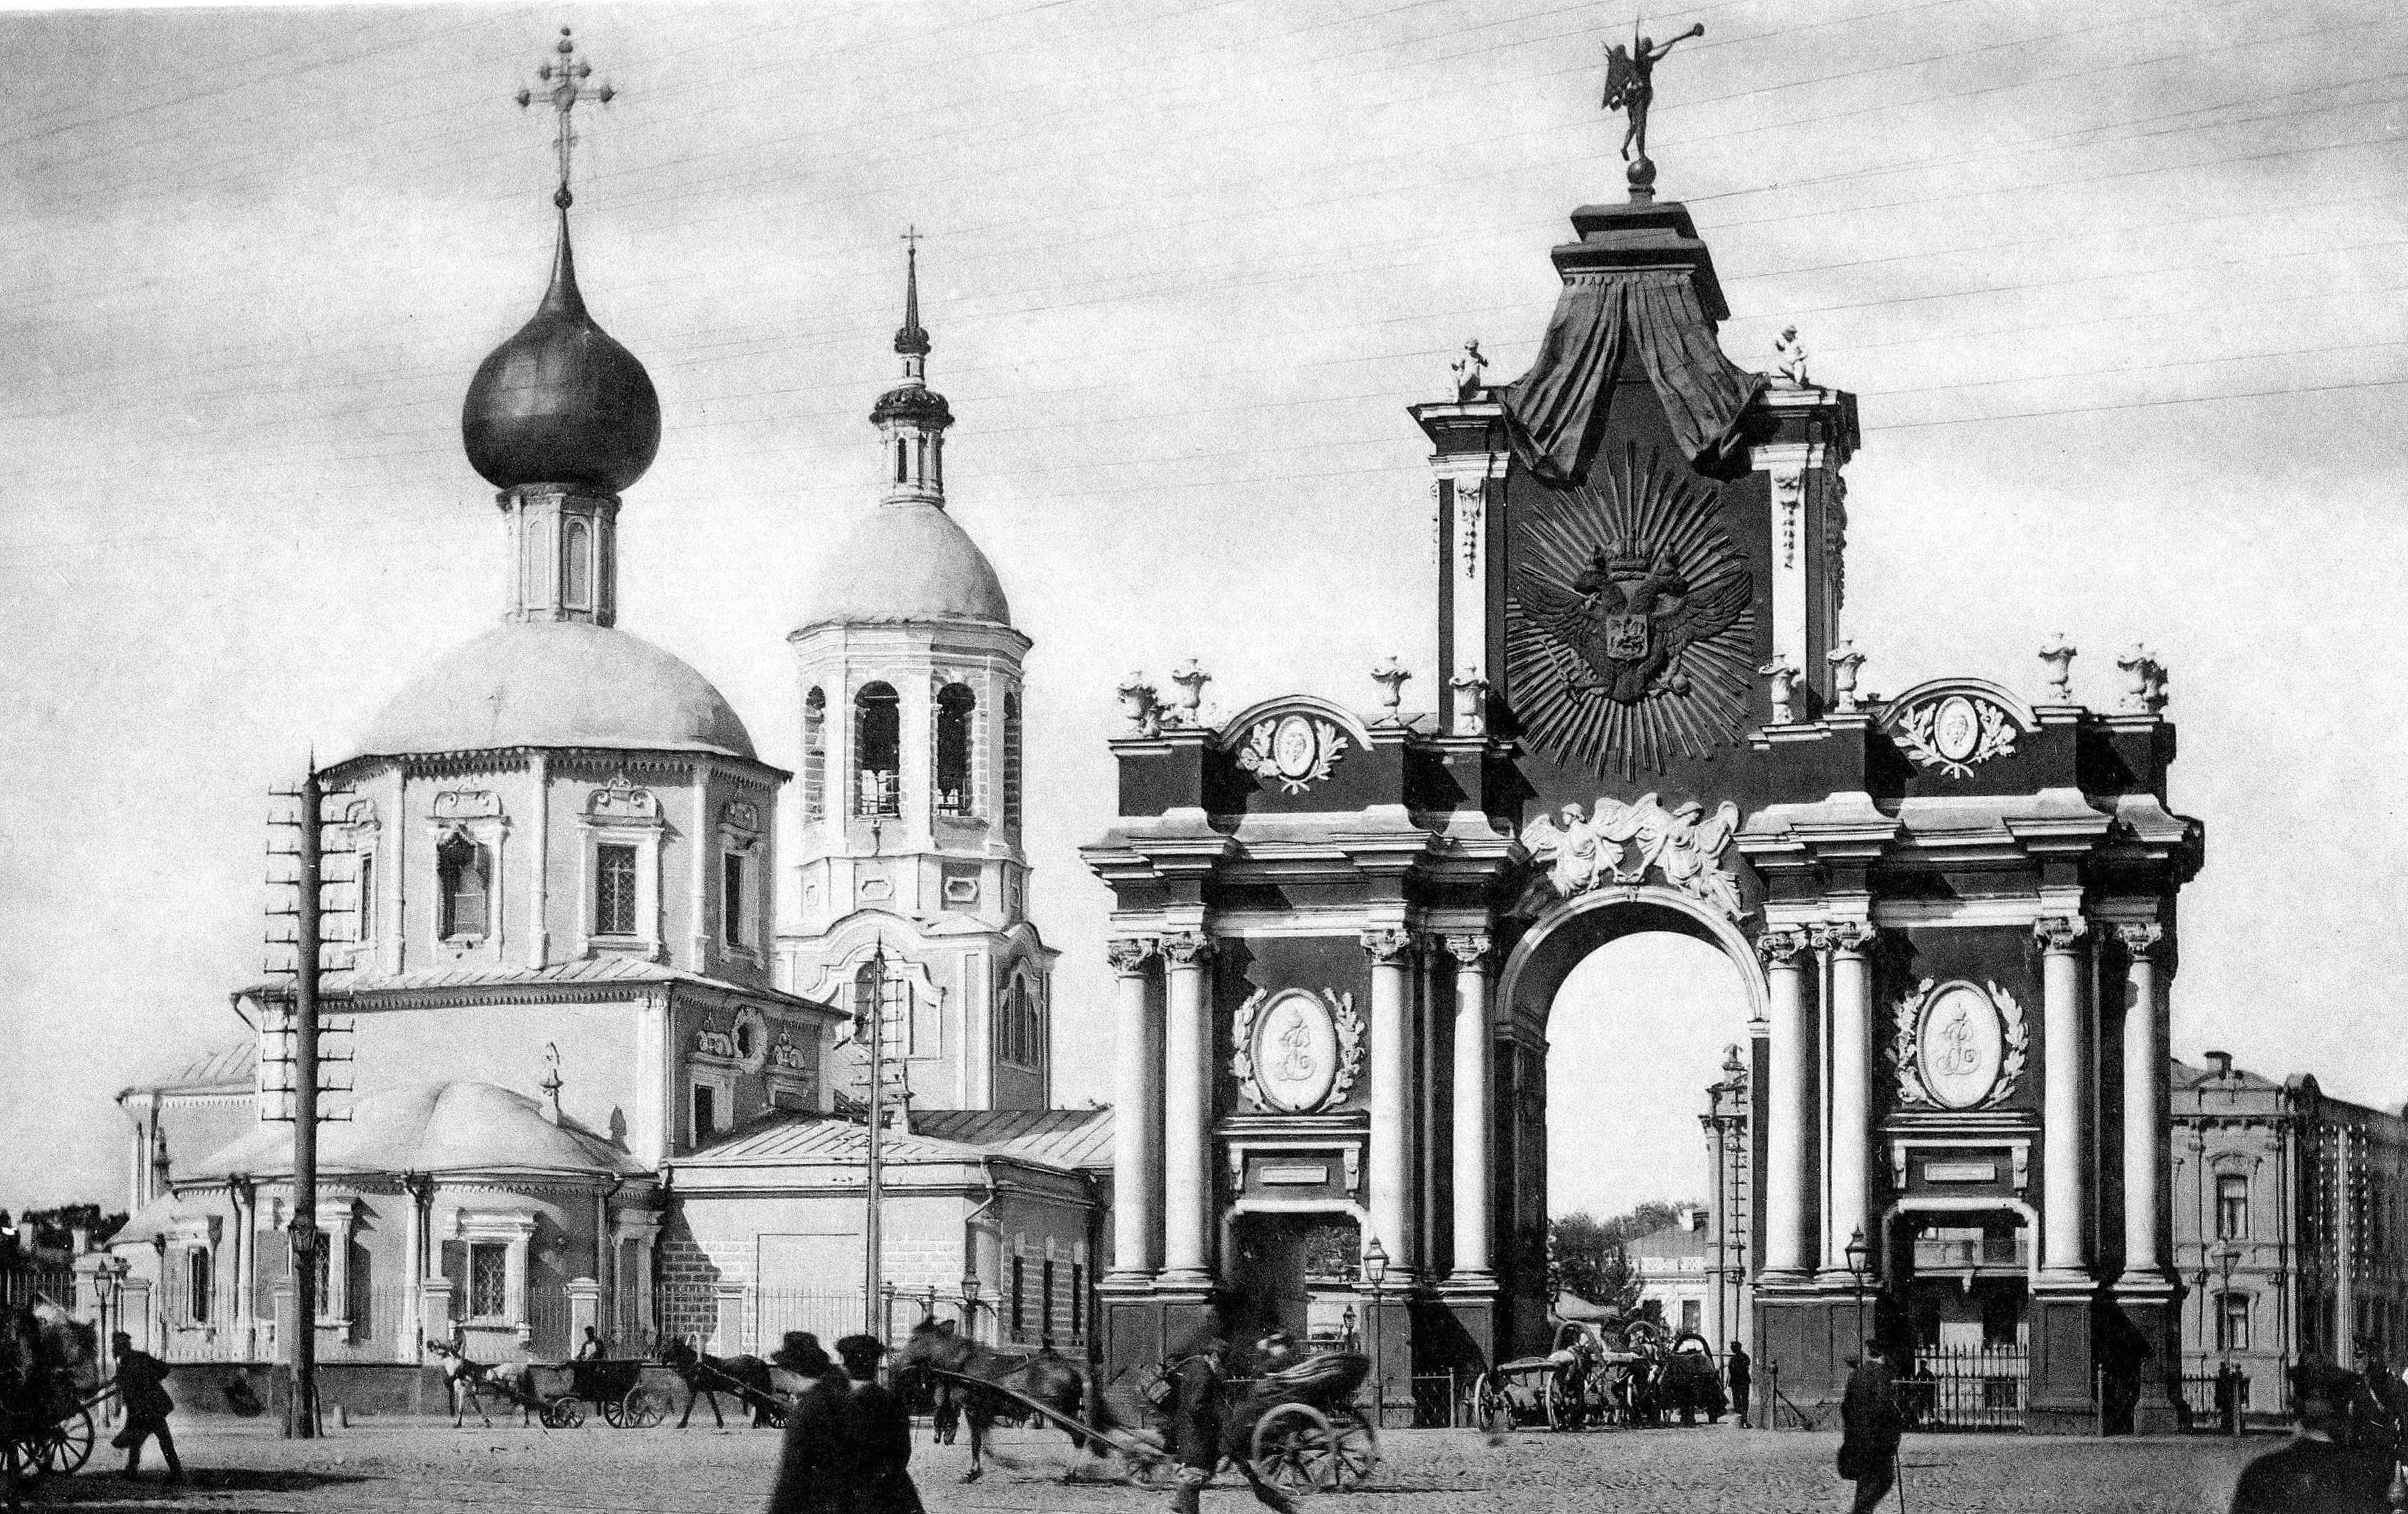
\includegraphics[width=.52\paperwidth]{inc/Title.jpg}
\end{figure}

\vfill

2012

\end{center}

\newpage

\thispagestyle{empty} 


\newgeometry{top=5cm,left=4cm,right=35mm}


\textit{Как и все предыдущие мои книжки, эту также набрал, оформил и отпечатал сын Миникс В. М.}



\newpage
\restoregeometry


\chapter{Предисловие}

\noindent
Совет ветеранов микрорайона, куда входит дом 2/6 по Хоромному тупику~-- Дом у Красных ворот, под руководством Т. В. Меньшиковой, которая продолжает дело своего отца, ведет подготовку к выпуску памятного альбома, посвященного истории и людям этого дома.

\vspace{10pt}

\begin{figure}[ht]
  \centering
  \begin{minipage}{7cm}
  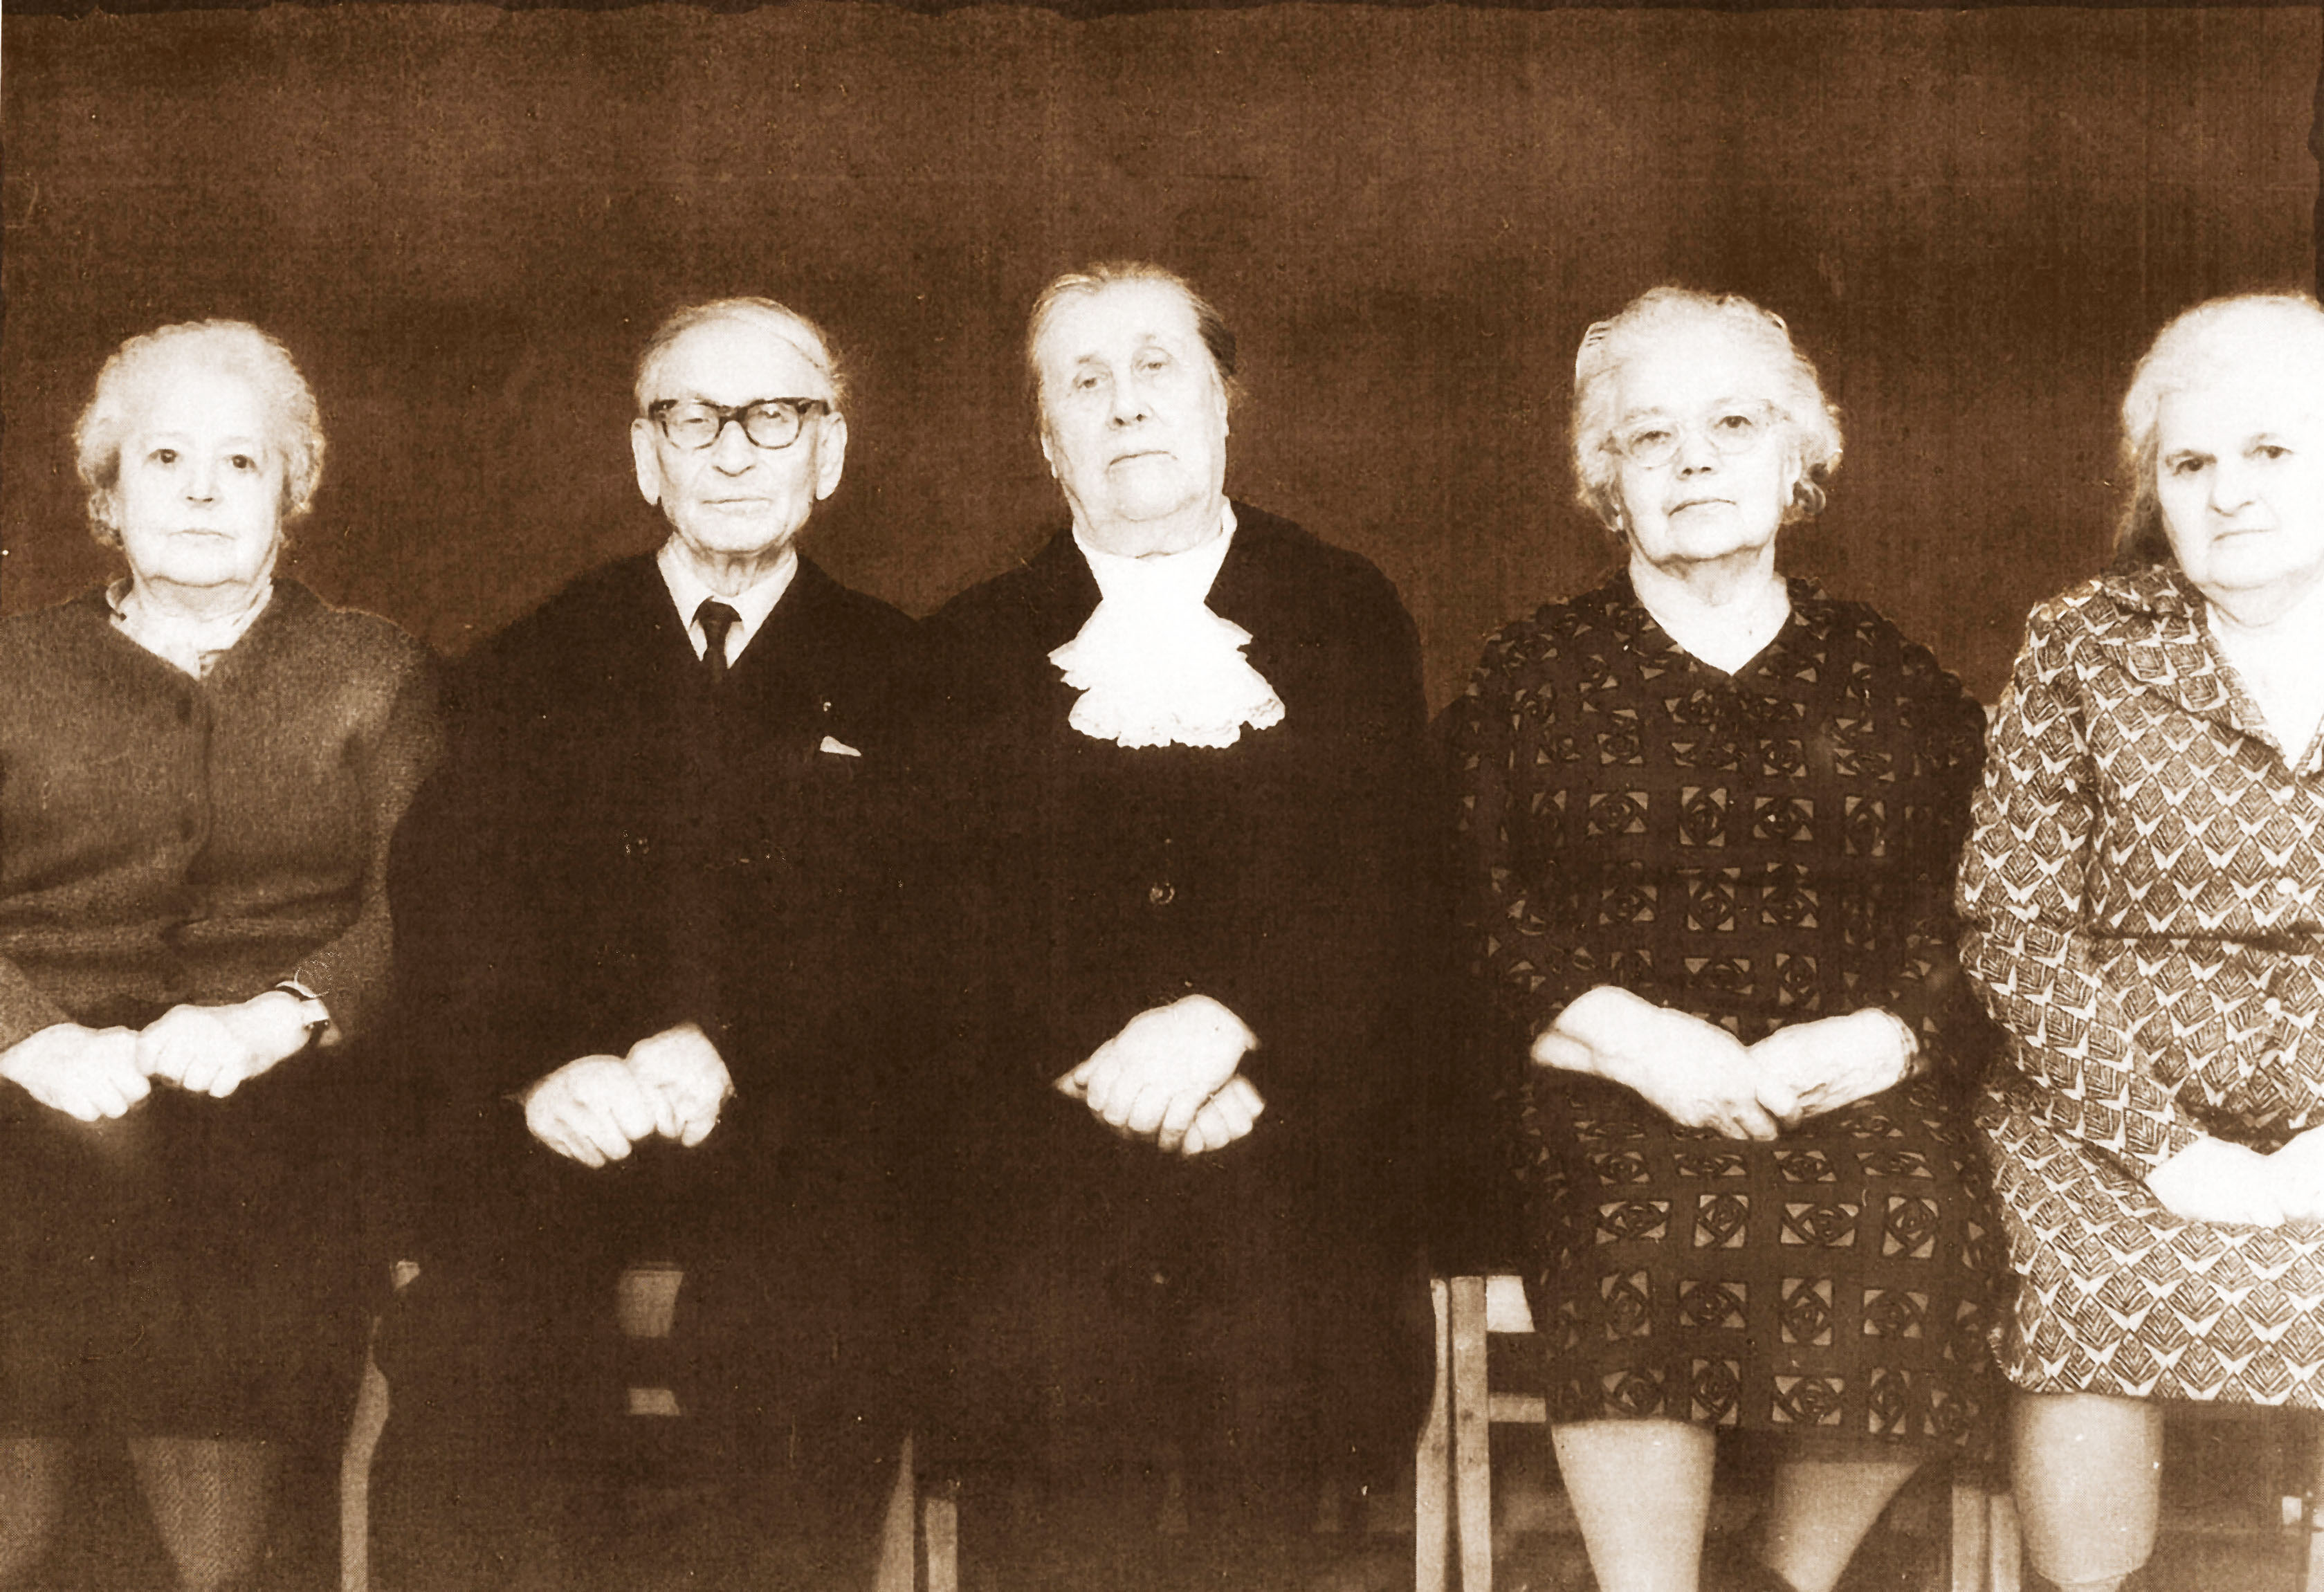
\includegraphics[width=7cm]{inc/3/1}
  \textit{\footnotesize{ Старший по Дому Меньшиков В. А. и его гвардия из <<первопоселенцев>>.}}
  \end{minipage}
\end{figure}

Предполагается, по-возможности, собрать и в систематизированном виде представить фактические данные и фотографии, в первую очередь относящиеся к <<первопоселенцам>> и семьям, въехавшим в дом в тридцатых-сороковых годах прошлого века.

Фотографии, представленные здесь, хорошо бы дополнить видом площади с <<живыми>> Красными воротами, а может быть и другими.

Вводный раздел, кроме статьи авторов-составителей Т. В. Меньшиковой и К. Д. Варзар, мне кажется, хорошо бы дополнить отрывками об истории Дома из воспоминаний ветеранов (см. Приложения).

Если удастся добраться до архивных документов~-- старых домовых книг, будет дан полный поквартирный список <<первопоселенцев>> и <<второпоселенцев>> (30-е, 40-е годы).

Совет ветеранов провел большую работу по формированию, проверке и систематизации списков репрессированных жильцов Дома, в первую очередь в 1937~-- 1939 гг., и реабилитированных (часто~-- посмертно) в 1956 г. <<за отсутствием состава преступления>>. Соответствующие списки будут опубликованы в Альбоме.

Этот Совет долгие годы занят благородным делом~-- помогает ветеранам Великой Отечественной войны, рассказывает о них, отмечает с ними торжественные события и памятные даты, что, конечно же, тоже будет отражено в Альбоме. Особая страница будет посвящена погибшим на этой войне. Не будут забыты и герои тыла.

Хорошо было бы по самостоятельной странице посвятить жильцам~-- семьям каждой из 97 квартир Дома. Но, к сожалению, через столько десятилетий раздобыть исчерпывающие данные, а особенно фото, невозможно.
Поэтому придется опубликовать только то, что удастся собрать. 

Ниже для примера в алфавитном порядке приведены данные\footnote{В Альбоме такие композиции будут размером 20 на 30 см.} о шести семьях: Варзаров, Кузнецовых, Меньшиковых, Миниксов, Моргуновых и Плоткиных.


\newgeometry{left=0mm, right=0mm, top=0mm, bottom=0mm}

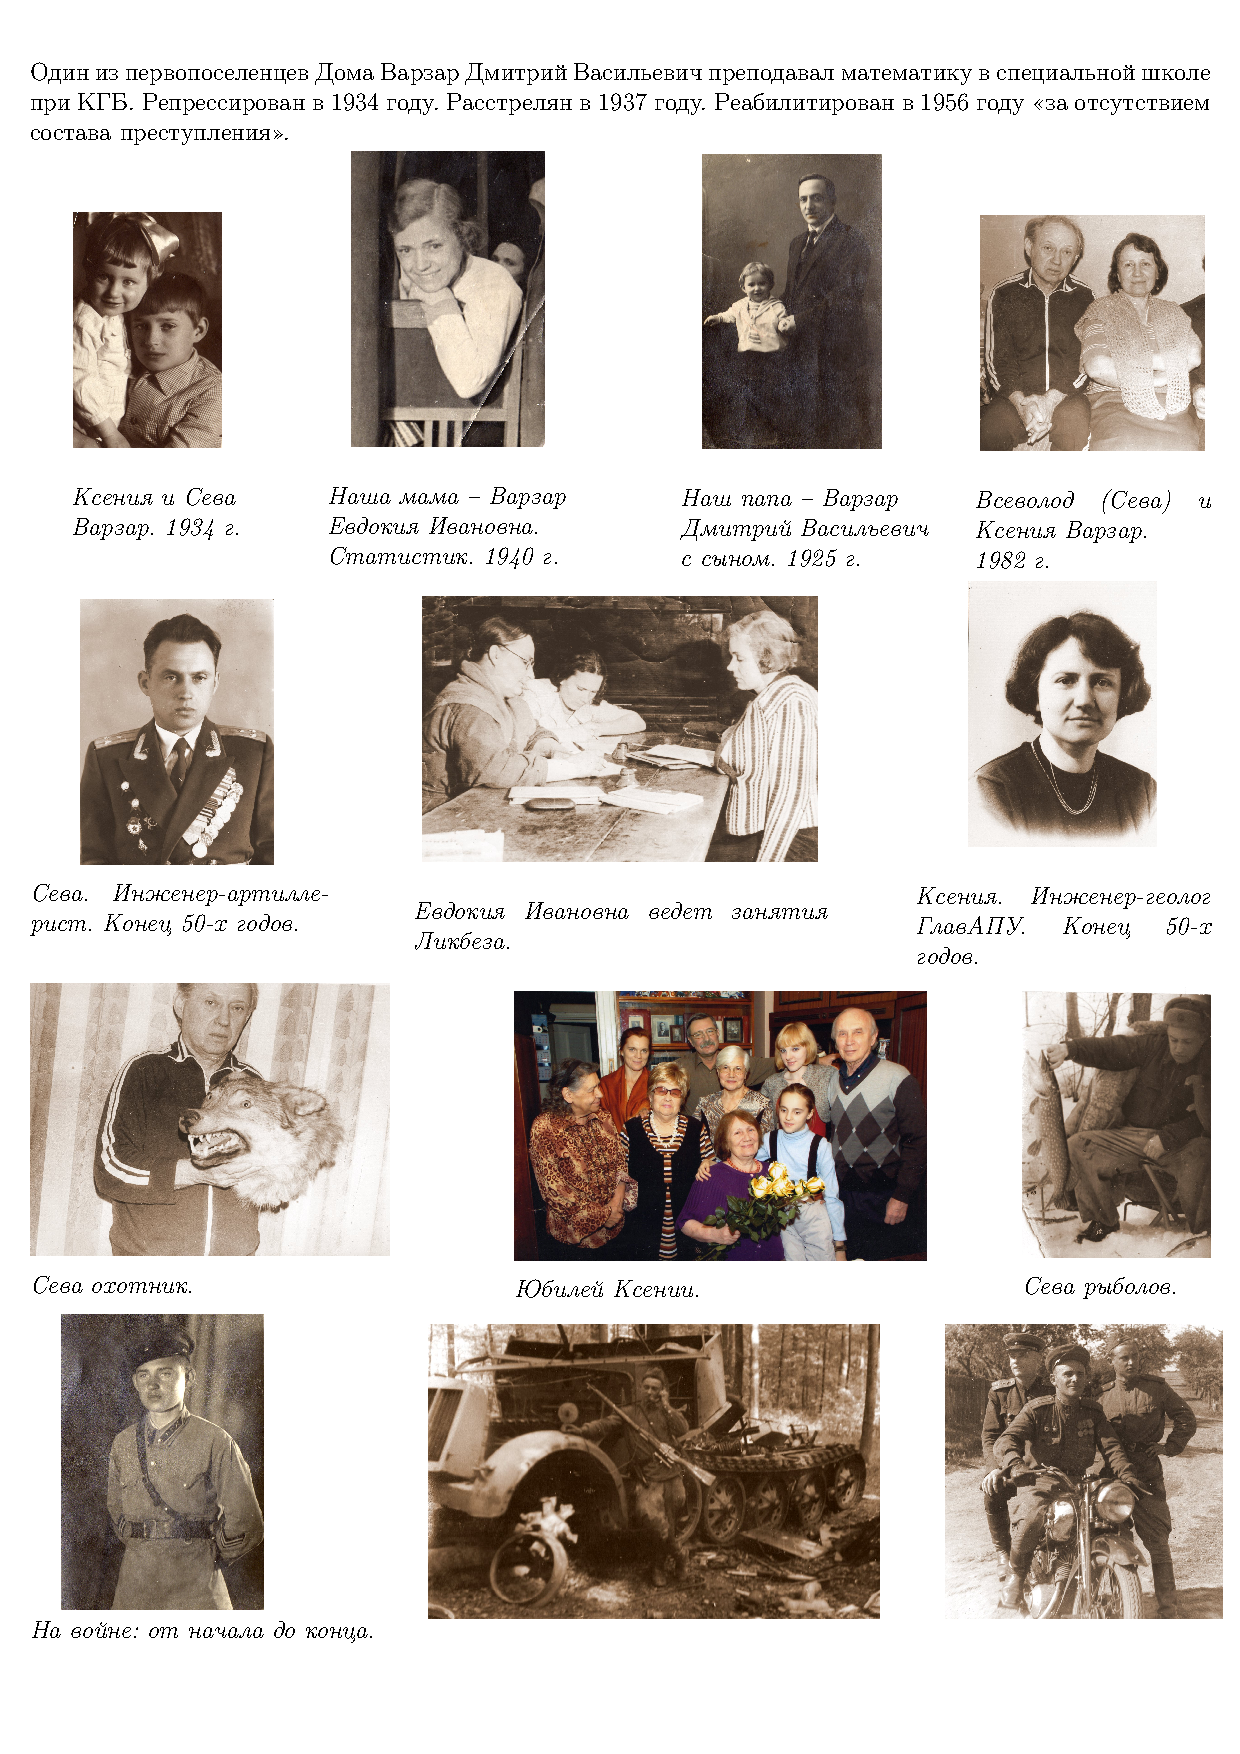
\includepdf[pages=-]{inc/varzar.pdf}

\noindent
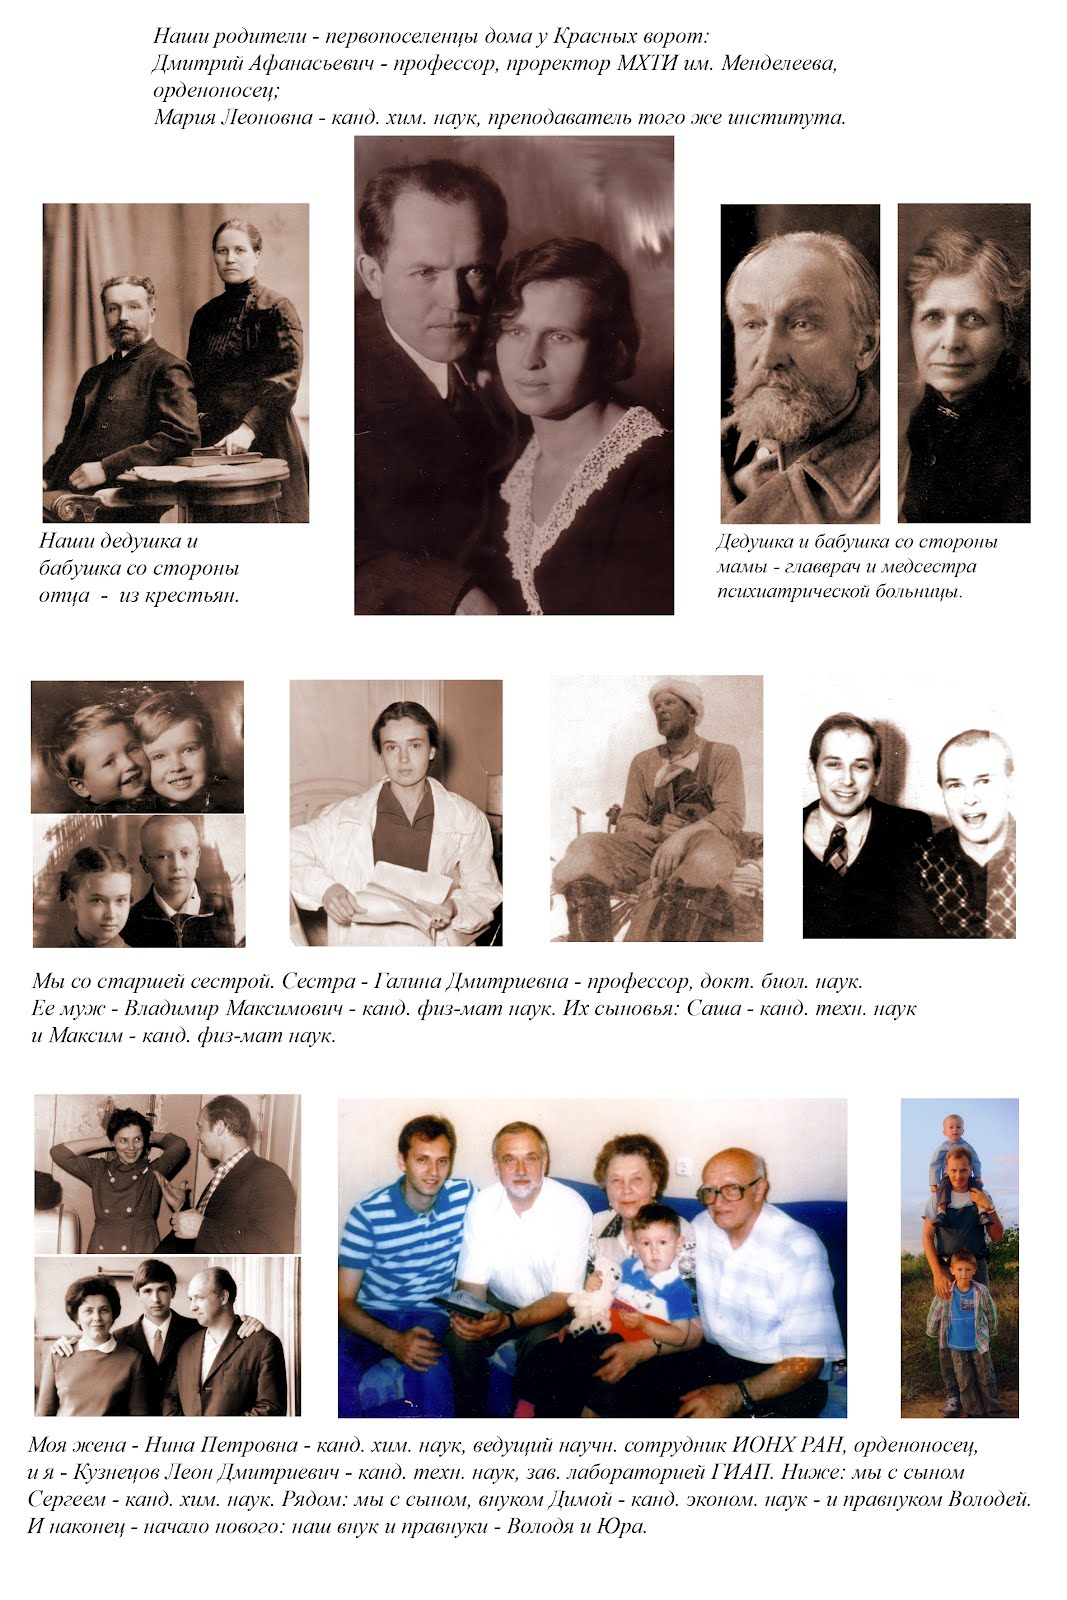
\includegraphics[height=\paperheight]{inc/kuznecovy}


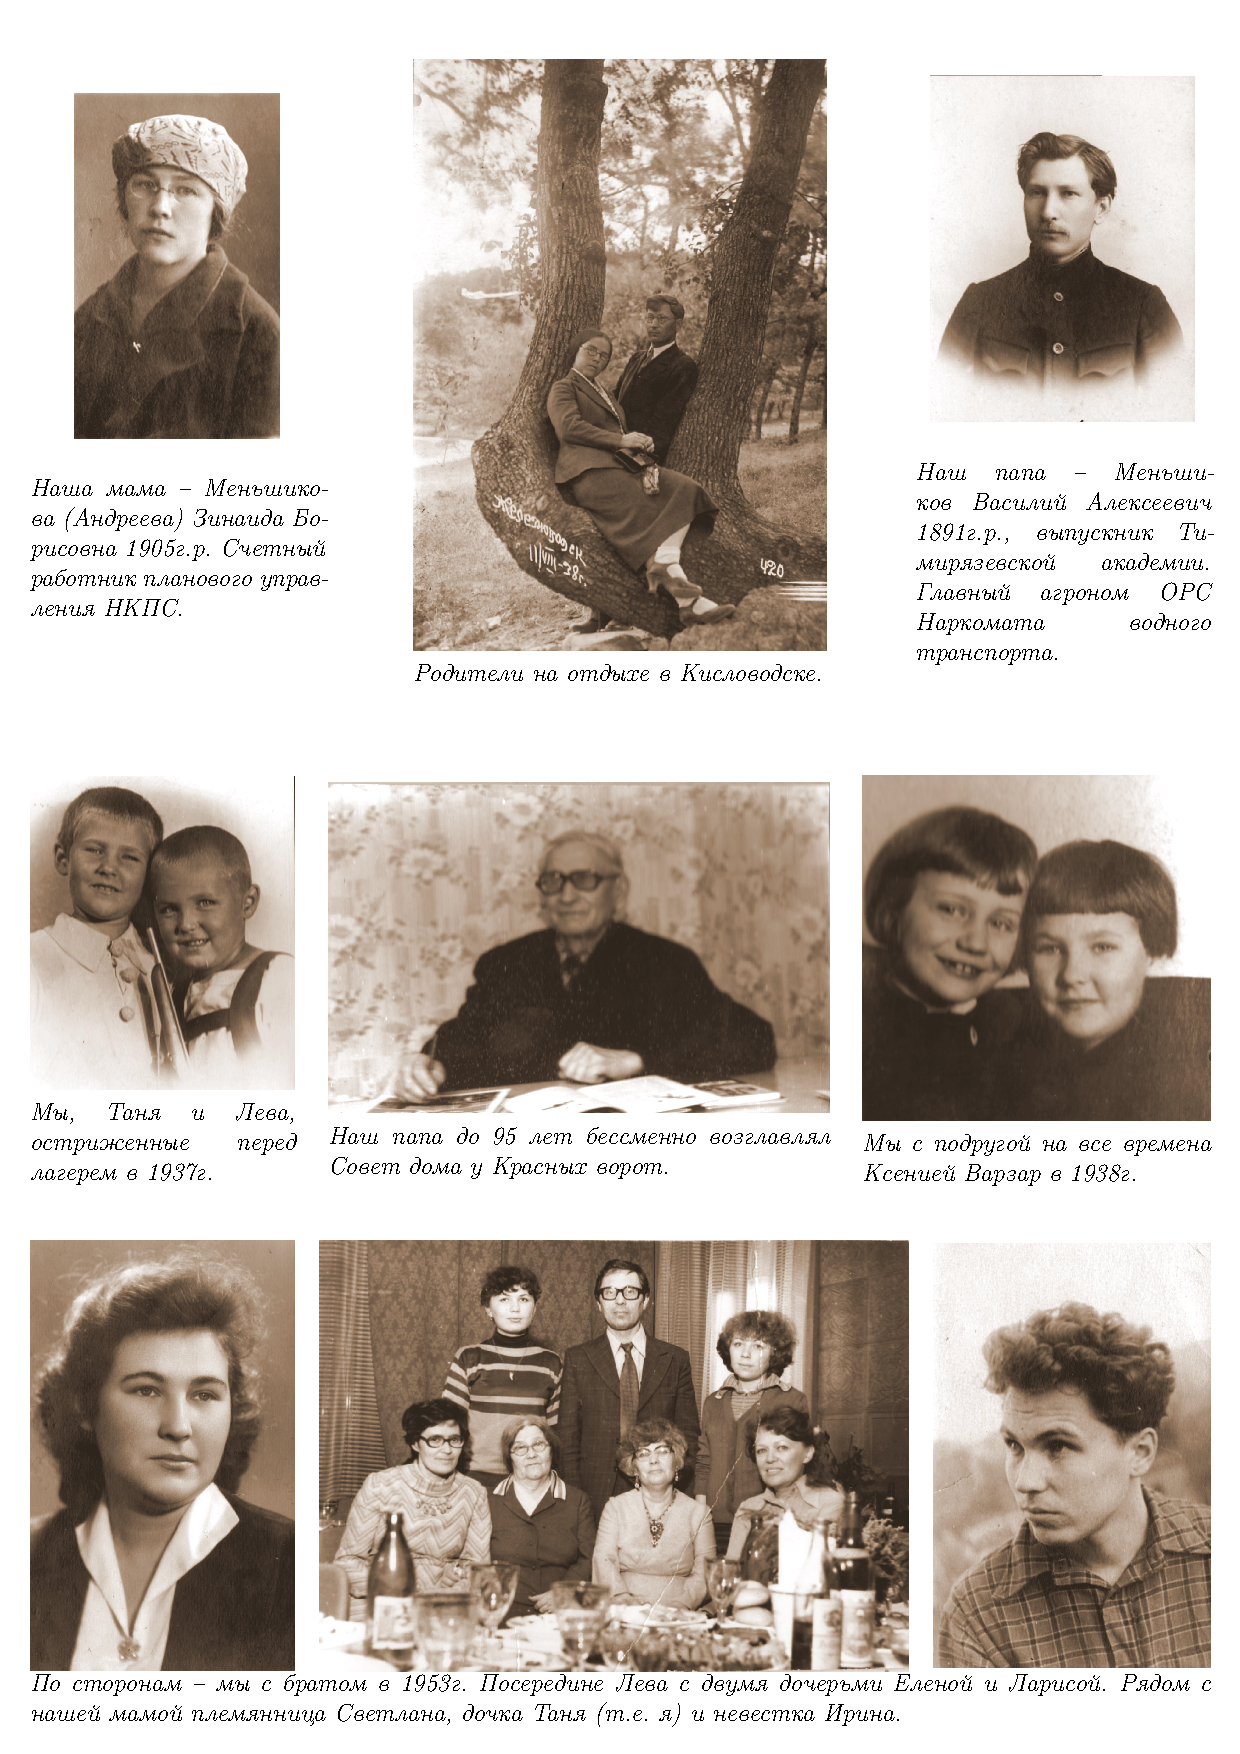
\includepdf[pages=-]{inc/menshekovy.pdf}


\begin{center}

\noindent
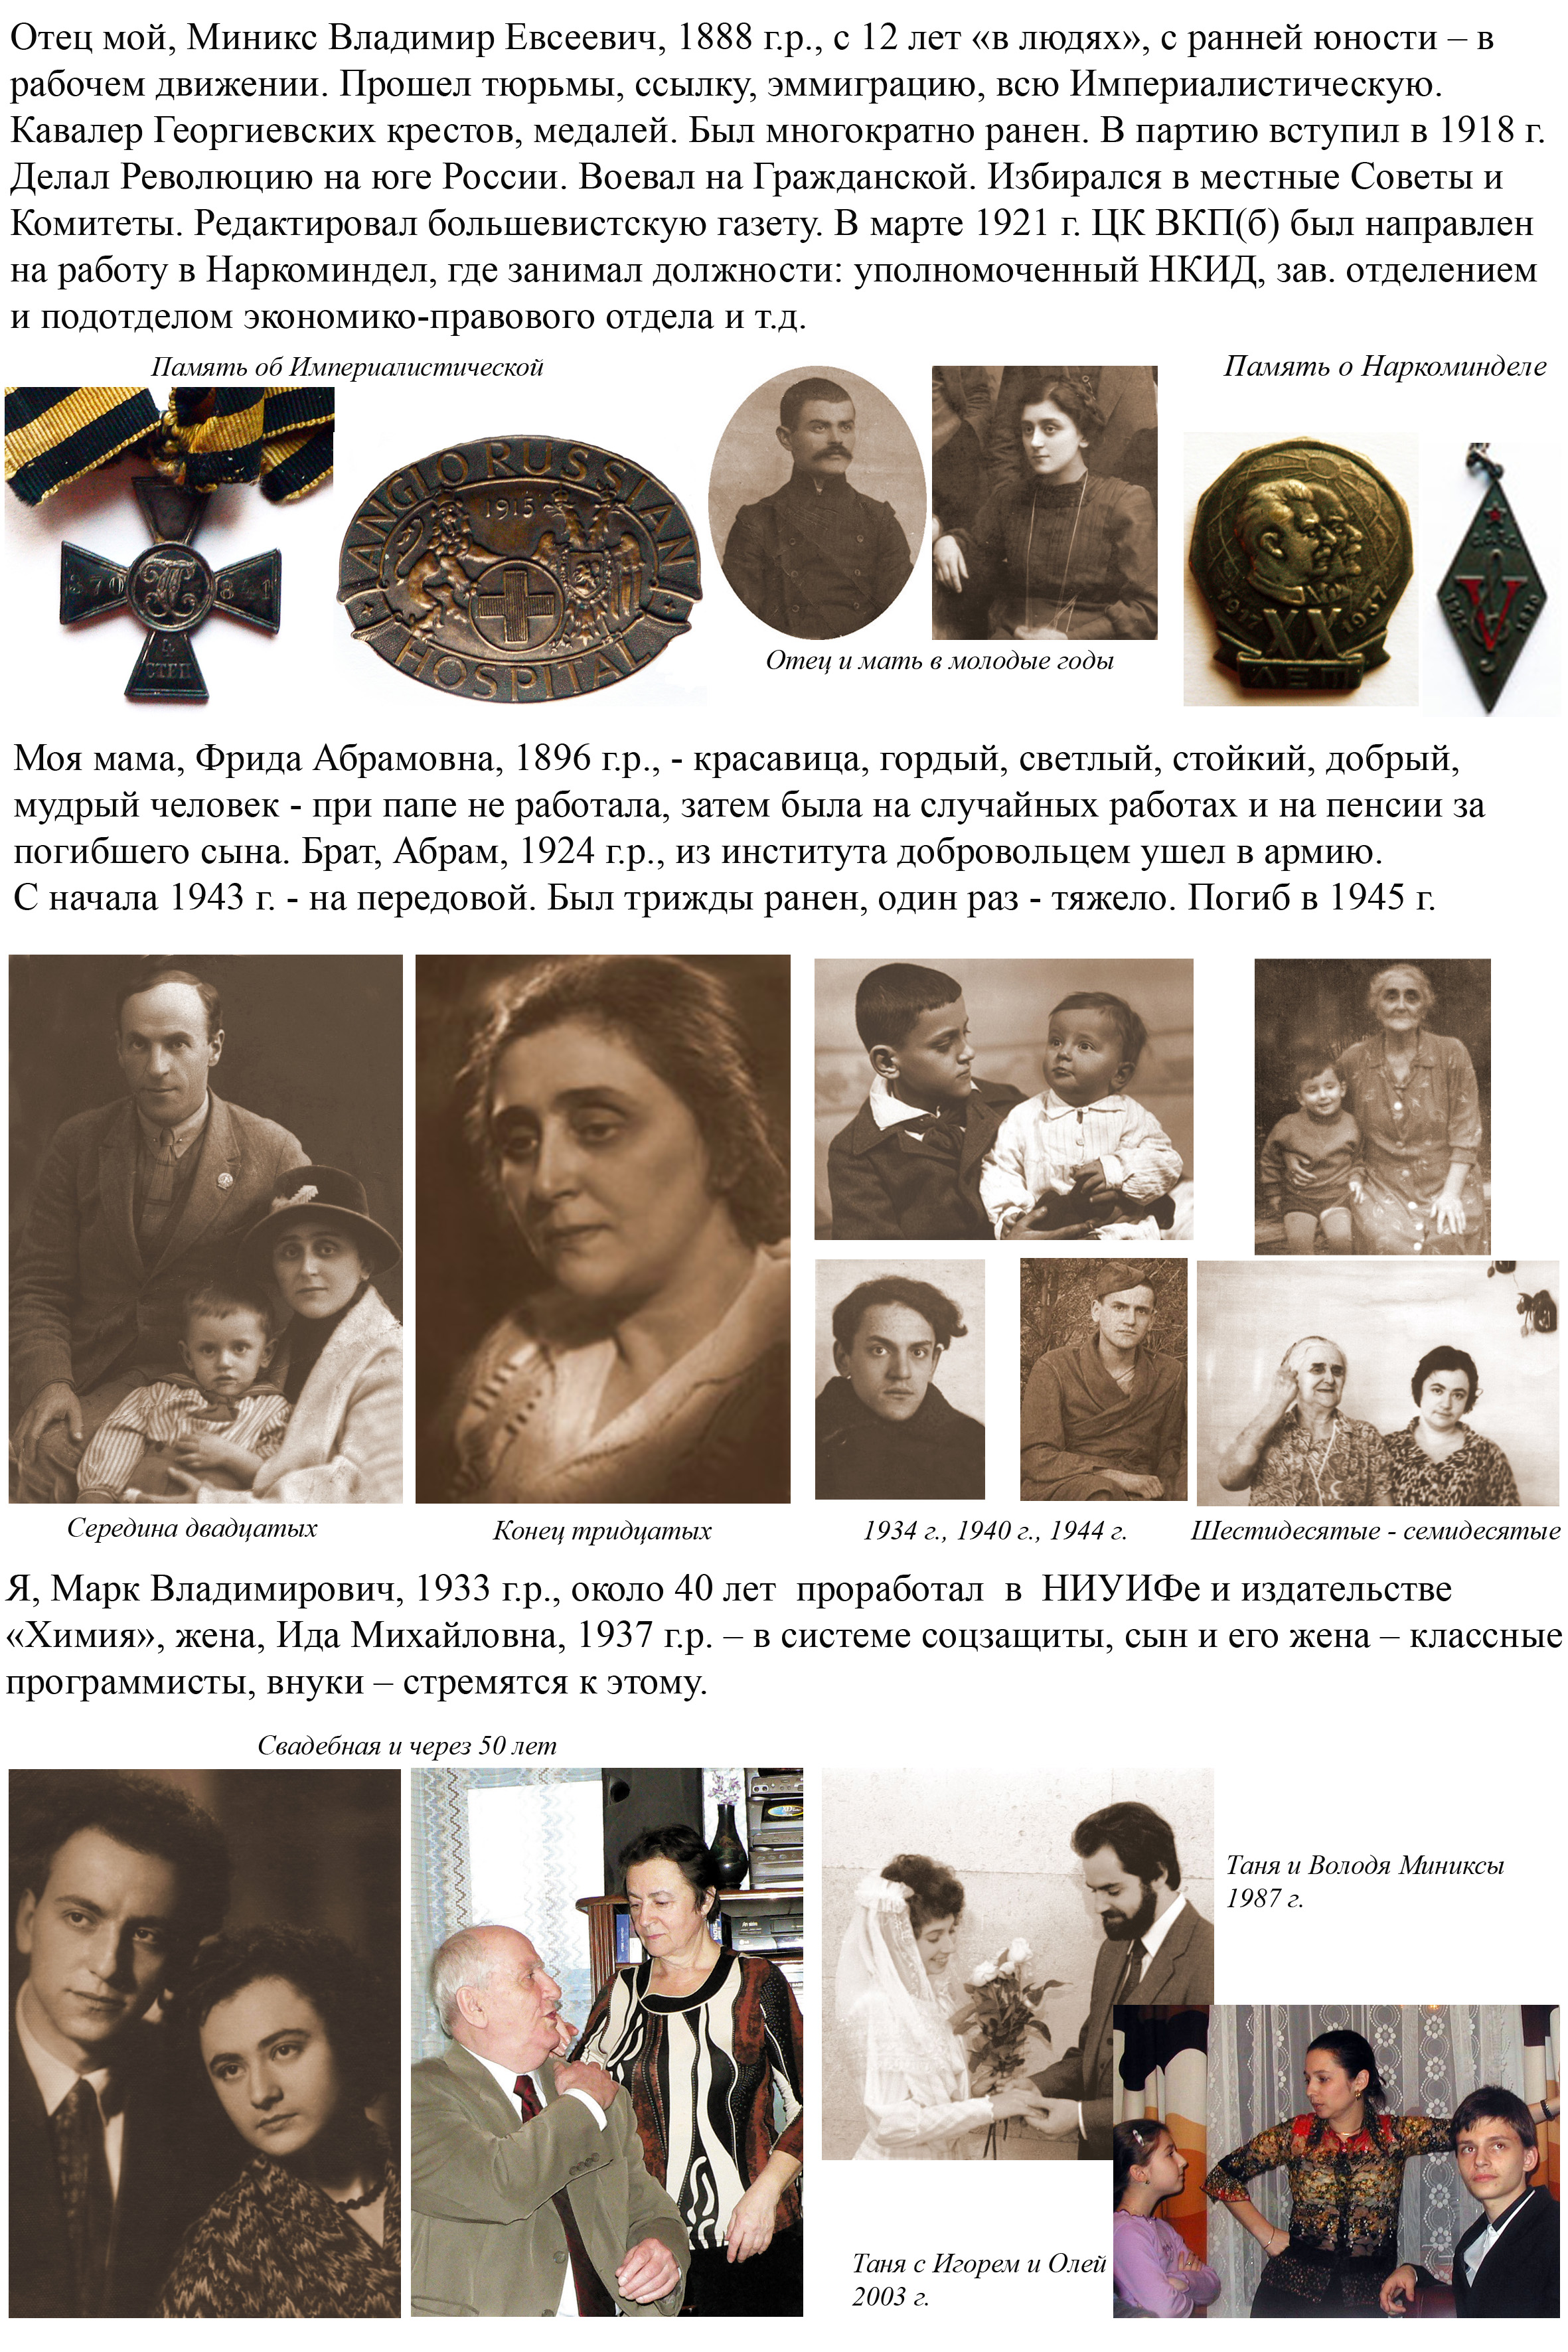
\includegraphics[height=\paperheight]{inc/minixy}

\noindent
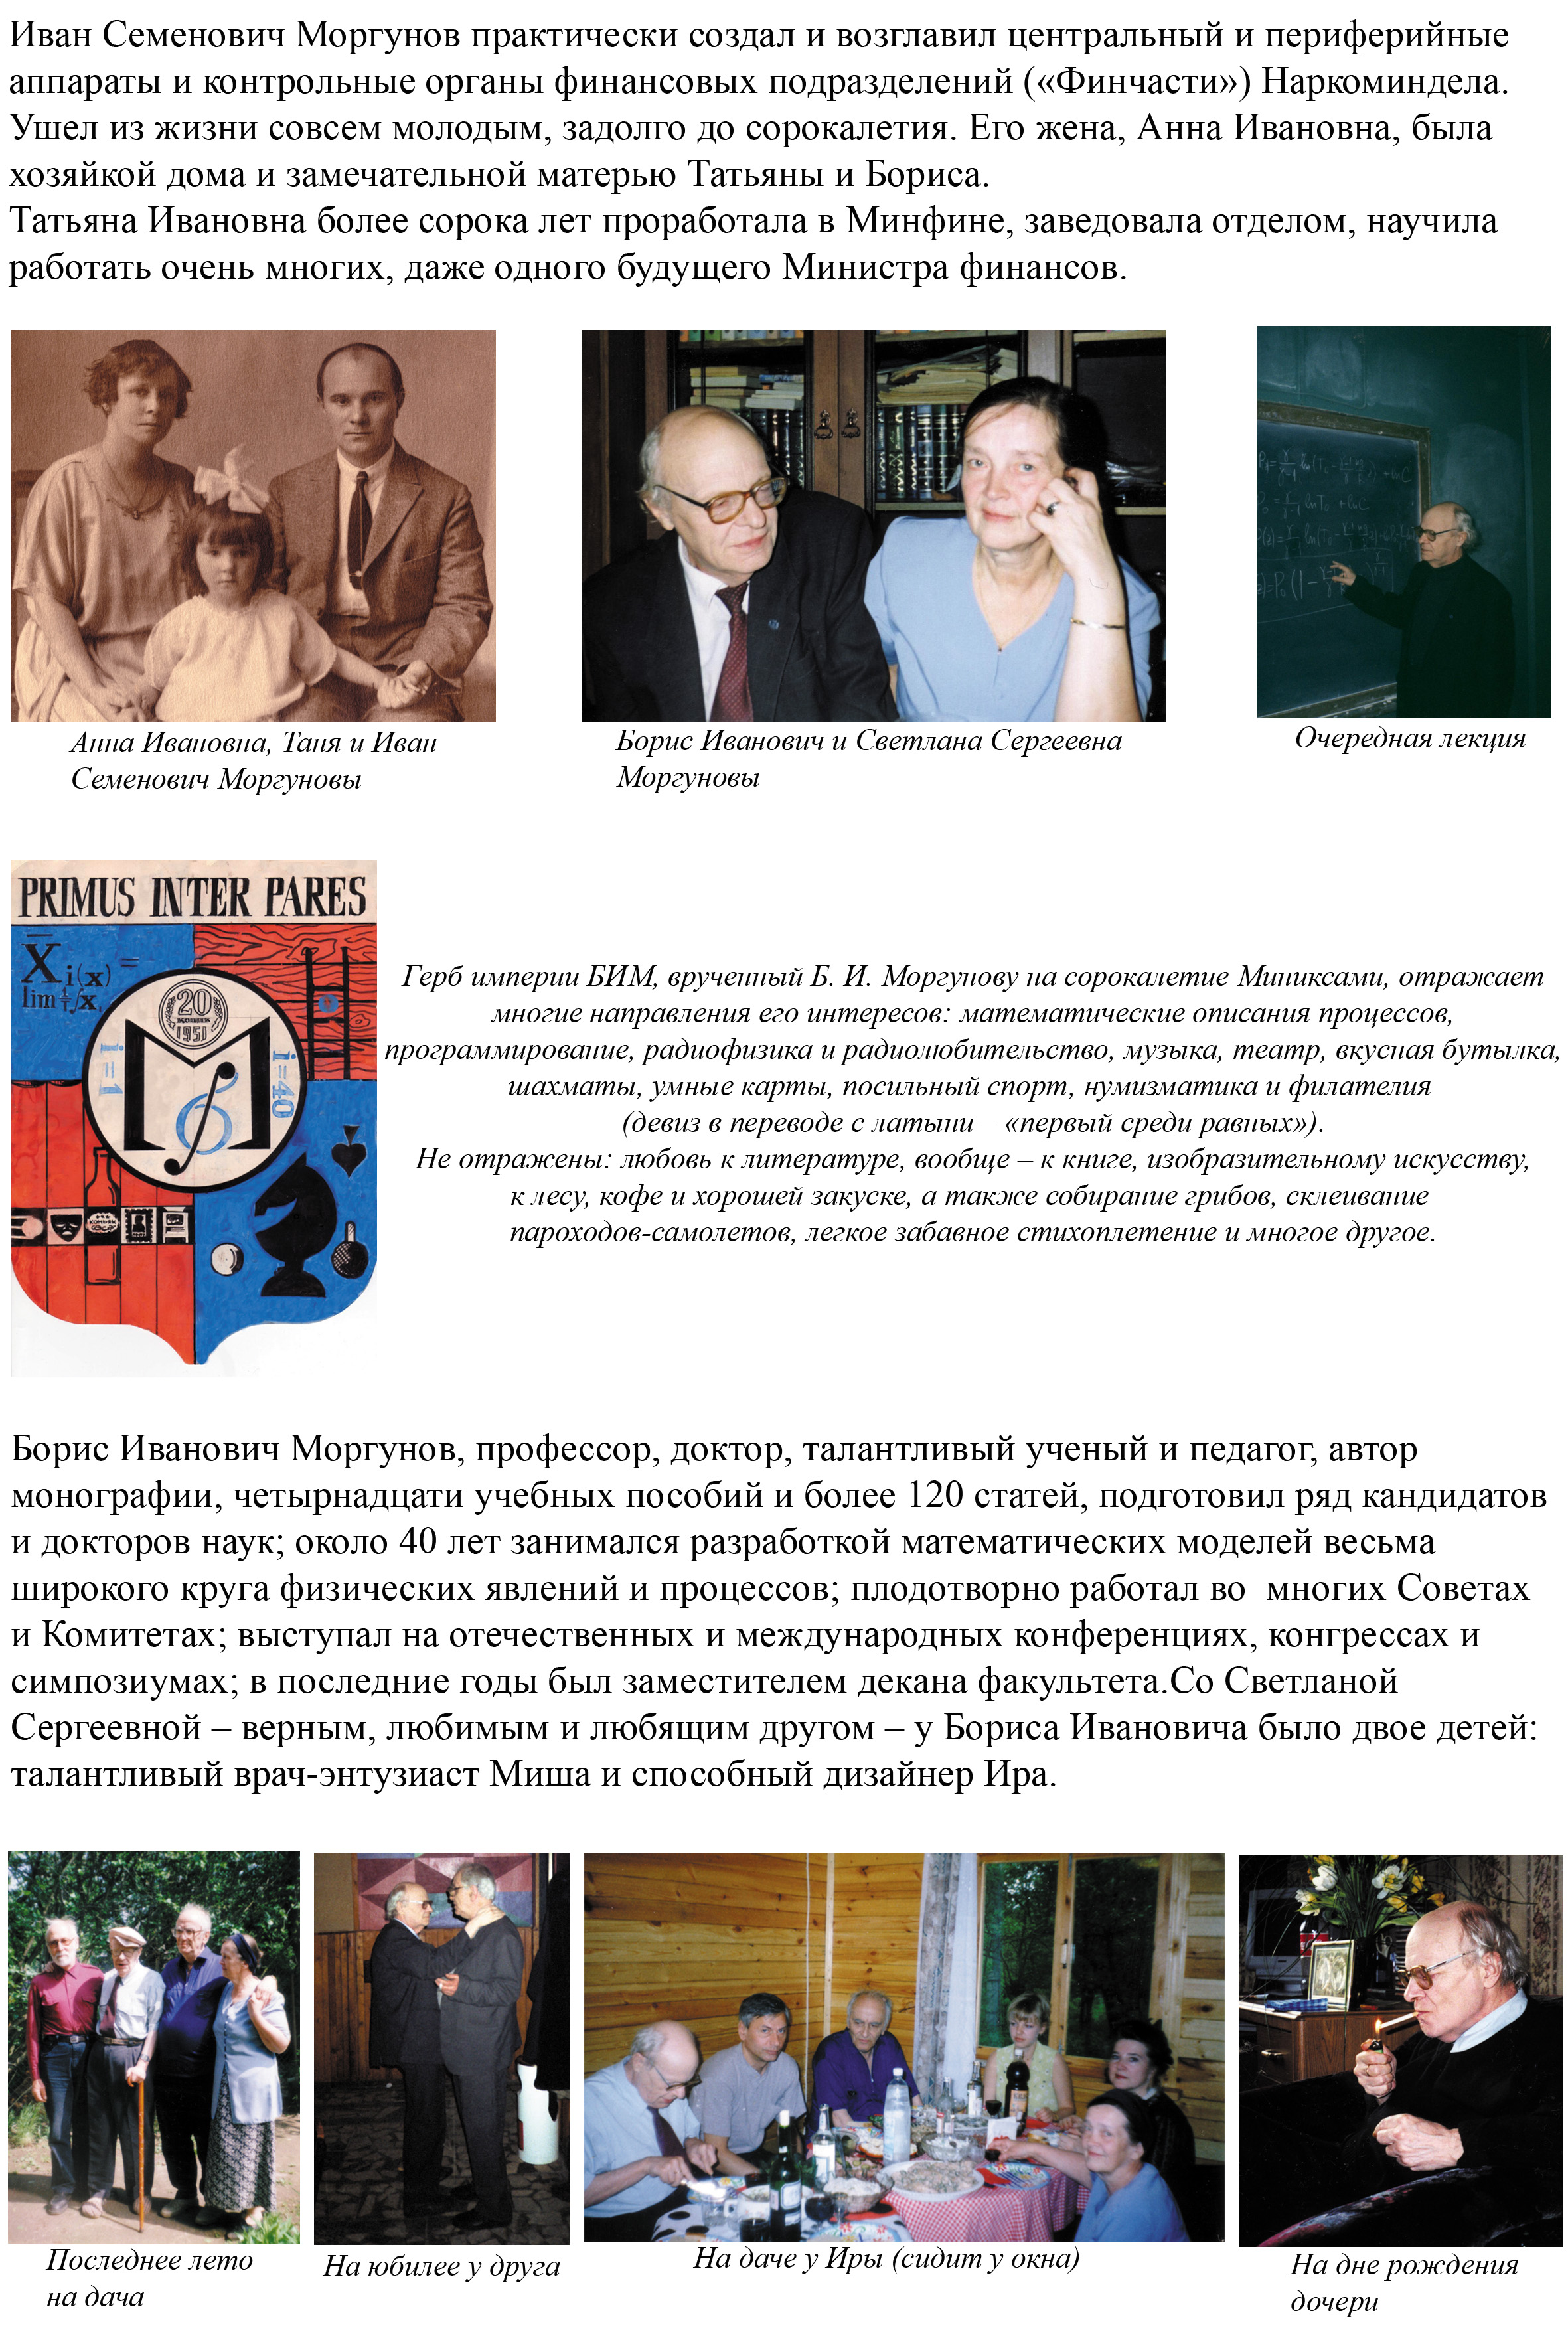
\includegraphics[height=\paperheight]{inc/morgunovy}

\noindent
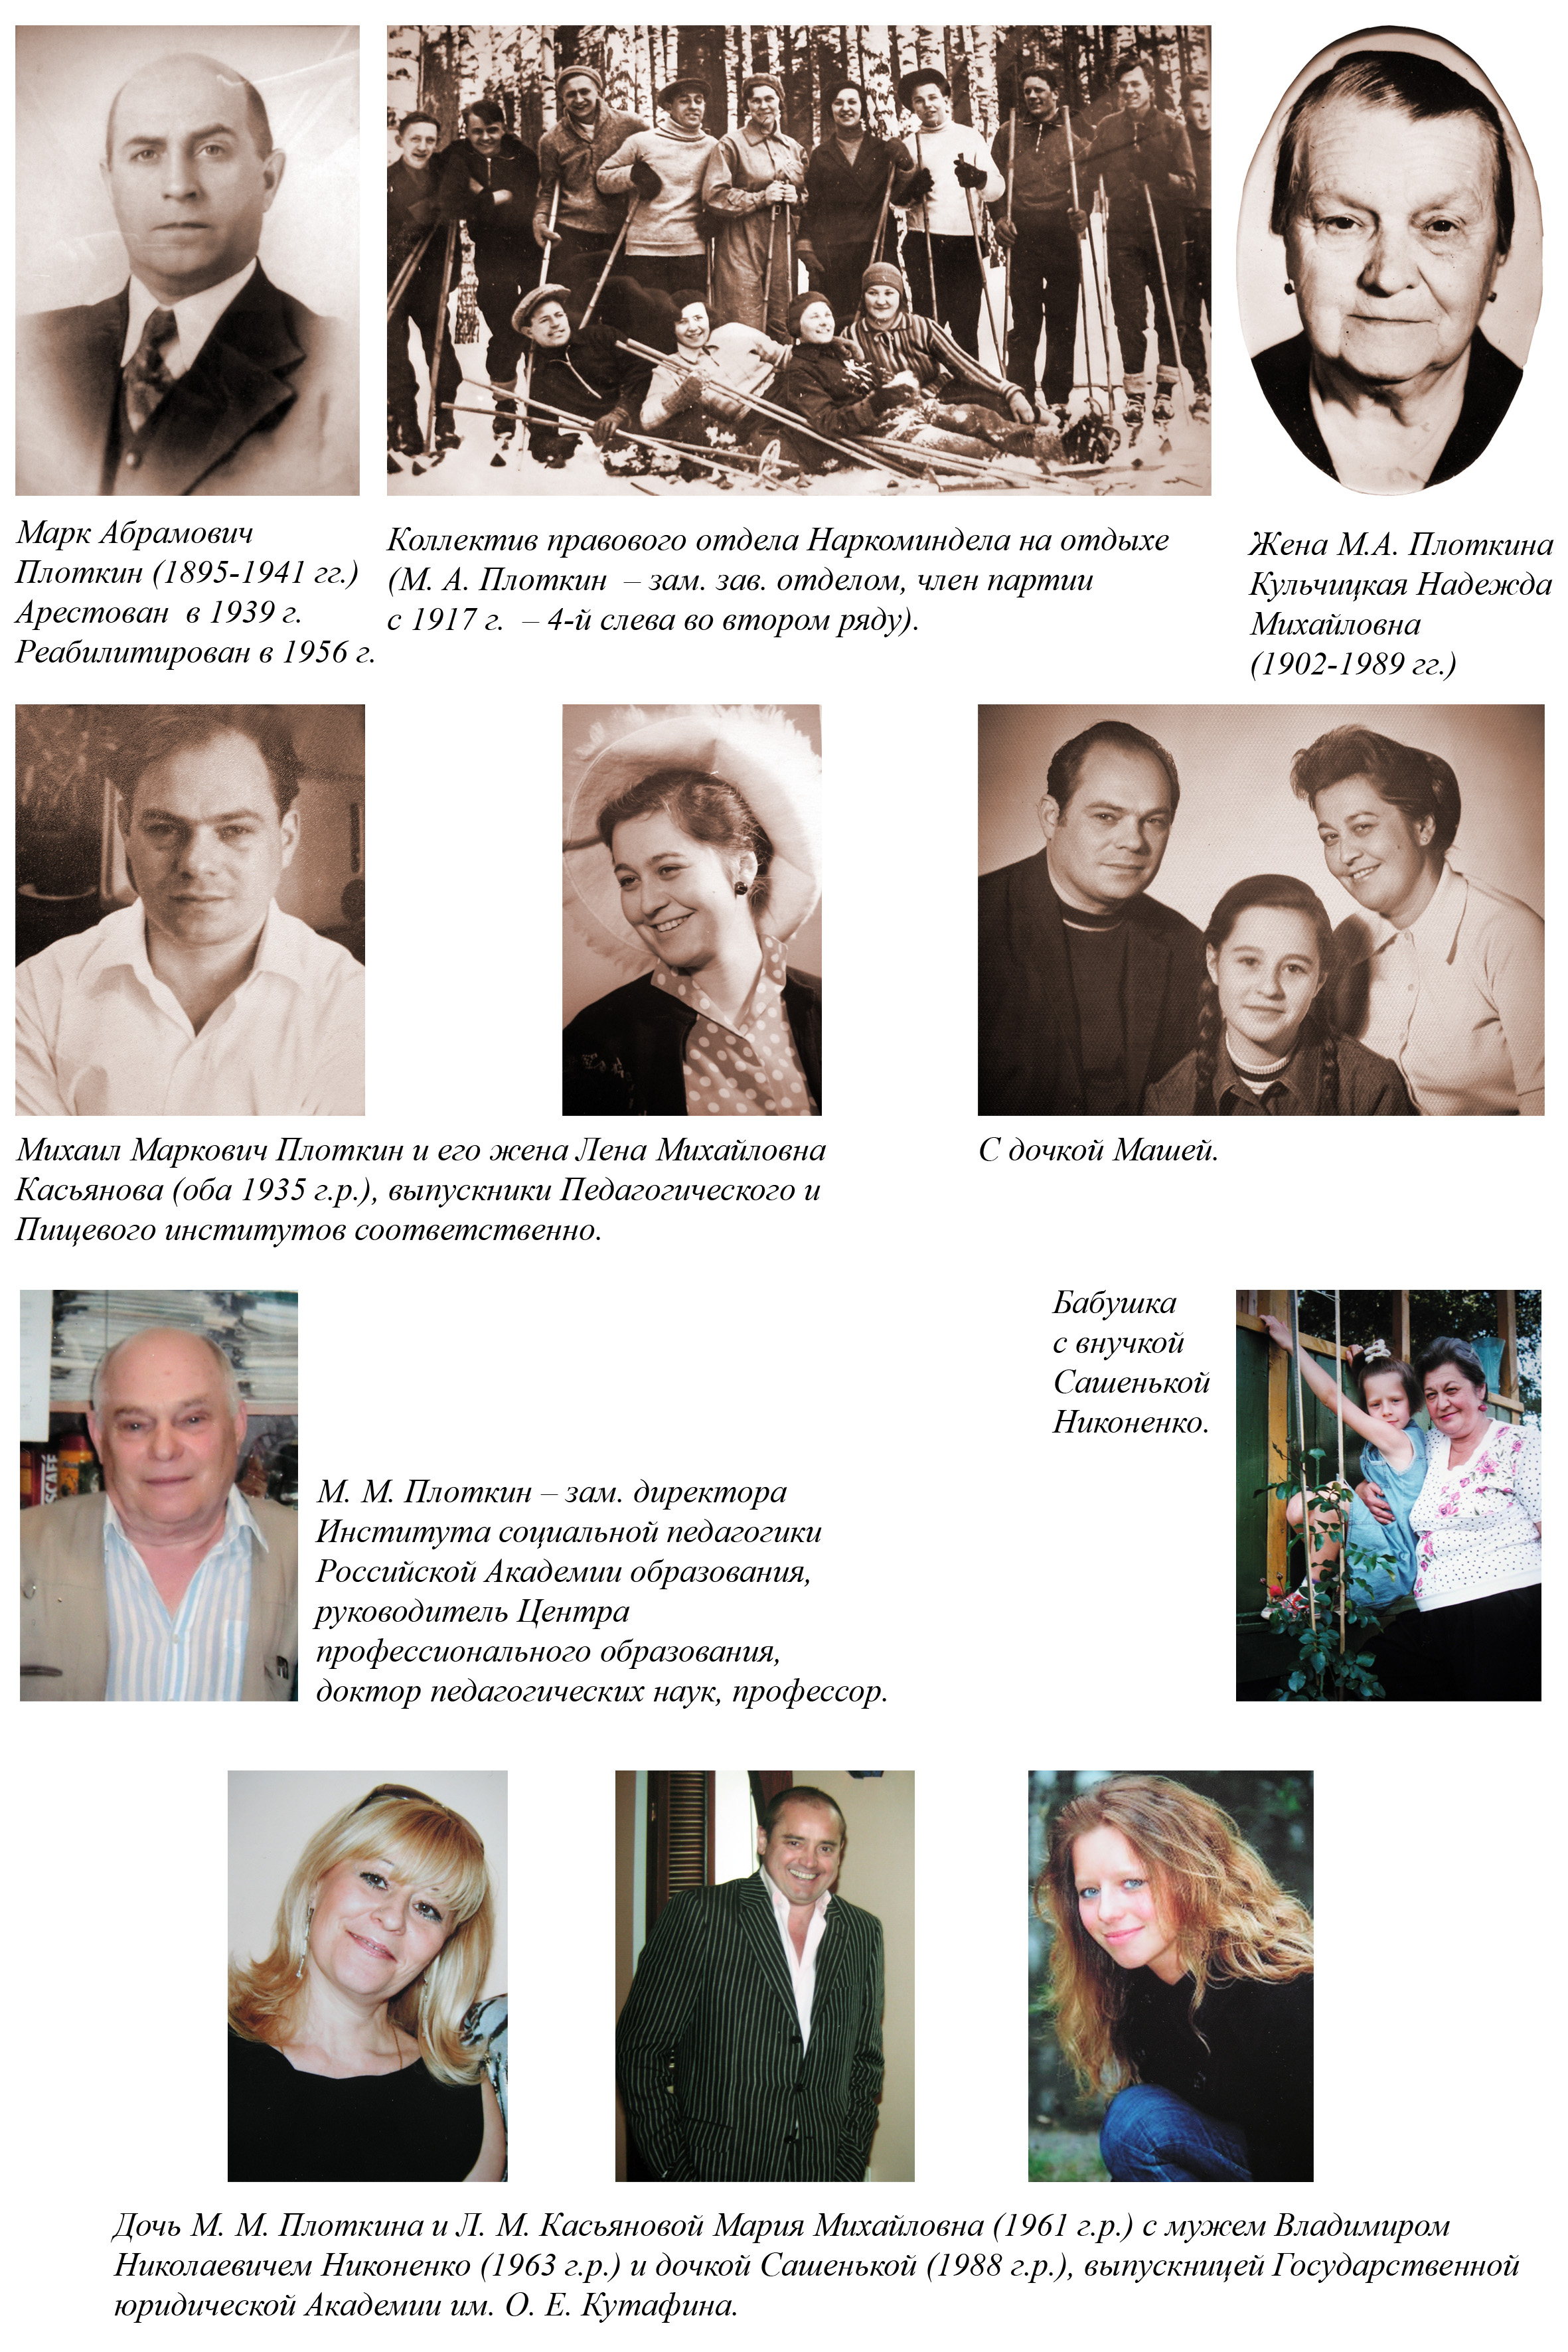
\includegraphics[height=\paperheight]{inc/plotkiny}

\end{center}

\restoregeometry



\chapter{Дворовые компании}

Многие данные и фоотографии предоставлены мне Т. В. Меньшиковой. Ей же благодарен за добрые советы.

Мне поручили написать о дворовых компанях, что я и постараюсь сделать с учетом <<собирательных>> свойств нашего Дома за период с тридцатых до шестидесятых годов. Аналог этого книжного варианта, естественно, будет в Альбоме.

Нельзя не сказать, что среди первопоселенцев нашего дома было очень много замечательных людей, начиная с Народного Комиссара иностранных дел М. М. Литвинова, его заместителей, руководителей подразделений, Чрезвычайных и полномочных посло того времени.

Сейчас, через 80 с лишним лет после заселения нашего дома, трудно сказать насколько были дружны между собой первопоселенцы, были ли дворовые компании у их старших детей (до 1920 года рождения), привлекались ли в эти компании ребята из других домов, что было характерно для последующих поколений, когда компании формировались из ребят окрестных дворов, как правило, в возрастном диапазоне 2-3 года с вкраплениями до 5 лет.

Собирательная особенность нашего двора наметилась еще до Войны, у ребят около 1924 года рождения, в основном выпускников школ 1941 года. К ним относятся: Бабенко И. Я., Багун Ю. (воевал), Варзар Сева (прошел всю войну), Дивильковский Юра (погиб), Клейн Наташа (воевала), Короткин Жора (погиб), Кунина Ляля (воевала), миникс Аба (погиб).

\newpage % ??
\newgeometry{left=10mm, right=10mm, top=5mm, bottom=0mm}

\begin{center}
    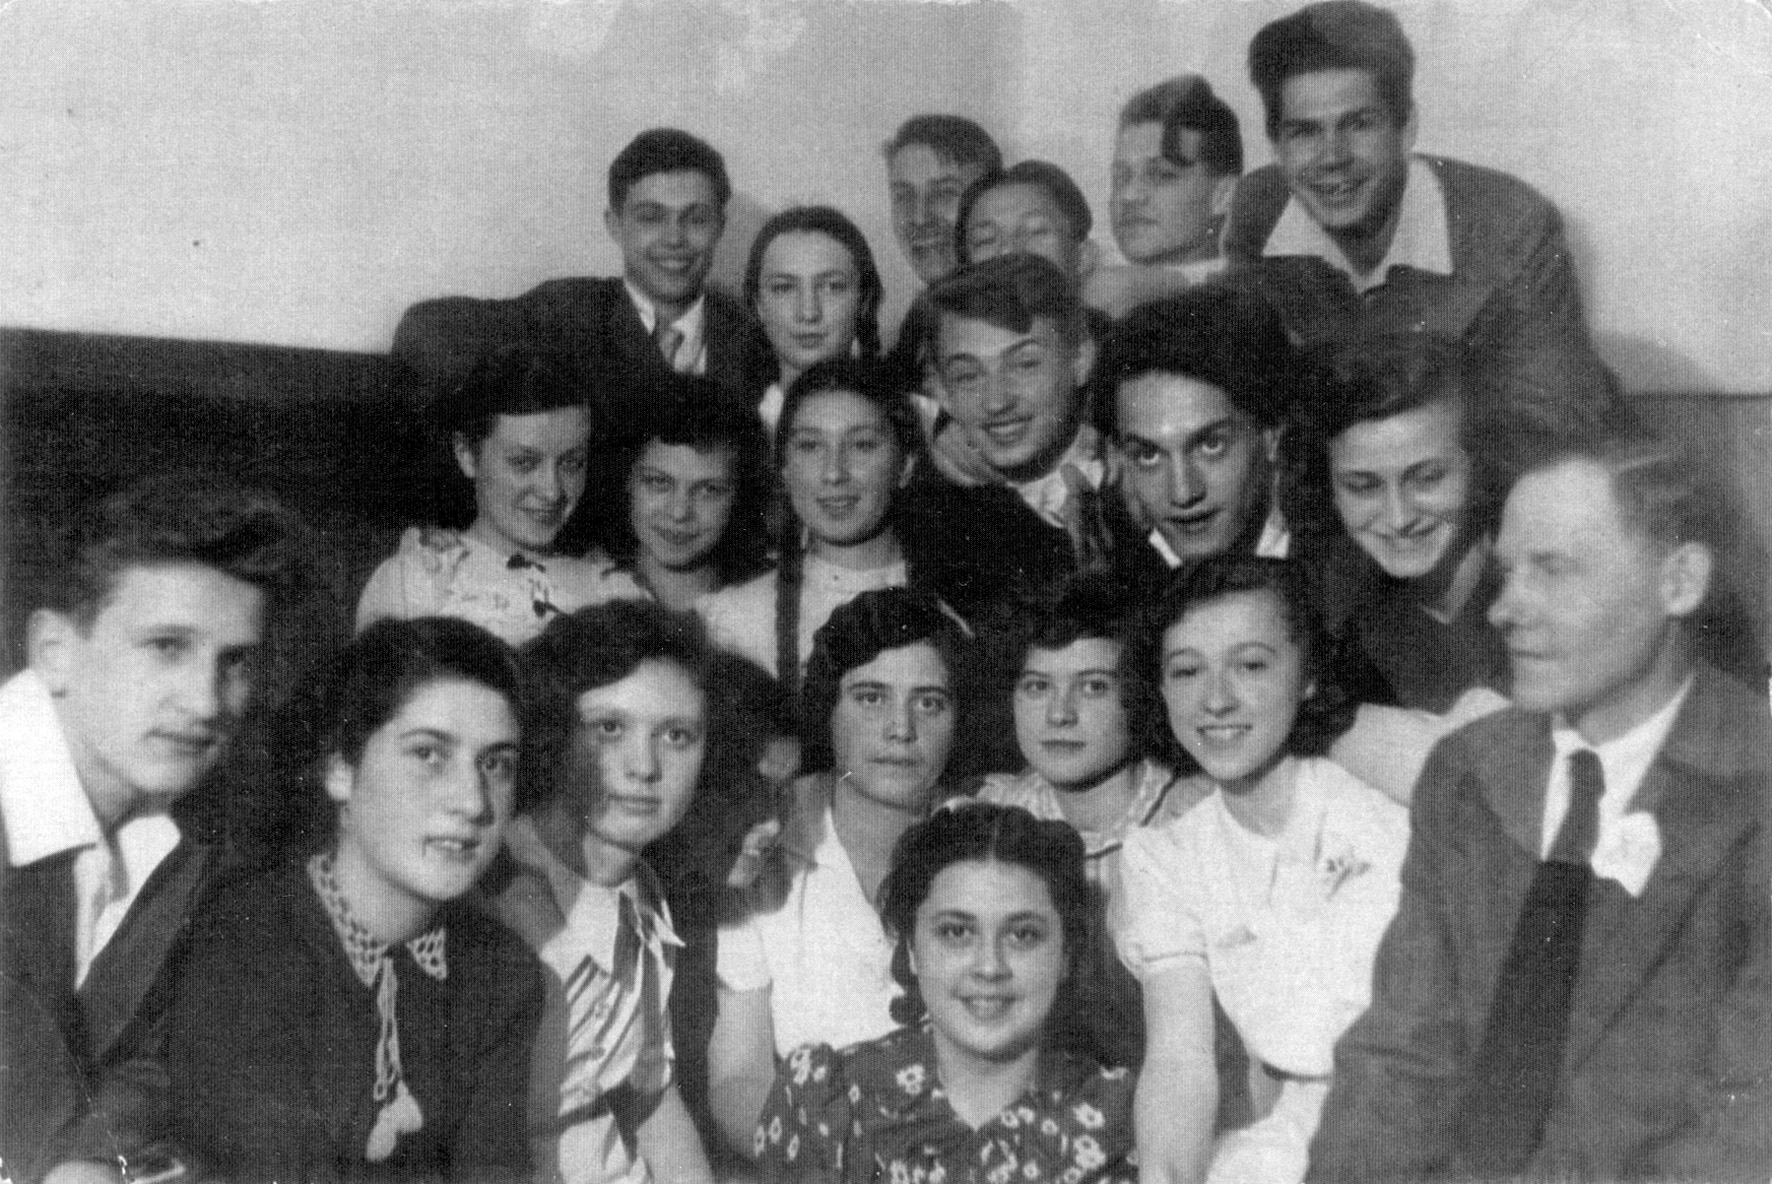
\includegraphics[width=0.5\textwidth]{inc/MalDev}
\end{center}
\begin{center}
    \footnotesize{
    \textbf {Мальчикам и девочкам 1940-х} \\
    (1924 года рождения)
    }
\end{center}

\scriptsize{
\begin{multicols}{2}
    
    \noindent
    К ребятам нашего двора \\
    Пришла не лучшая пора. \\
    \vfill
    \noindent
    Груз годов ведь с плеч не скинешь,\\
    И, куда не поглядишь,\\
    Всюду виден, вроде, фииниш,\\
    И осталось, вроде, шиш! \\
    \vfill
    \noindent
    Только нам, знать, срок не вышел,\\
    Только порох, видно, есть,\\
    Коли вновь мы, братцы, здесь,\\
    Коль мы снова тут, под крышей\\
    Дома номер два дробь шесть.\\
    \vfill
    \noindent
    Откуда шли, шпана дворовая,\\
    Когда пришла пора суровая\\
    Расстаться, шумною толпой\\
    В жизнь, как на праздник~--пей да пой!,--\\
    Ушли веселую шурьбой.\\
    Да каждый со своей судьбой.\\
    \vfill
    \noindent
    Пошли, в цепочку растянувшись,\\
    Один, едва начав, споткнувшись,\\
    Далече не успел уйти\\
    По незавдному пути;\\
    Другой, гляди, взлетел высоко,\\
    А третий ускакал далеко...\\
    \vfill   
    \noindent 
    А мир для всех куда как шире;\\
    В иных домах на нашец жизни ткань:\\
    То~-- шелк с парчей, то~-- просто дрянь!\\
    То планов дрезких грамадье,\\
    То только старое тряпье.\\
    \vfill
    \noindent
    Но жизнь~-- от Бога и надолго.\\
    И не забыть бы, братцы, долга\\
    За нами~-- тем, кто нас родил,\\
    Да тем, кто раньше уходил.\\
    Но не в прекрасную страну,\\
    А на проклятую войну.\\
    \vfill
    \noindent
    Утащила злая баба,\\
    Уложила в поле сдуру\\
    Твоео братишку Абу,\\
    Моего братана Юру,\\
    Сколько было их~-- не счесть!\\
    Всех помянем благородно,\\
    Отдадим посмертно честь!\\
    \vfill
    \noindent
    С непкурытой головою,\\
    То ли лысой, то ль седою,\\
    Постоим да помолчим.\\
    А потом уж прокричим\\
    Из последних сил, что есть,\\
    Славу дому два дробь шесть!\\
\end{multicols}
\vspace*{-5mm}
\raggedleft{С. И. Д. (Дивильковский С. И.), 2010 г.

}
}


\restoregeometry


\mainmatter % это включает нумерацию глав и секций в документе ниже



%\backmatter %% Здесь заканчивается нумерованная часть документа и начинаются ссылки и
            %% заключение



\appendix   % Тут идут приложения

\chapter{}

\section*{Из <<Вундеркинда>> №1. 1947г.}

Первая сессия верховного совета ССД была открыта 31 марта 1947г. в Большом Дворце Красного Уголка. сессию открыл старейший депутат т. Прейс.

Выбрав Председателя, депутаты выслушали отчет Председателя Центральной избирательной комиссии т.  Горностаева и приступили к выборам Президента.

Голосованием было установлено, что на пост Президента ССД избран тов. Дивильковский.

Затем т. Прейс зачитал список Министров, а те, в свою очередь, выбрали Председателя совета Министров: тов. Гриневского.

Утвержден также Гимн ССД (поется на мотив из Девушки моей мечты.):

\vfill

{\itshape

Славься, славься Государство наше,

Самая прекрасная страна.

Ты всех стран сильнее, могучее и краше

круглый год в тебе стоит весна!

\vfill

Славься, славься ССД во веки~--

Демократия в тебе сильна.

Здесь живут свободно человеки,

Круглый год в тебе стоит весна!!

\vfill

В ССД вся власть в руках народа,

Много в нем закусок и вина.

в ССД господствует свобода,

В ССД всегда стоит весна!!!

}

\newgeometry{top=7mm,left=5mm,right=5mm,bottom=5mm}

\section*{Из <<Вундеркинда>> №2. 1947г.}

\noindent
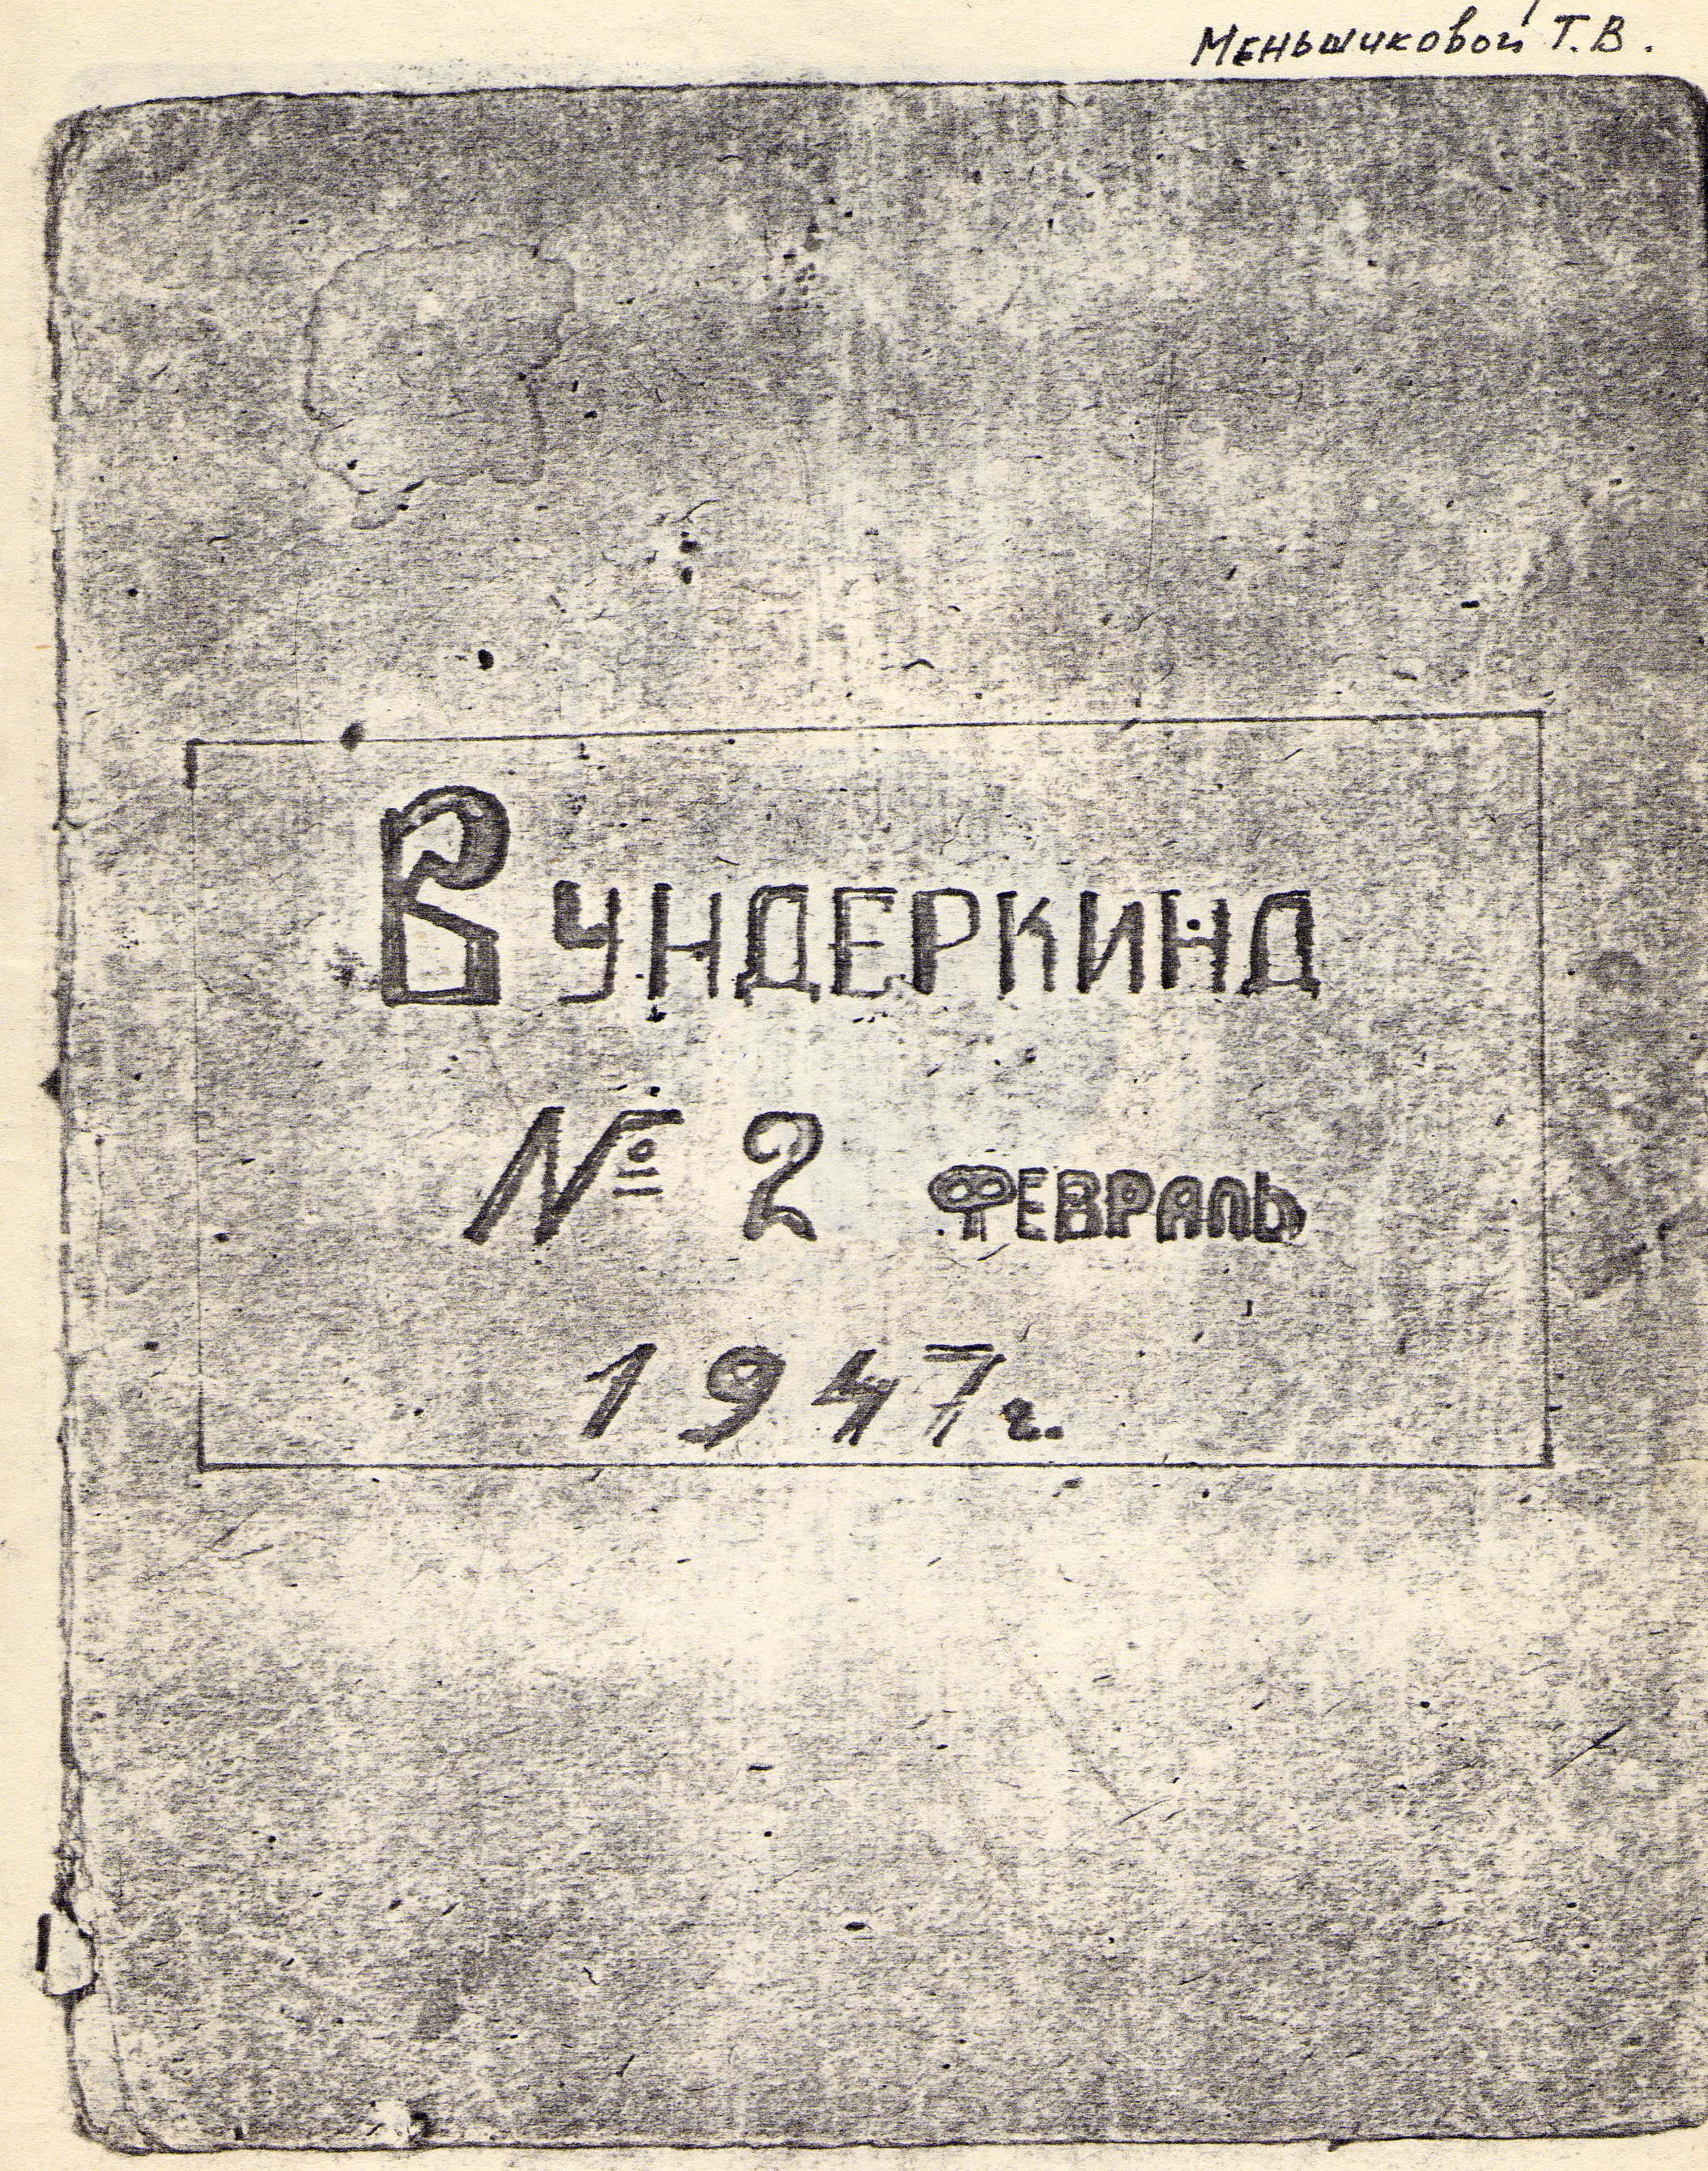
\includegraphics[width=\textwidth]{inc/Vynd/Vynd001}

\newpage

\noindent
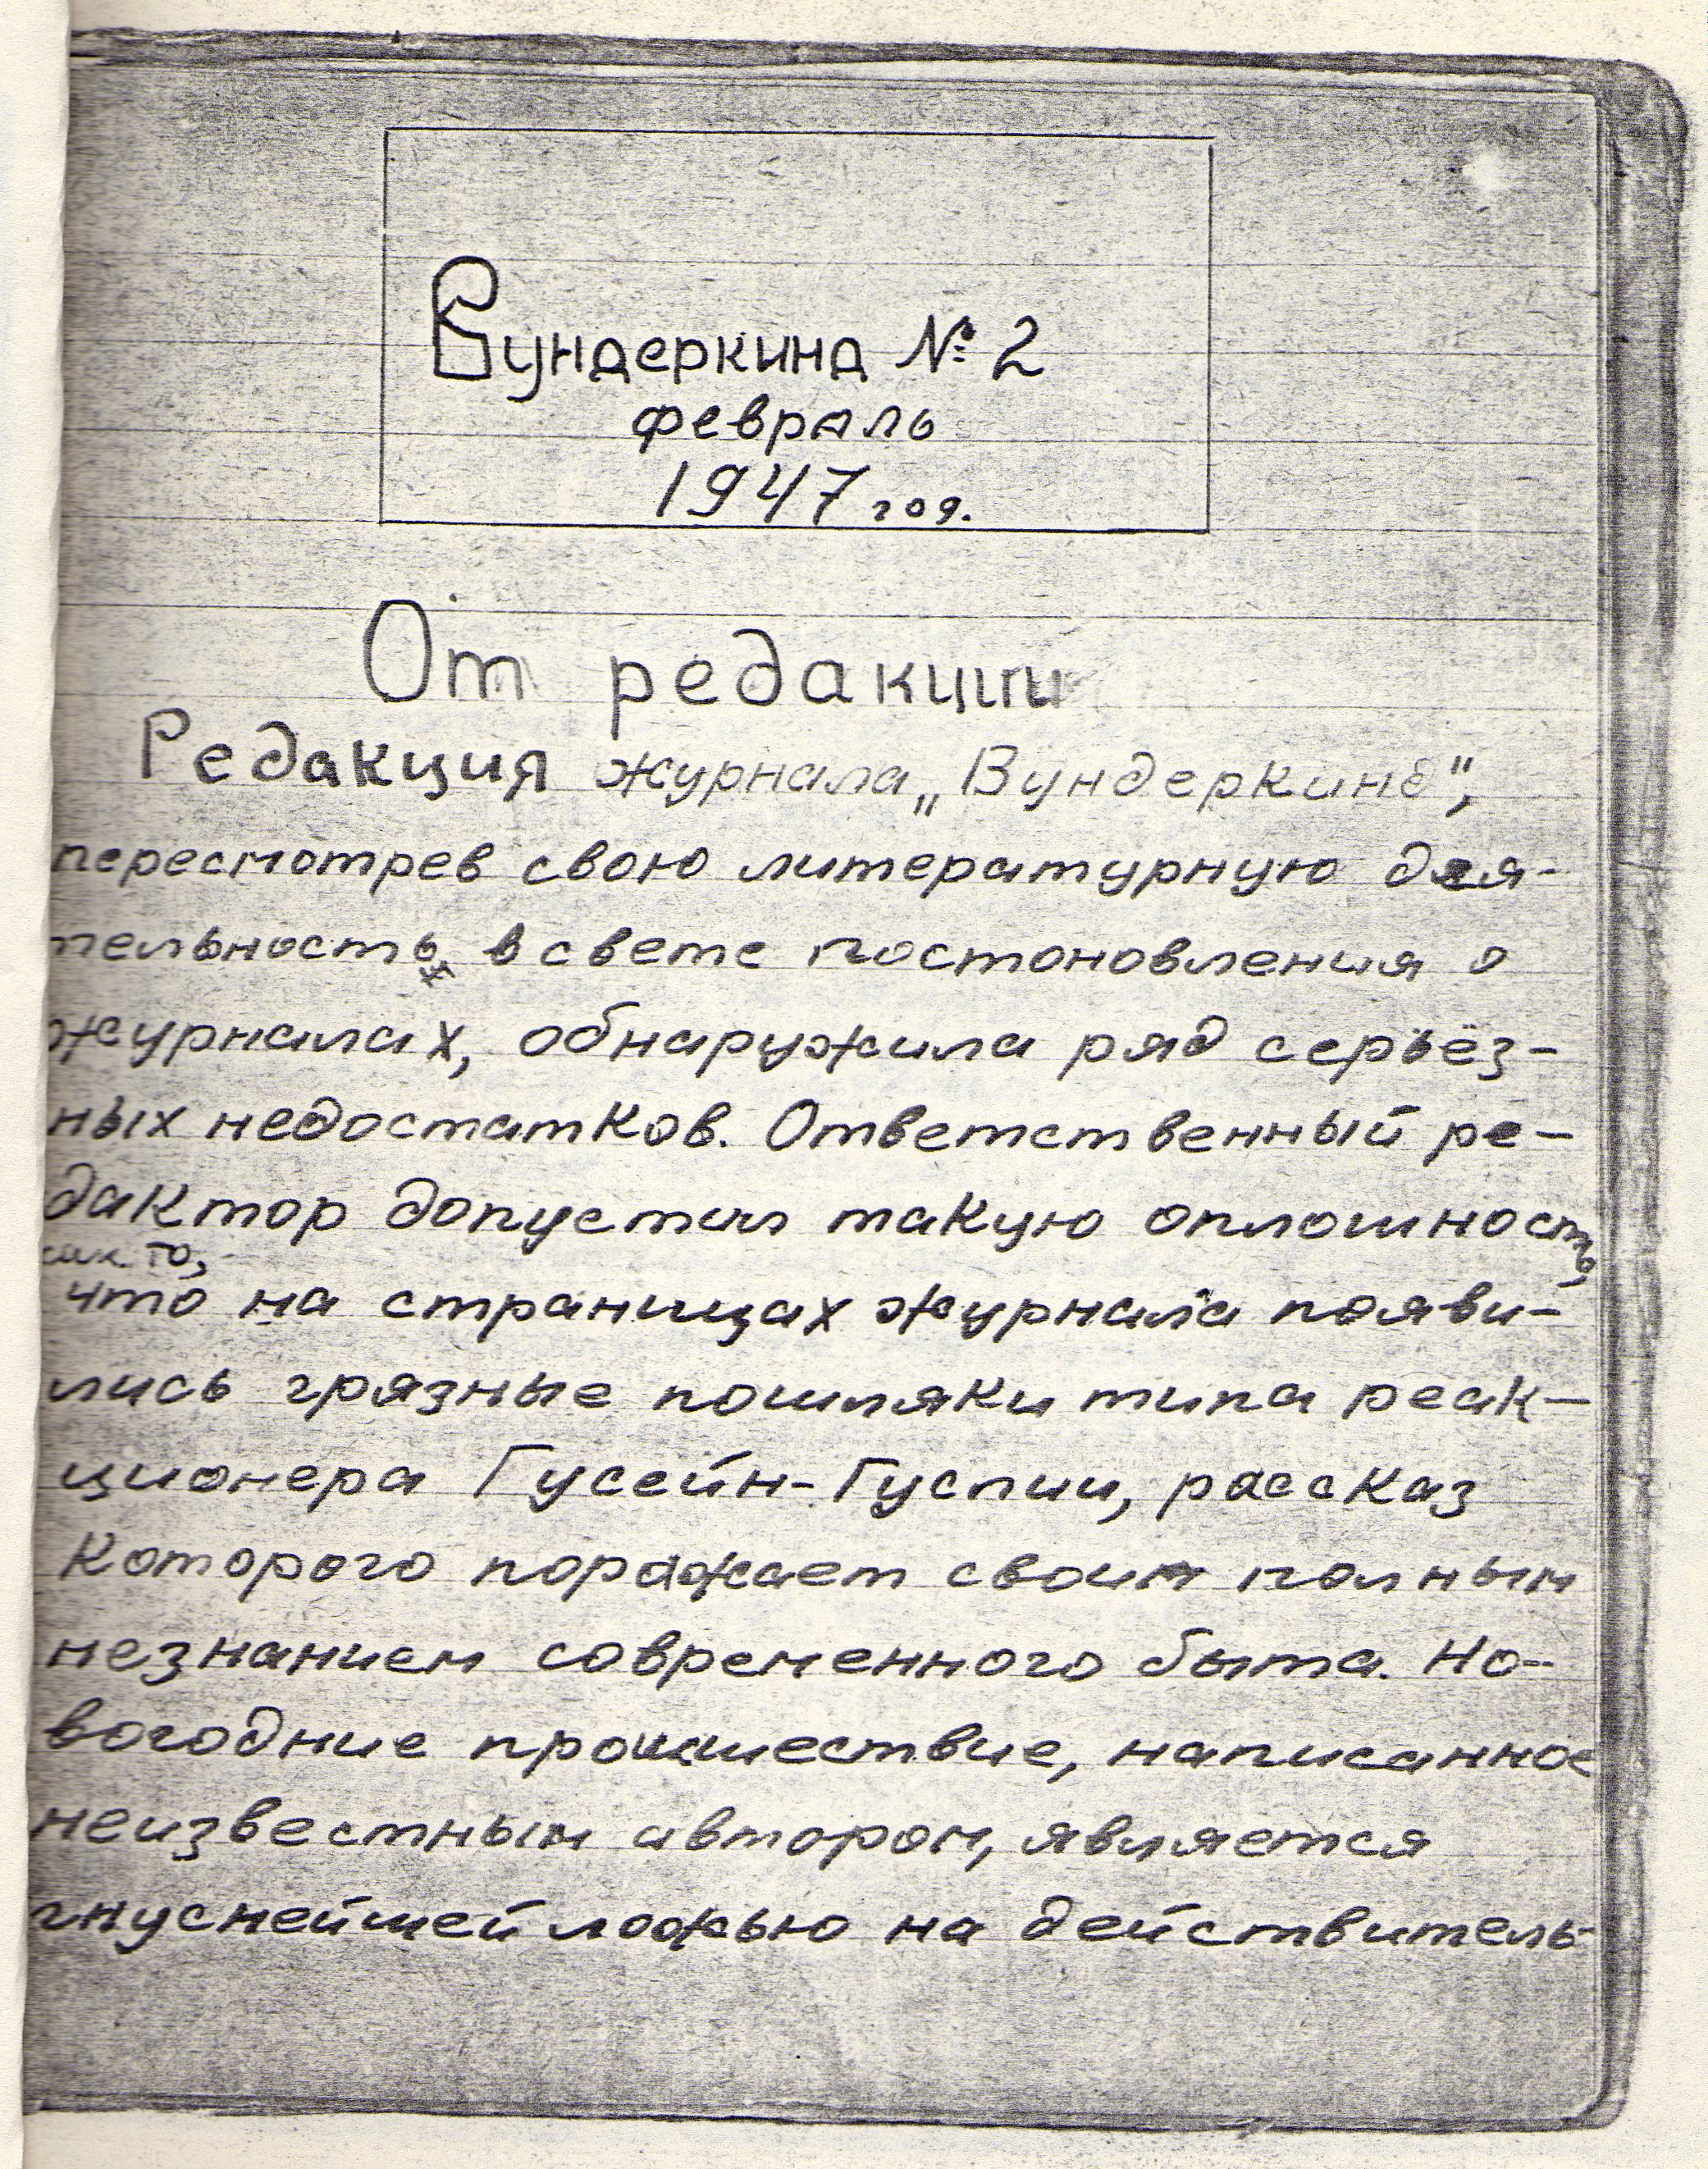
\includegraphics[width=\textwidth]{inc/Vynd/Vynd002}

\noindent
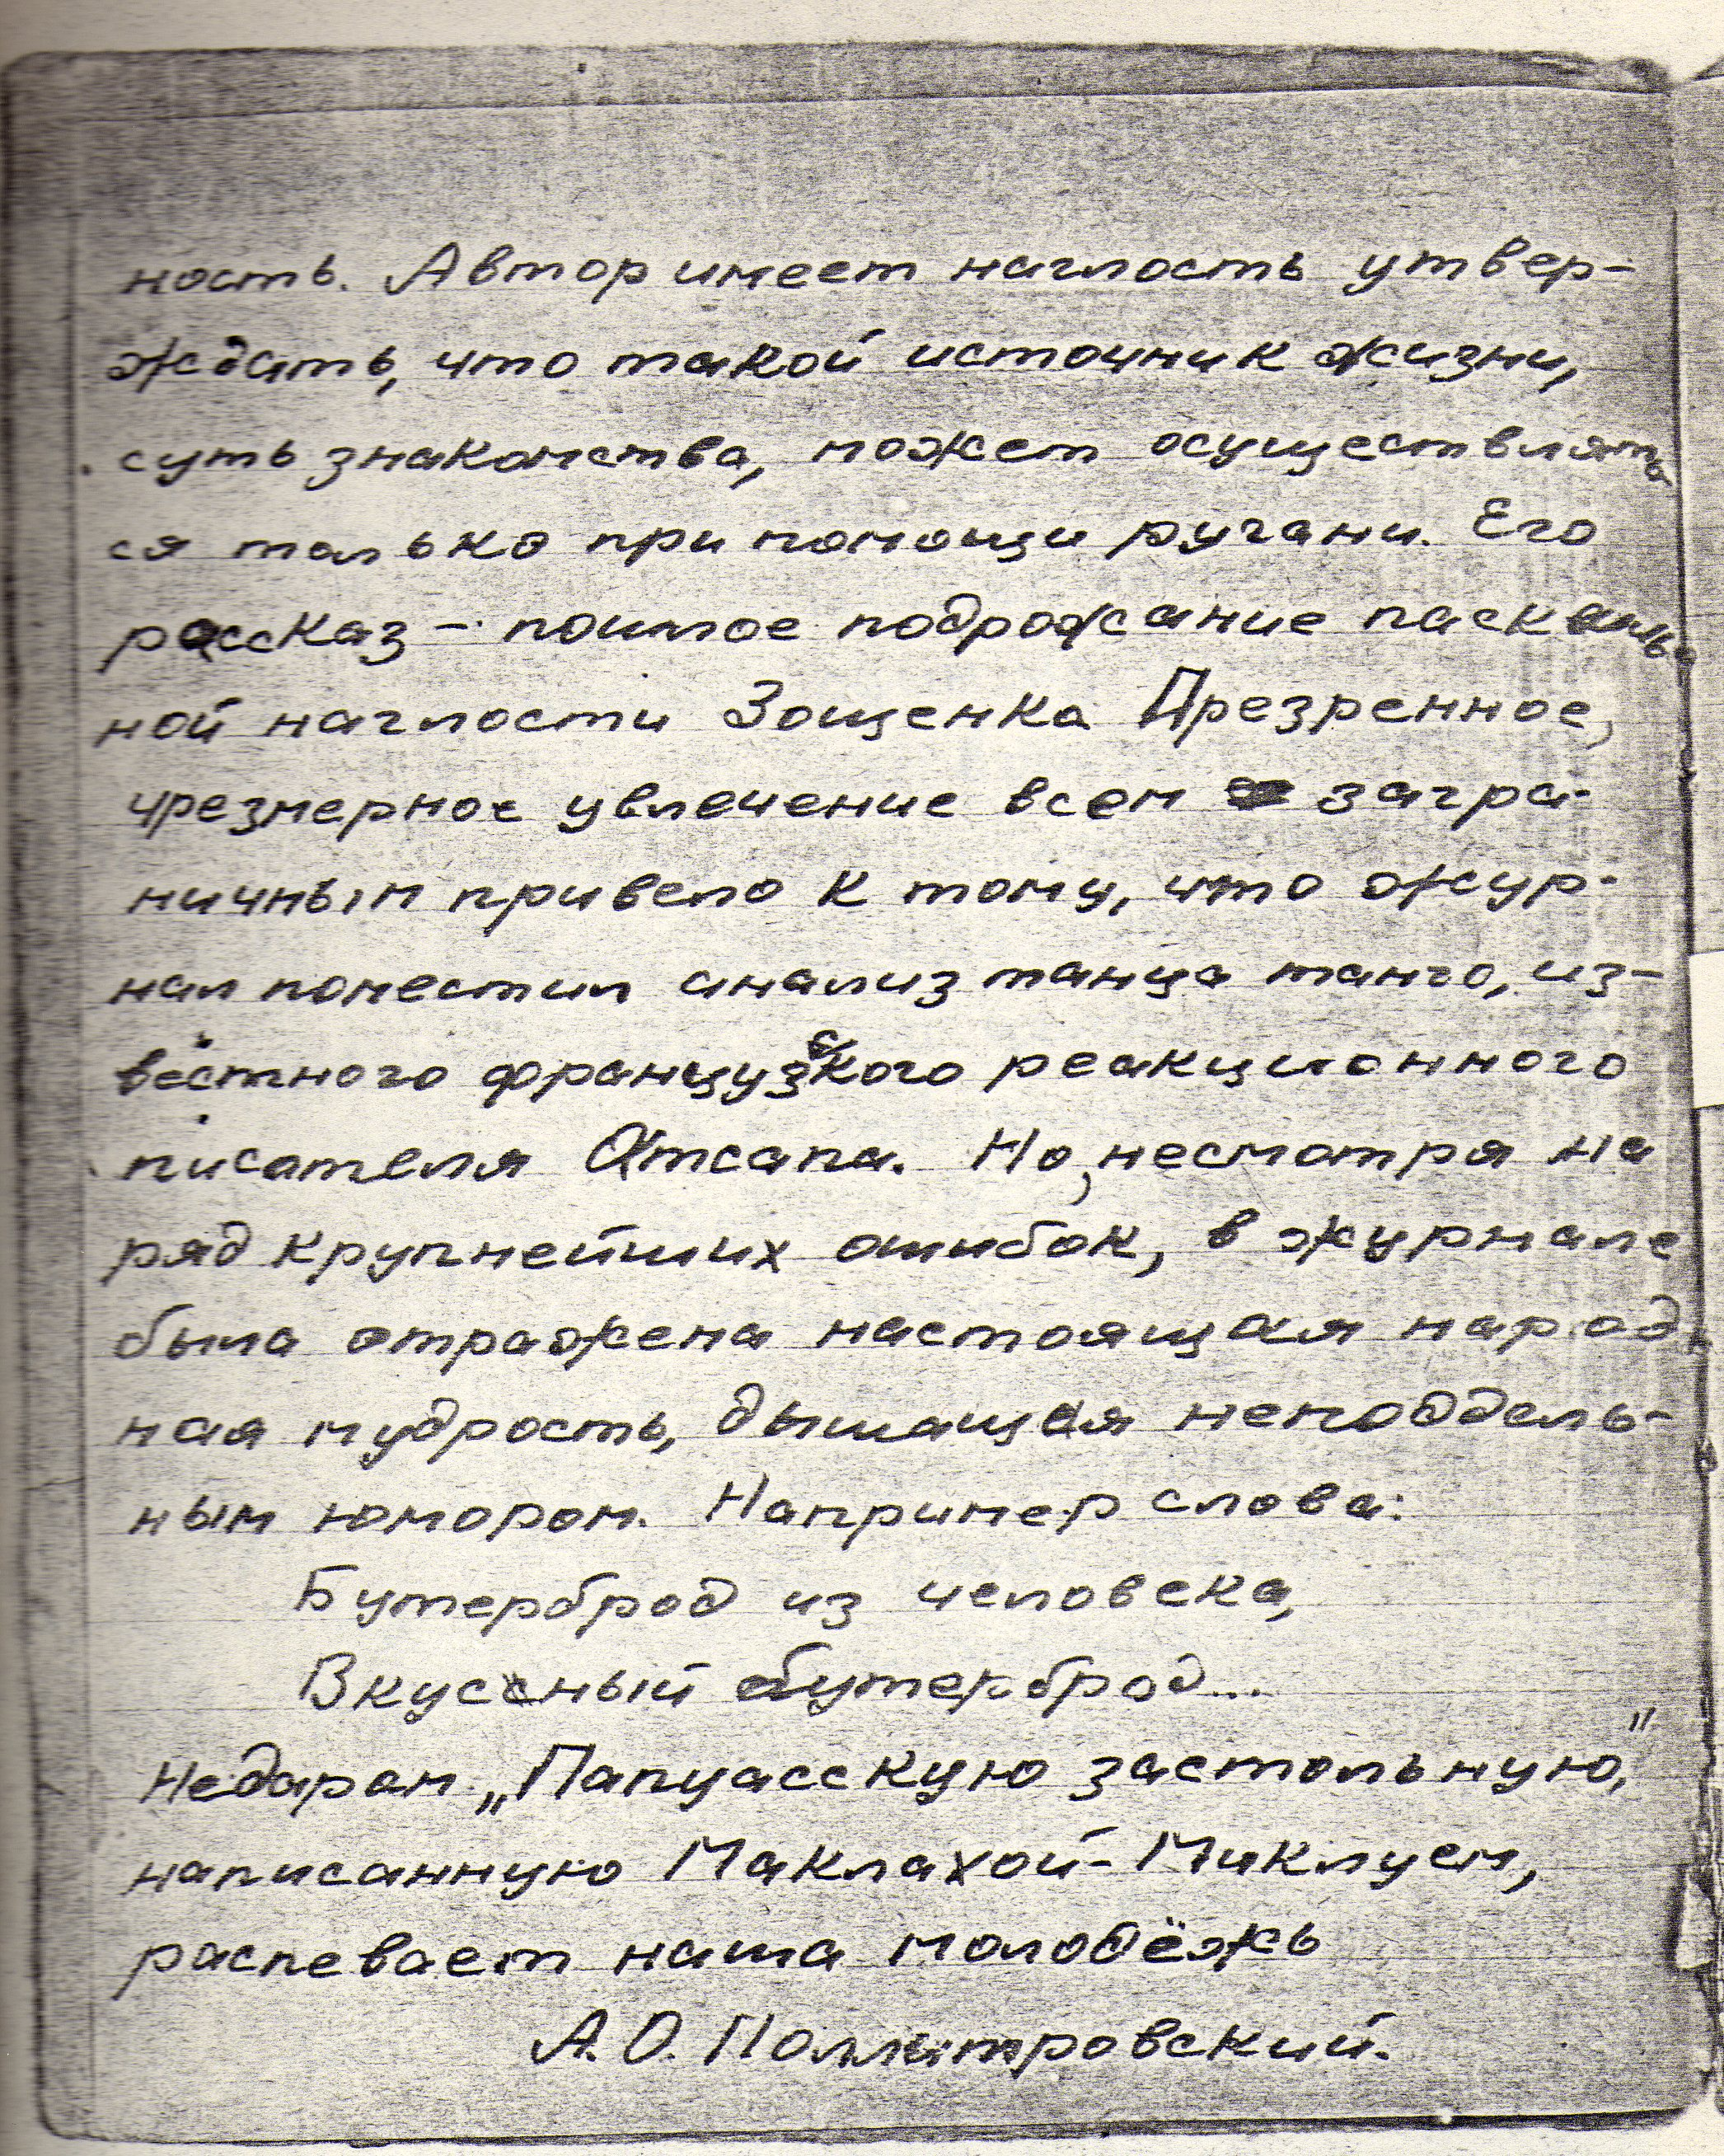
\includegraphics[width=\textwidth]{inc/Vynd/Vynd003}

\newpage


\noindent
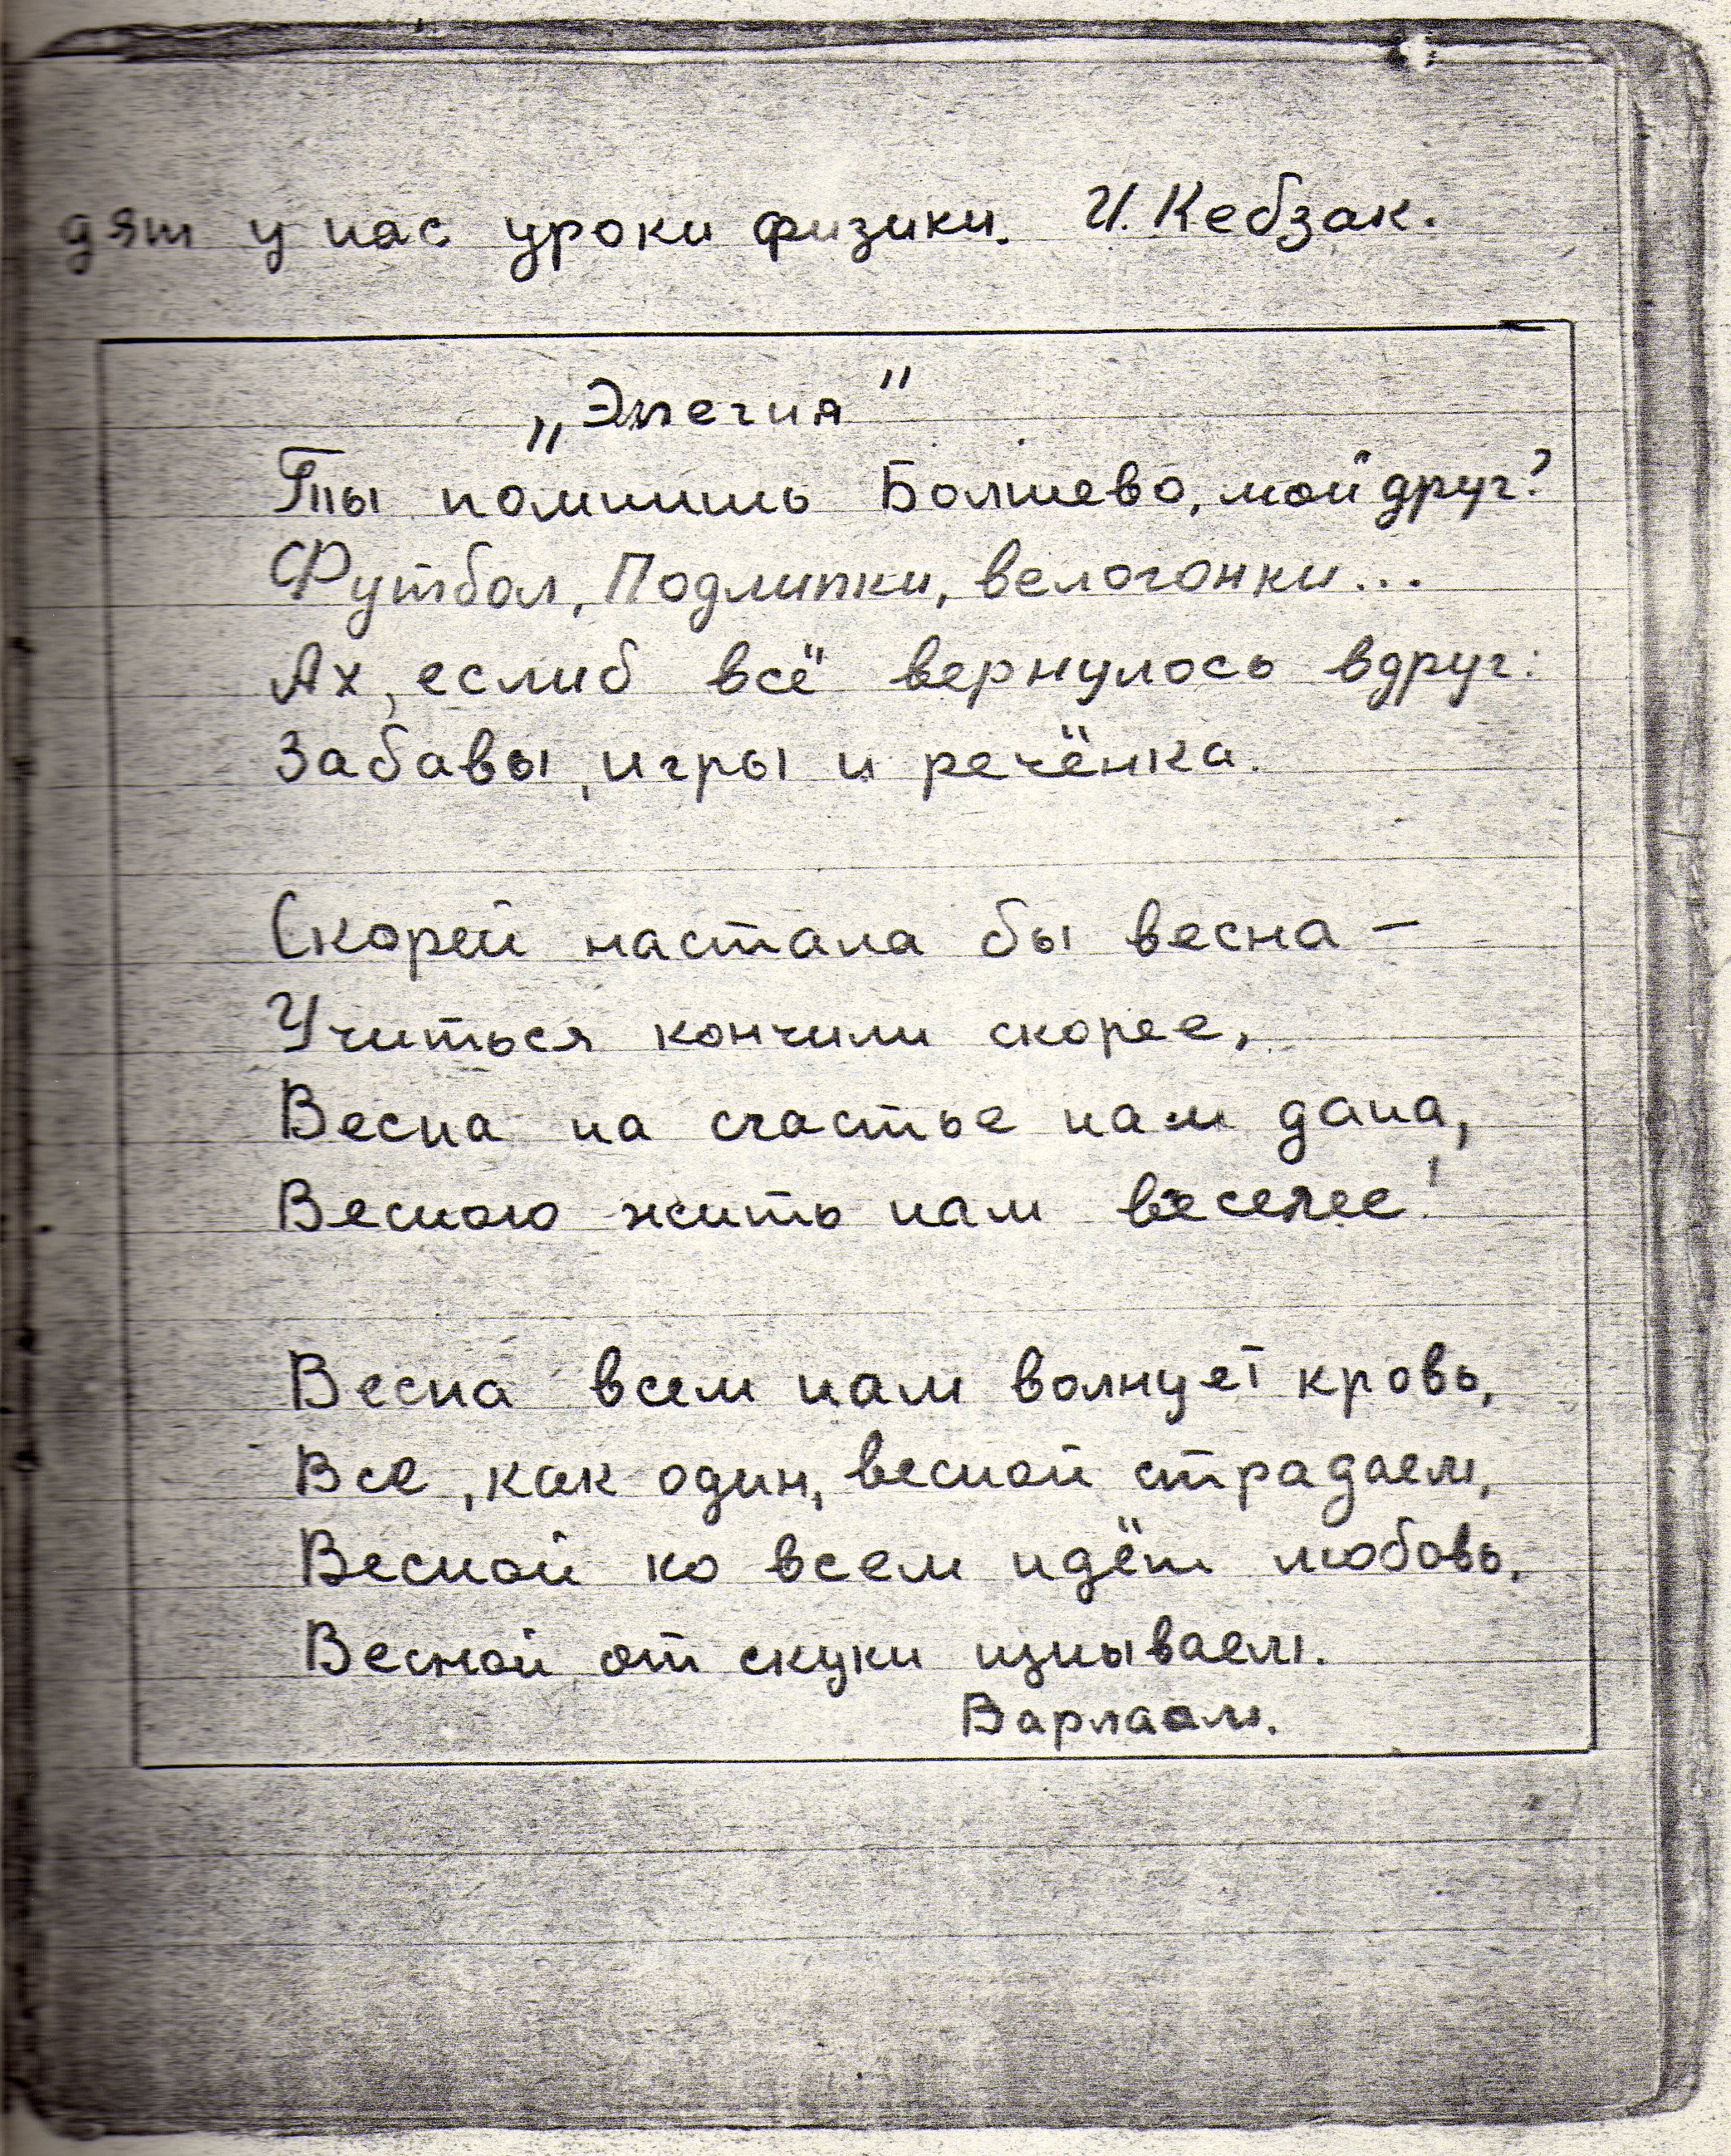
\includegraphics[width=\textwidth]{inc/Vynd/Vynd004}

\noindent
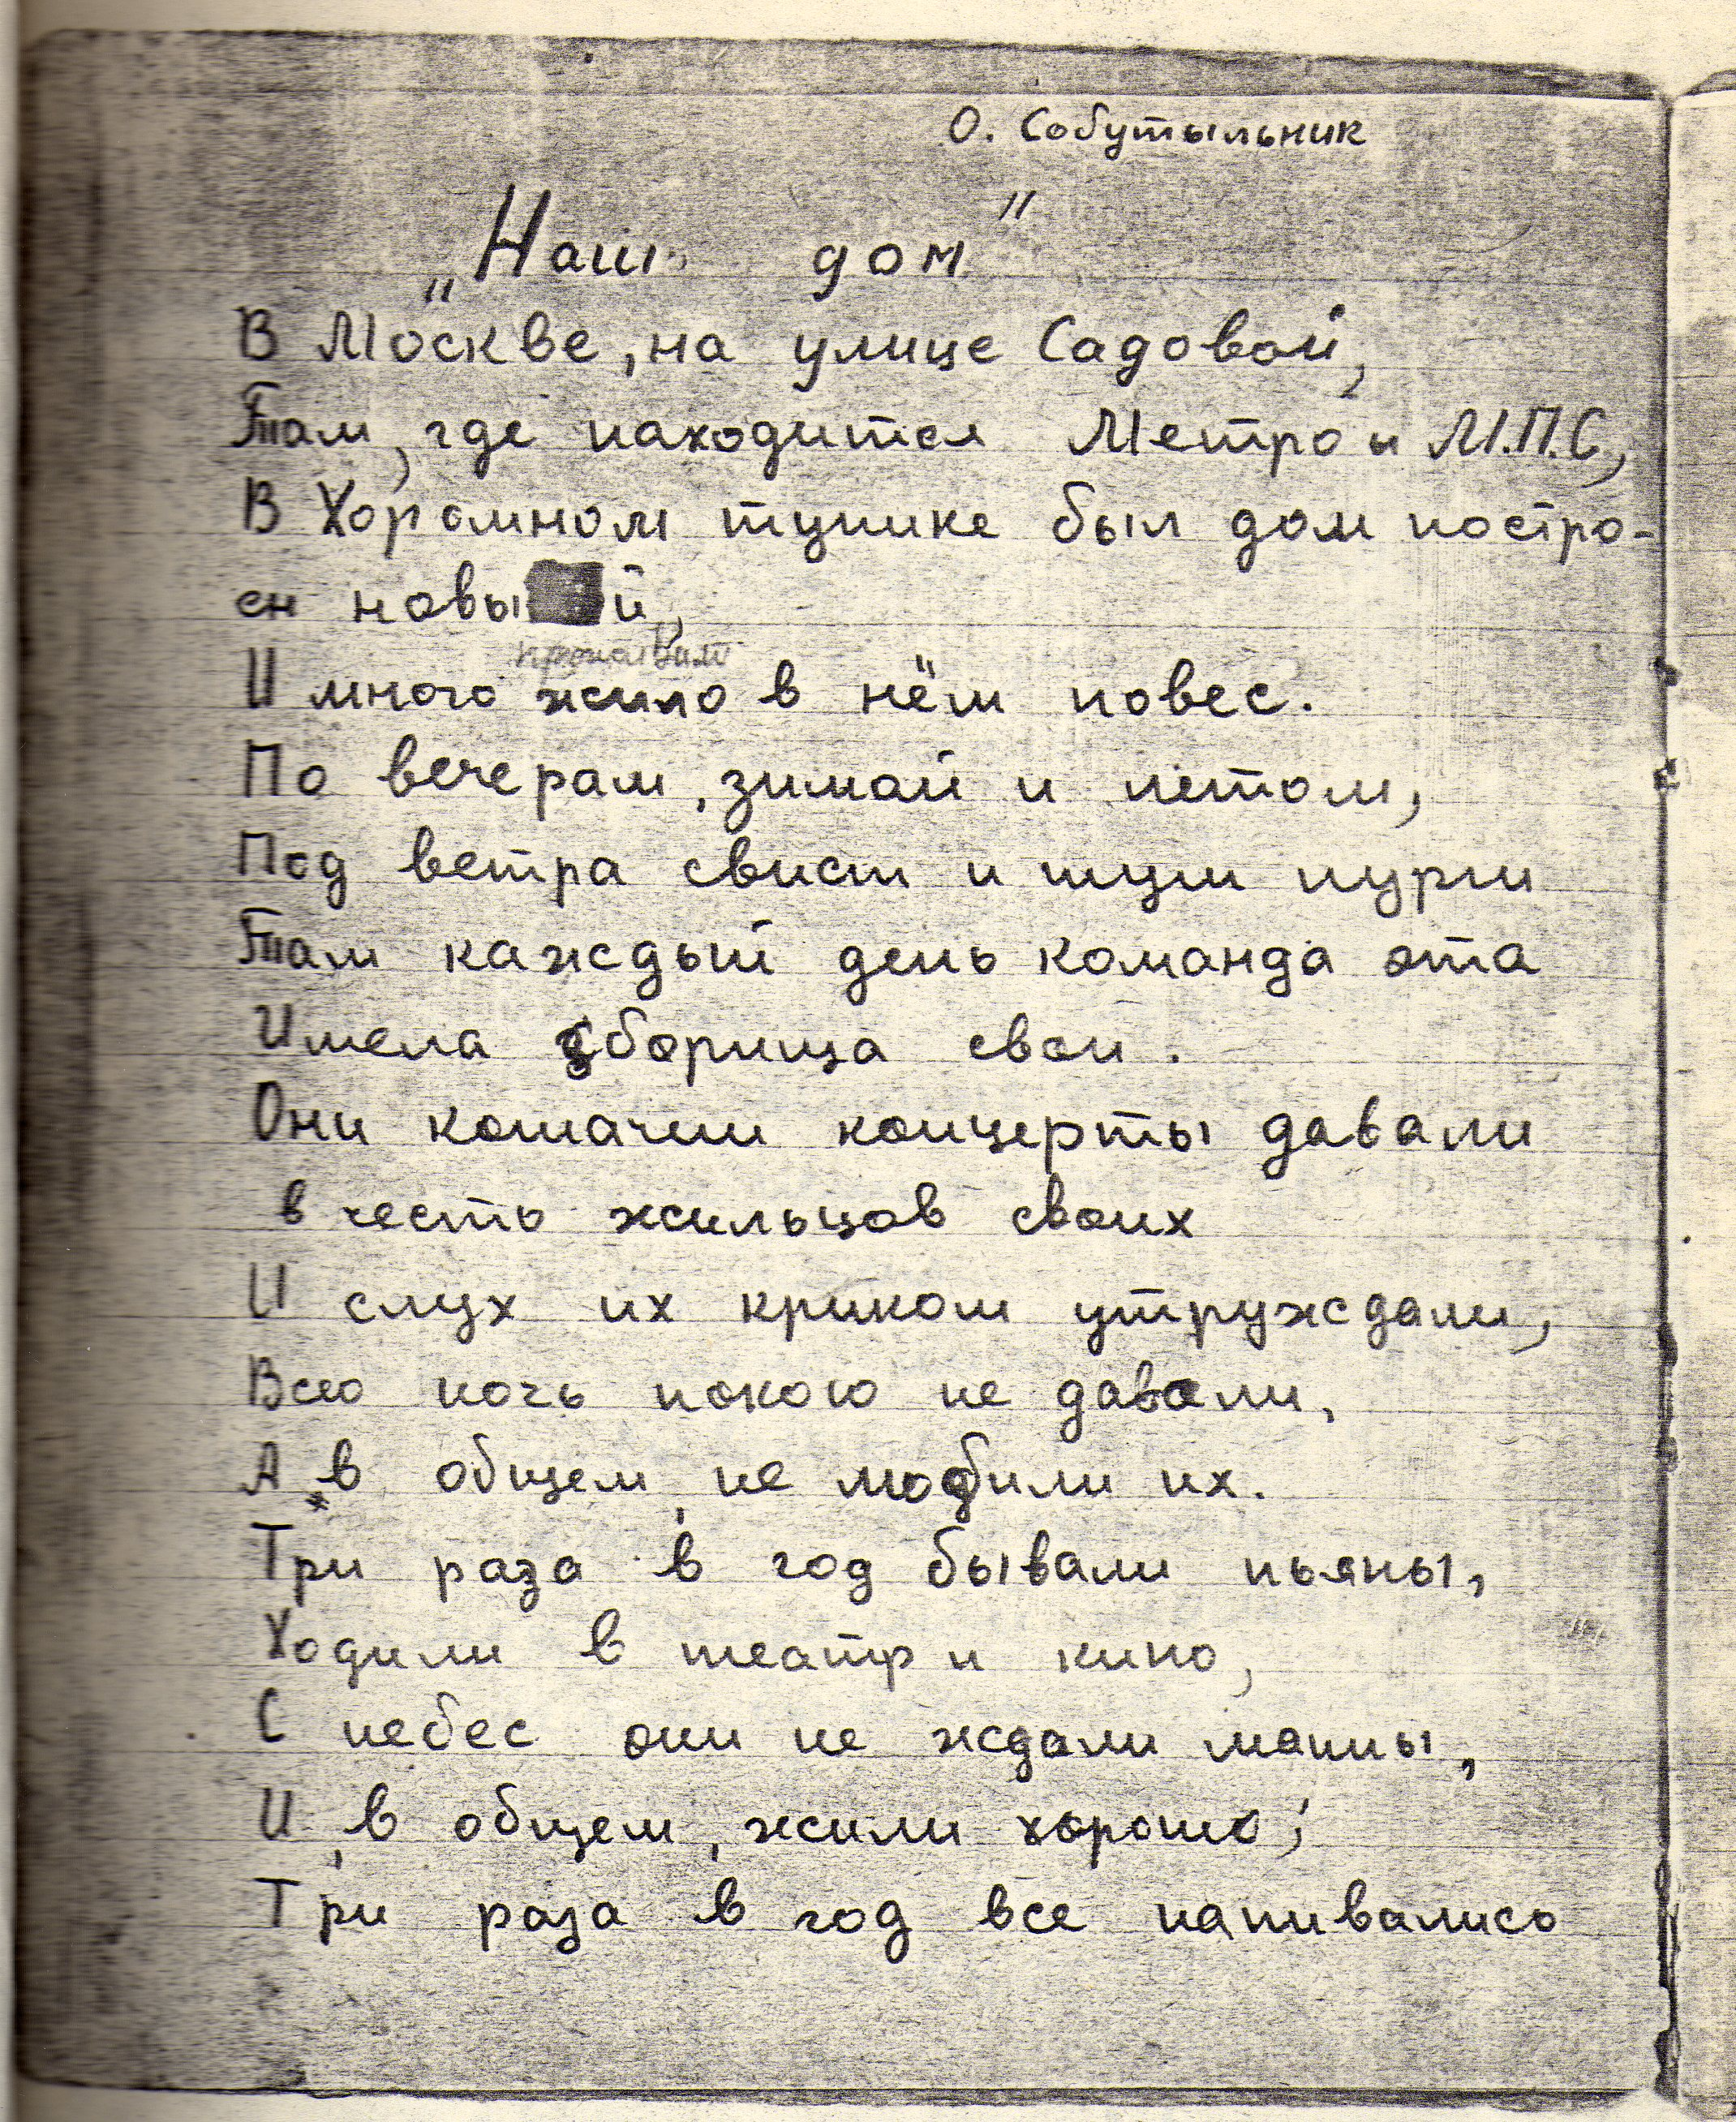
\includegraphics[width=\textwidth]{inc/Vynd/Vynd005}

\noindent
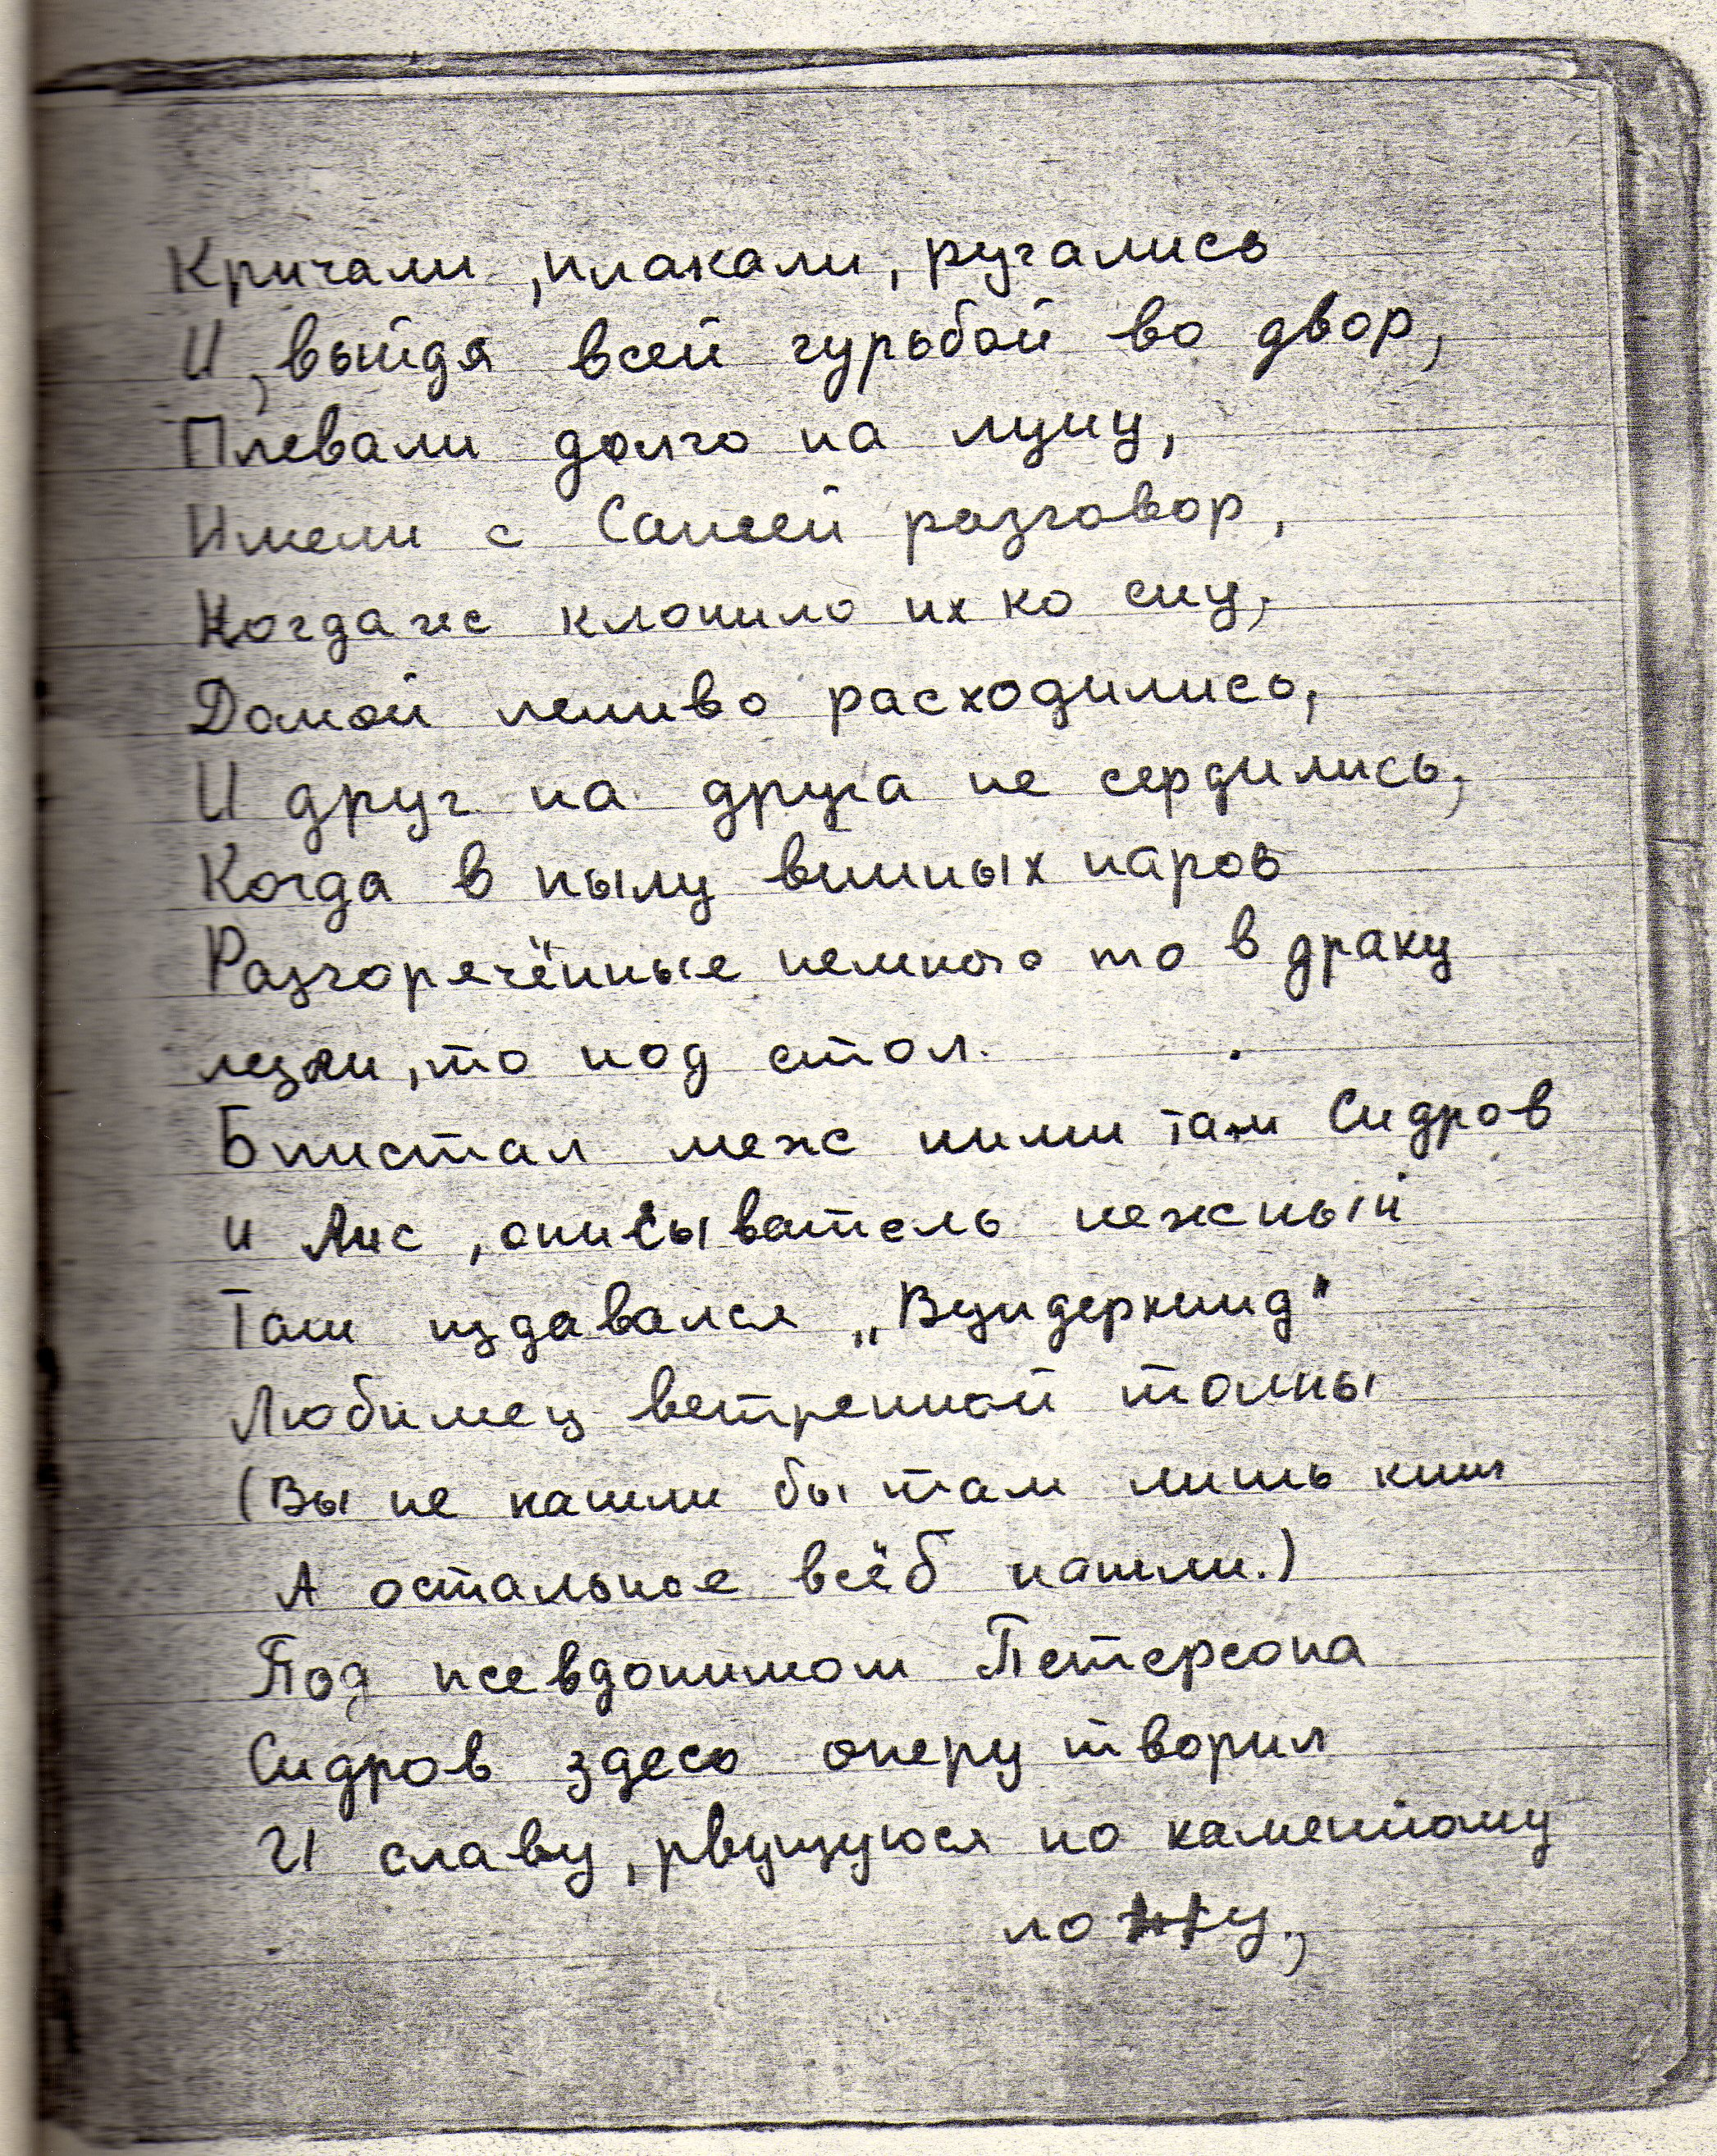
\includegraphics[width=\textwidth]{inc/Vynd/Vynd006}

\noindent
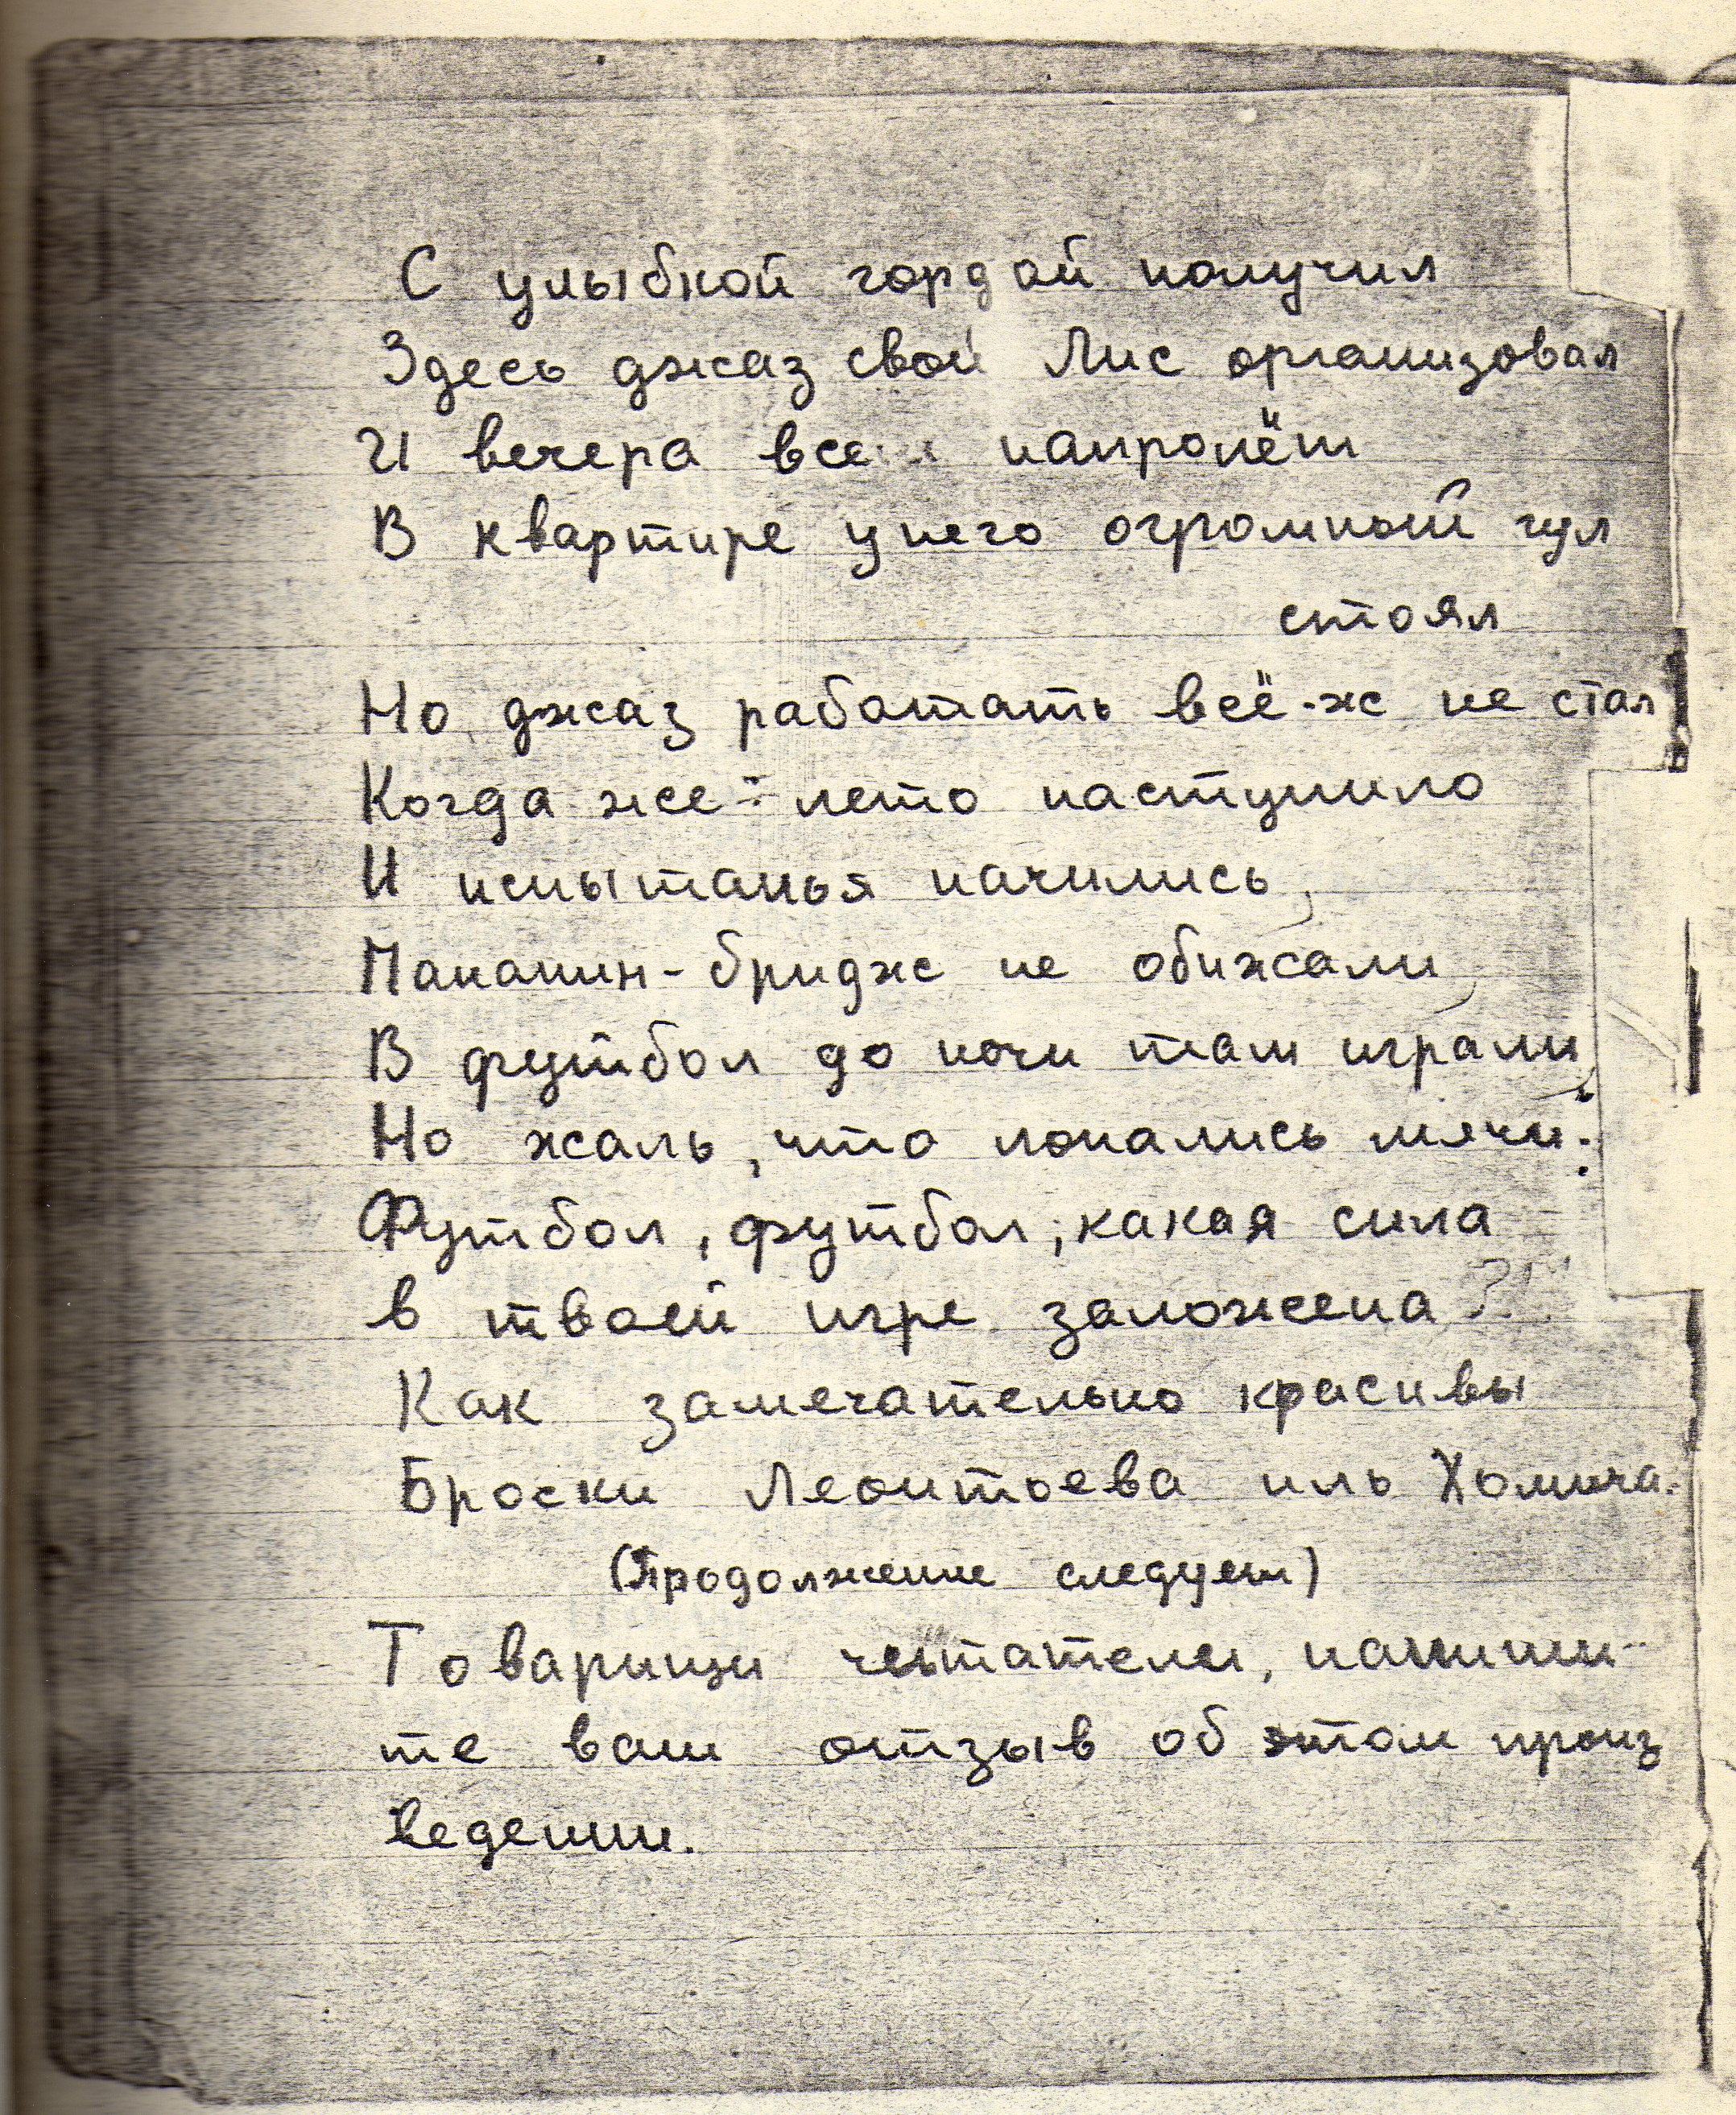
\includegraphics[width=\textwidth]{inc/Vynd/Vynd007}

\noindent
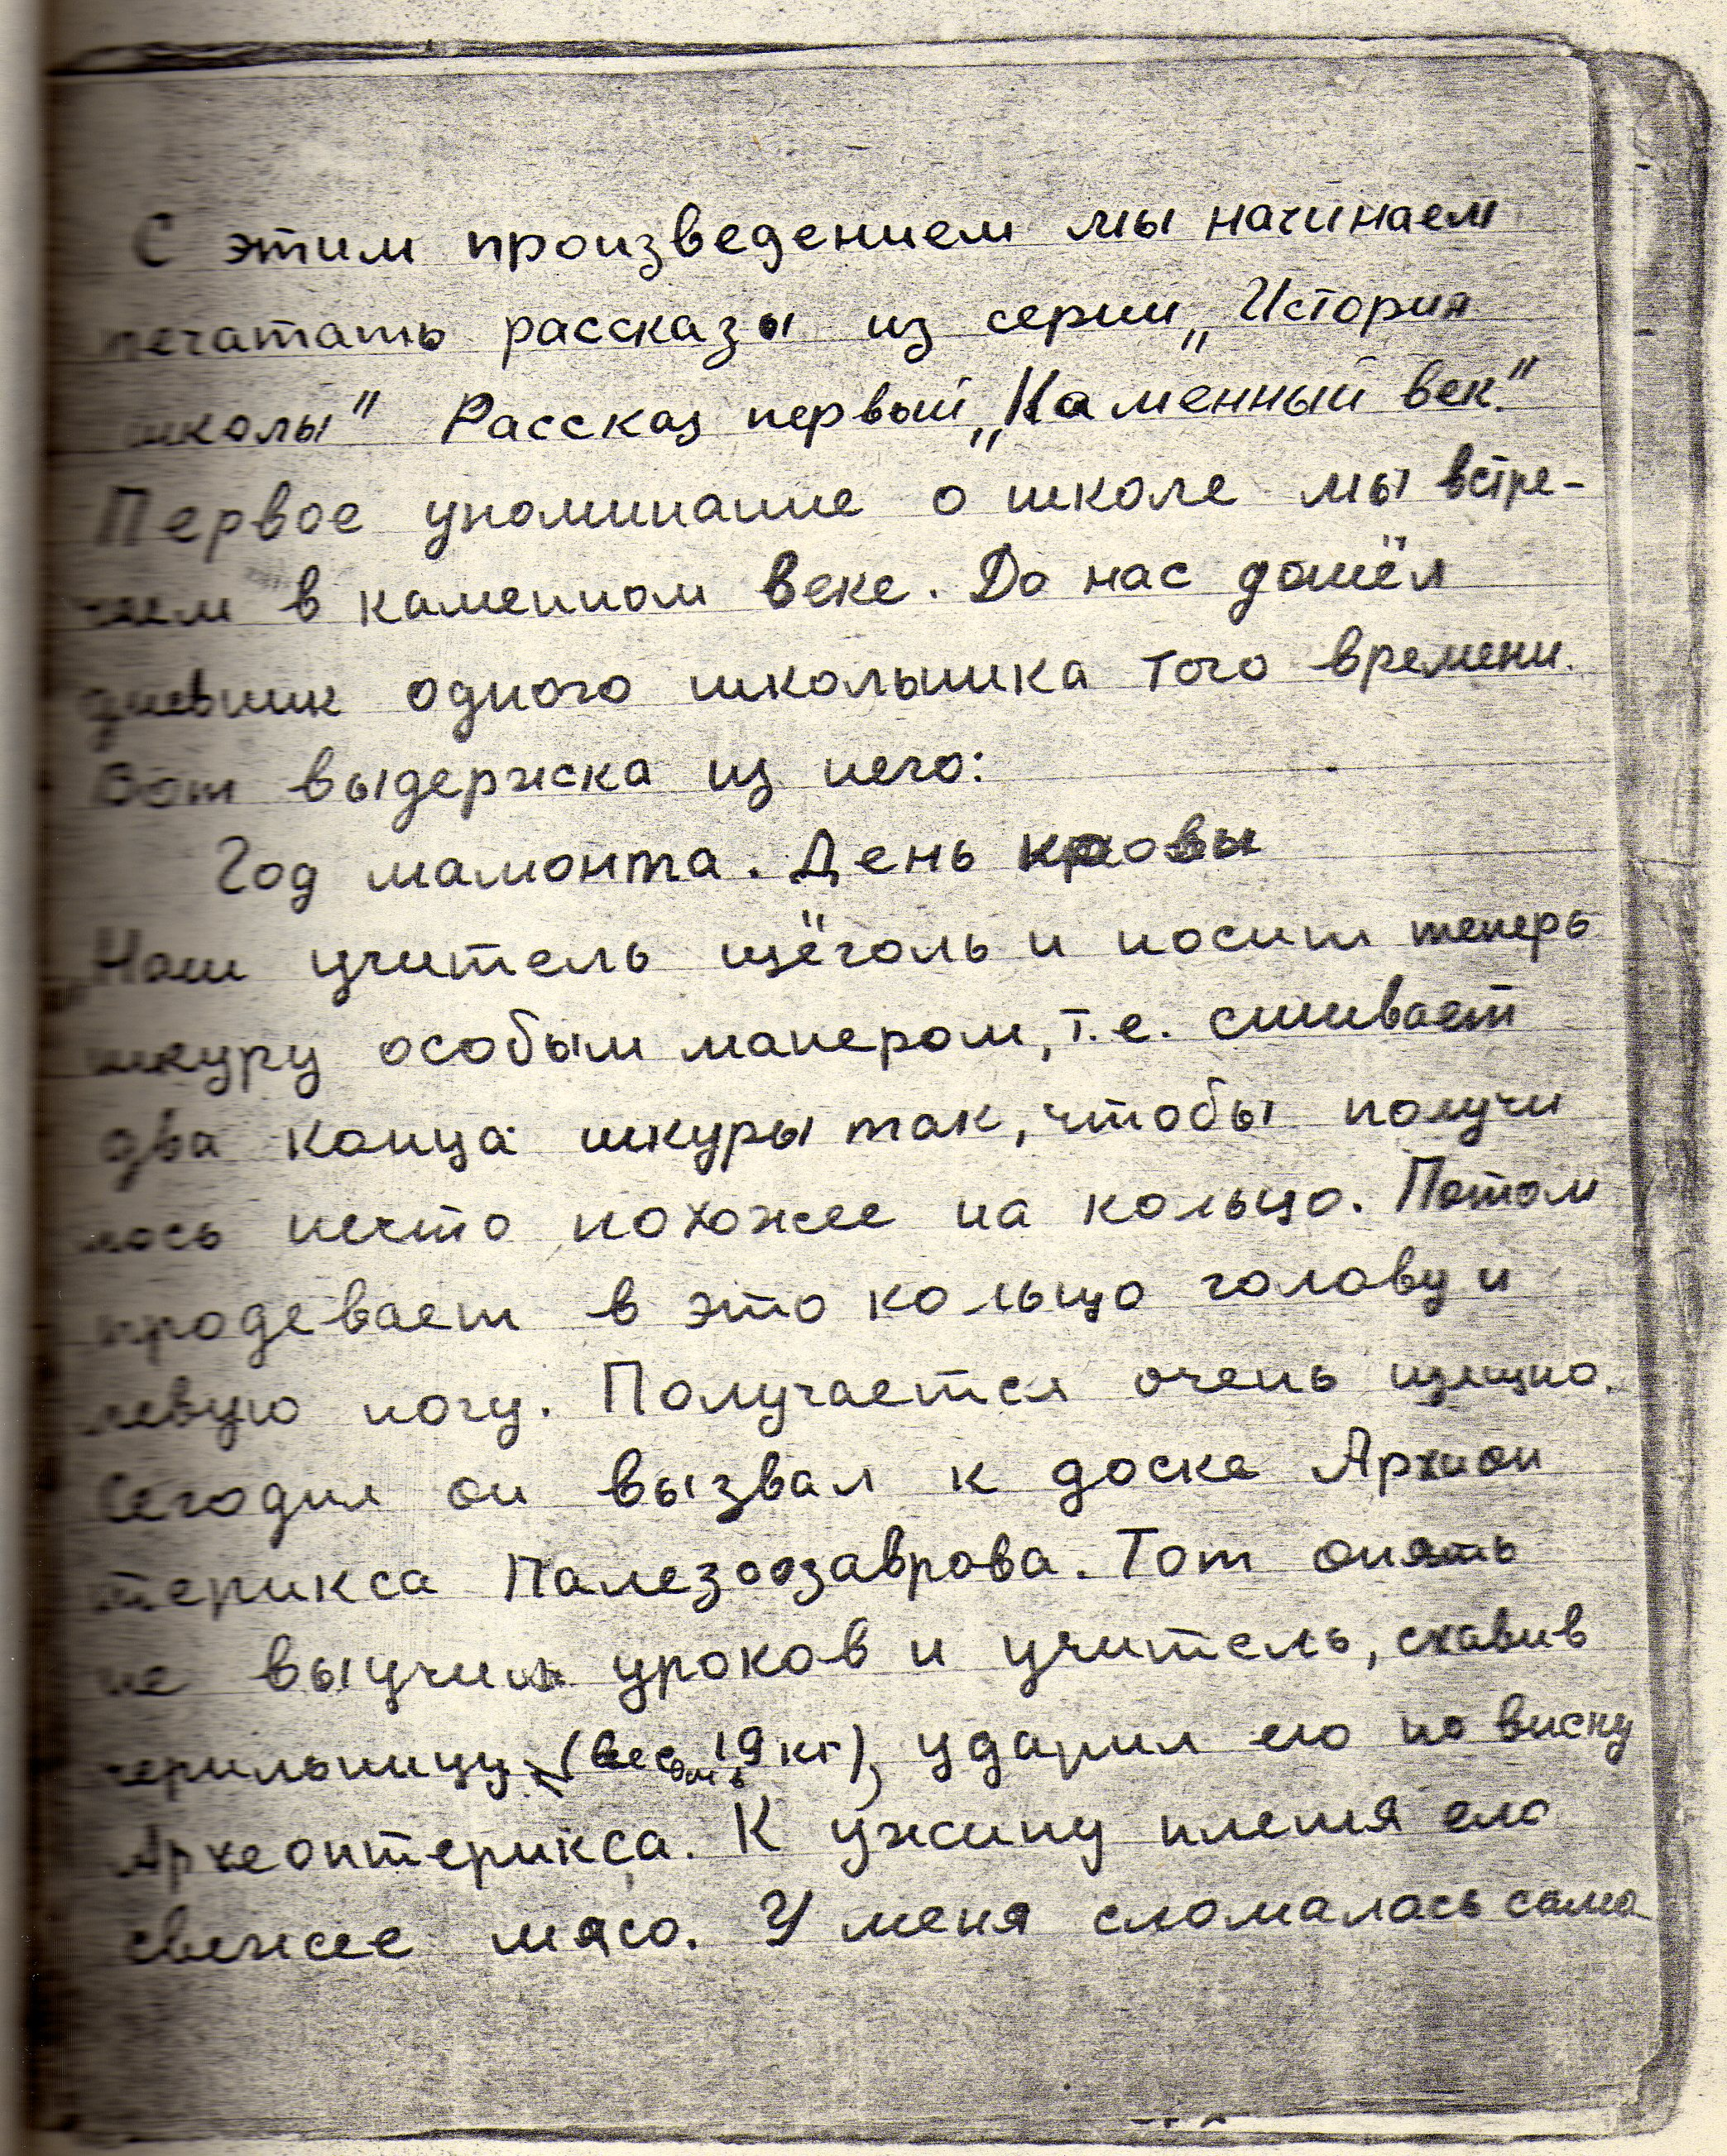
\includegraphics[width=\textwidth]{inc/Vynd/Vynd008}

\newpage

\noindent
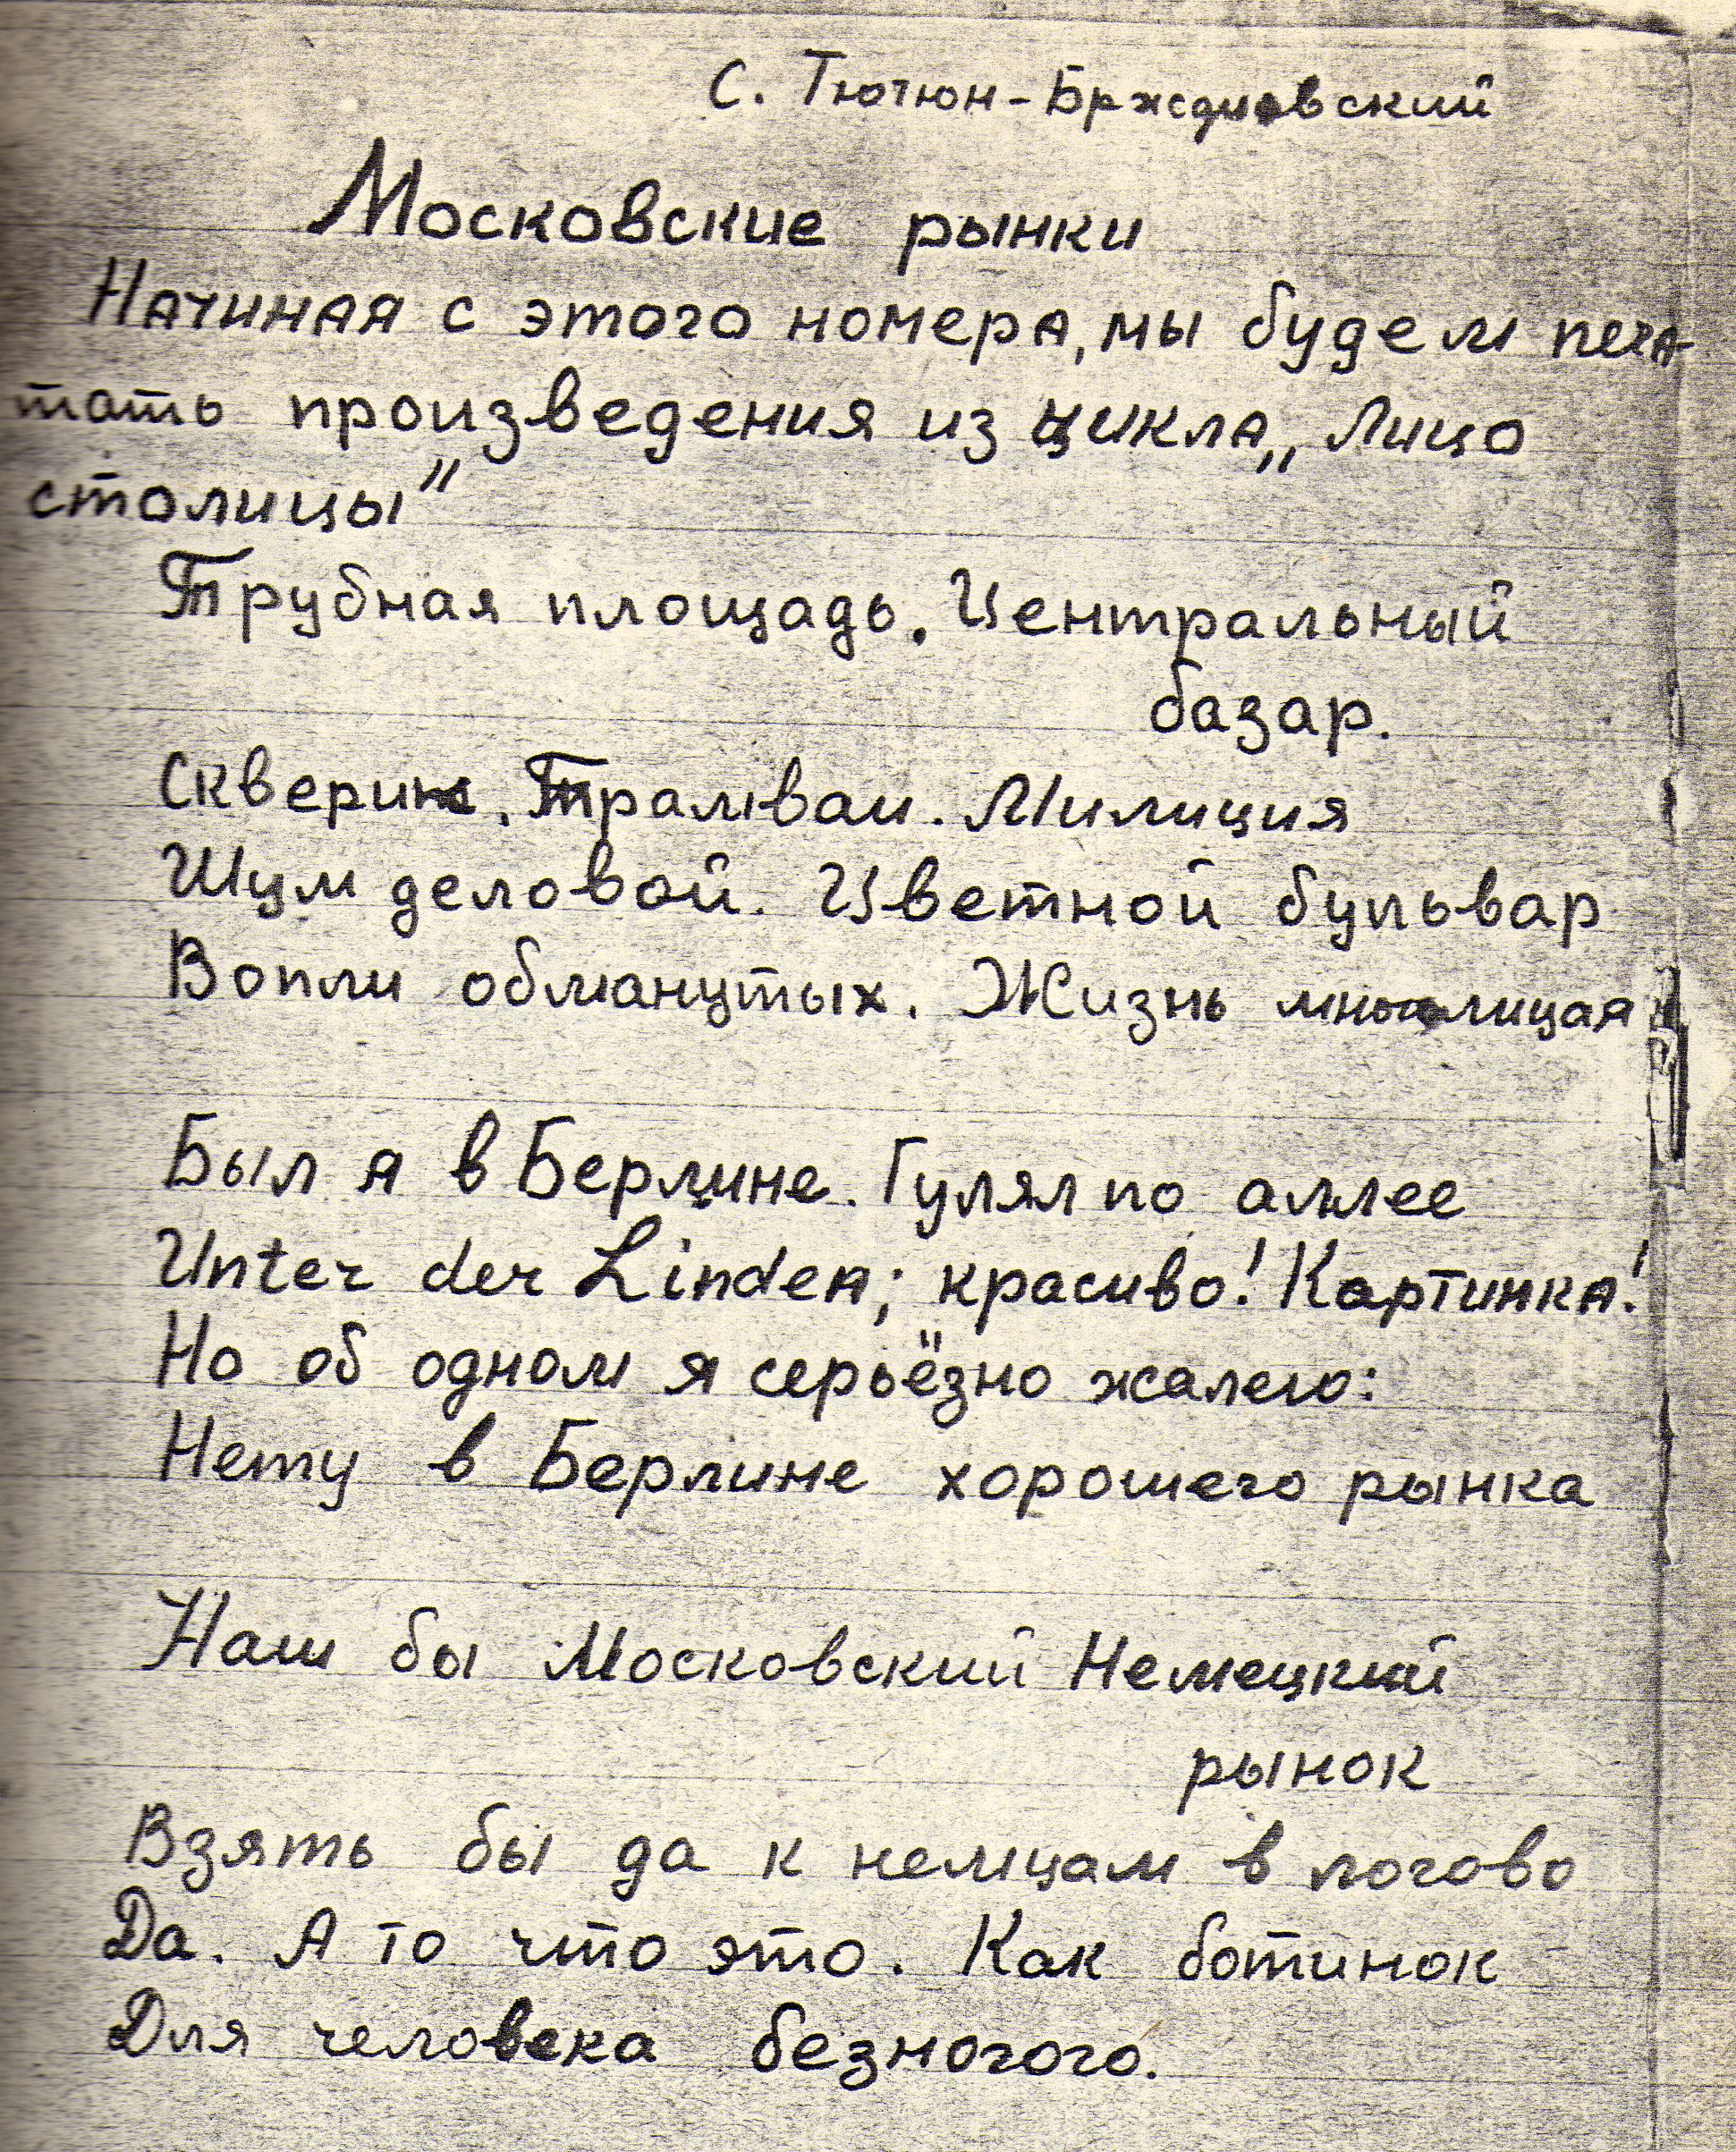
\includegraphics[width=\textwidth]{inc/Vynd/Vynd009}

\noindent
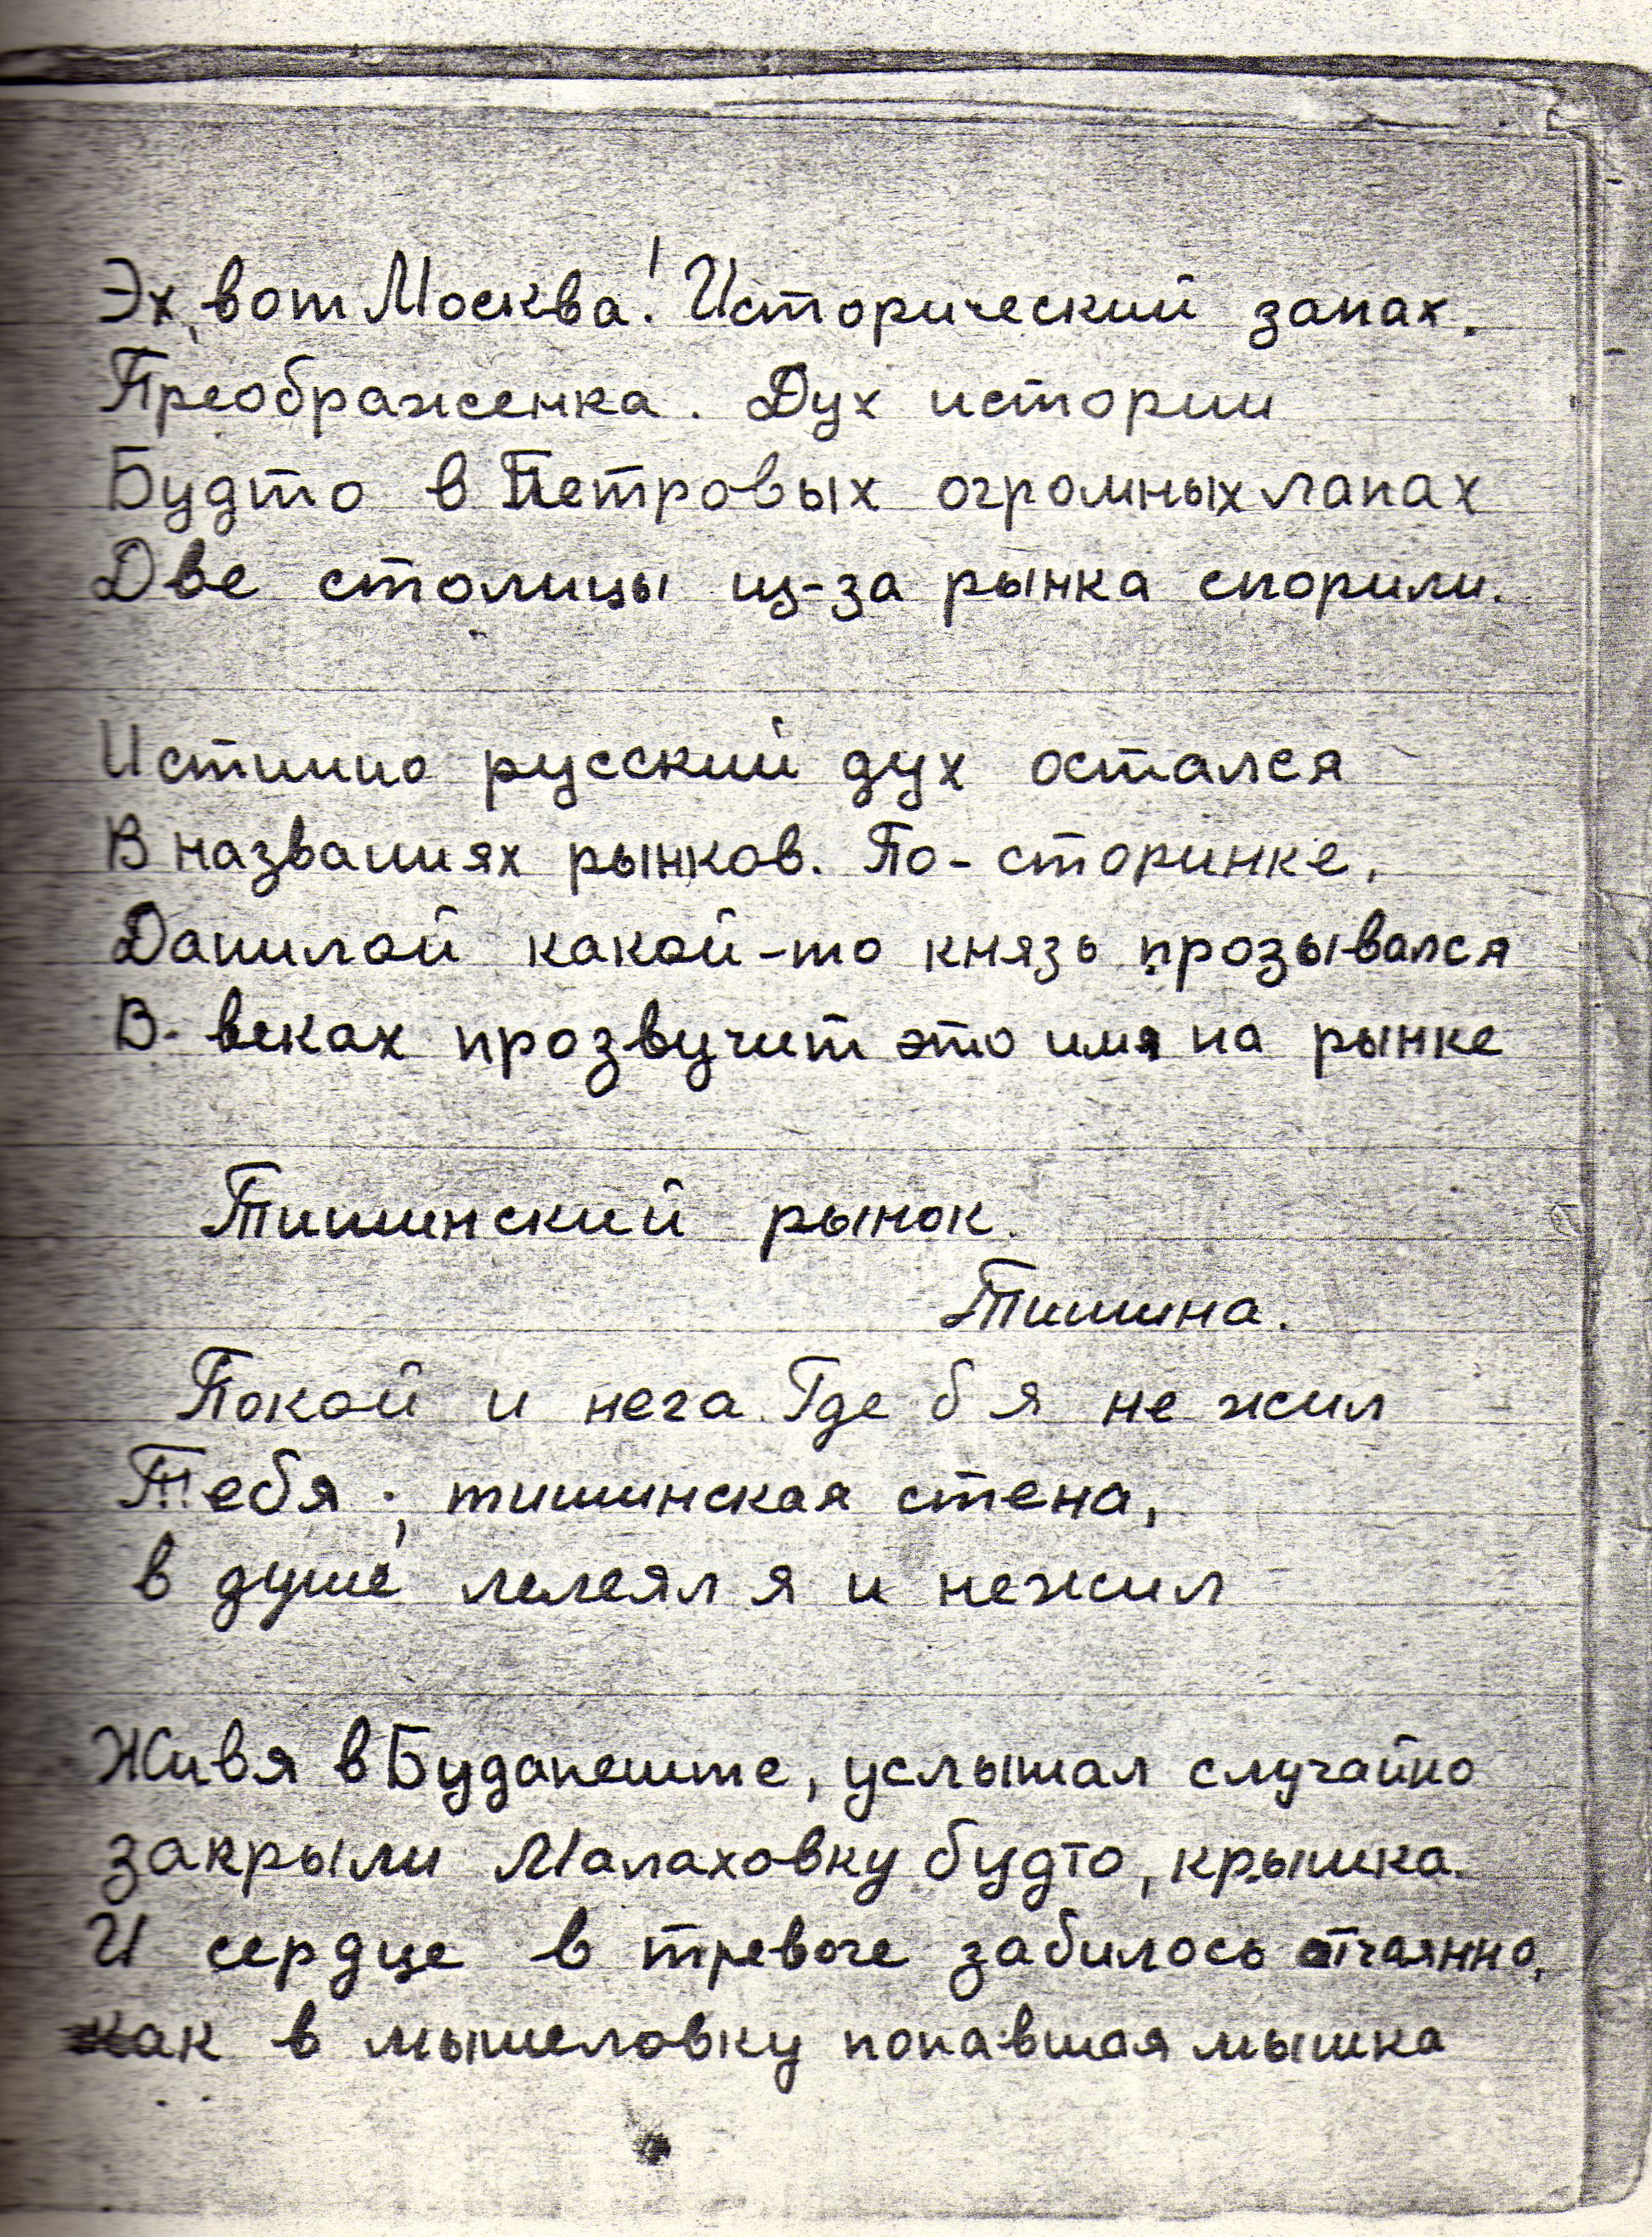
\includegraphics[width=\textwidth]{inc/Vynd/Vynd010}

\noindent
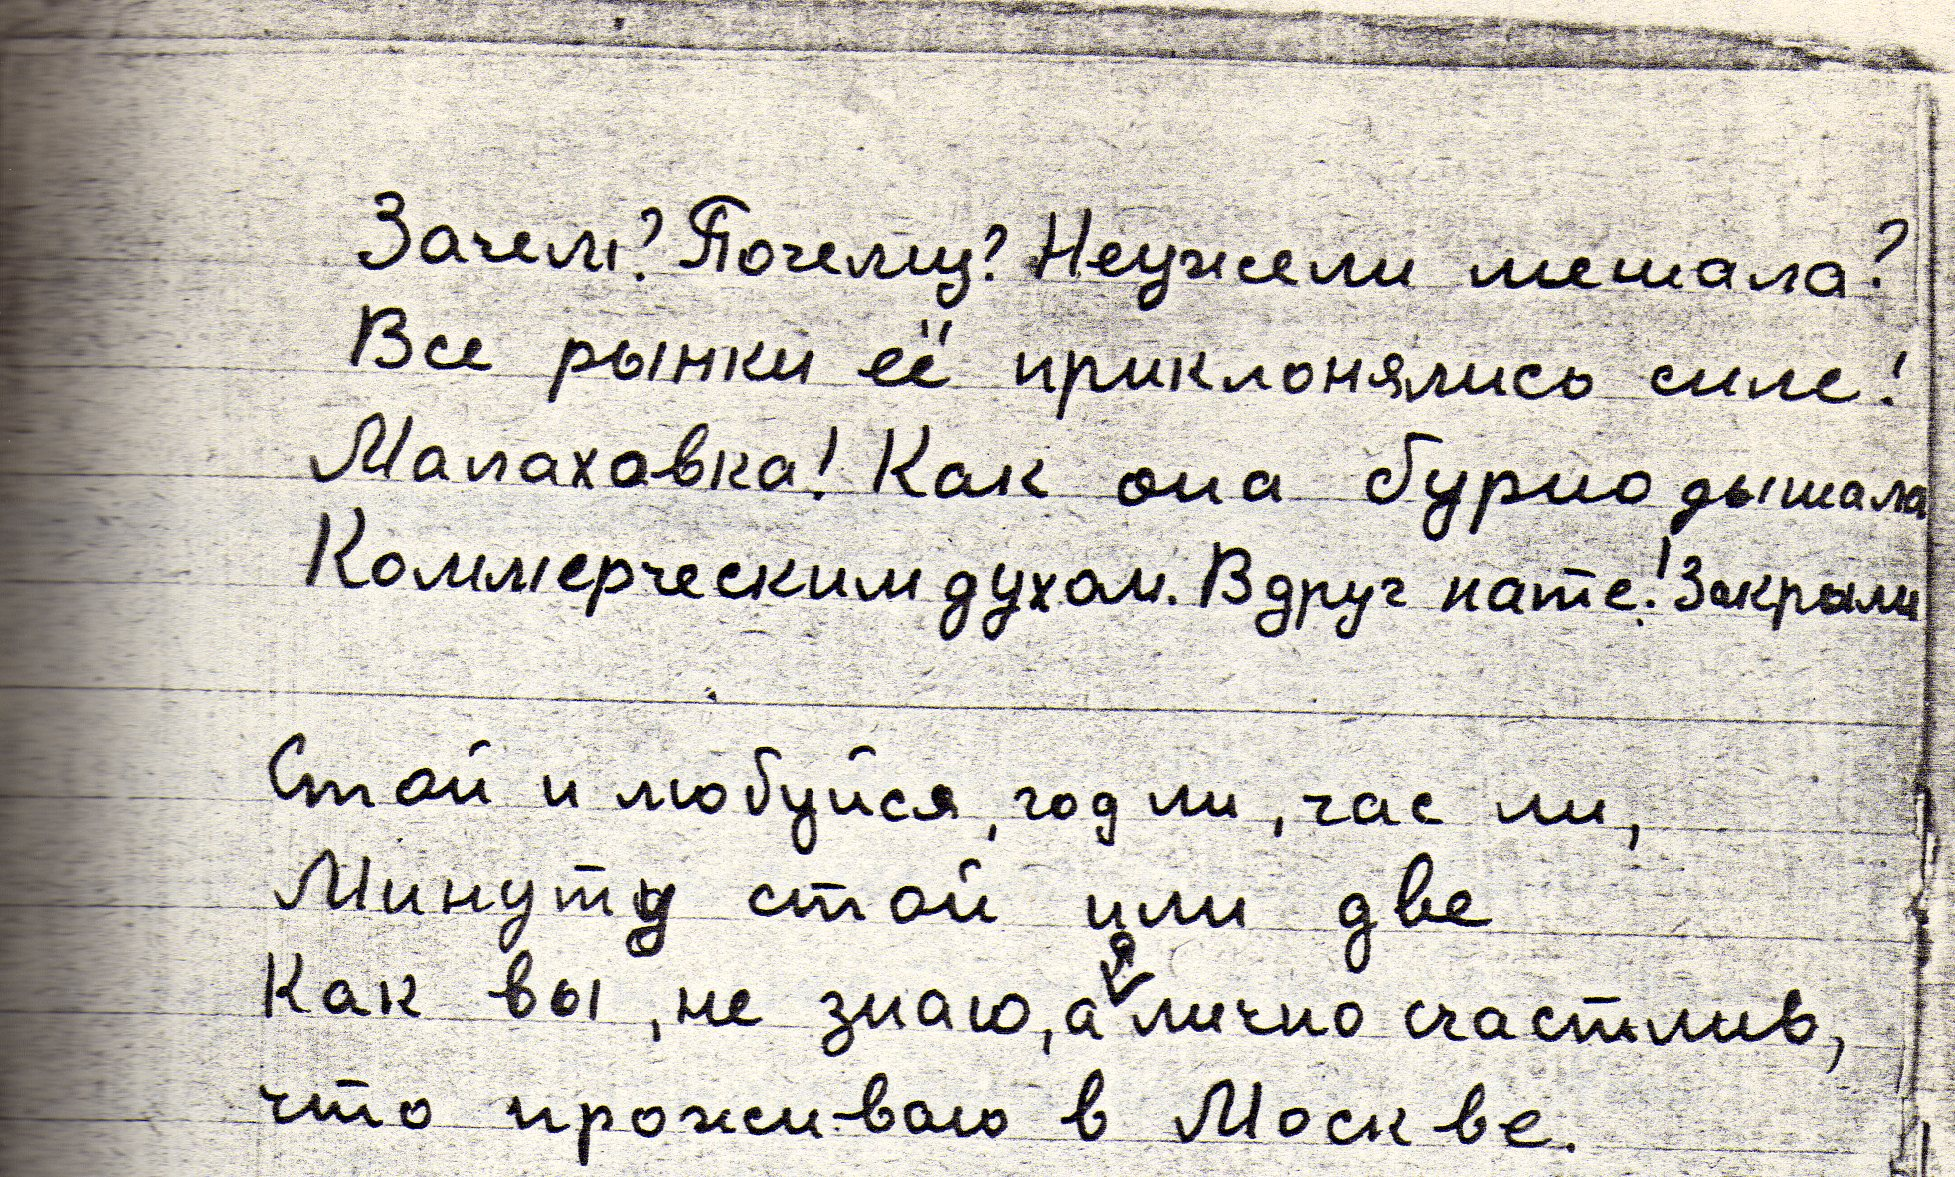
\includegraphics[width=\textwidth]{inc/Vynd/Vynd011}

\newpage


\noindent
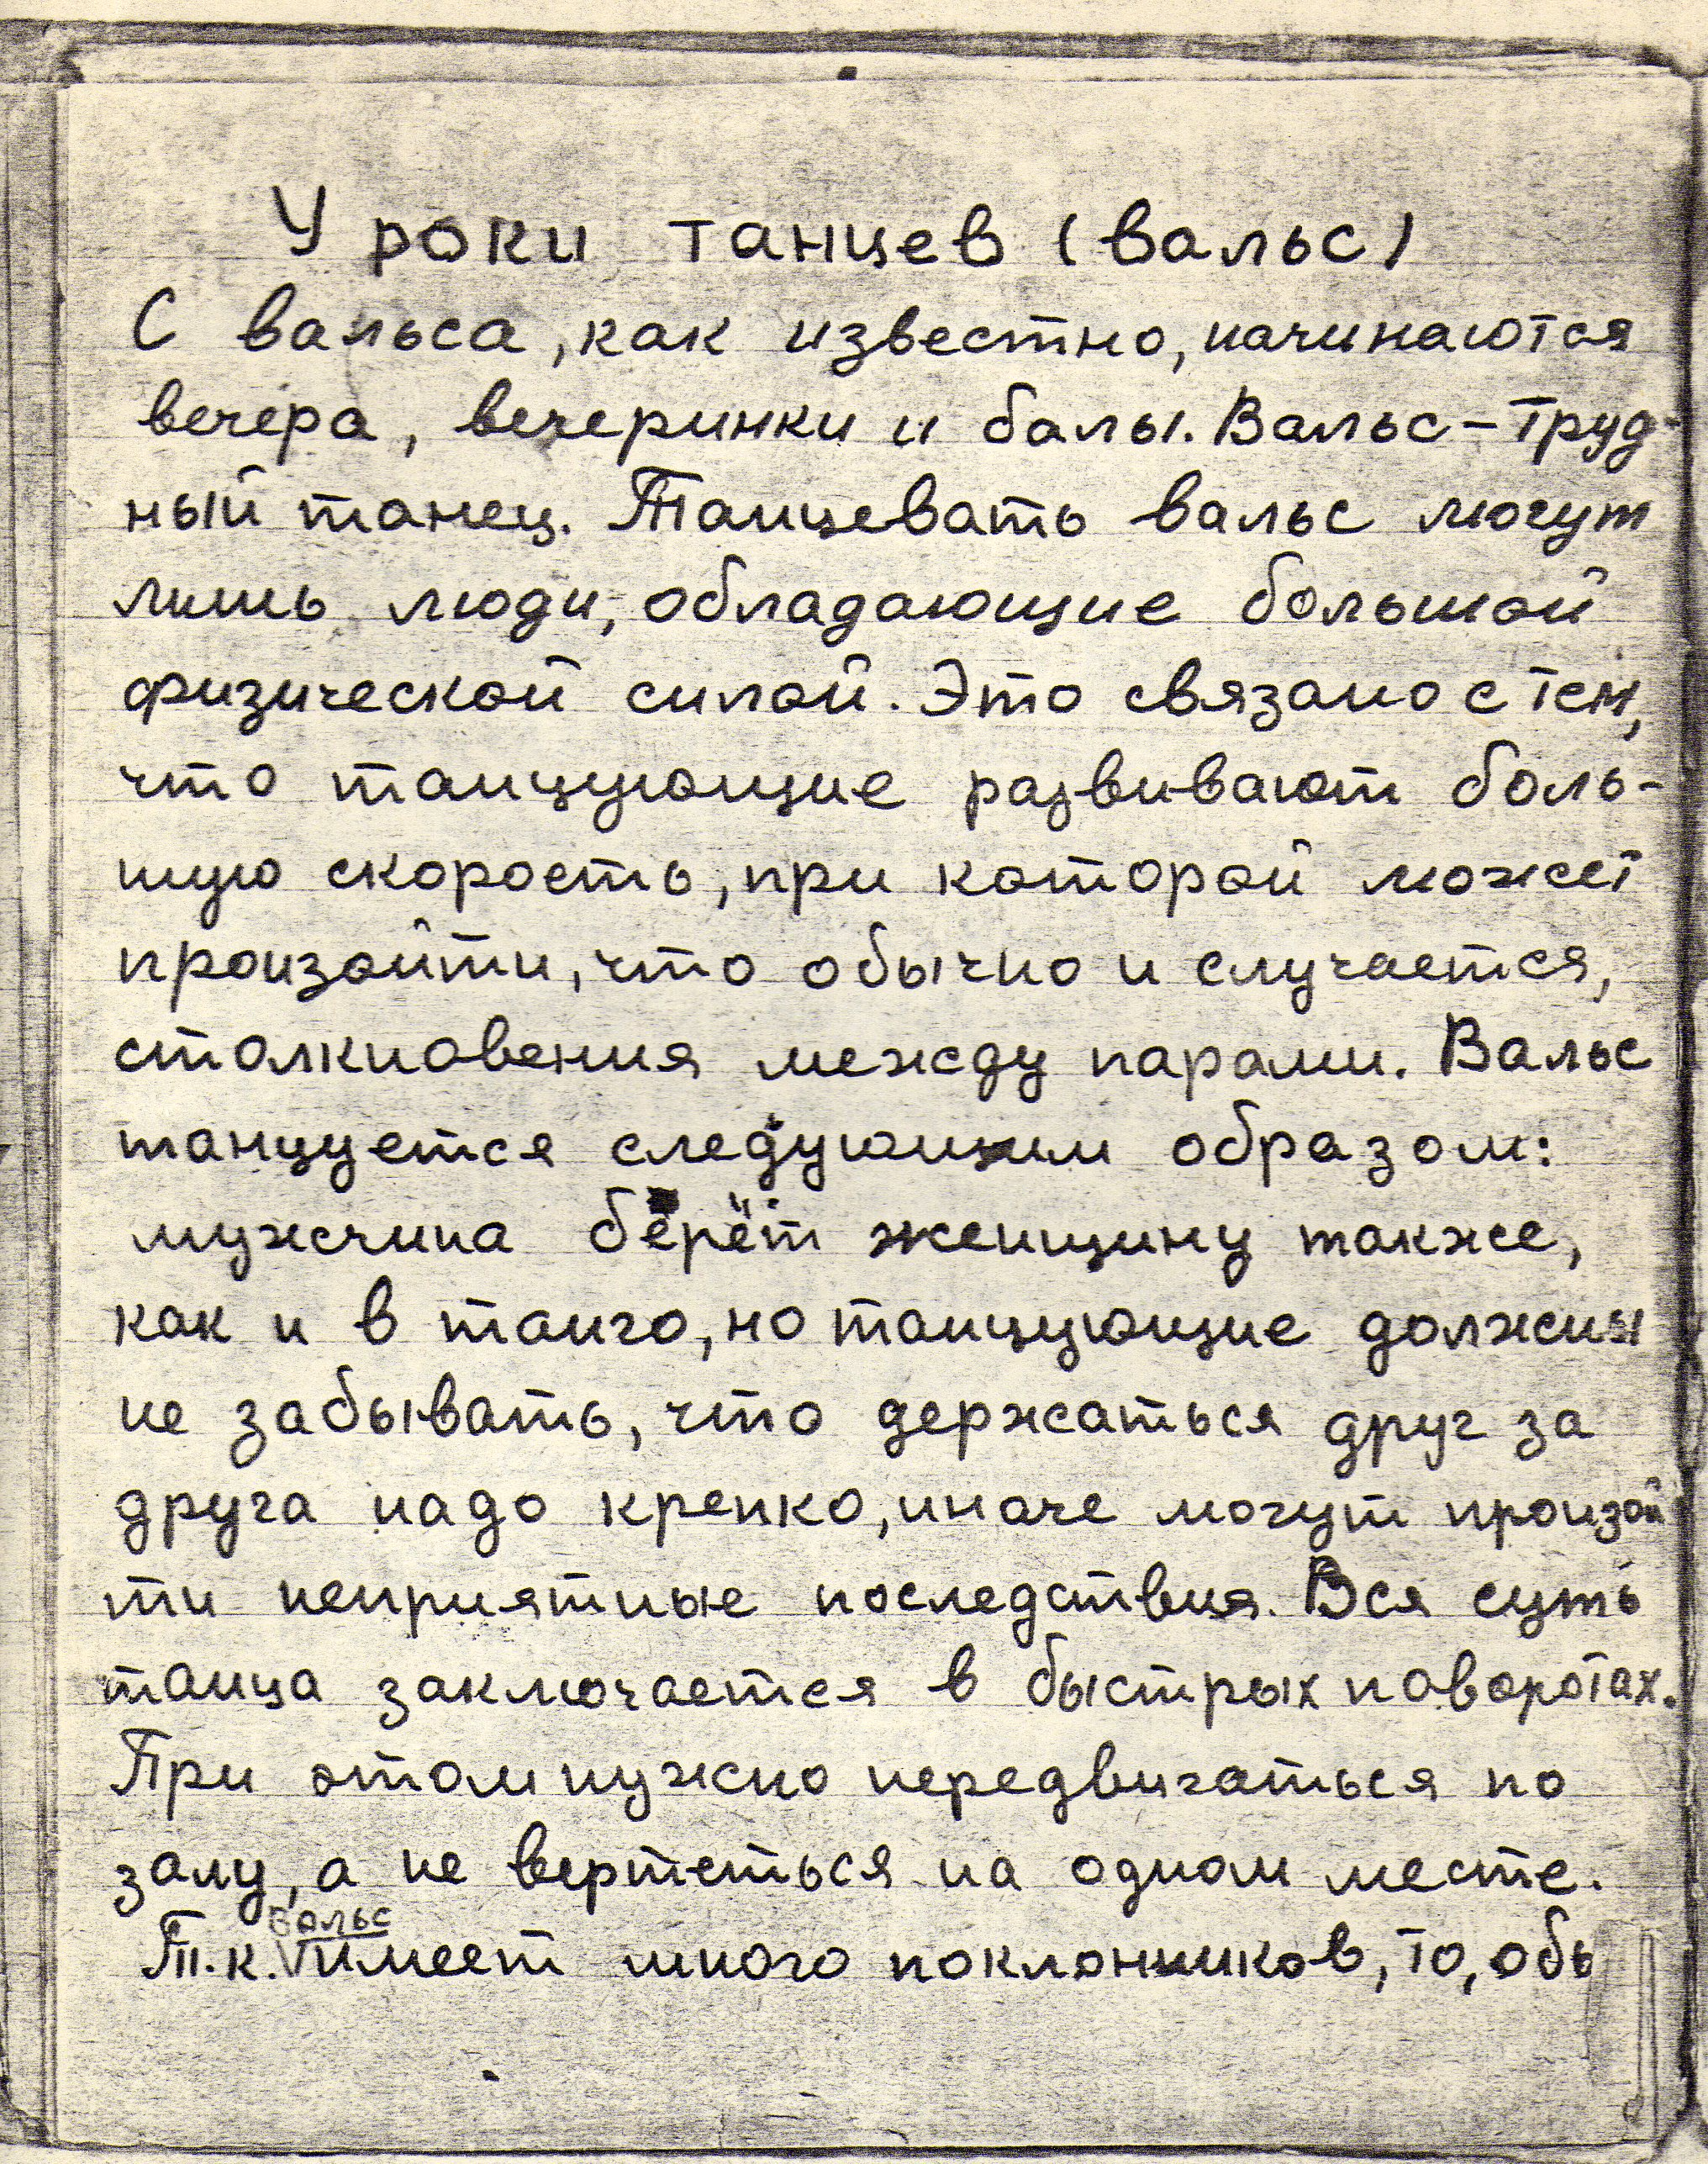
\includegraphics[width=\textwidth]{inc/Vynd/Vynd012}

\newpage

\noindent
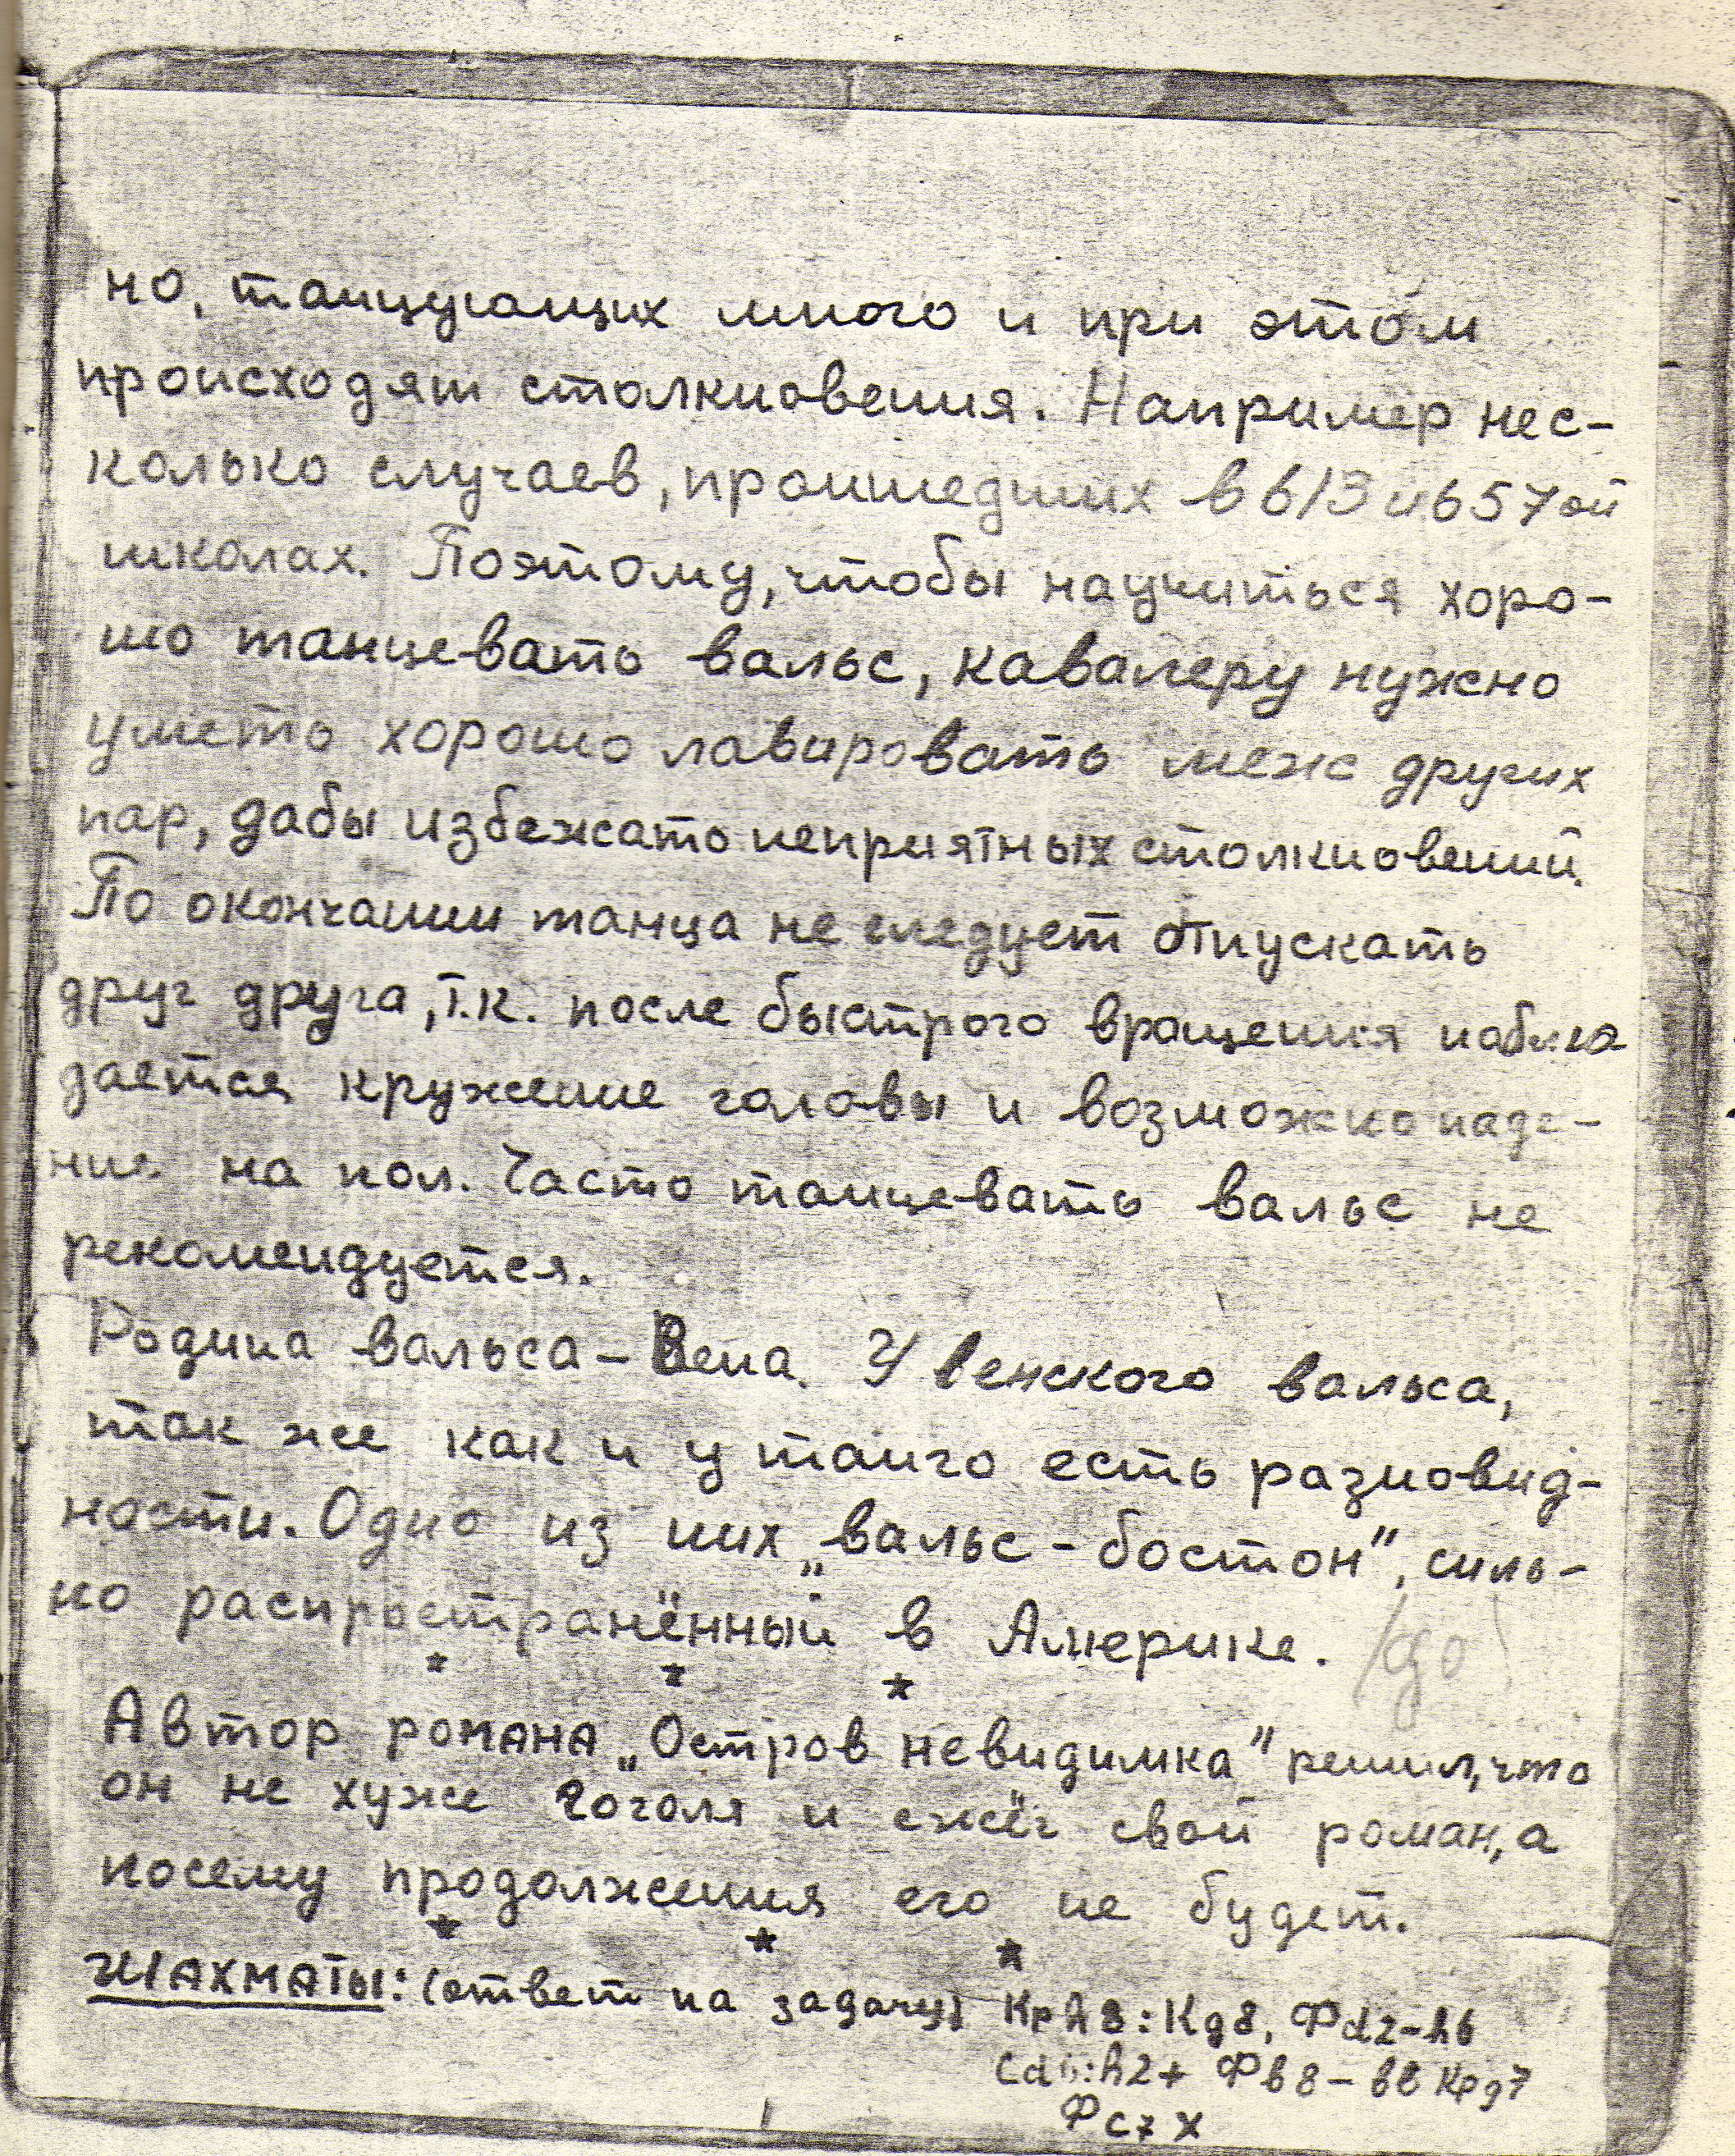
\includegraphics[width=\textwidth]{inc/Vynd/Vynd013}

\section*{Из <<Вундеркинда>> юбилейного. 1987 год.}

\noindent
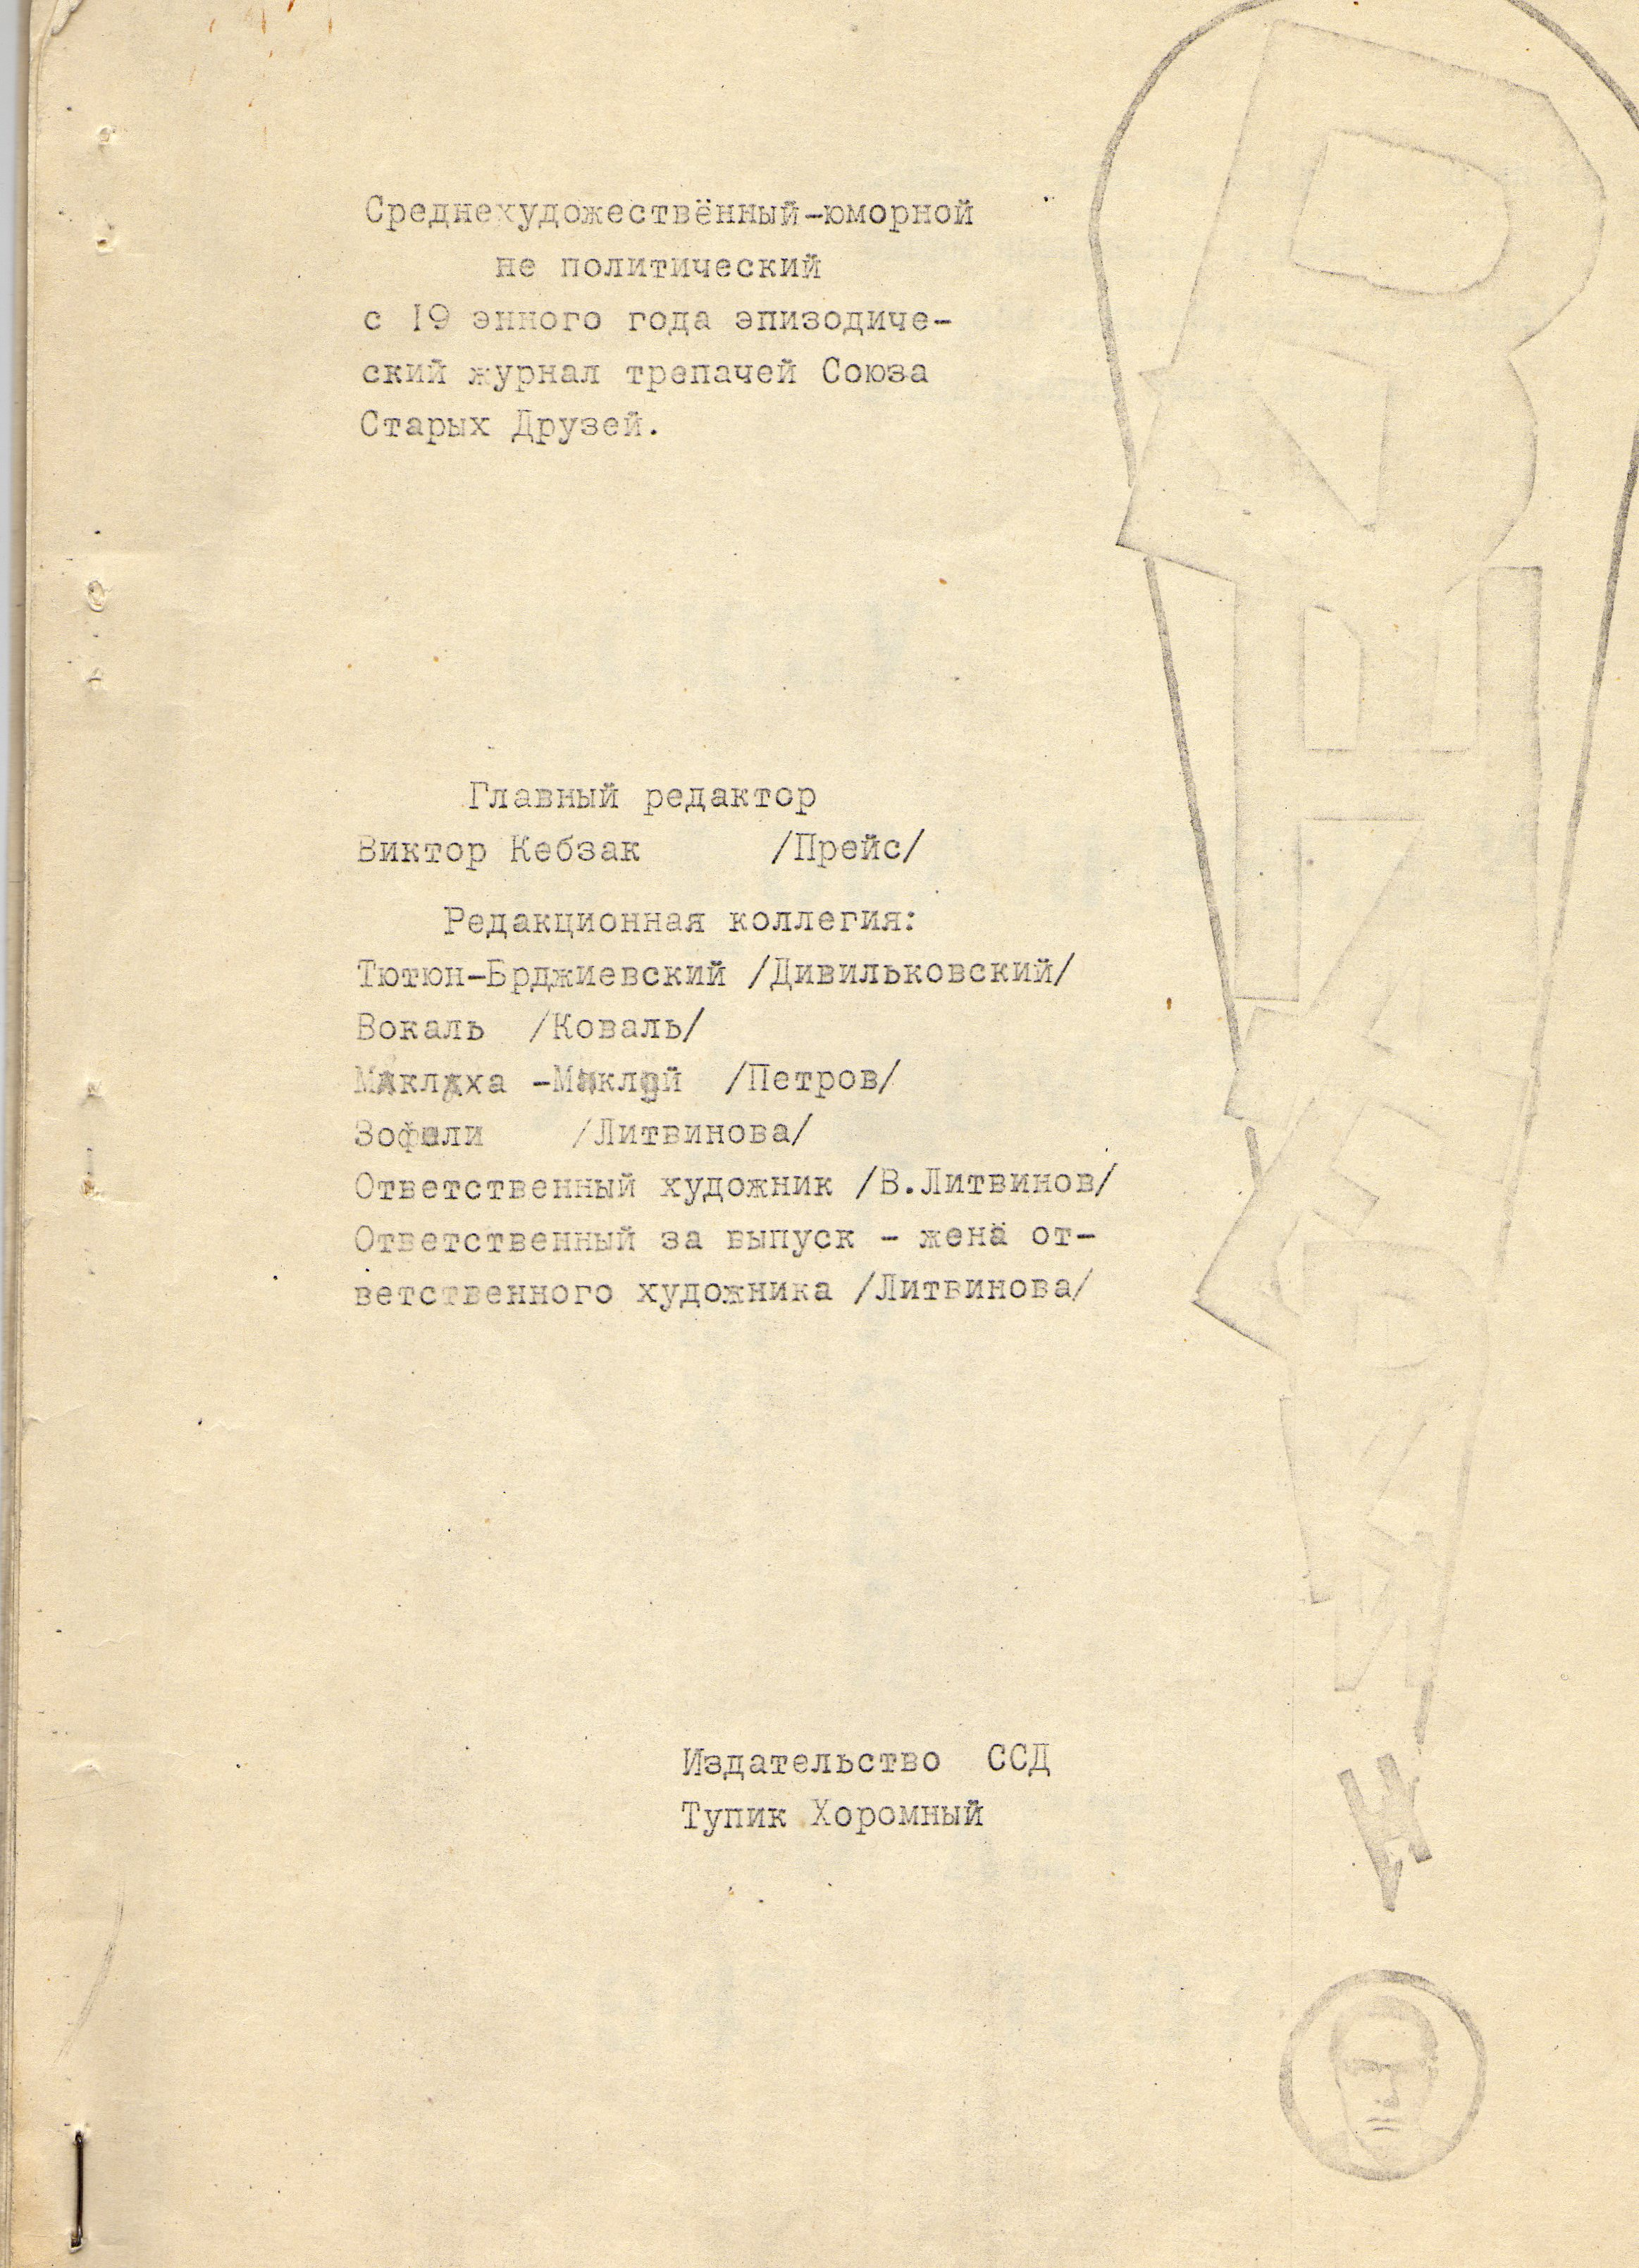
\includegraphics[width=\textwidth]{inc/Vynd/Vynd014}

\noindent
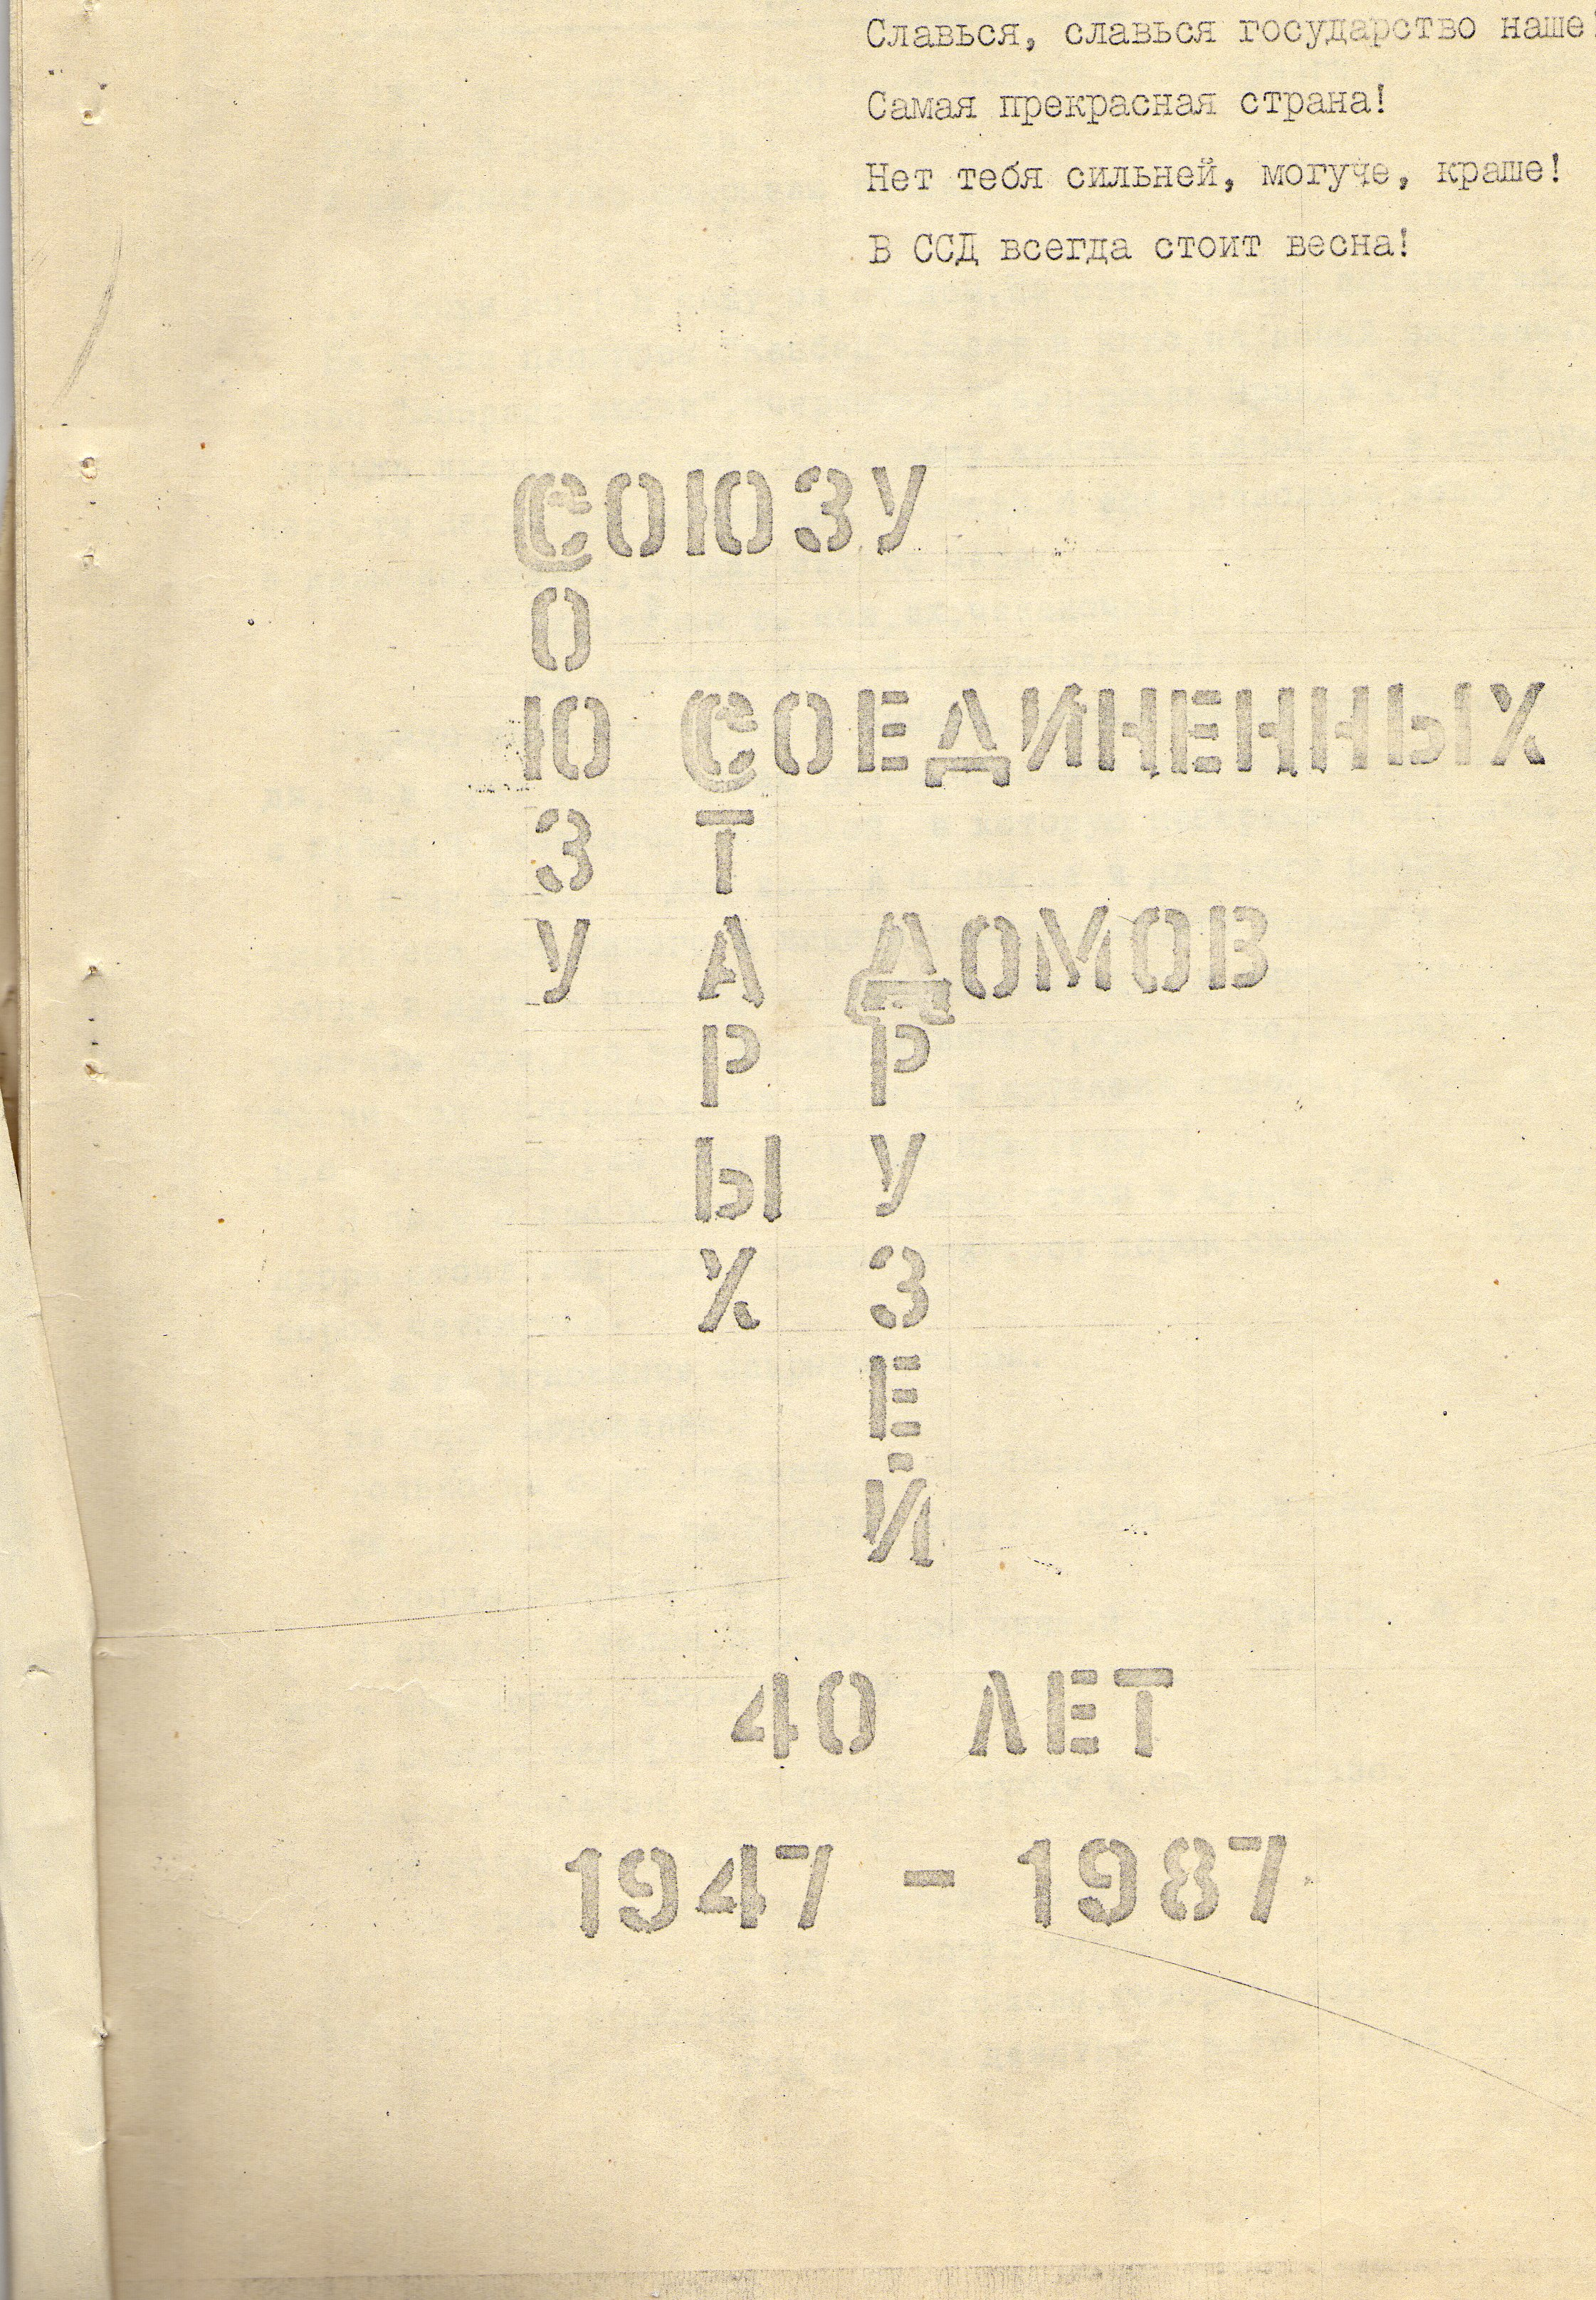
\includegraphics[width=\textwidth]{inc/Vynd/Vynd016}

\noindent
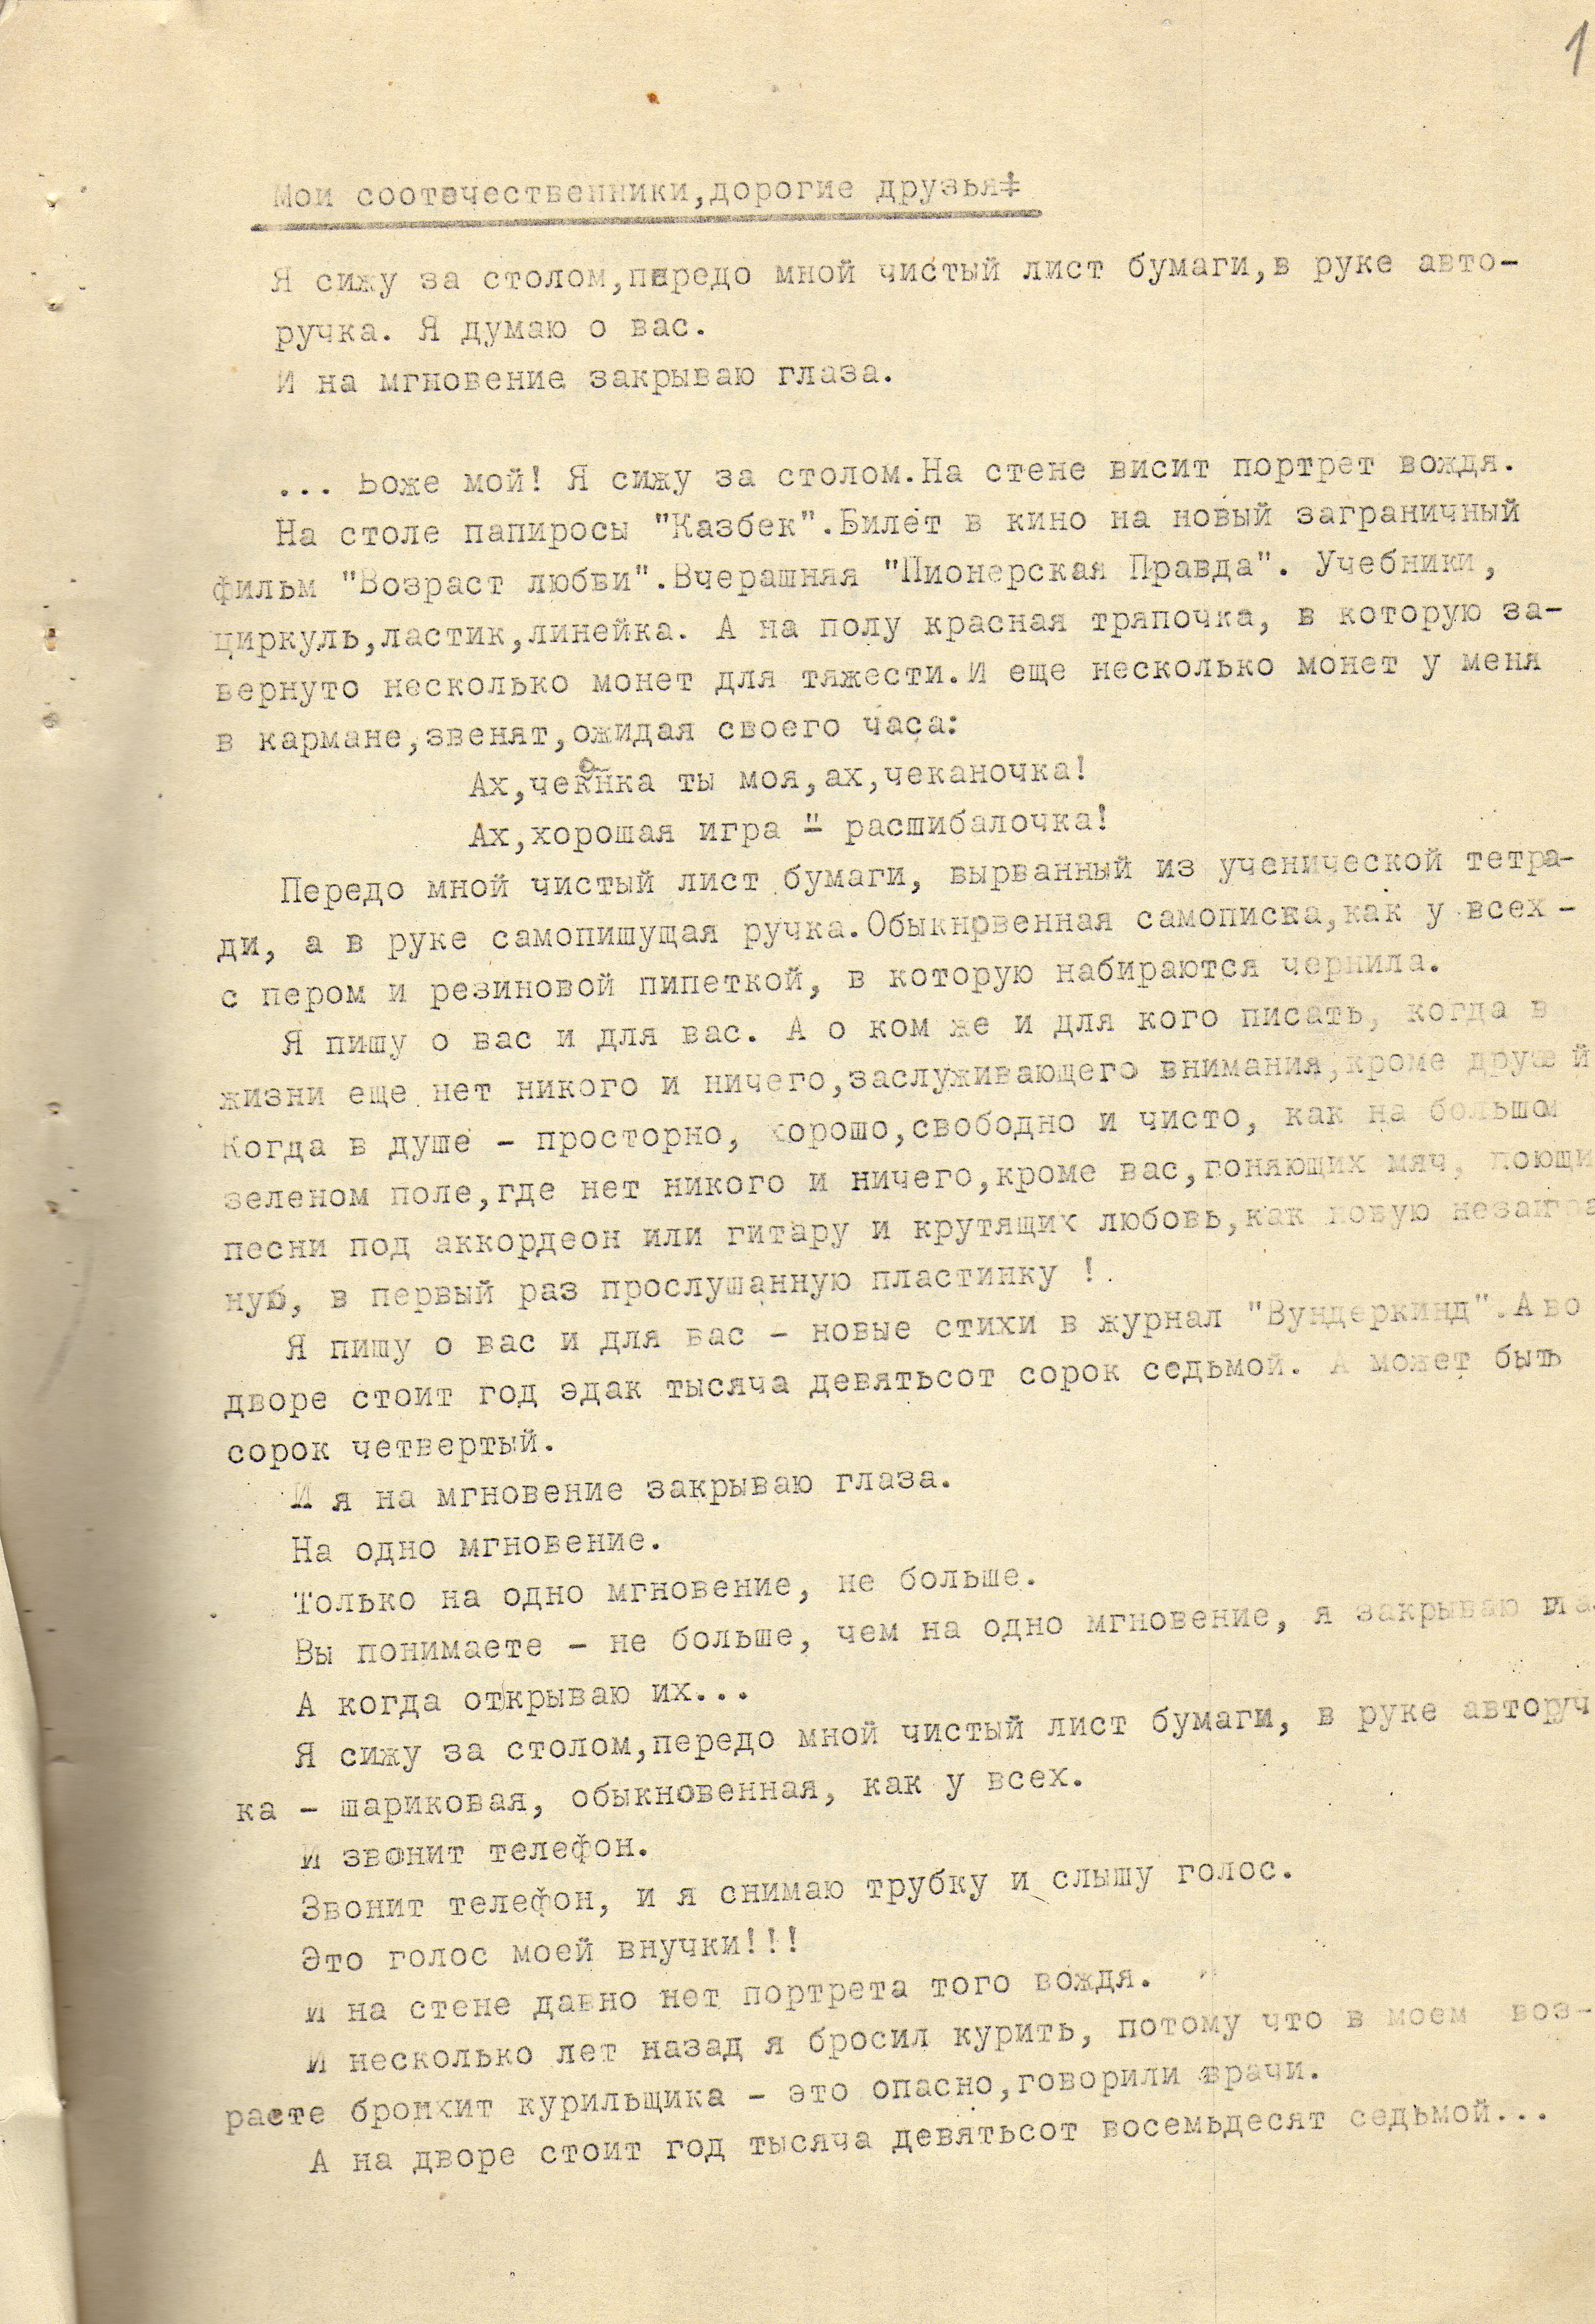
\includegraphics[width=\textwidth]{inc/Vynd/Vynd017}

\noindent
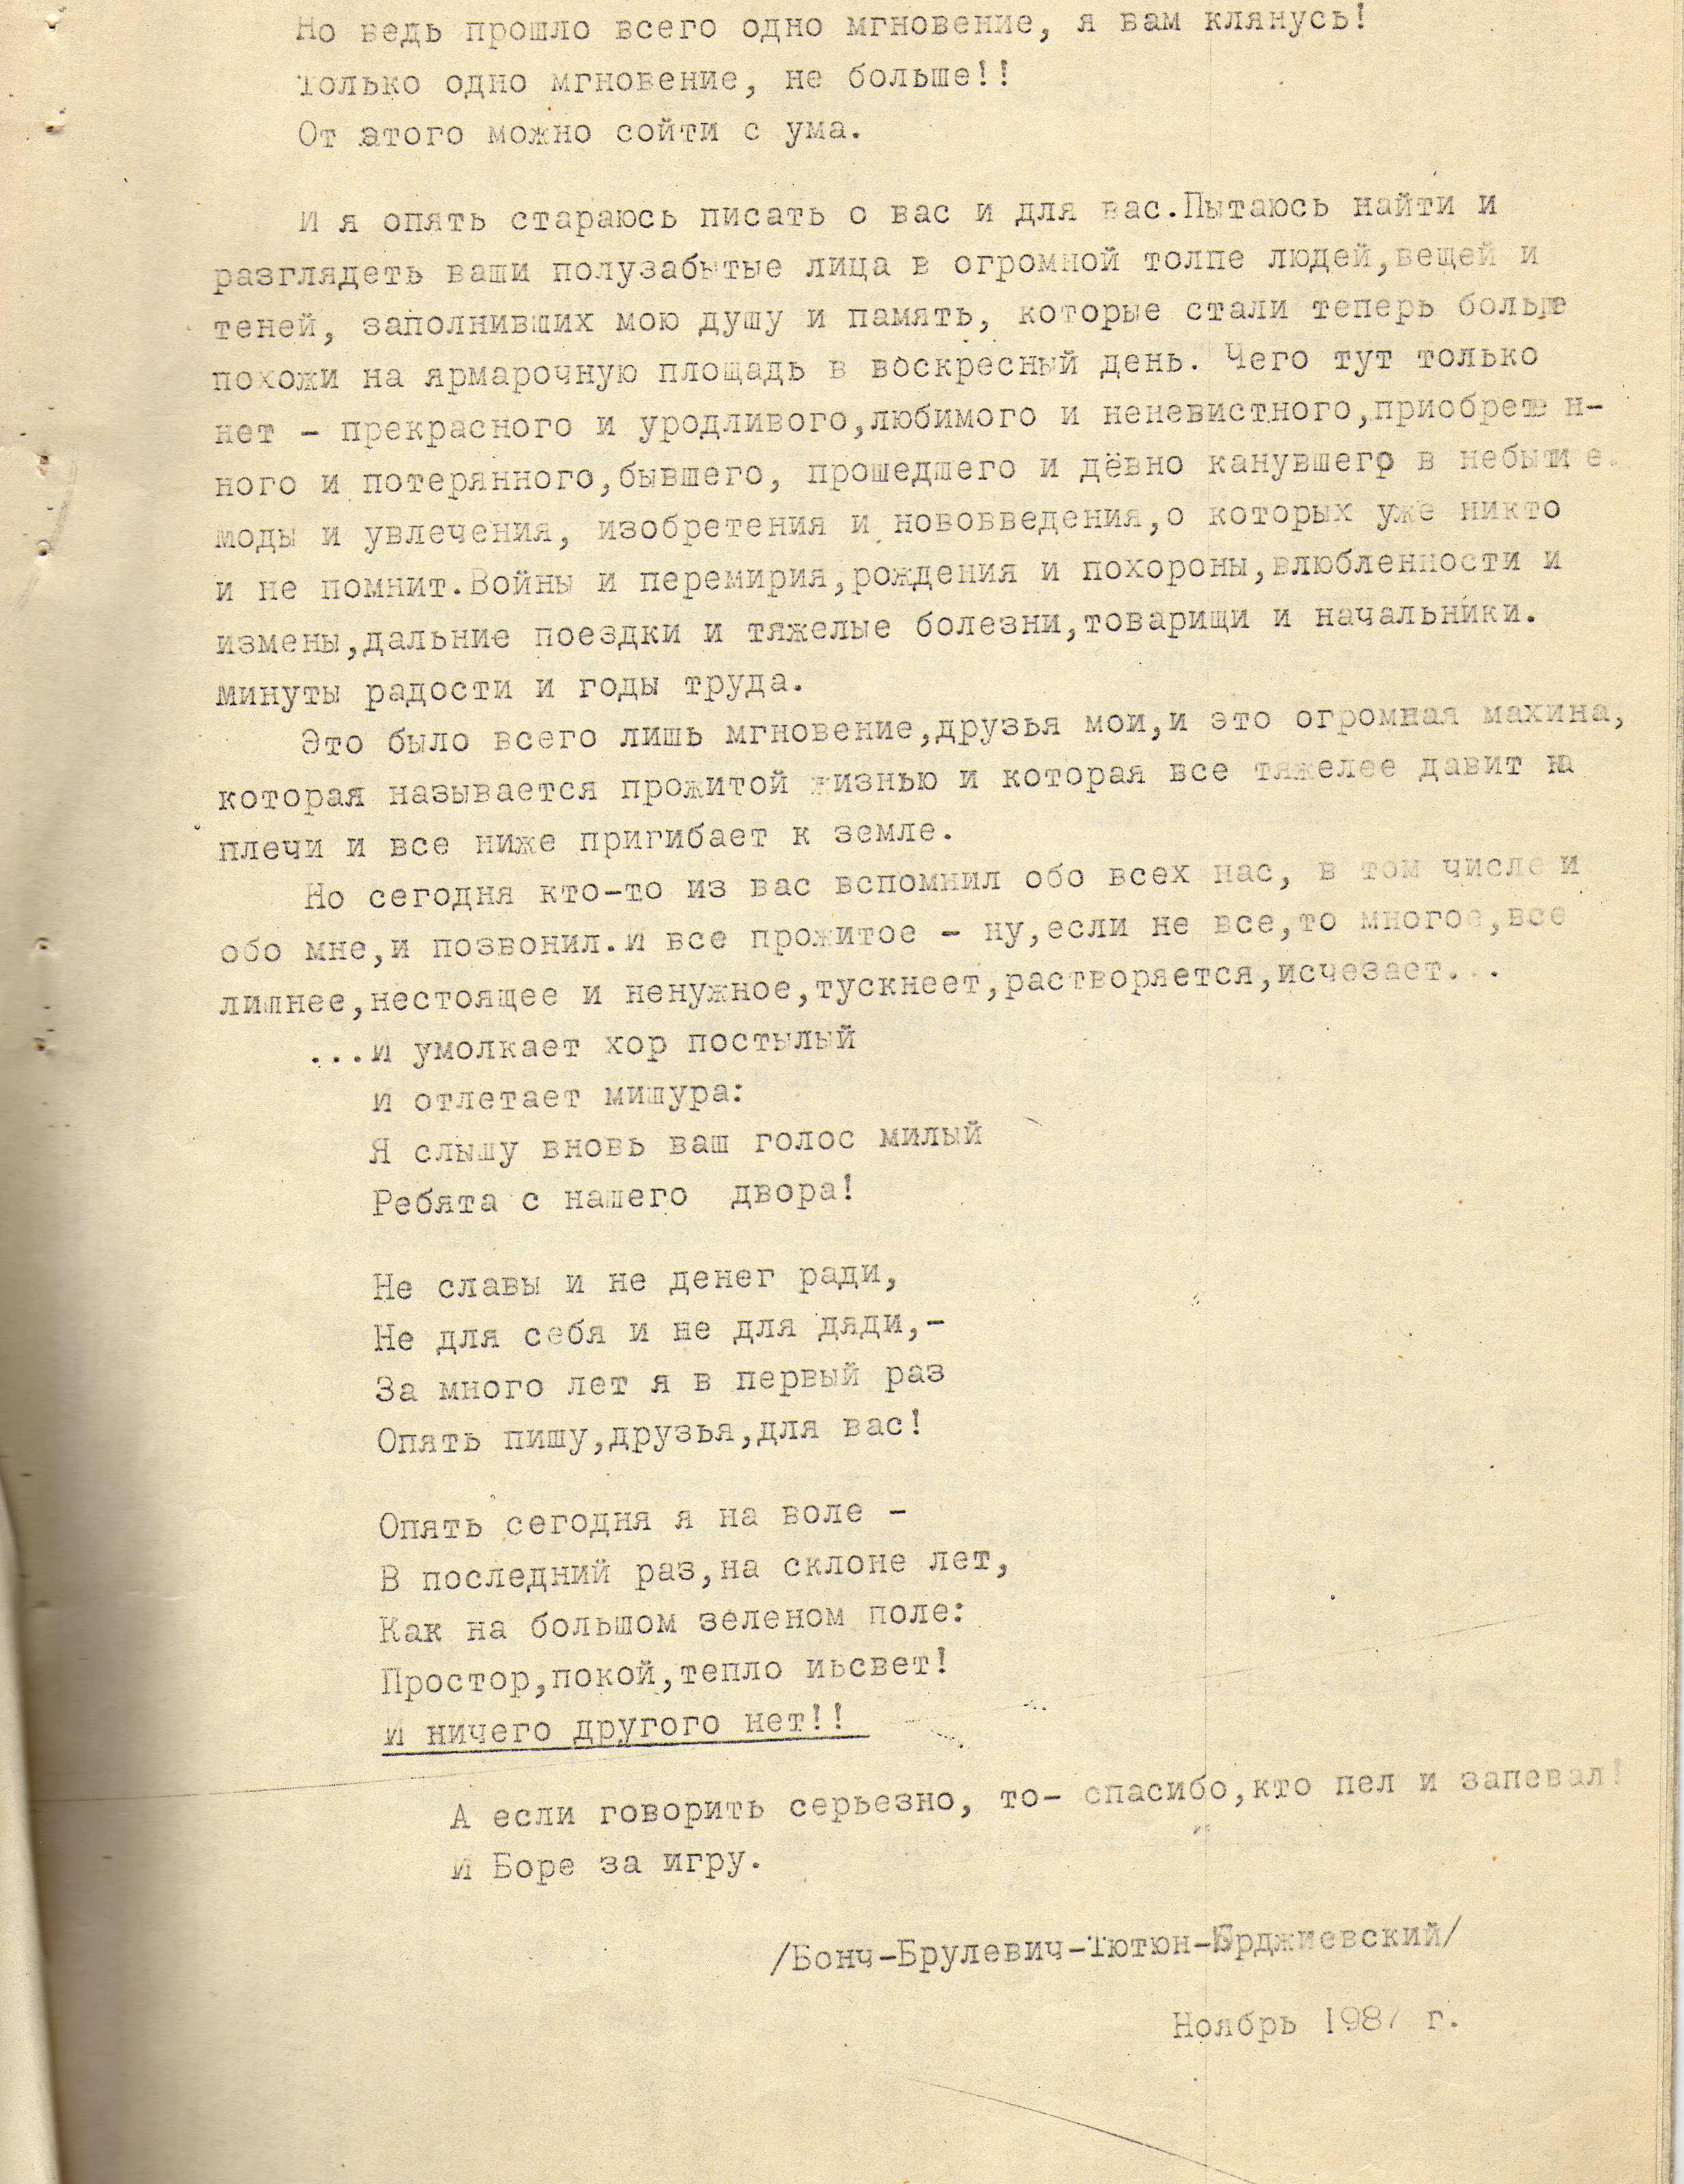
\includegraphics[width=\textwidth]{inc/Vynd/Vynd018}

\noindent
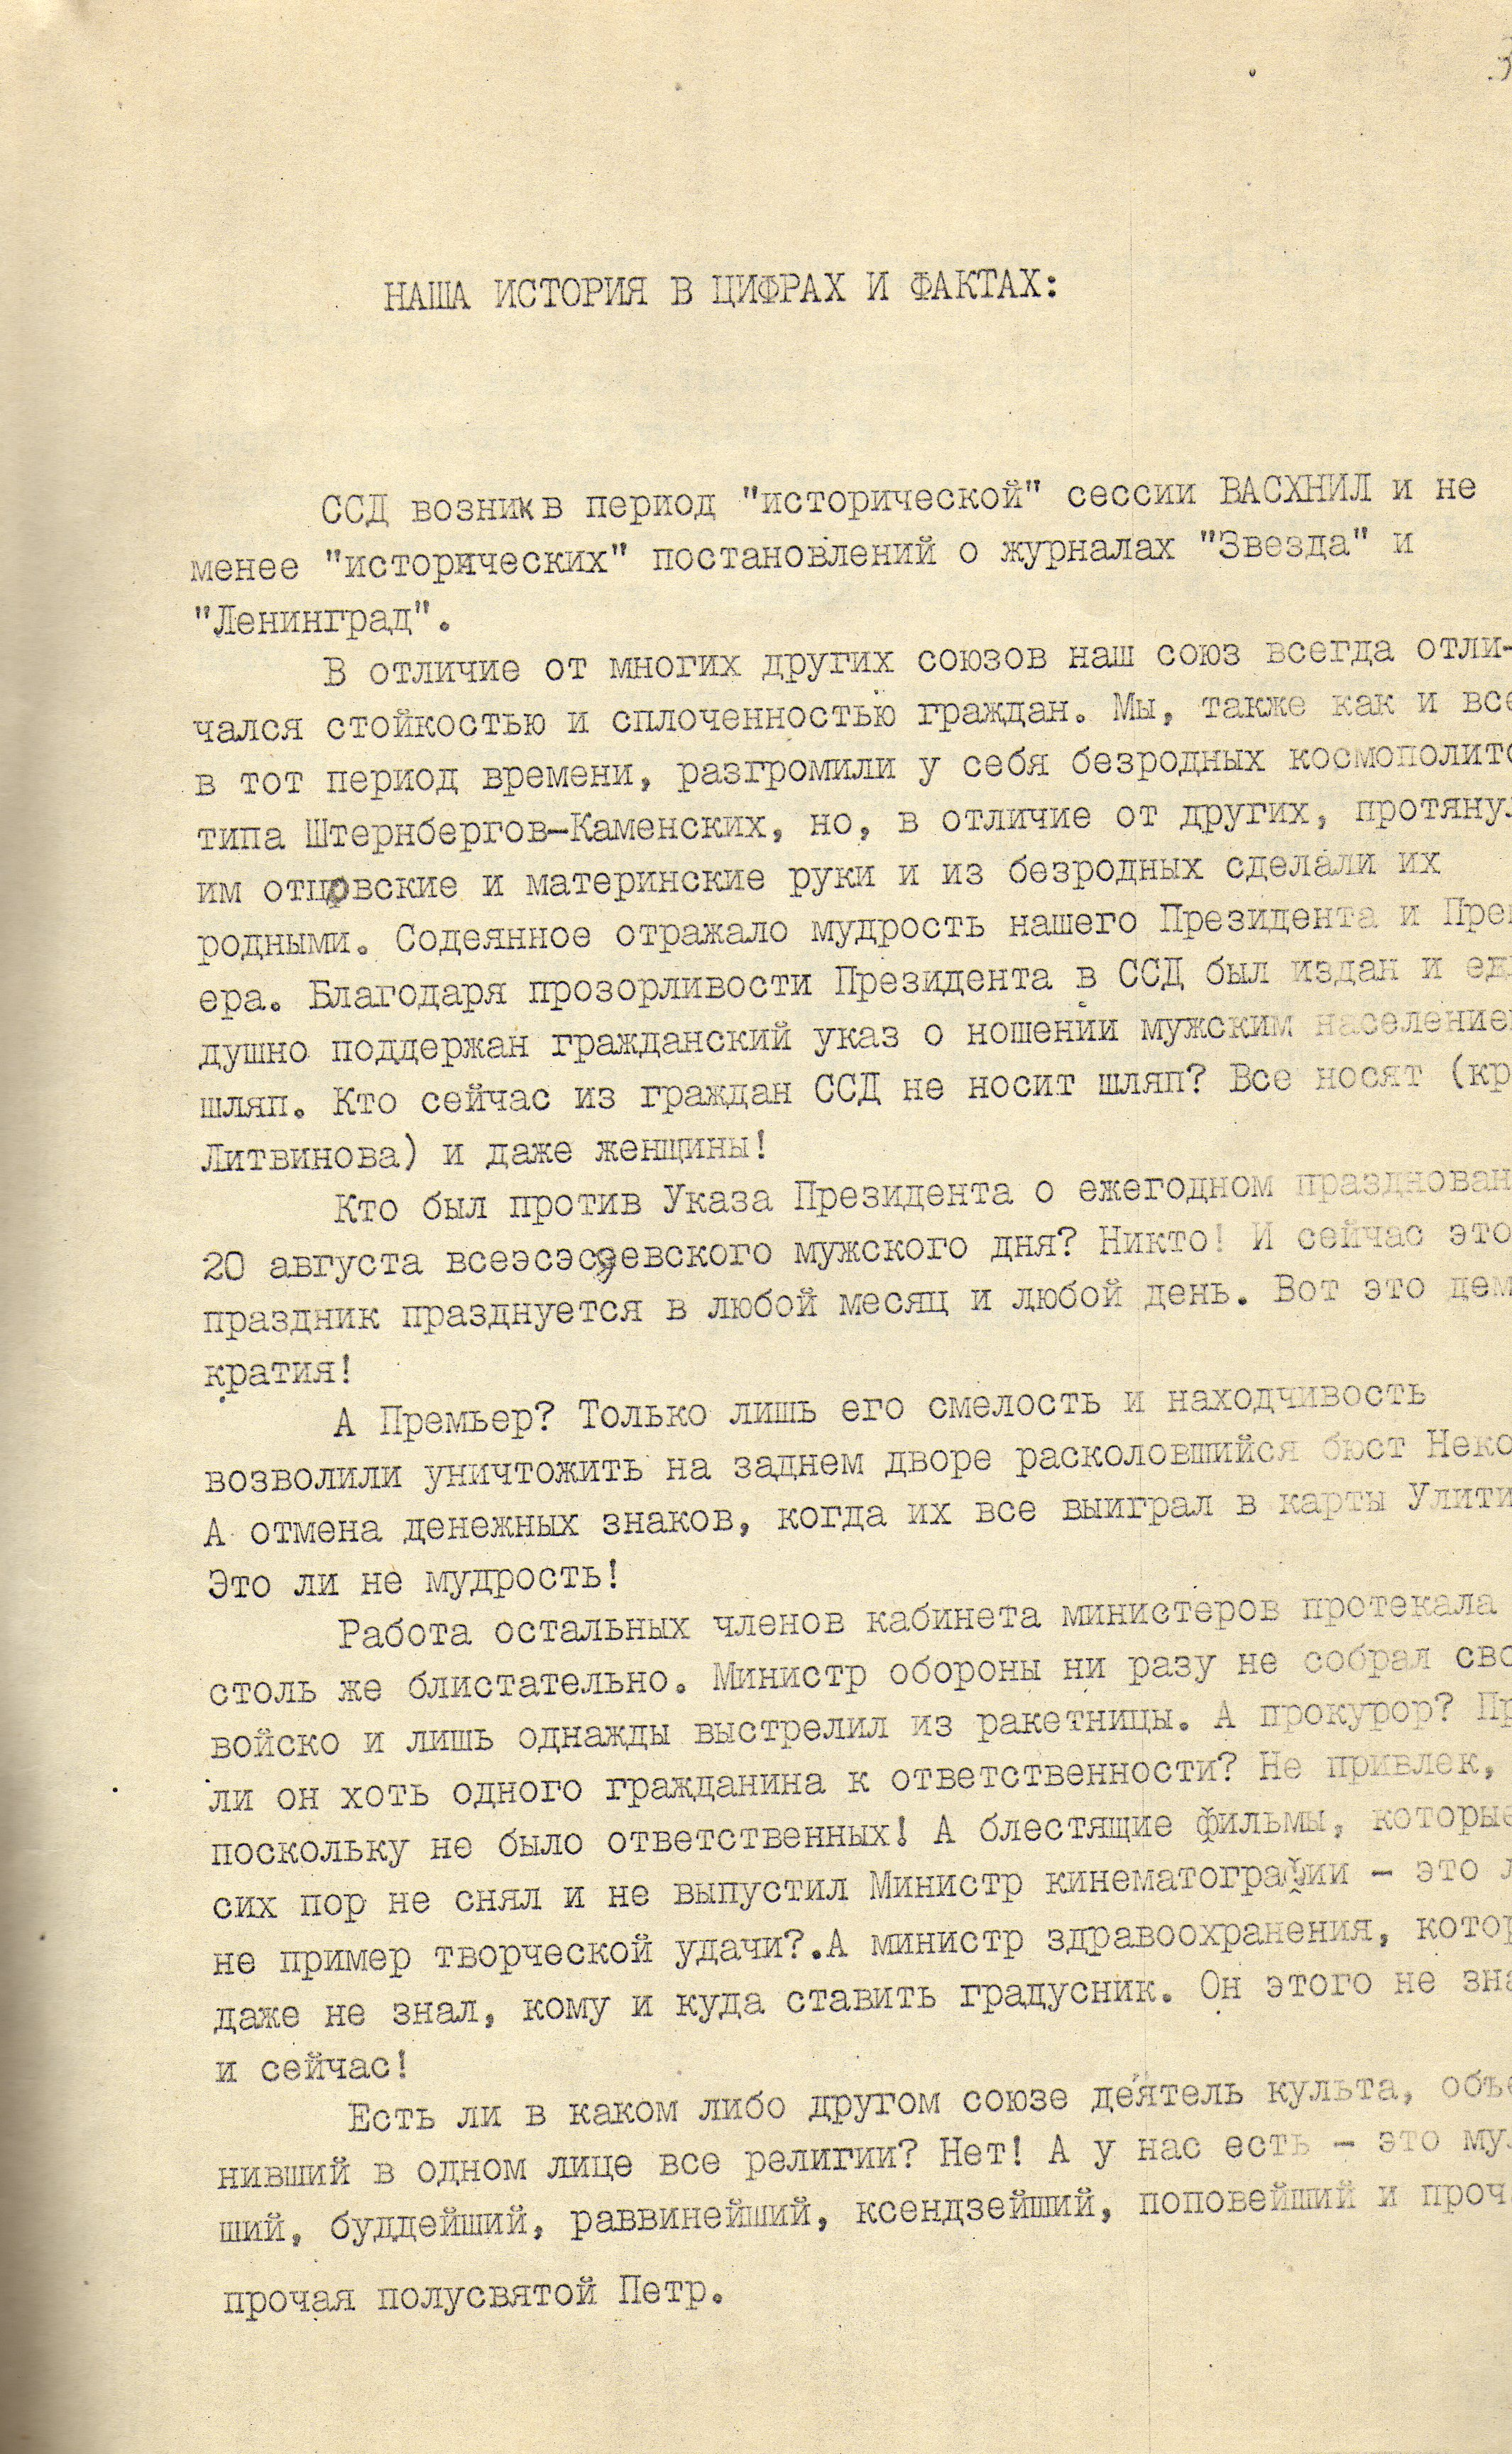
\includegraphics[width=\textwidth]{inc/Vynd/Vynd019}

\noindent
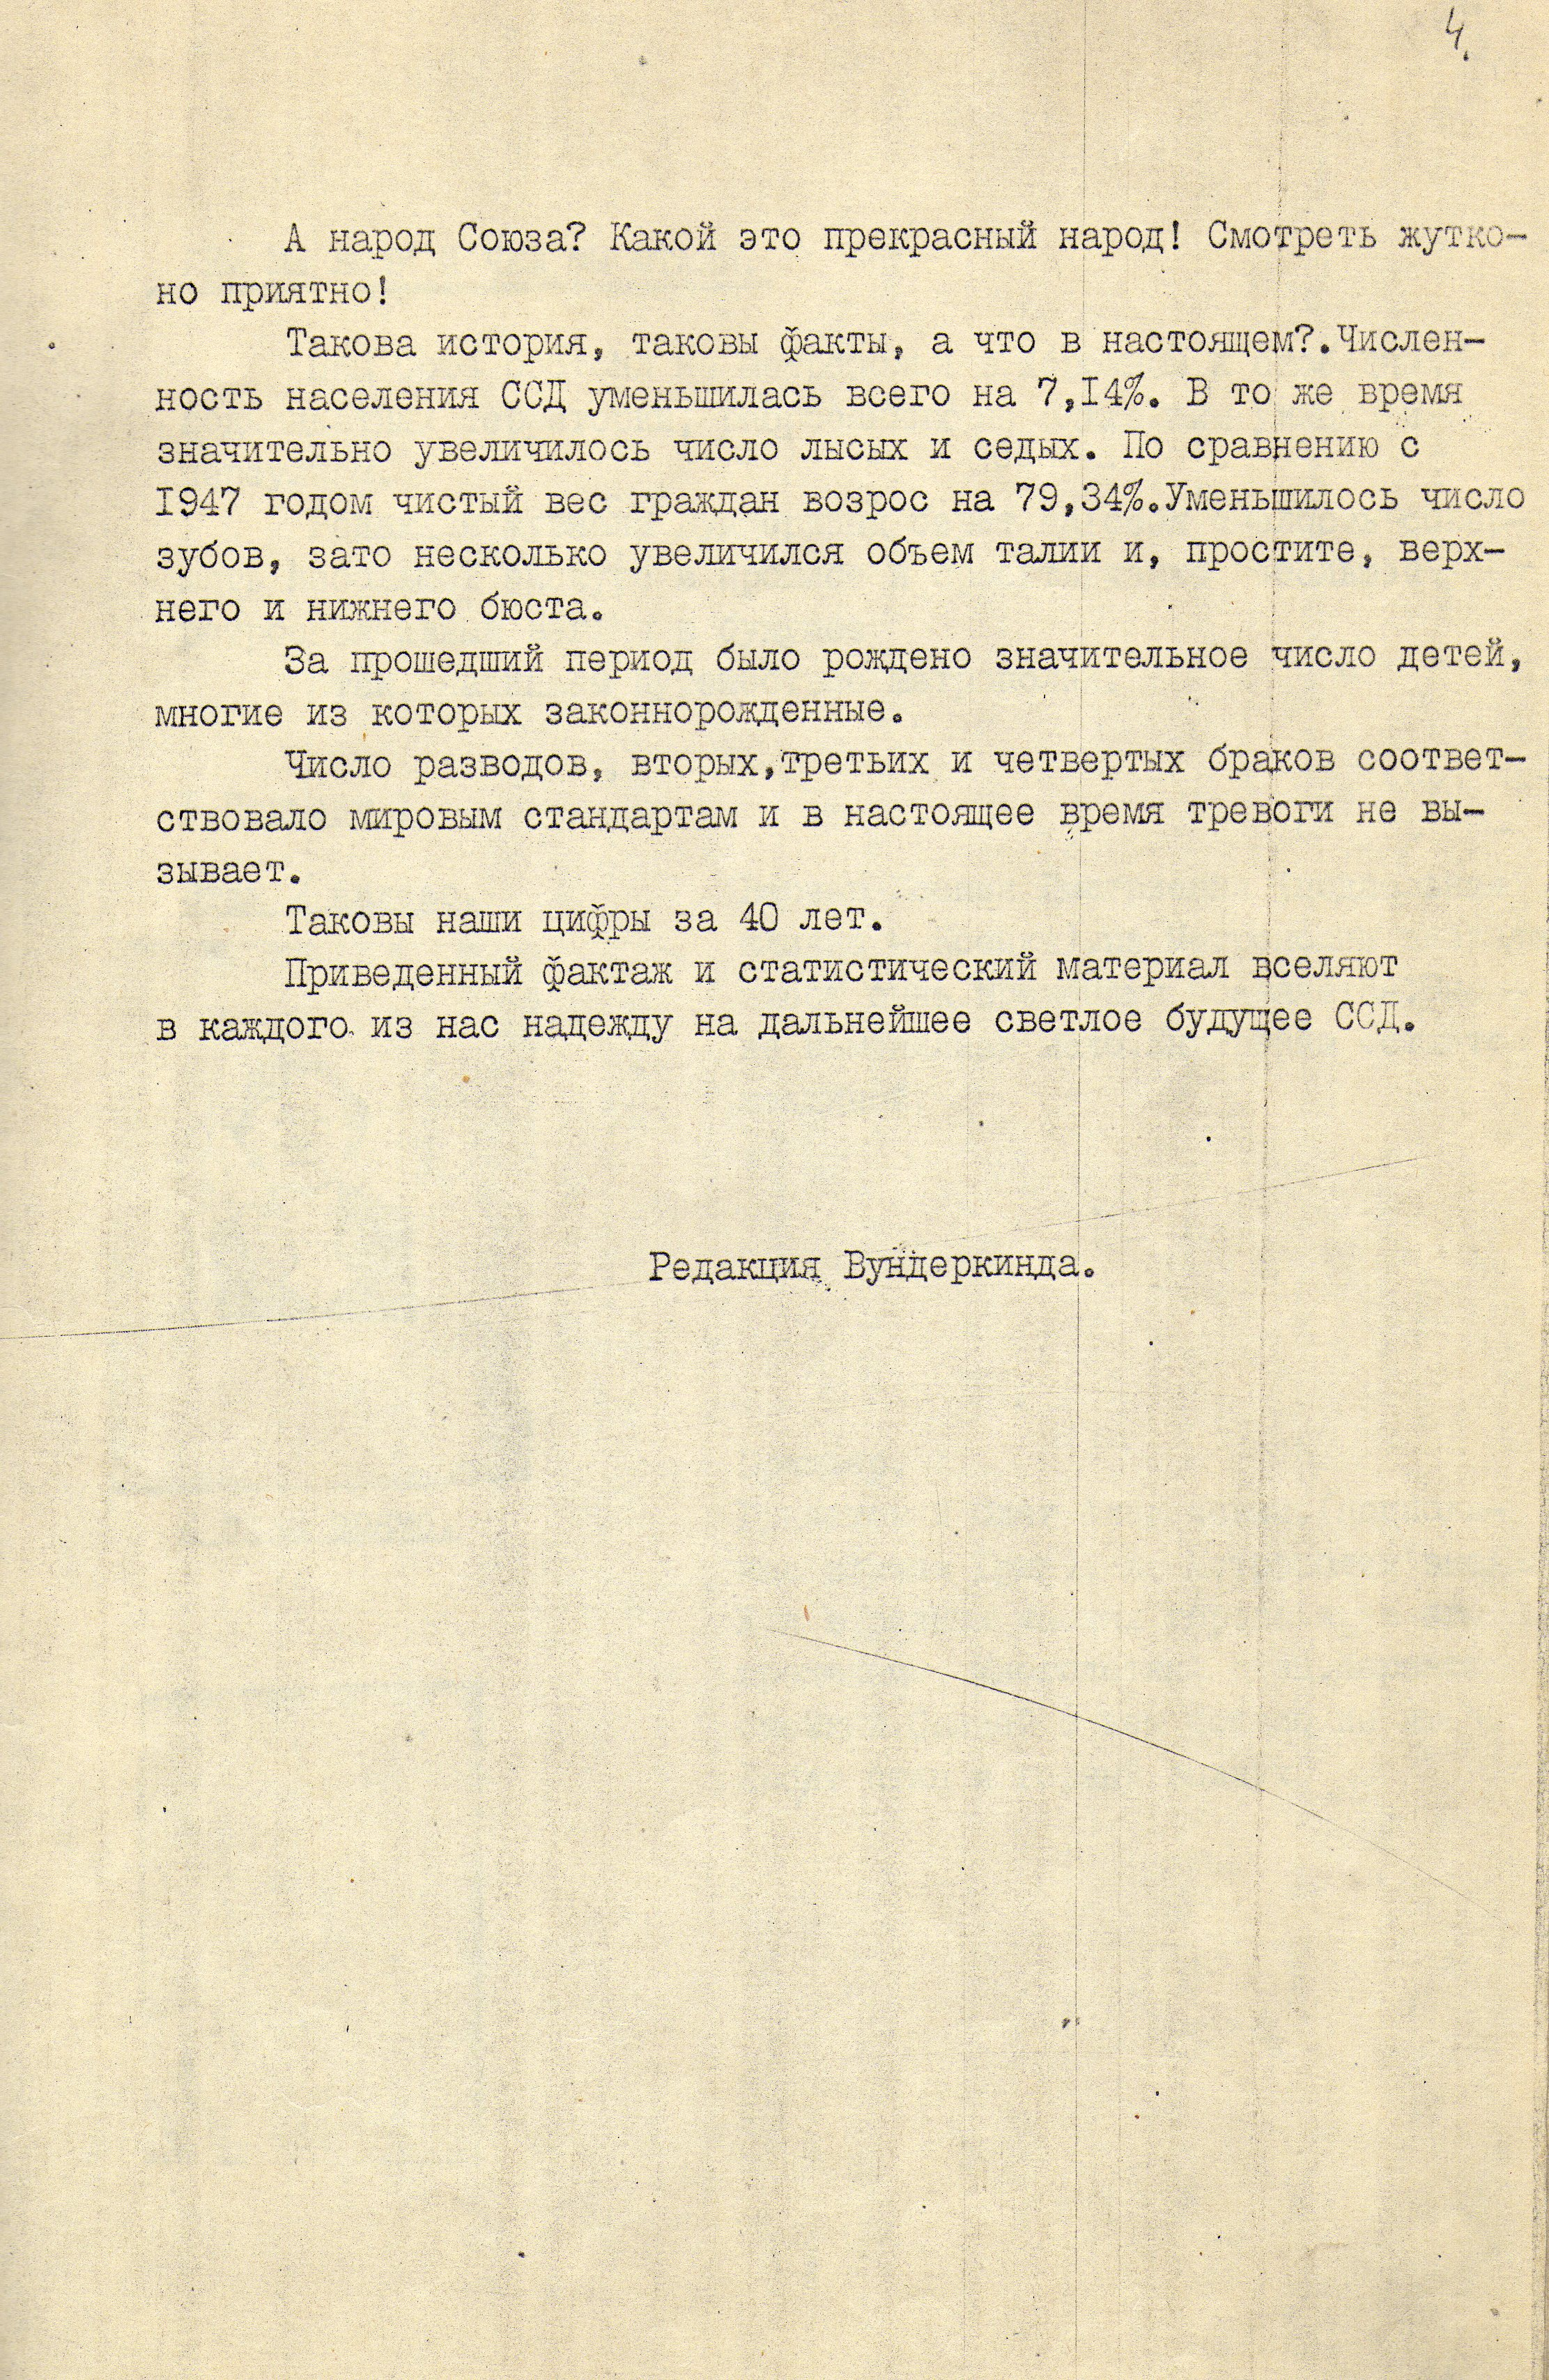
\includegraphics[width=\textwidth]{inc/Vynd/Vynd020}

\noindent
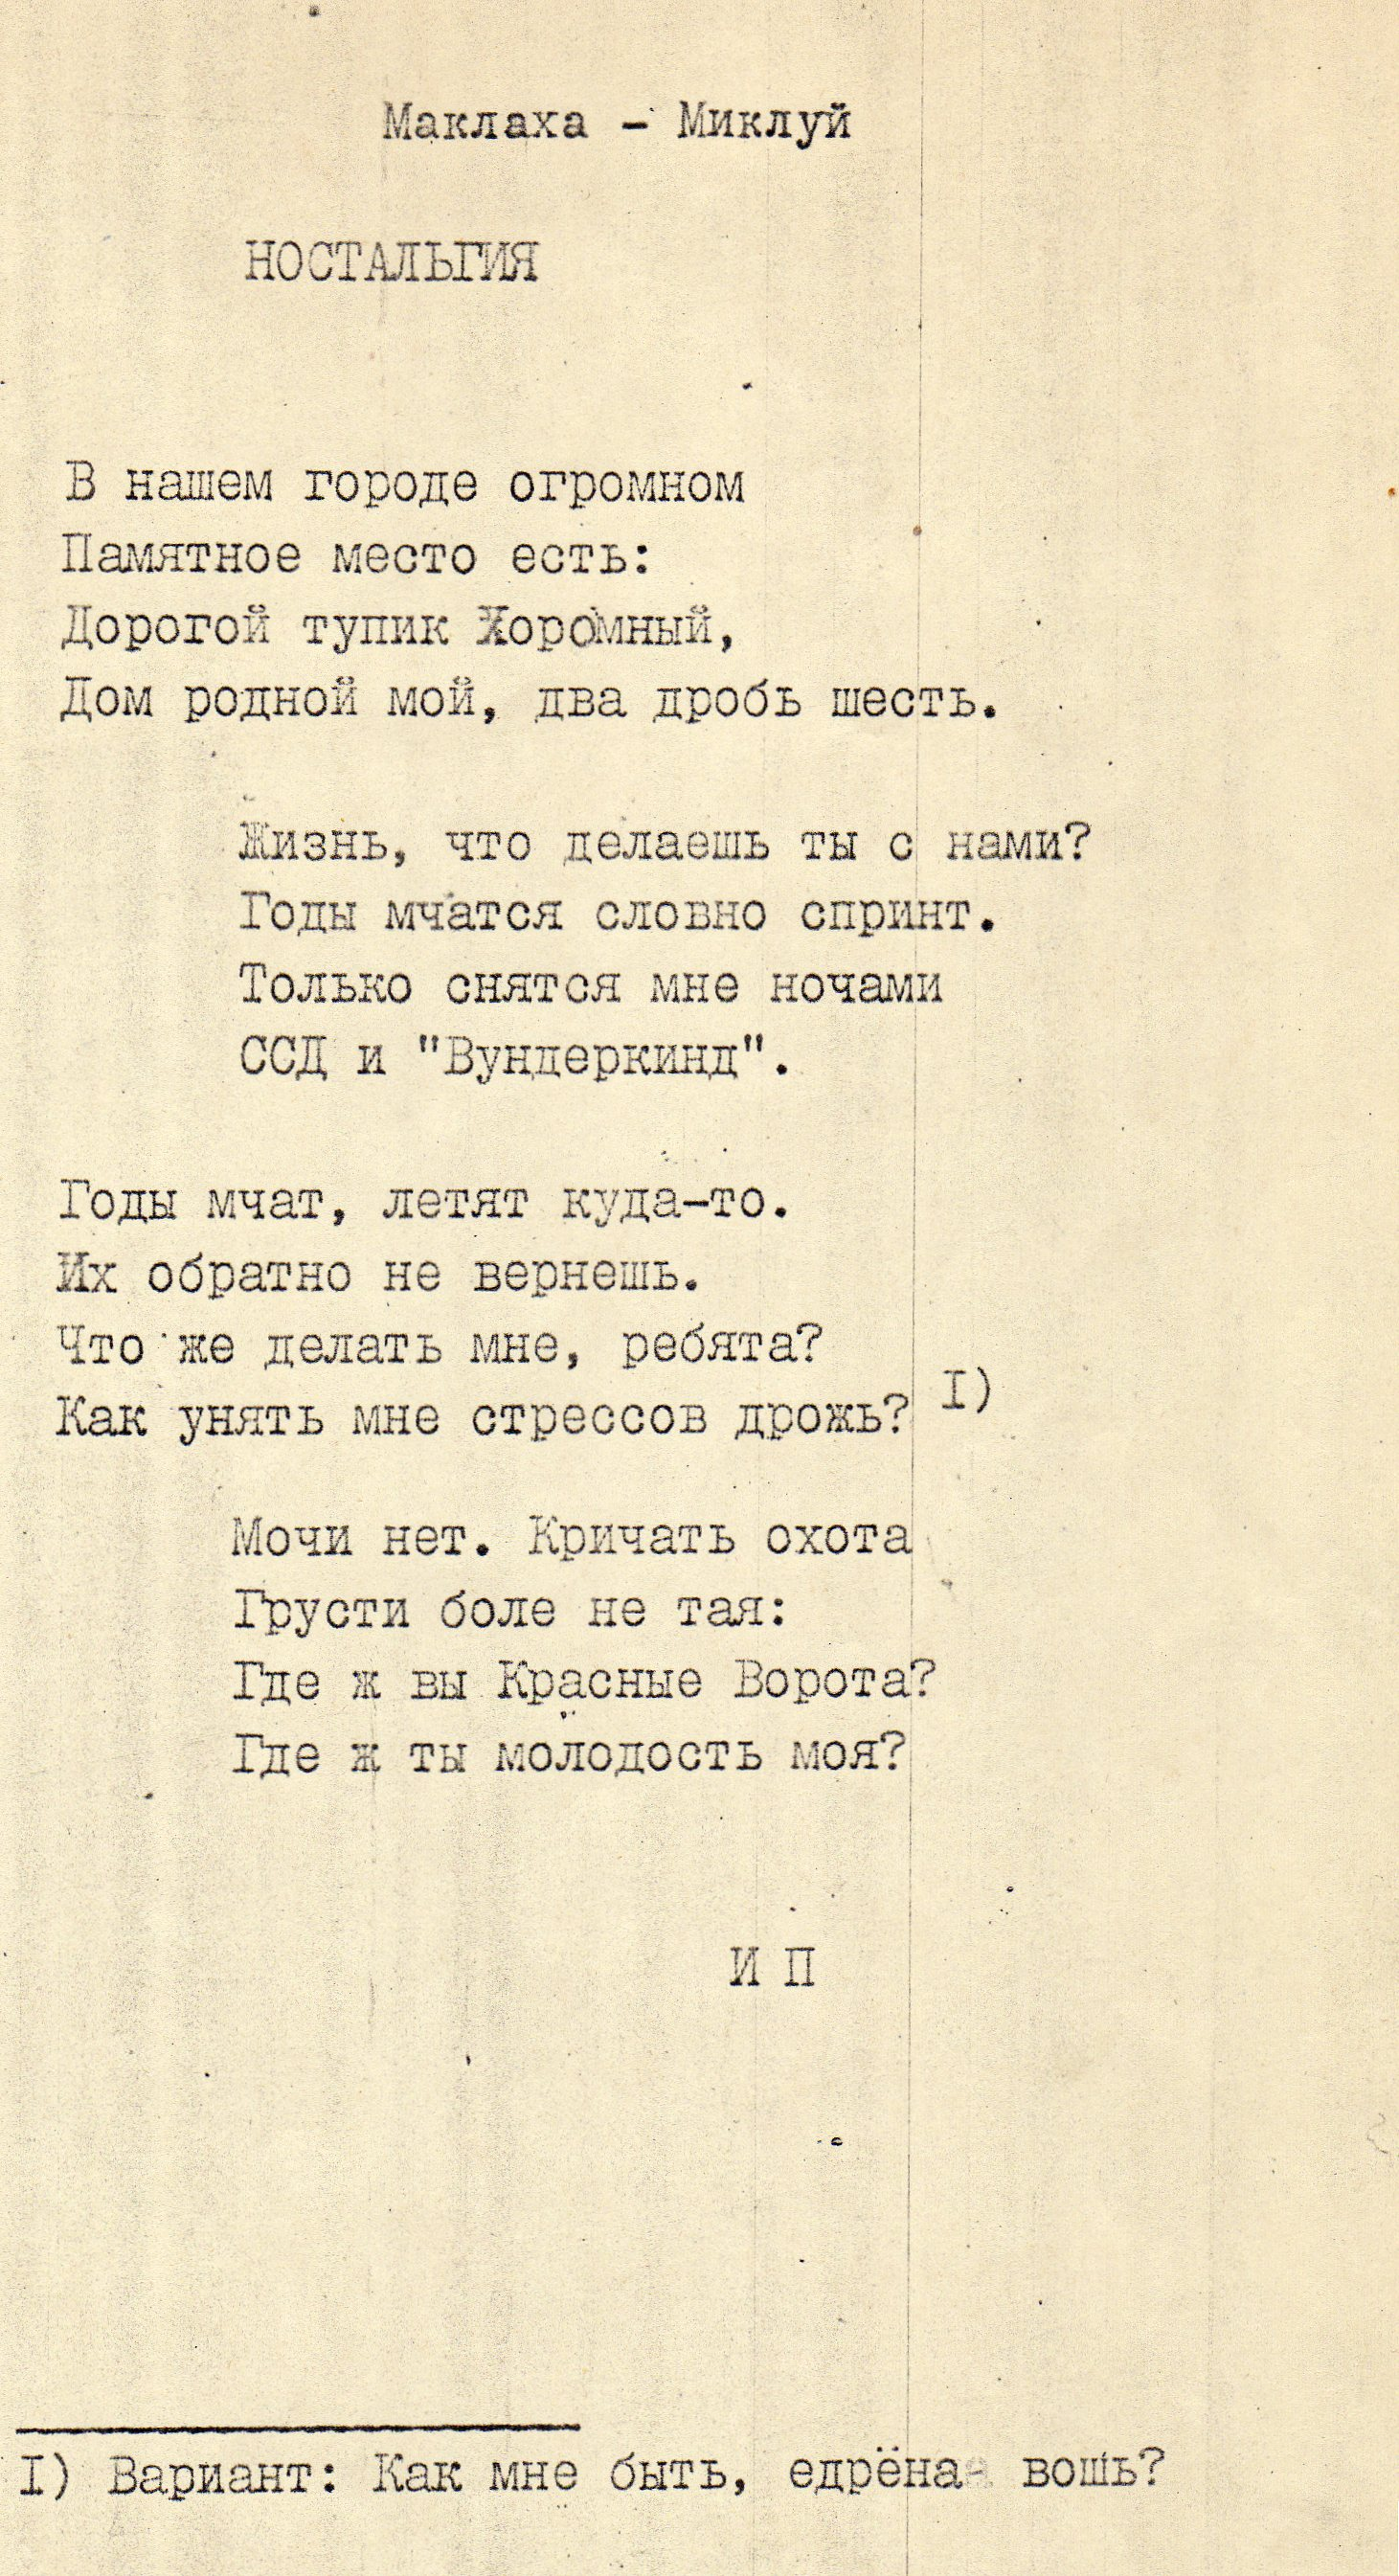
\includegraphics[width=\textwidth]{inc/Vynd/Vynd021}

\noindent
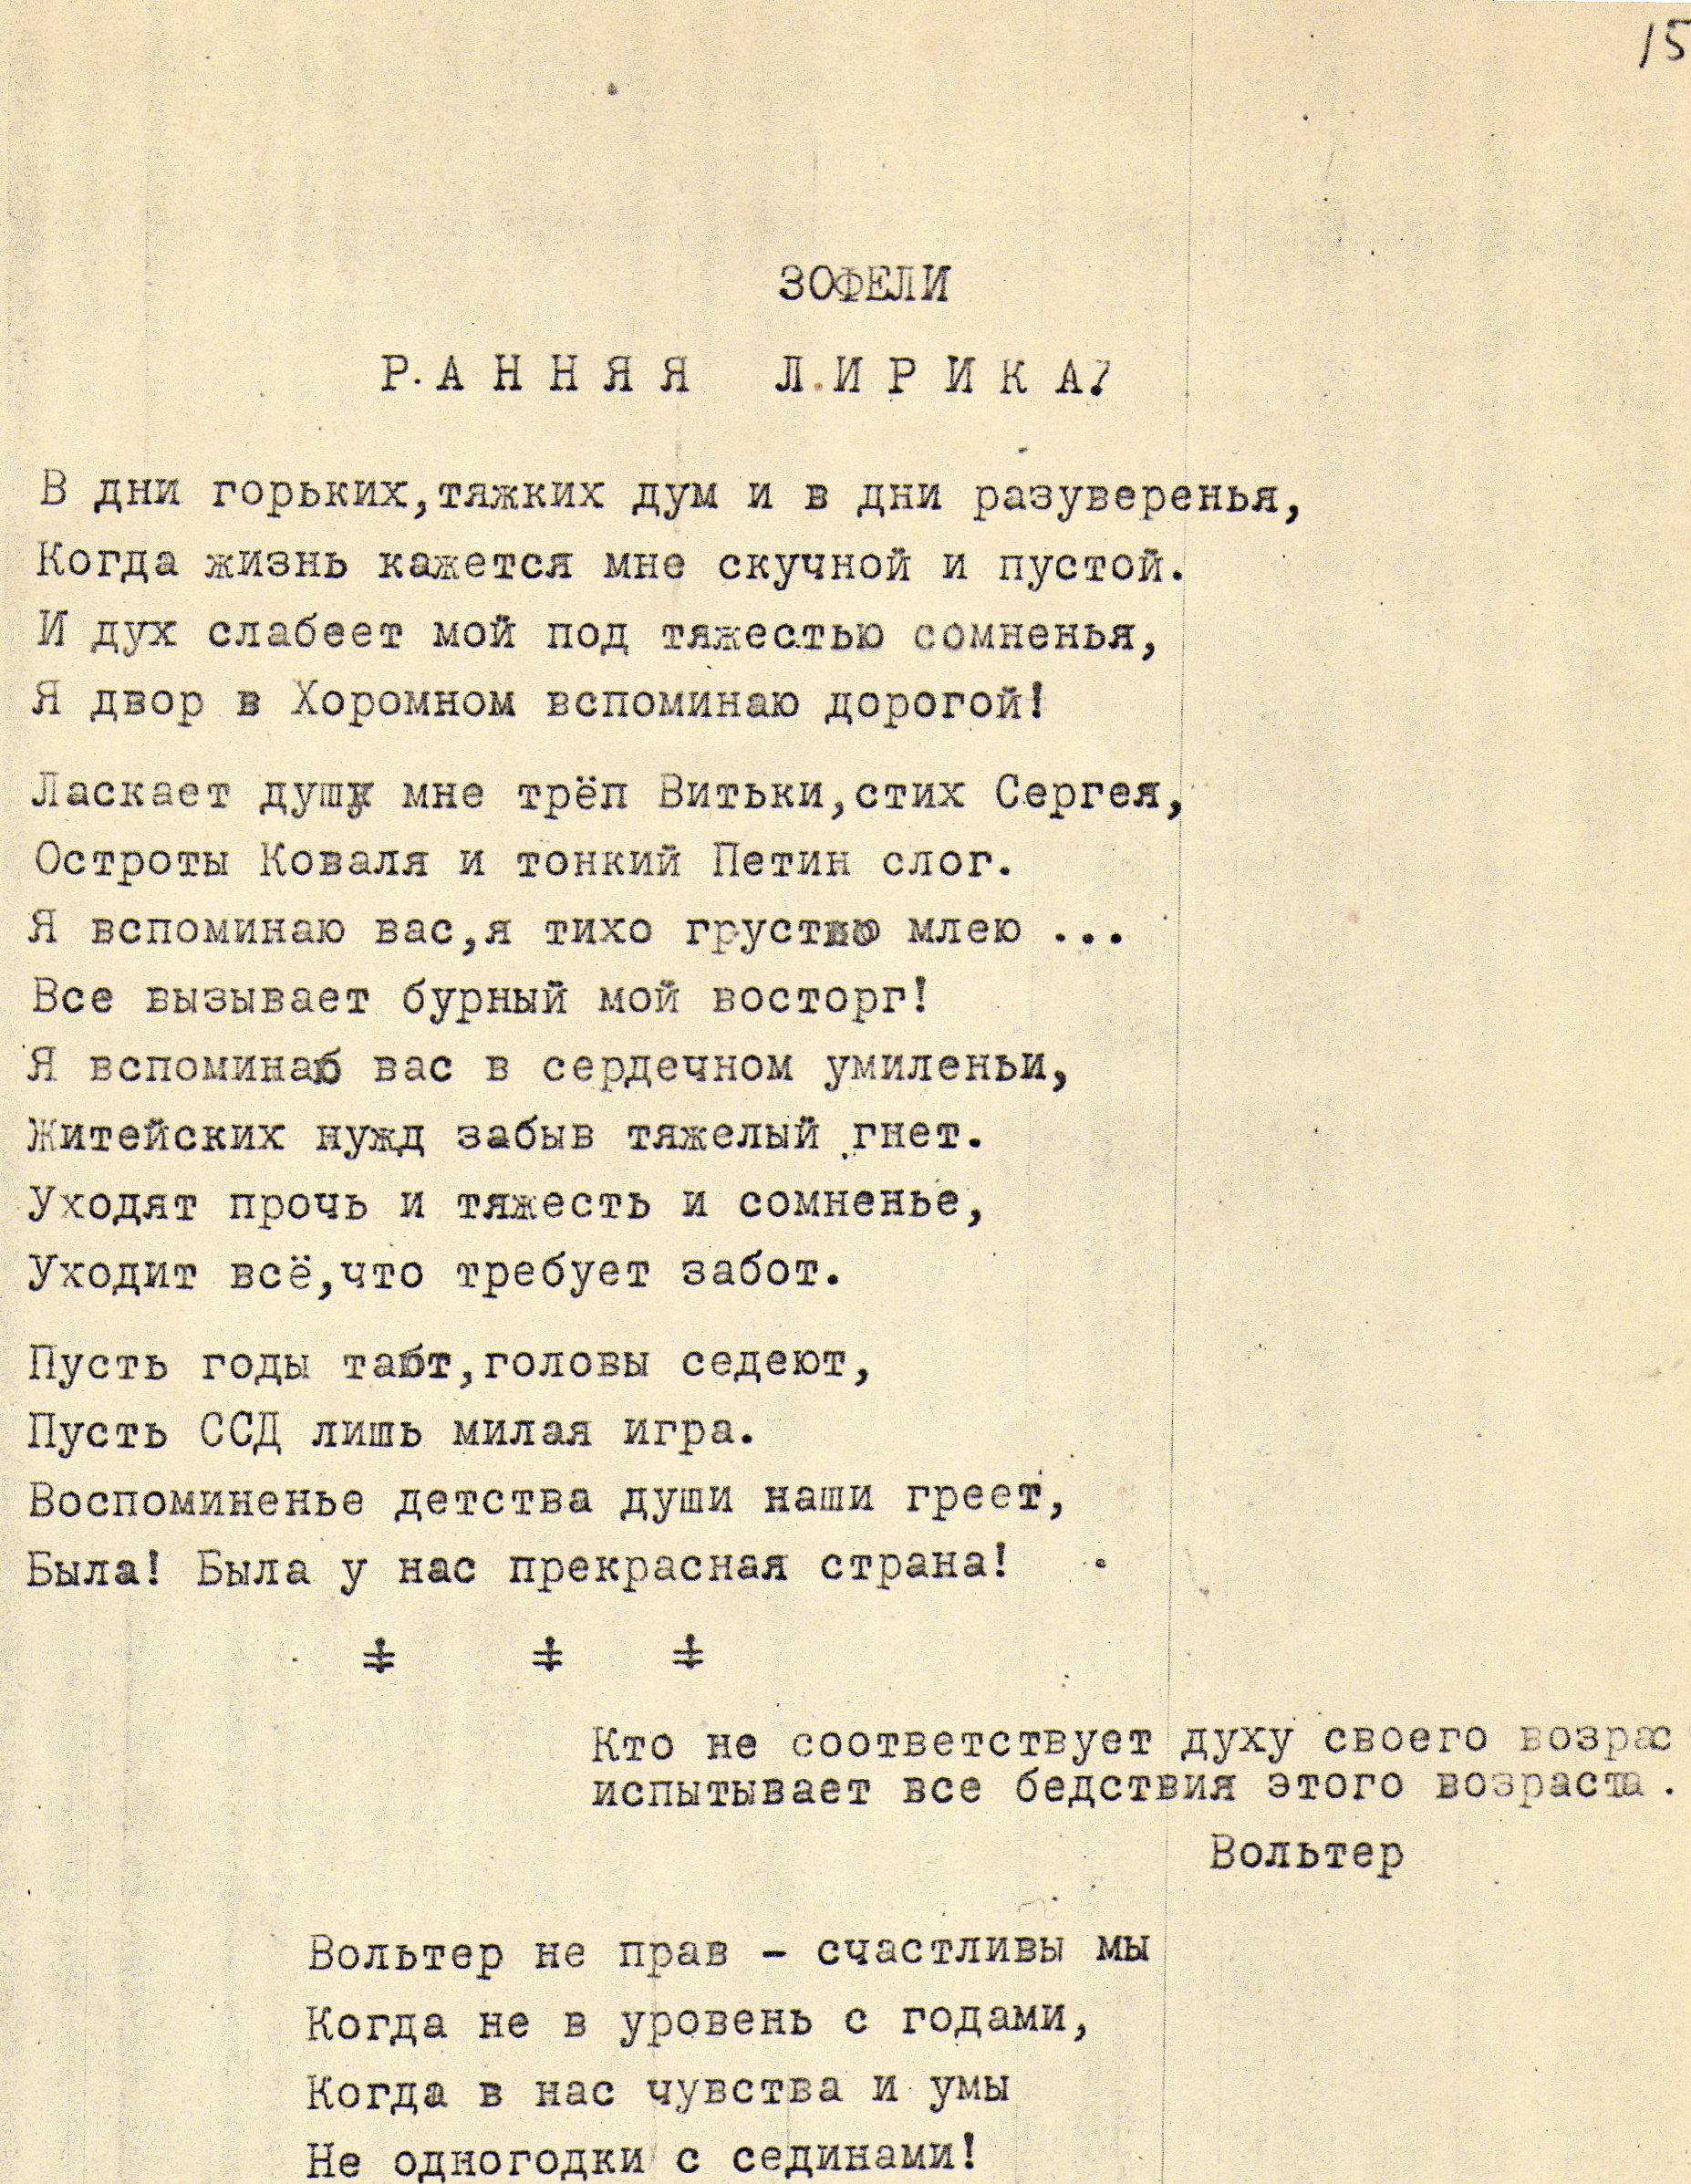
\includegraphics[width=\textwidth]{inc/Vynd/Vynd022}

\noindent
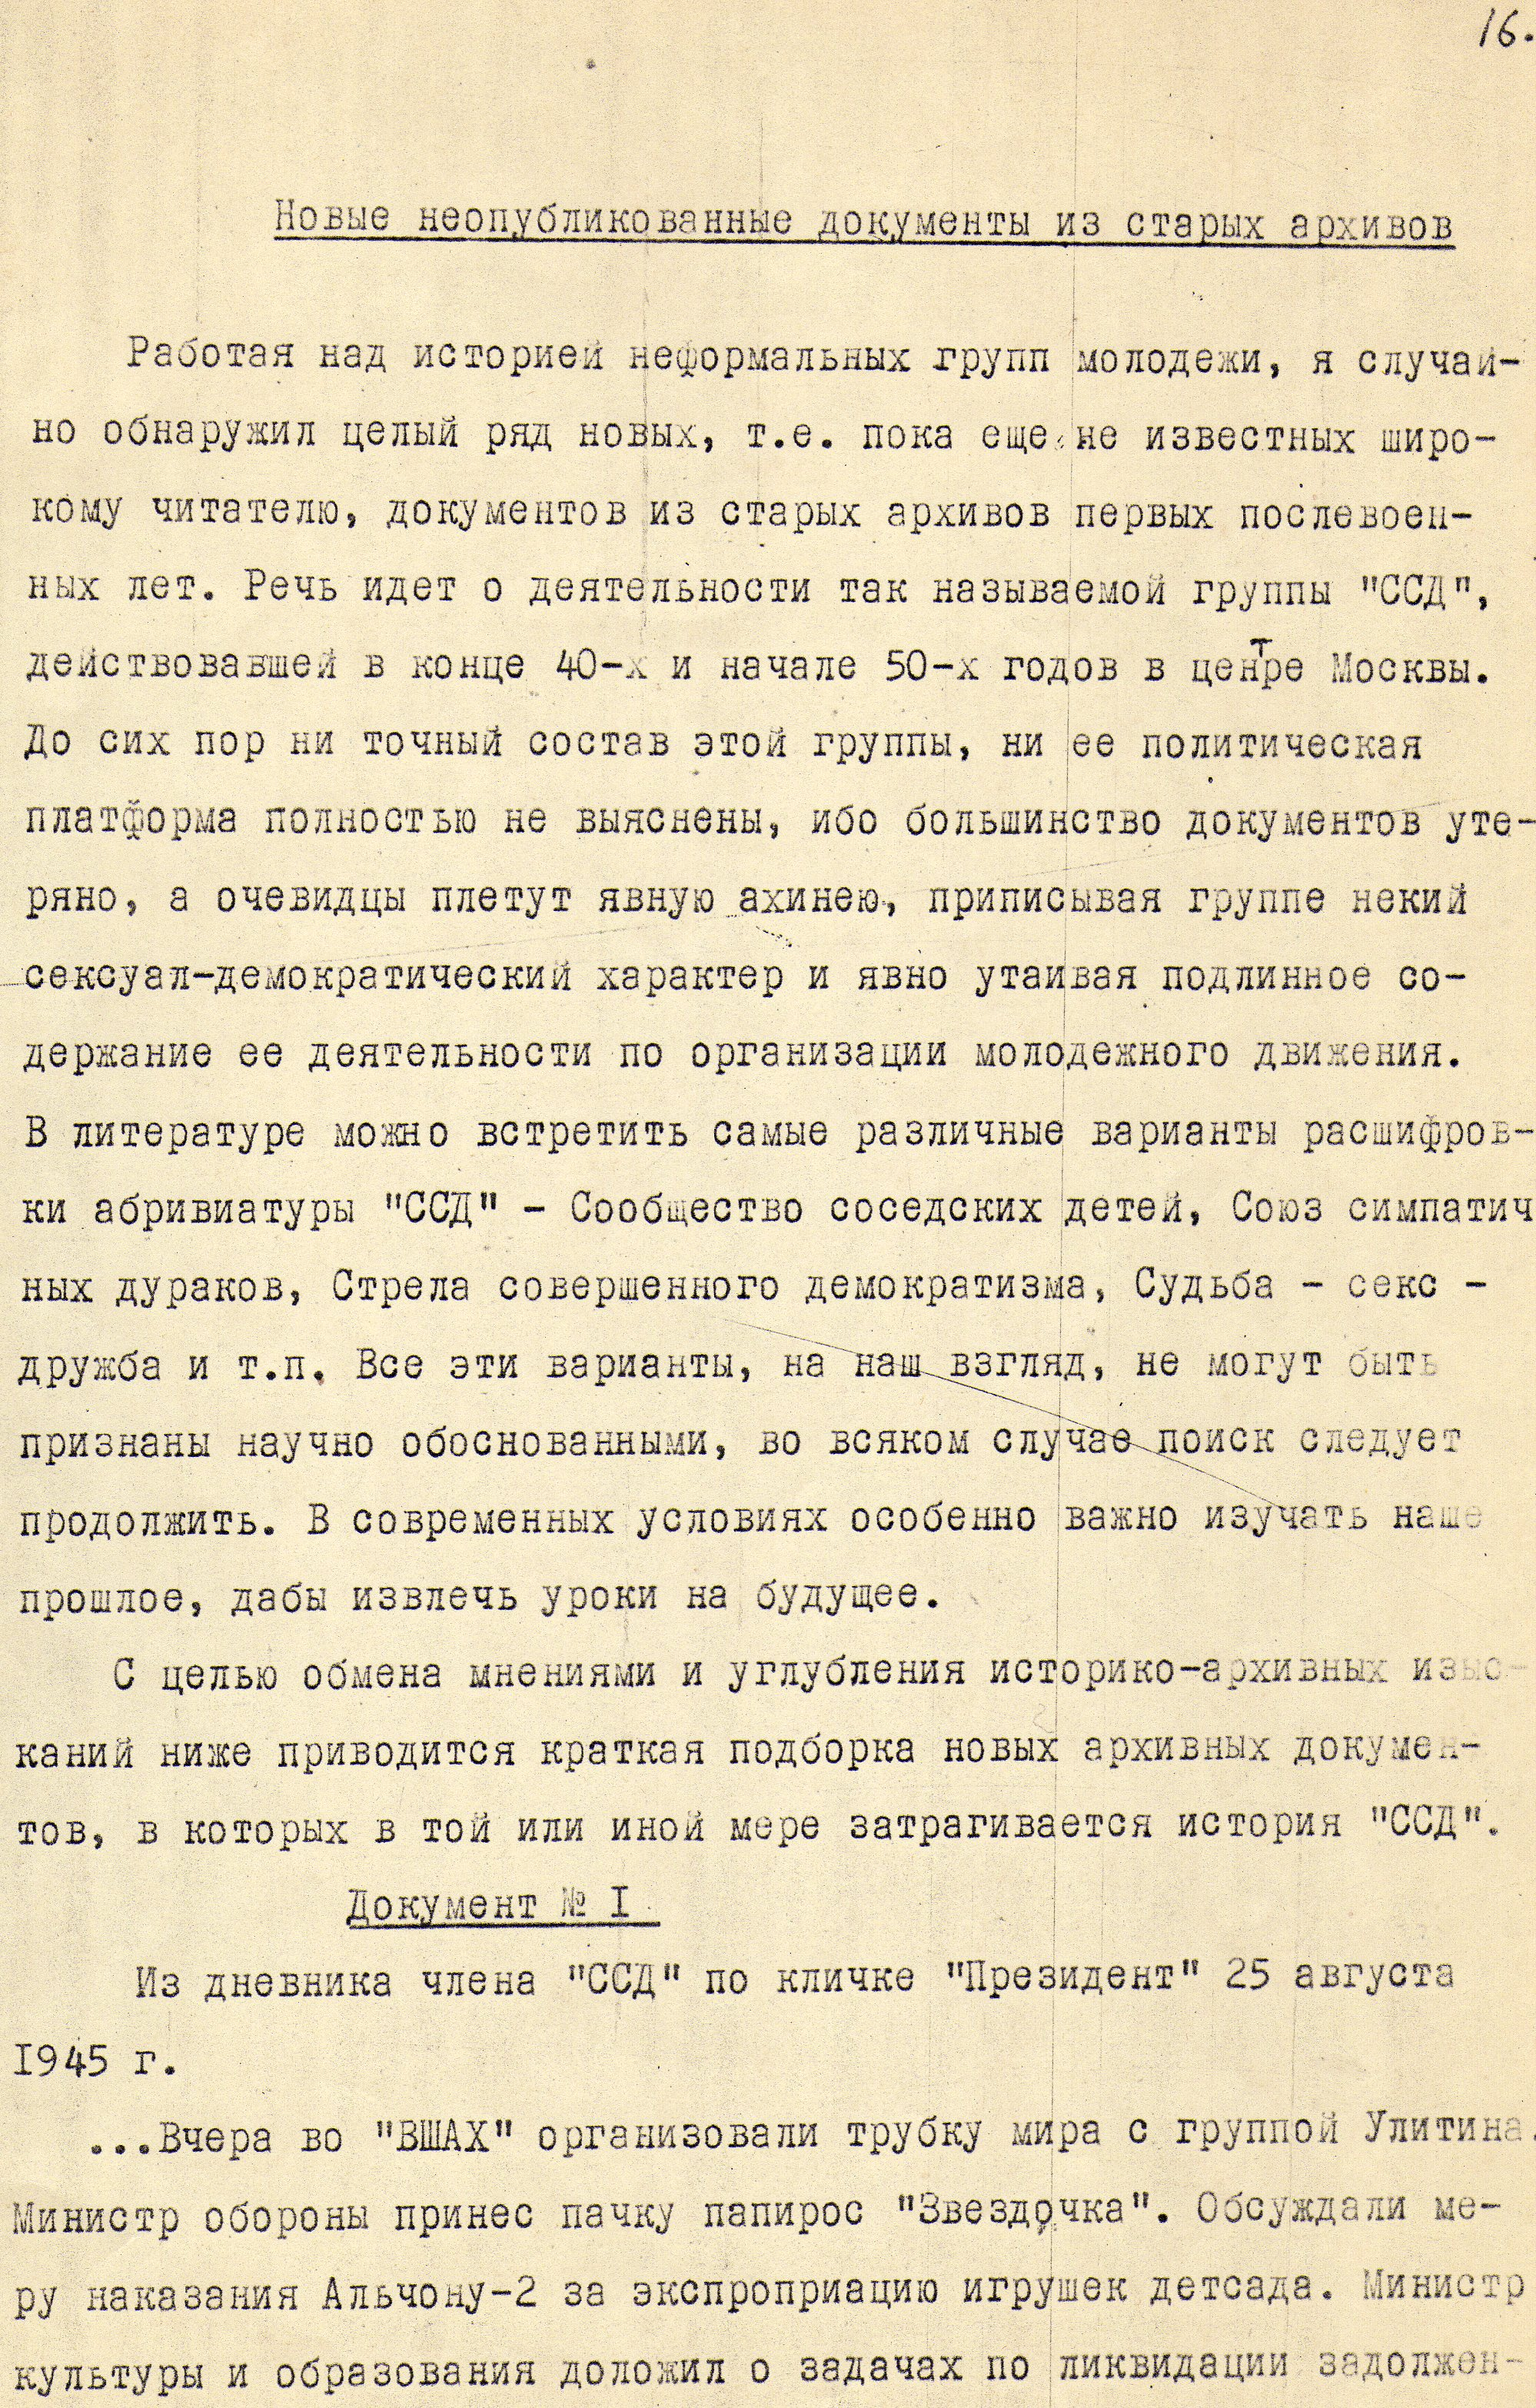
\includegraphics[width=\textwidth]{inc/Vynd/Vynd023}

\noindent
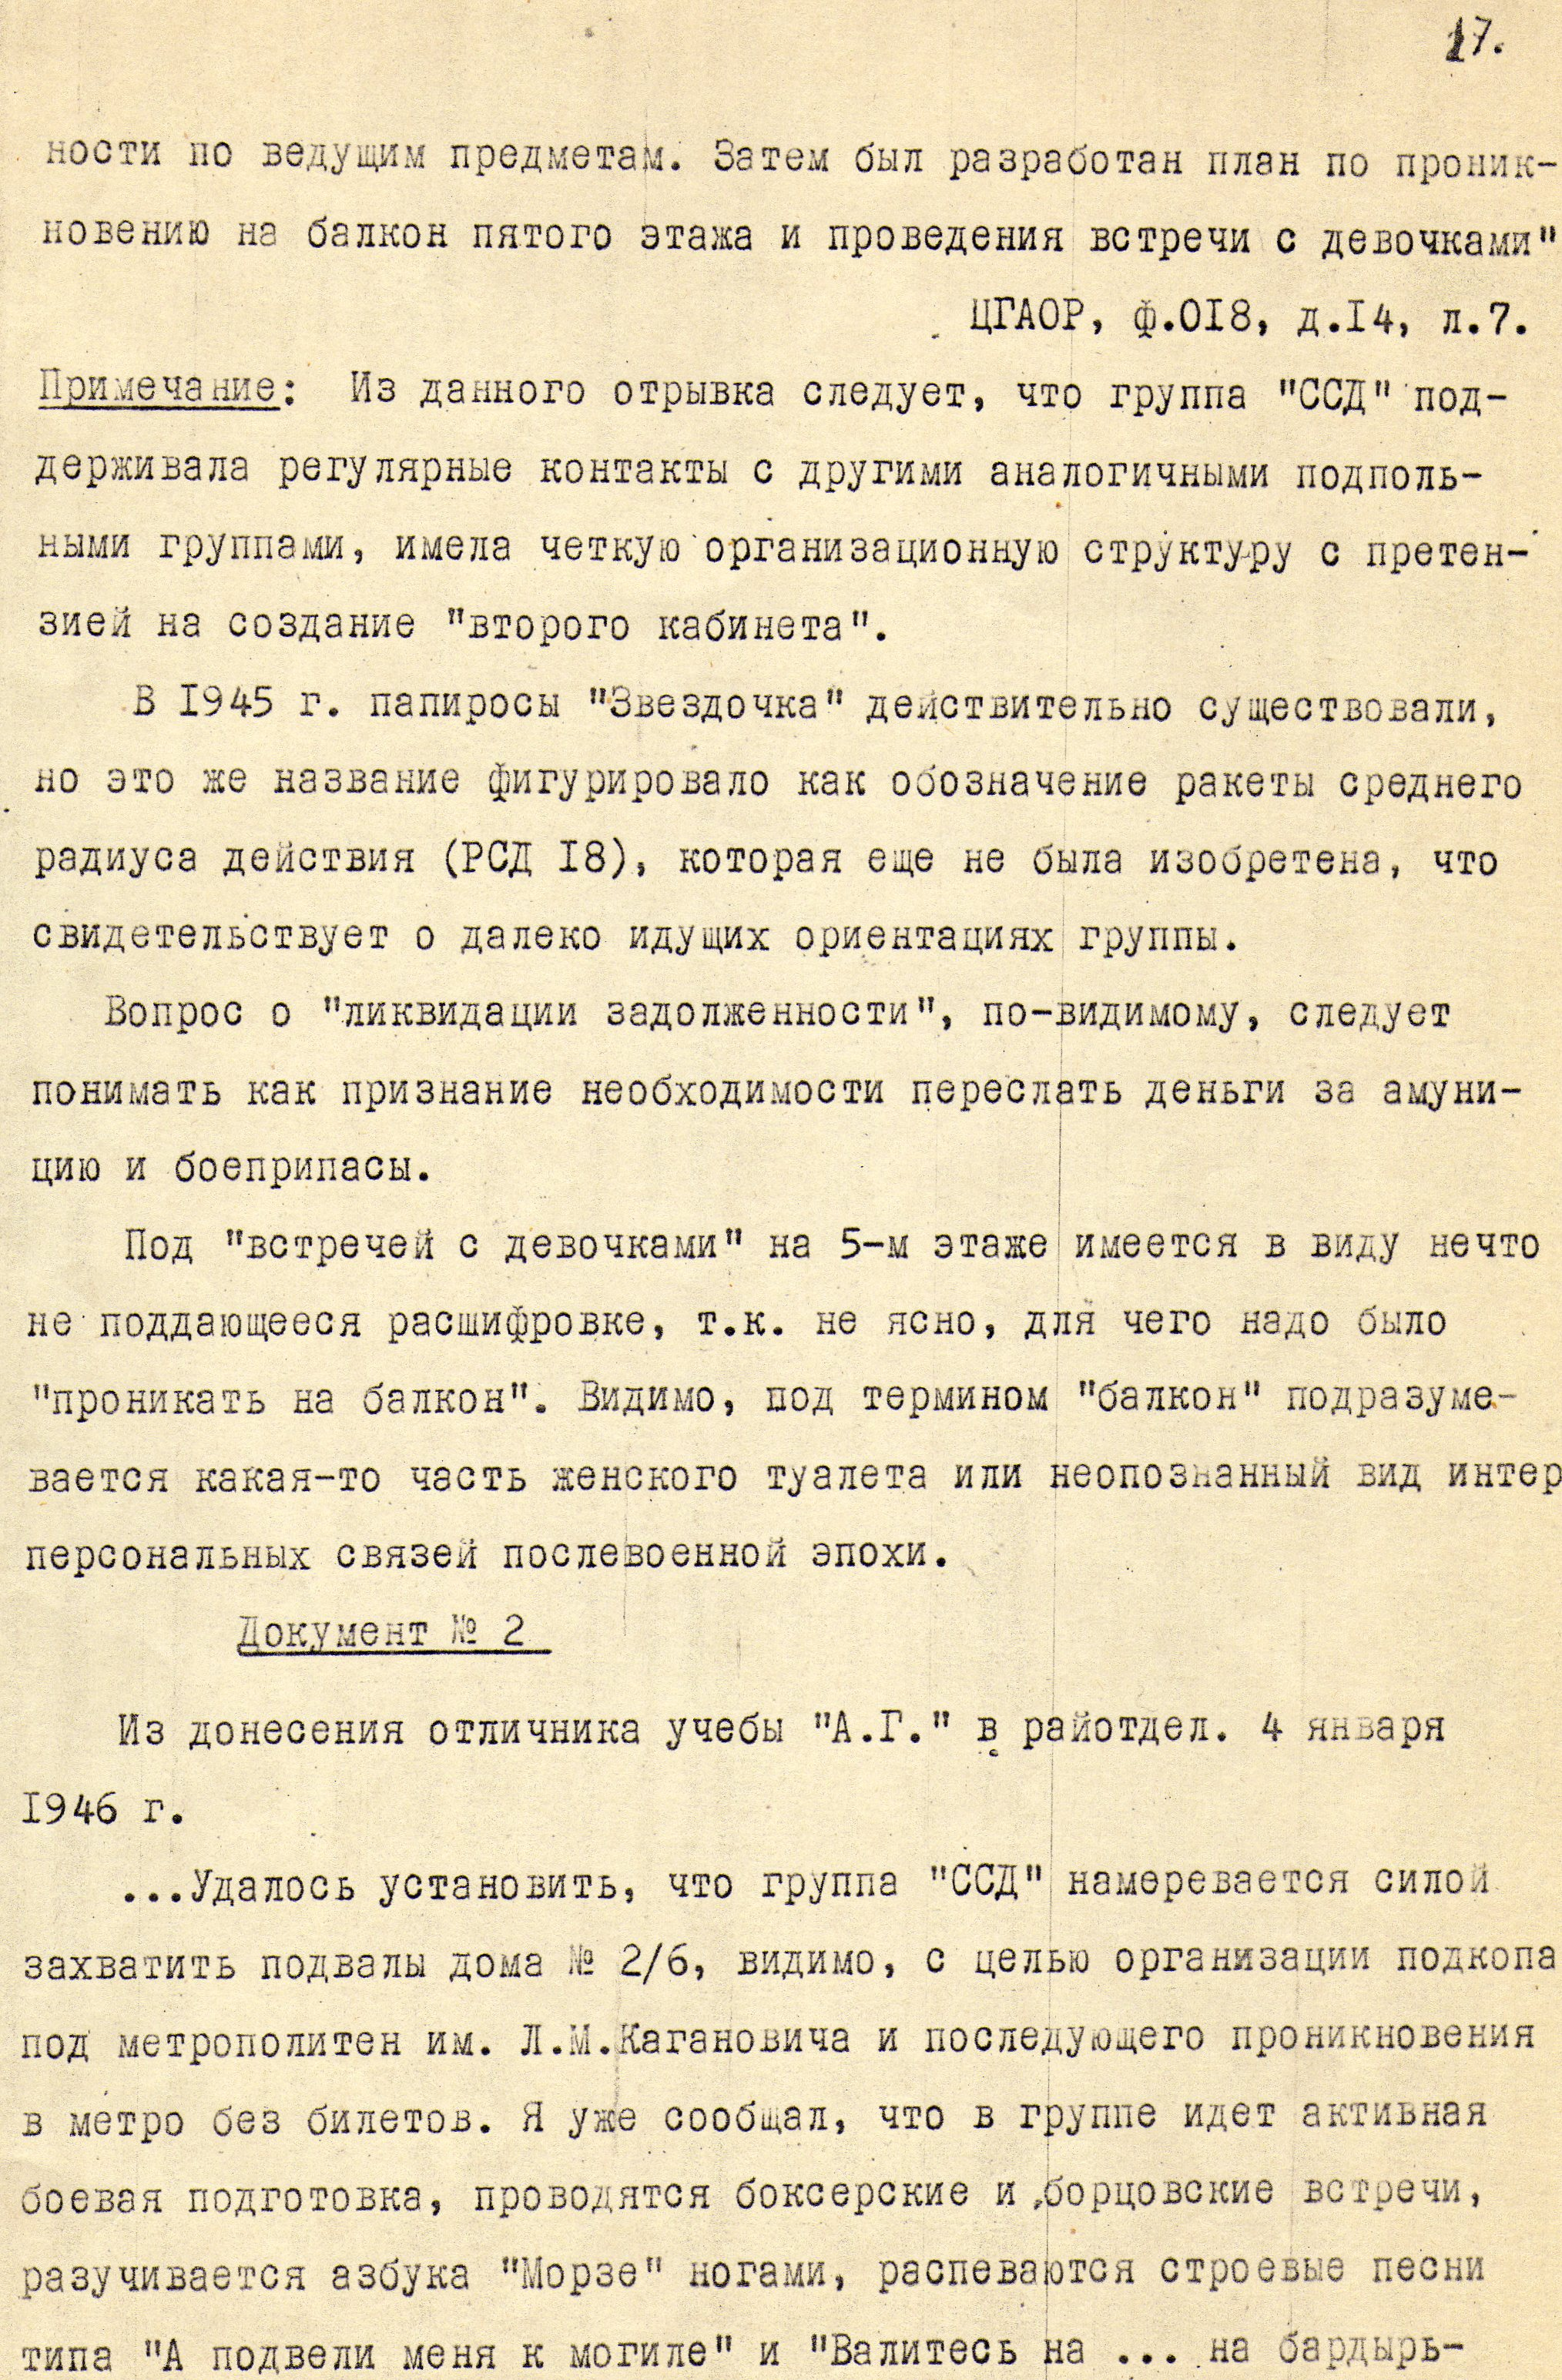
\includegraphics[width=\textwidth]{inc/Vynd/Vynd024}

\noindent
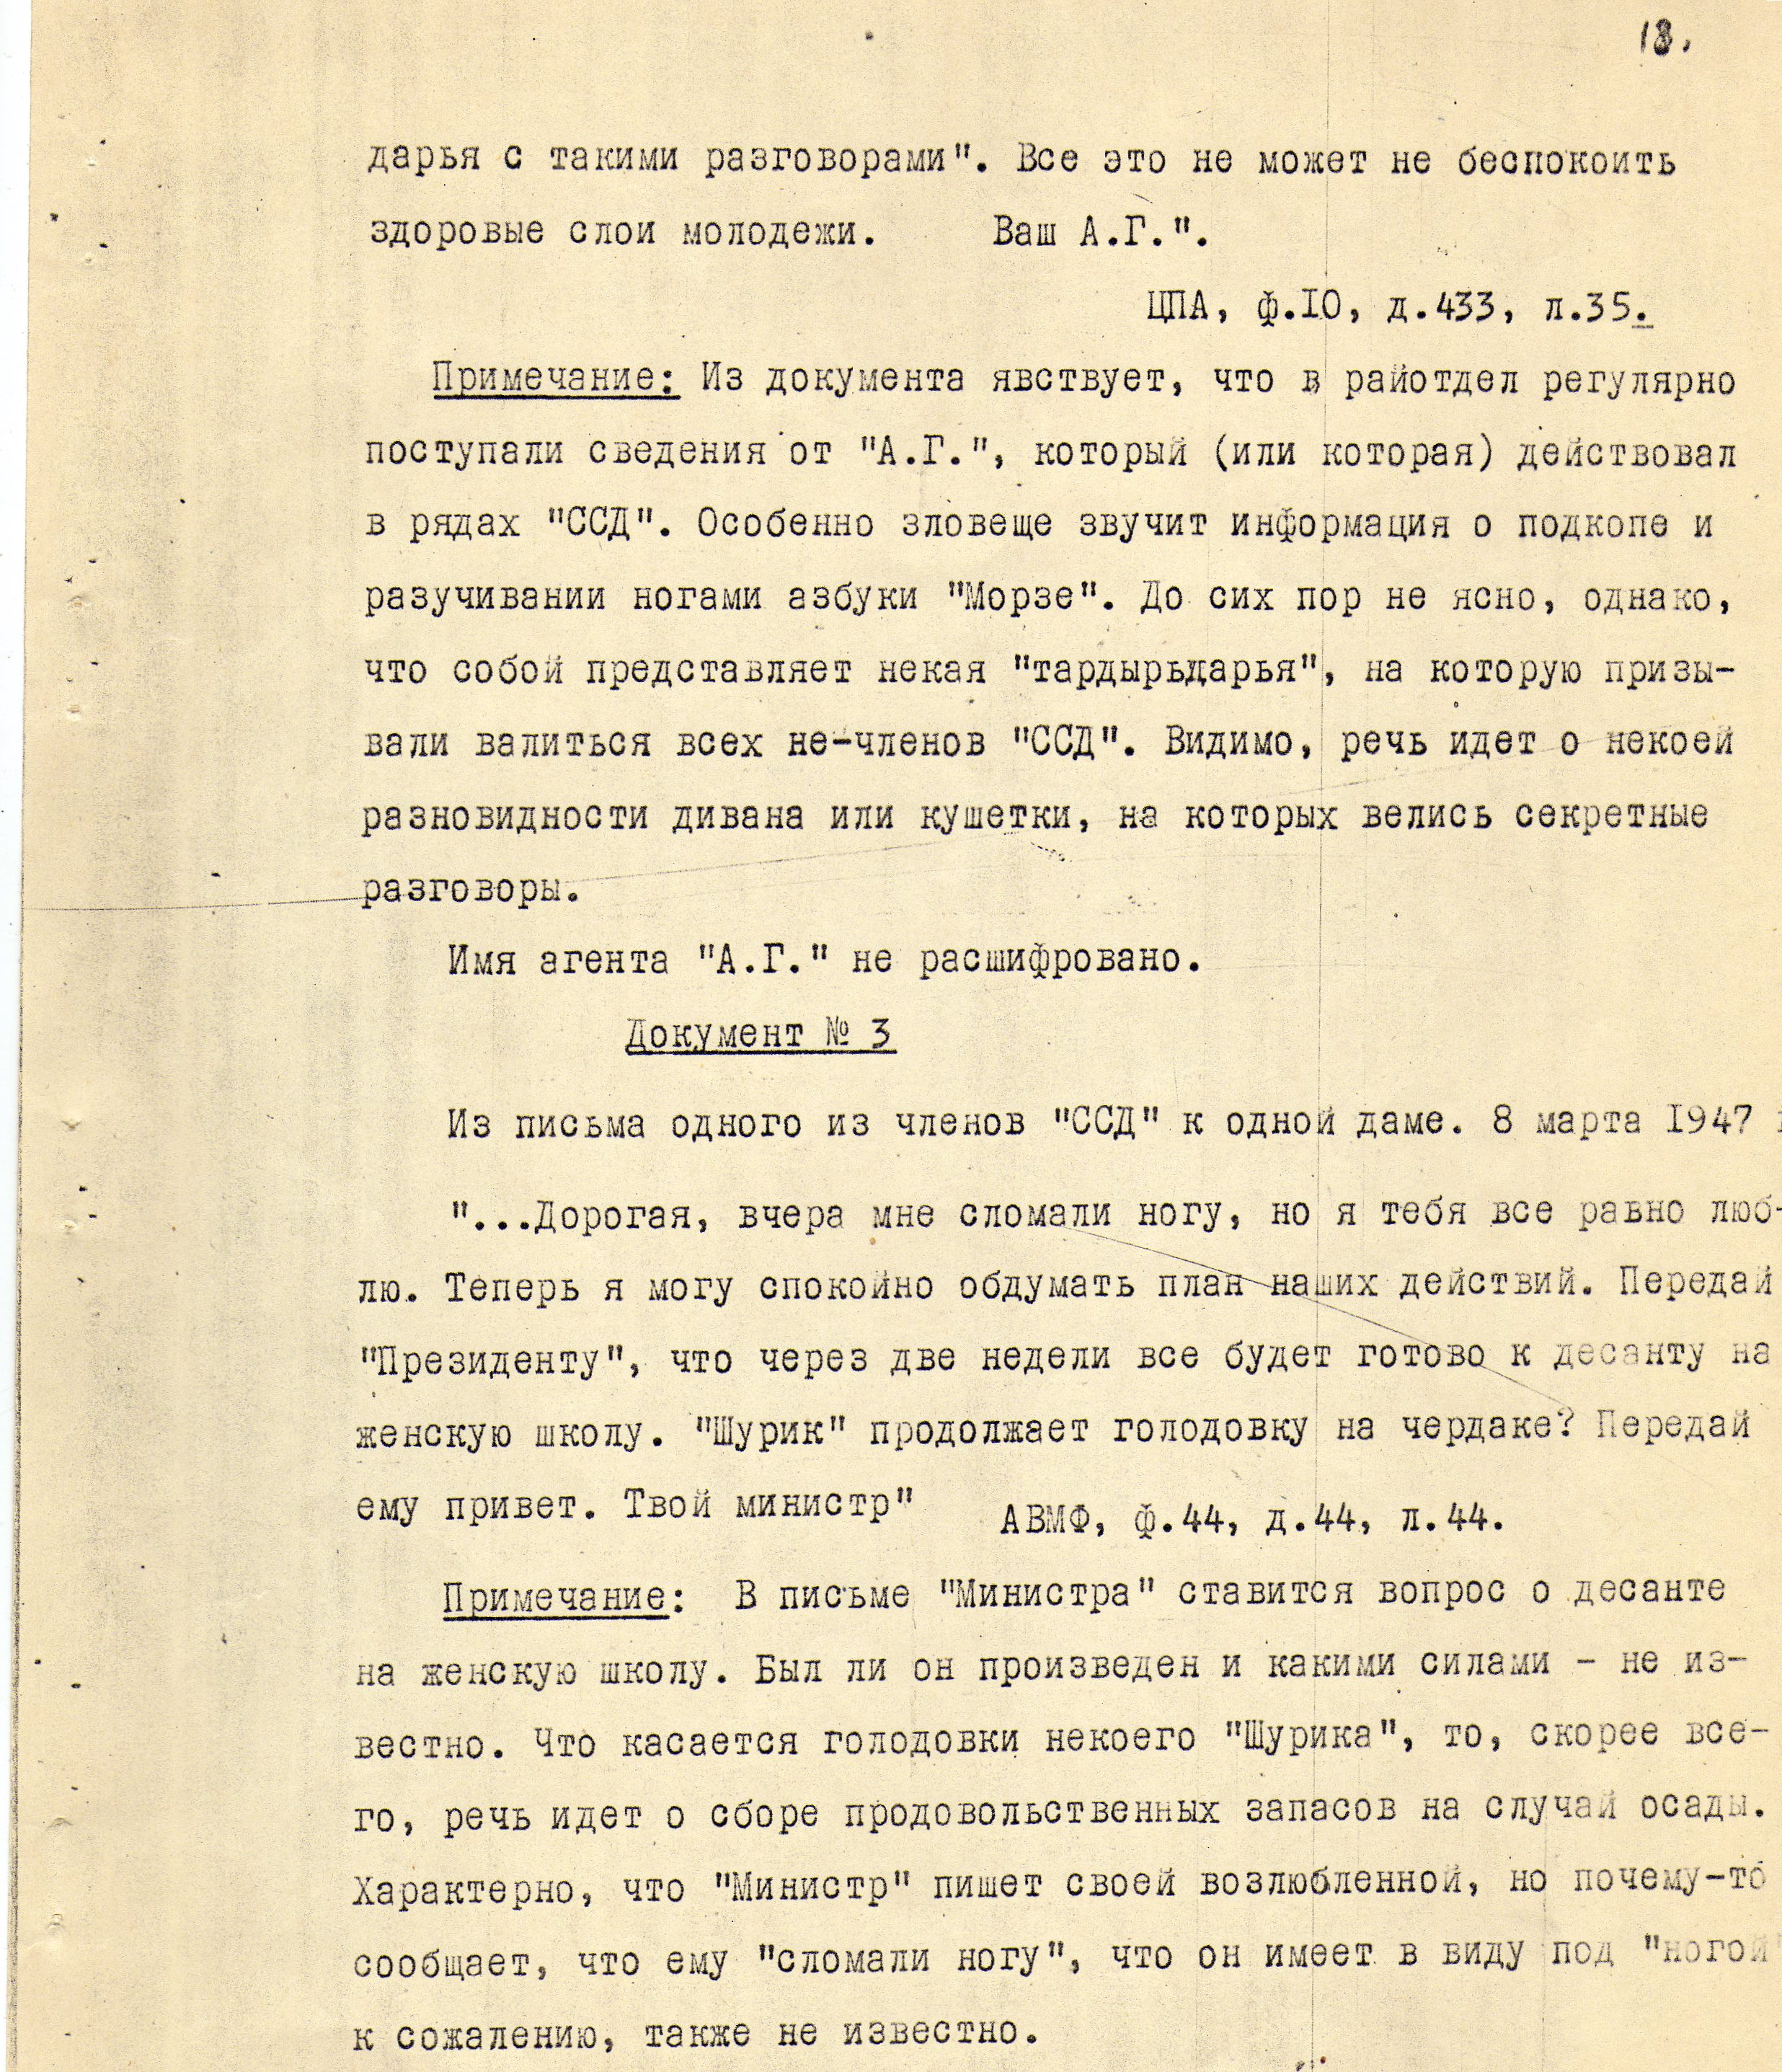
\includegraphics[width=\textwidth]{inc/Vynd/Vynd025}

\noindent
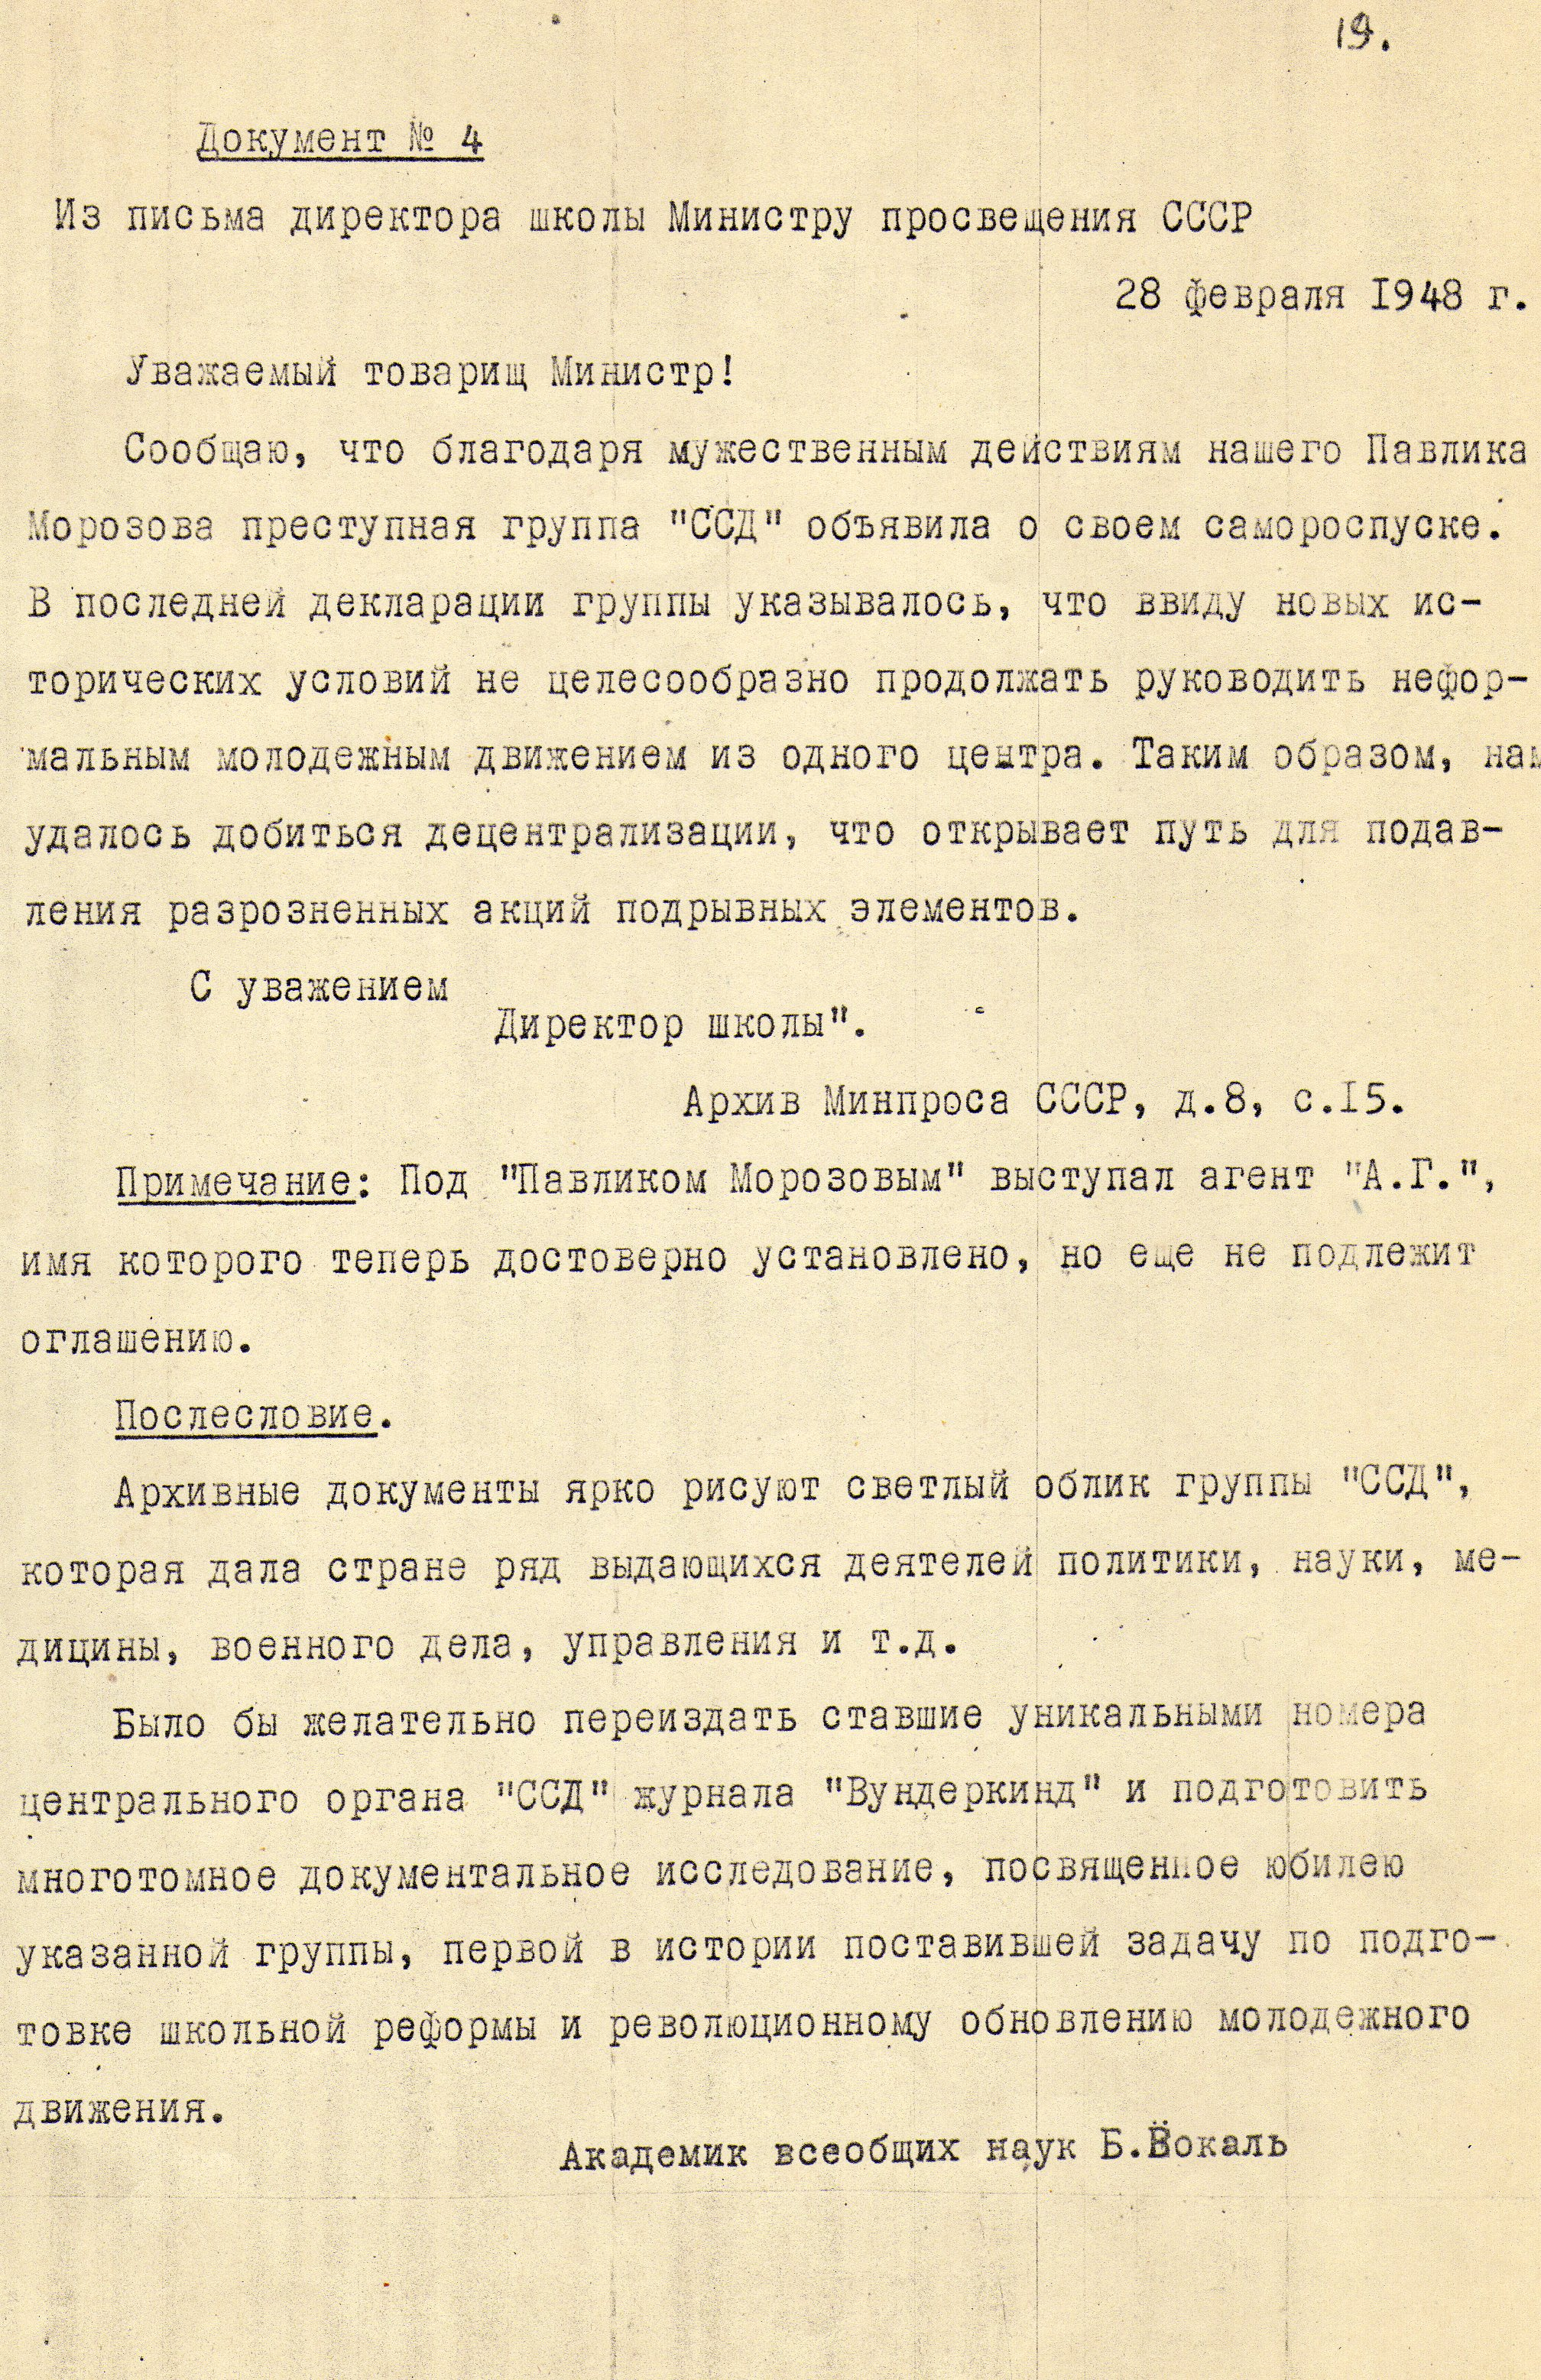
\includegraphics[width=\textwidth]{inc/Vynd/Vynd026}

\noindent
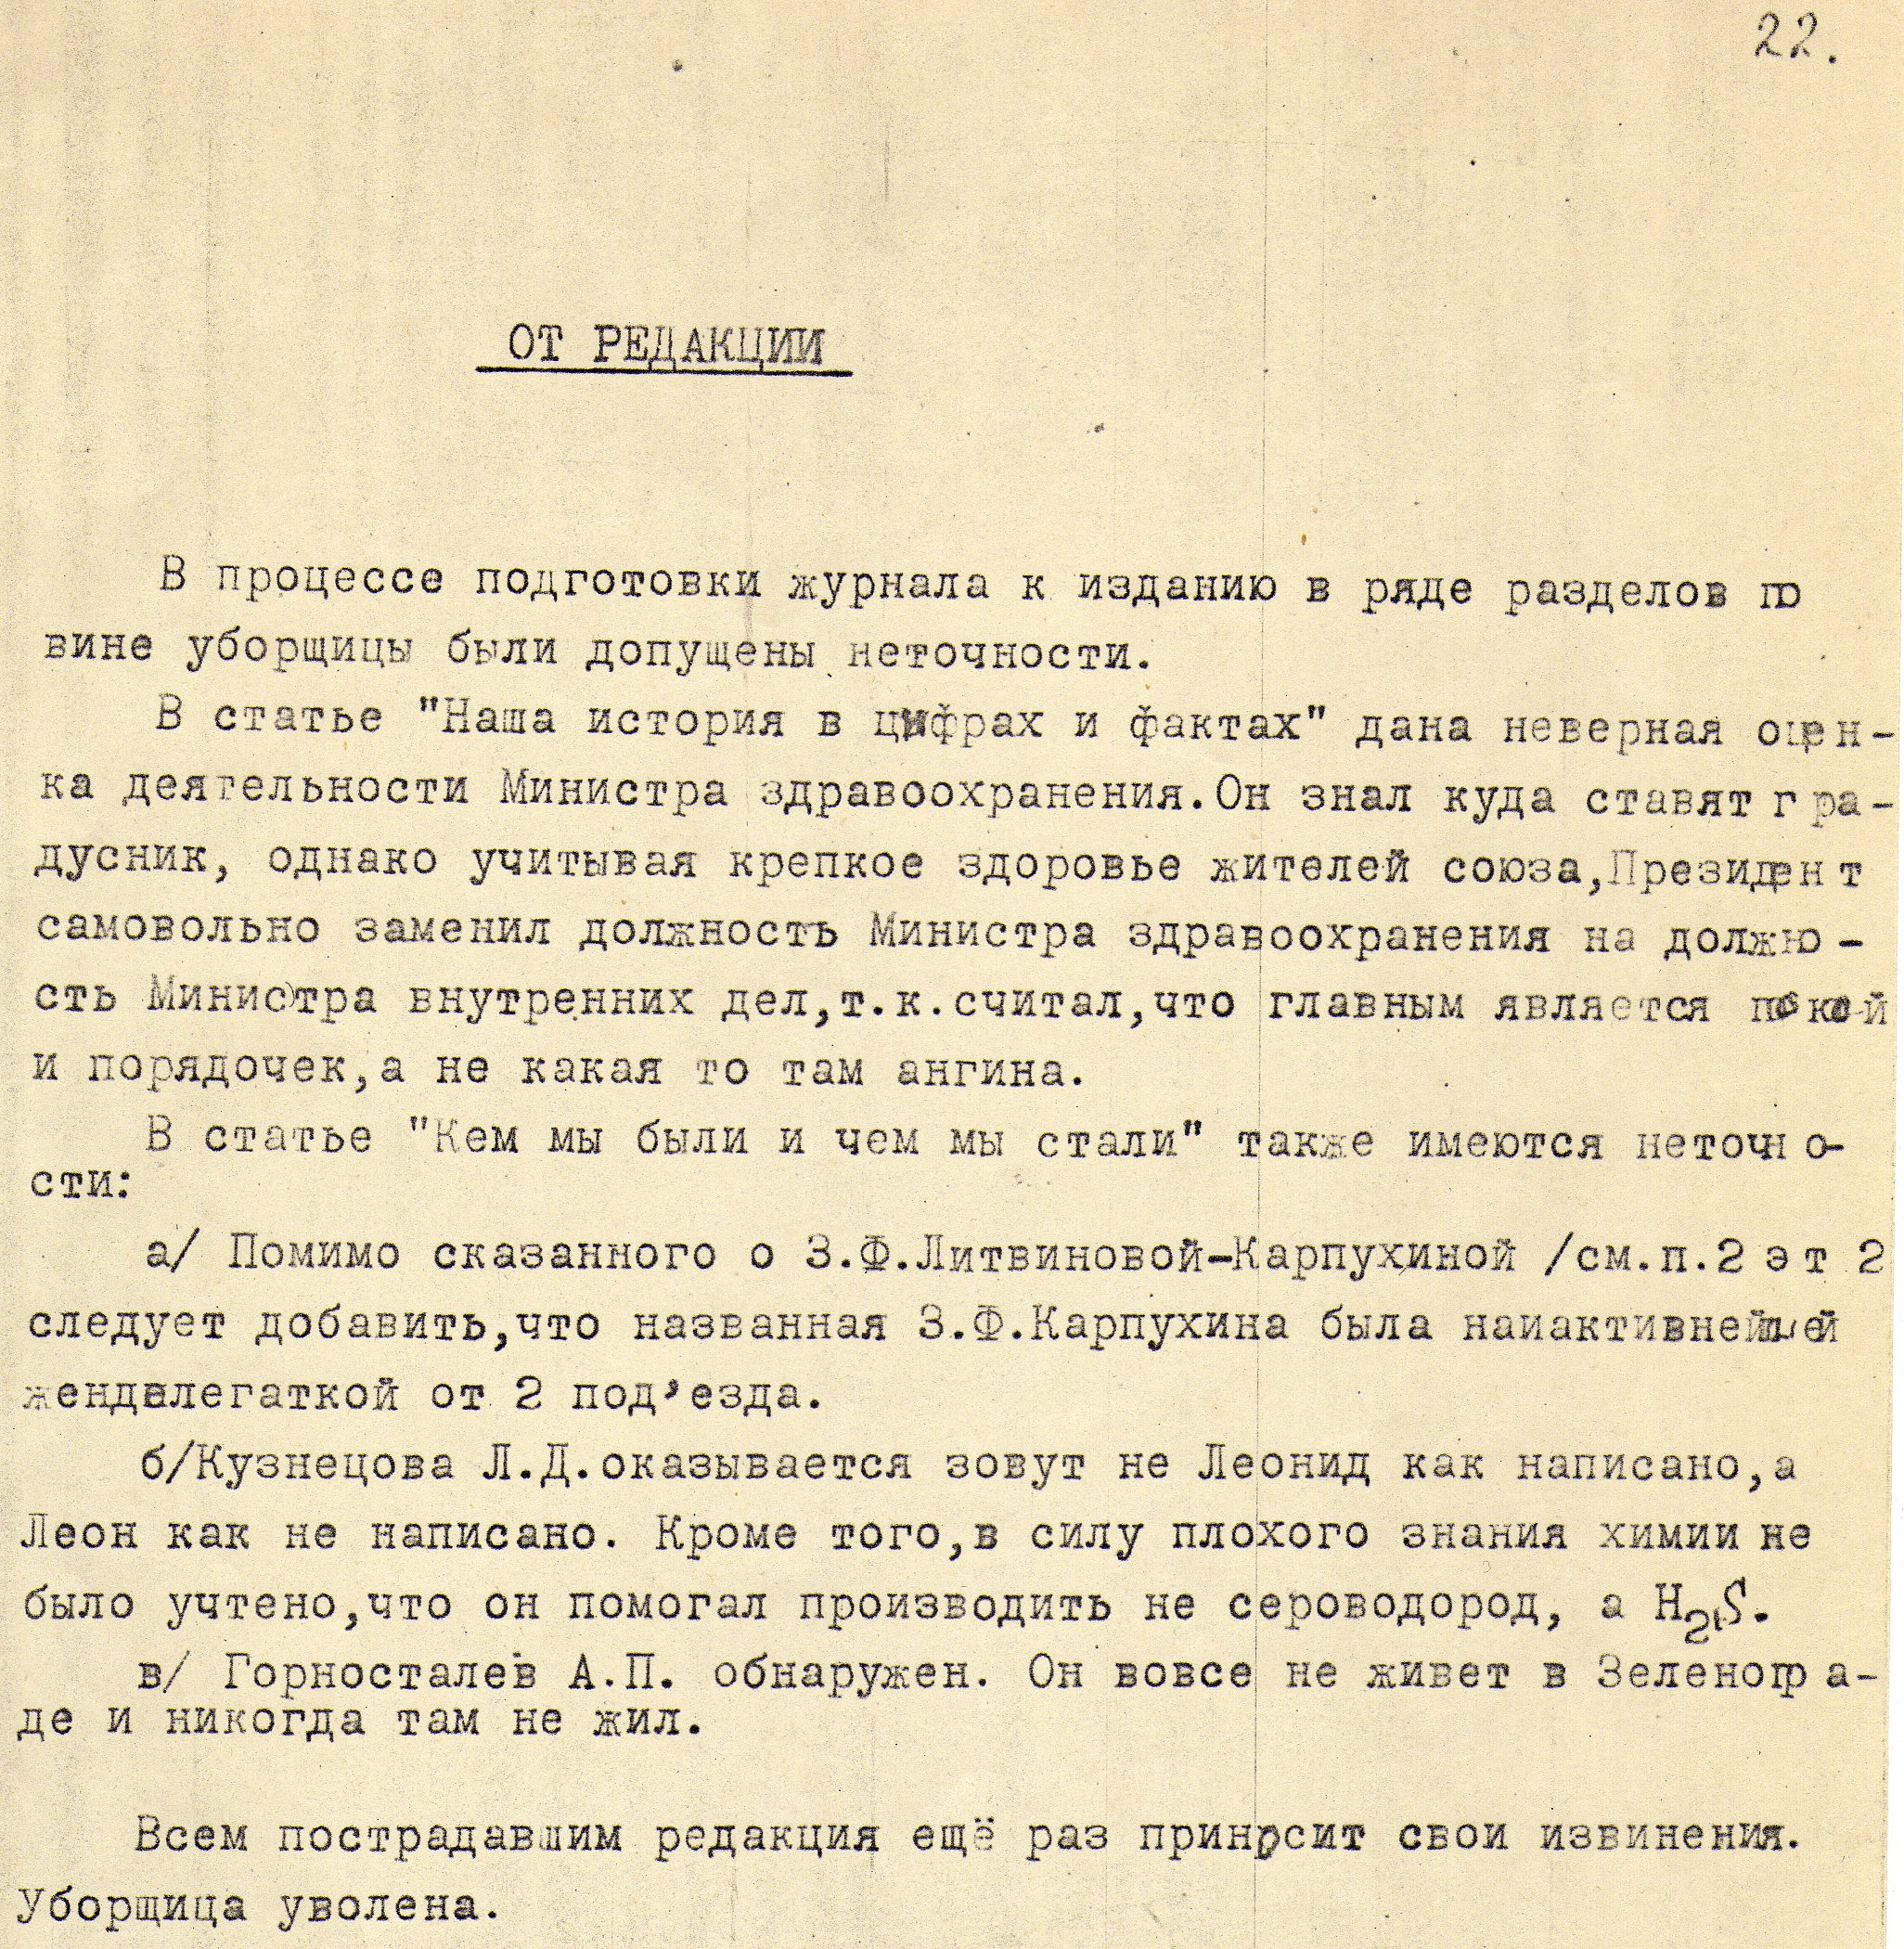
\includegraphics[width=\textwidth]{inc/Vynd/Vynd027}

\noindent
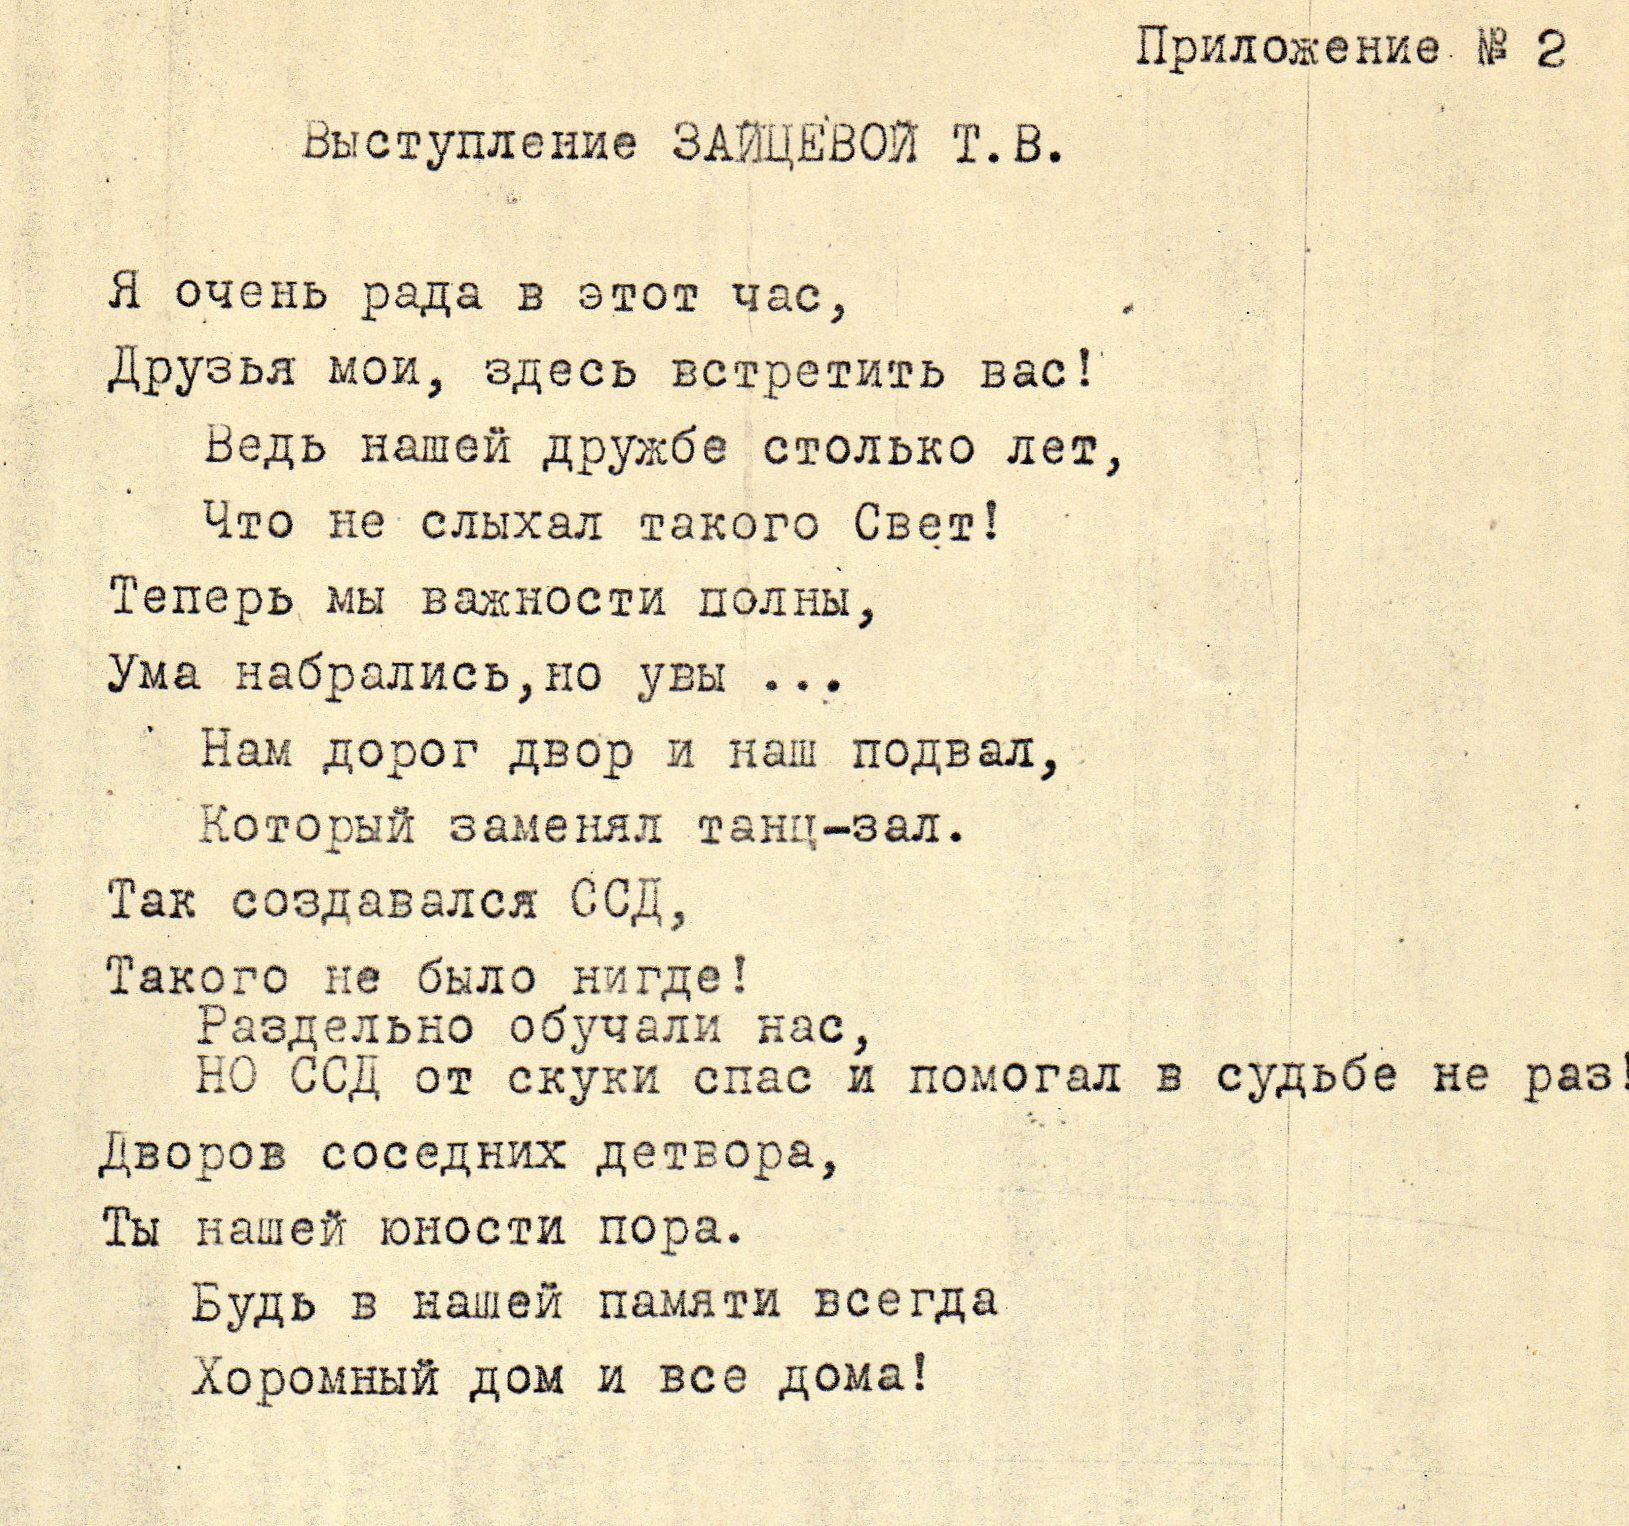
\includegraphics[width=\textwidth]{inc/Vynd/Vynd028}

\restoregeometry



\chapter{}

\section*{Из воспоминаний О. А. Гриневского.}

В детском саду нам было куда как хорошо~-- играли, пели, читали стихи, Конечно же танцевали, наряженные в костюмы, которые носят в разных регионах страны: кто в русских, кто в украинских, кто в узбекских. Ну а я, конечно, в казацкой черкеске с газырями, в папахе, с вытянутыми вдоль плеч руками. А стихи читал даже по украински. Как сейчас помню: 

\indent

{\itshape
Та гей, бикы, чего ж вы сталы! 

Чи поле сильно заросло? 

Чи затупылось чересло?
}

\indent

Так  веселились  в  нашем  детском   саду  Таня  Меньшикова,   Лиля Бирюкова, Ксеня Варзар, Ира Каменская, Нина Уманская, Игорёк Петров, Ленчик Кузнецов, Шурик Штейнберг, Витя Прейс и я~-- звали меня Альчон. 

\indent

\begin{center} 
    * * *
\end{center}

\indent

Но главным местом, где шла моя адаптация к новой жизни, был наш двор в доме у Красных ворот. В 1943 году из старой детсадовской компании там оставались Таня Меньшикова, Ксеня Варзар, Ира Каменская, Лиля Бирюкова, Витя Прейс, Игорь Петров и я. Зато стали появляться новые друзья~-- Сережа Дивильковский, Борис Коваль, Зоя Карпухина, Алик Горносталев, Шурик Штеинберг, Ленчик Кузнецов, Володя Литвинов, Люция и Коля Фроловы. И постепенно этот круг друзей расширялся.

Жили мы дружно и после школы постоянно собирались у нас во дворе. Этому немало способствовал и сам наш дом, построенный в виде подковы, которая упирается в стену дома № 4, что в Боярском переулке. Поэтому двор внутри подковы -замкнутое пространство. Вход в него через ворота со стороны, которая выходит к площади у Красных ворот. Вокруг двора рассажены деревья, а посредине~-- фонтанчик, из которого тихо стекала вода. В общем, лучшего места для общения и игр не придумаешь.

А из наших дворовых игр прежде всего вспоминаются «салочки», «колдунчики», «прятки» и «казаки~-- разбойники». Были считалки на тарабарском языке тех детских лет. Например: «Эни, бэни, ряба, квинтер, финтер, жаба...». Или:

\indent

{\itshape
«Дора, дора --помидора,

 Во дворе поймали вора,
 
  Стали думать и гадать,
  
Как бы вора наказать.

Мы связали руки -ноги
 
И пустили по дороге. 

Вор шёл, шёл 

И корзиночку нашел. 

В этой маленькой корзинке 

Есть помада и духи, 

Ленты, кружева, ботинки
 
--Что угодно для души».

}

\indent

Наиболее азартной и массовой игрой были «казаки и разбойники». Мы делились на две группы, одна из которых~--разбойники~-- убегали, а другая~-- казаки~-- должны были их ловить. При этом разбойникам представлялось время, чтобы убежать, а затем начиналась ловля.

Была также очень популярная игра в «штандер»,~-- видимо, типично городская и, судя по названию,~-- немецкого происхождения. Водящий подкидывал и ловил мячик, и после этого кричал~-- штандер! Все разбегавшиеся должны были тут же остановиться и замереть, а водящий по своему усмотрению выбирал жертву, в которую кидал мячик. В случае попадания она и становилась очередным водящим.

И ещё~-- много занимались спортом: бегали, прыгали, а главное для мальчиков~-- играли в футбол на «стадионе Папанин бридж». Так мы называли приспособленную для такой игры часть двора у дома в Козловском переулке, где жил тогда знаменитый покоритель Северного полюса~-- Папанин. Это был двор прямо за нашим домом, но отгороженный зданием электростанции и высокой каменной стеной, через которую мы, конечно же, перелезали. Можно было и идти в обход по переулкам, но это метров триста.

По вечерам обычно собирались, усаживались на лавочки во дворе~-- чаще всего ближе к первому или пятому подъезду, обсуждая наши школьные и дворовые новости. Политику никогда не трогали~-- это было как бы негласное, скорее инстинктивное табу тех лет. Зато громко орали песни, рассказывали смешные истории и дружно смеялись. А вот в квартирах собирались редко. Только иногда на балконе шестого этажа у Тани Меньшиковой или у Ленчика Кузнецова, откуда открывался роскошный вид на огромную площадь у Красных ворот, не застроенную тогда рыночными ларьками. И, конечно же,~-- шутили и пели.

В общем, все, куда как хорошо! Вот только рано~-- уже в 14 лет мальчики начали курить. Делали это на заднем дворе~-- подальше от глаз взрослых, или забирались на крышу соседнего дома, пролезали там на чердак и курили. Это называлась у нас «курить во вшах». А папиросы доставали так: булочки, которые давали нам в школе на завтрак меняли на папиросы в общественном туалете, который находился за станцией метро. Да и попивать начали рановато, но вполне умеренно.

Бывали и опасные развлечения. В те годы сразу же за Москвой, порой тут же неподалеку от железнодорожных путей, начинались свалки разбитой нашей и немецкой военной техники~-- танки, пушки, самолеты, бронетранспортеры и многое другое. Для нас, ребят, они были очень привлекательны. Ведь если покопаться,~-- скажем, залезть в разбитый танк, то можно найти и пистолет с патронами, и неразорвавшиеся снаряды, и не расстрелянные патроны. Но в одиночку на эти свалки ходить было опасно, так как там обитала бездомная шпана, Поэтому ходили туда «кодлой»~-- то есть всем двором.

И главное для нас в этом поиске было найти пистолет. Но удавалось редко. Тем не менее, нами он был найден. Подбирали также снаряды и патроны, высыпая из них порох, чтобы делать взрывчатку для своего рода фейерверков. А вот с пистолетом приключилась настоящая беда.

Сидим на каком-то уроке в 310-й школе, и Игорек Петров достаёт этот пистолет, направляет его на учительницу, которая стоит к нам спиной и пишет что-то на доске, строго давая указания какому-то ученику, стоящему рядом.

--\textit{Вызовите меня,}~-- говорит Игорь.~-- \textit{Вызовите меня!}

И так несколько раз. Мы наблюдали за всем этим с насмешками, будучи уверены~-- это игра и пистолет не заряжен.

--\textit{Ах нет,}~-- говорит Игорь и приставляет пистолет к виску, нажимает на курок... и тут раздается выстрел. Оказывается он был заряжен, но к счастью был направлен чуть вбок и вверх. Поэтому пуля прошла по голове Игоря по касательной. Но все равно это была рана, и его отправили в больницу. Вот в такие игры играли мы в те годы.

Но главное, наш ребячий коллектив, спаянный крепкой дружбой, оберегал нас от самой большой опасности тех лет~-- влияния блатных групп, которые пользовались тогда большим авторитетом в московских дворах.

Постепенно в нашей компании стали проявляться свои способности и интересы. Борис Коваль сочинял и пел песни, Игорек Петров писал стихи, а у Бориса Коваля, Сергея Дивильковского и Альчона Гриневского возник своего рода союз, который назывался БСА.

И тут произошли два главных события, которые сильно повлияли на жизнь нашего двора. Первое,~-- это создание нами журнала «Вундеркинд». А второе,~-- это преобразование нашего дворового сообщества в ССД: Союз Соединенных Дворов, со своим президентом, правительством и парламентом.

Журнал Вундеркинд писался нами раз в месяц, начиная с января 1947 года. Это была школьная тетрадь, которая заполнялась стихами, рассказами и рисунками, сотворенными ребятами нашего двора. А самой привлекательной темой была школьная жизнь и, конечно, не без фантазий. Например, много рассказывалась о зверстве учителей над учениками, начиная чуть ли не с каменного века. А восстания учеников были естественной ответной реакцией на зверства этих мучителей.

Самой популярной была опера «Восьмой класс». Она дружно распевалась тогда во дворе и широко рекламировалась по району. А придумал ее Игорек Петров,~-- пожалуй, самый талантливый из всех наших дворовых сочинителей. Вот, например, что мы пели (Опера большая, поэтому приведу только несколько строк ее конца): 

Хор учеников поет:

\indent

{\itshape

Задушим мы физичку,

Убьем анатомичку,

А Беги на кусочки разорвем.

}

\indent

(Беги~-- это сокращенное от Бегемота~-- такое прозвище было у директора нашей 310-й школы.) Далее происходит восстание учеников и в класс вводят связанного Бегемота. Он поет:

\indent

{\itshape

Вы простите, я больше не буду, 

Буду тихим и скромным всегда. 

Все ошибки я ваши забуду, 

Бить не буду я вас никогда.

}

\indent

\noindent
Хор учеников:

\indent

{\itshape

Не простим, не простим мы Бегемота. 

Вздернем, вздернем мы его сейчас,
 
Уничтожим живоглота, обормота, 

Торжествуй же, торжествуй же восьмой класс!

}

\indent

Я тоже тогда баловался стихами. Вот одно из них про наш двор, появившееся во втором номере Вундеркинда под псевдонимом О. Собутыльник (см. Приложение~I).

Но крупным событием в нашей дворовой жизни было создание Союза Соединенных домов. В него входили 3 субъекта: СДШ~-- это Союз дома шесть, СДЧ~-- Союз дома четыре и государство Малышания (ребята из разных дворов). И четвертый номер журнала Вундеркинд начинался с такого торжественного сообщения:

«31 марта в большом зале Красного уголка началась первая сессия Верховного Совета ССД. Сессию открыл старейший депутат Виктор Прейс. Выбрав председателя, депутаты, выслушав отчет председателя центральной избирательной комиссии т. Горносталёва, приступили к выборам президента. Голосованием было установлено, что на пост президента избран т. Дивильковский. Затем т. Прейс зачитал список министров. Те, в свою очередь, выбрали председателя Совета министров. Председателем был избран т. Гриневский». И ещё~-- в ССД была создана такая необычайная государственная должность: Всесвятейший, Всемуллейший, Всебуддейший Патриарх. Им стал Игорек Петров.

Но не все так прекрасно обстояло в этом дворовом государстве. В том же Вундеркинде тогда появилась критическая статья под названием «Кто такие республиканцы и чего они добиваются». Вот что там писалось о наших игровых распрях в стиле, как это было принято тогда критиковать западную демократию:

«Как известно, в ССД существует несколько партий. Самой реакционной из них является Республиканская партия. Эта партия состоит из мошенников, авантюристов и отъявленных негодяев. Пошляк и пройдоха Гриневский, член Республиканской партии, обманом получил портфель министра финансов и при содействии реакционера Прейса стал председателем Совета министров. Став министром, Гриневский сейчас же издал закон о налоге на бездетность. Налог этот не маленький: 200 копеек в неделю (11000 копеек в год). А так как почти все население ССД не имеет детей, то, само собой разумеется, что, благодаря этому налогу, у Гриневского скоро появится велосипед или аккордеон, а может быть и автомобиль.

Сообщник Гриневского Прейс (пять судимостей за подделку и кражу документов) по чистой случайности стал депутатом Верховного Совета ССД. И этому подлецу поручили составить конституцию ССД!.. Народ надеется, что честный и справедливый прокурор тов. Литвинов (бицепсы 3000 см.) вынесет суровый приговор этому реакционеру...

Чего же добиваются республиканцы? Они хотят сделать кровавую диктатуру, но это у них не получится, благодаря стараниям подлинно демократической монархической партии. Республиканцы насаждают расовую теорию. Представителей государства Малышания они считают низшей расой. 9 апреля возмущенные малышане вывесили листовки, в которых объявляли смертный приговор Прейсу, Гриневскому и другим... При монархическом строе малышане, возможно, будут равноправны».

Конечно же,~-- это была просто игра без всякой политики или завуалированной критики горячо любимой нами тогда советской власти. Просто мы копировали какую-то западную, скорее всего~-- американскую систему государственного управления, причем в том остро критическом виде, как она рисовалась нашими средствами массовой информации.

Но мы не знали тогда, что даже такая детская игра может вызвать серьёзные подозрения могущественного органа безопасности КГБ СССР~-- что представляет собой этот ССД? Ведь все доказательства налицо. Это политическая, антисоветская организация, создаваемая под влиянием извне (тем более, что дом этот -кооператив НКИД и НВТ), и готовящаяся захватить власть. Тем более, что опыт борьбы с такими подпольными, вроде бы детскими, организациями у КГБ уже был. Всего за 4 года до этого~-- в 1943 году, после таинственного убийства на Каменном мосту Нины Уманской КГБ обнаружил подпольную организацию детей примерно нашего возраста, но в основном из Дома правительства на Берсеневской набережной, которые, играя, копировали гитлеровскую государственную систему и должности. Их обвинили в намерении захвата власти в СССР и посадили, хотя нена долго.

Но мы об этом ничего не знали. По школам и дворам развешивали тетрадные листочки, на которых было написано: «Да здравствует ССД! Славься, славься ССД во-веки!» А во дворе у Красных ворот по вечерам дружно распевали гимн (см. Приложение I).

К счастью, все обошлось. Как-то, было это уже ближе к концу 1947 года, моя хорошая знакомая, можно сказать даже подруга, хотя была старше меня,~-- Аня Кулагина сказала мне:

--\textit{Кончайте эти игры в ССД. Вами уже заинтересовалось КГБ, и вас разыскивают.}

А была она старшей пионервожатой нашей 310-й школы, а до этого инструктором Райкома ВЛКСМ. Поэтому могла знать, что КГБ действительно заинтересовалось нами. Об этом я тут же сообщил на общем собрании граждан ССД в Красном уголке нашего дома. Наступила мертвая тишина. И тут поднялся Игорек Петров и заикаясь произнес:

--\textit{Я б-б-больше не б-б-буду всес-с-святейшим, всем-м-мулейишм, всеб-б-будейшим...}

На этом с ССД было покончено. И, слава Богу,~-- никто не арестован. Во дворе продолжались наши посиделки с песнями. И мы, как и вся советская молодежь того времени, дружно скандировали: «Спасибо товарищу Сталину за наше счастливое детство!» В общем, как пел в своей песне много лет спустя Борис Коваль (см. основной текст).

Насчет «дружных потискиваний»~-- я с Борисом не соглашусь. Вспоминая о нравах нашего двора, должен сказать, что они были исключительно чистыми. Причинами этого были, очевидно, сохранившиеся ещё с древних времен лучшие традиции русской деревни и строгая, прямо скажем~-- пуританская советская мораль того времени в отношении секса. В дворовой жизни это проявлялось, прежде всего, в отношениях между мальчиками и девочками. И для многих мальчиков девочки тогда были просто мальчишками,~-- только в юбках.

Но это не значит, что у нас не было романов. Любовь бывала, но не часто, и проявлялась только в чувствах. А заканчивались эти романы обычно браками, которые продолжались всю жизнь. Пример тому~-- Зоя Карпухина и Володя Литвинов, Лиля Бирюкова и Шурик Штейнберг.

\vspace{5pt}


\begin{figure}
        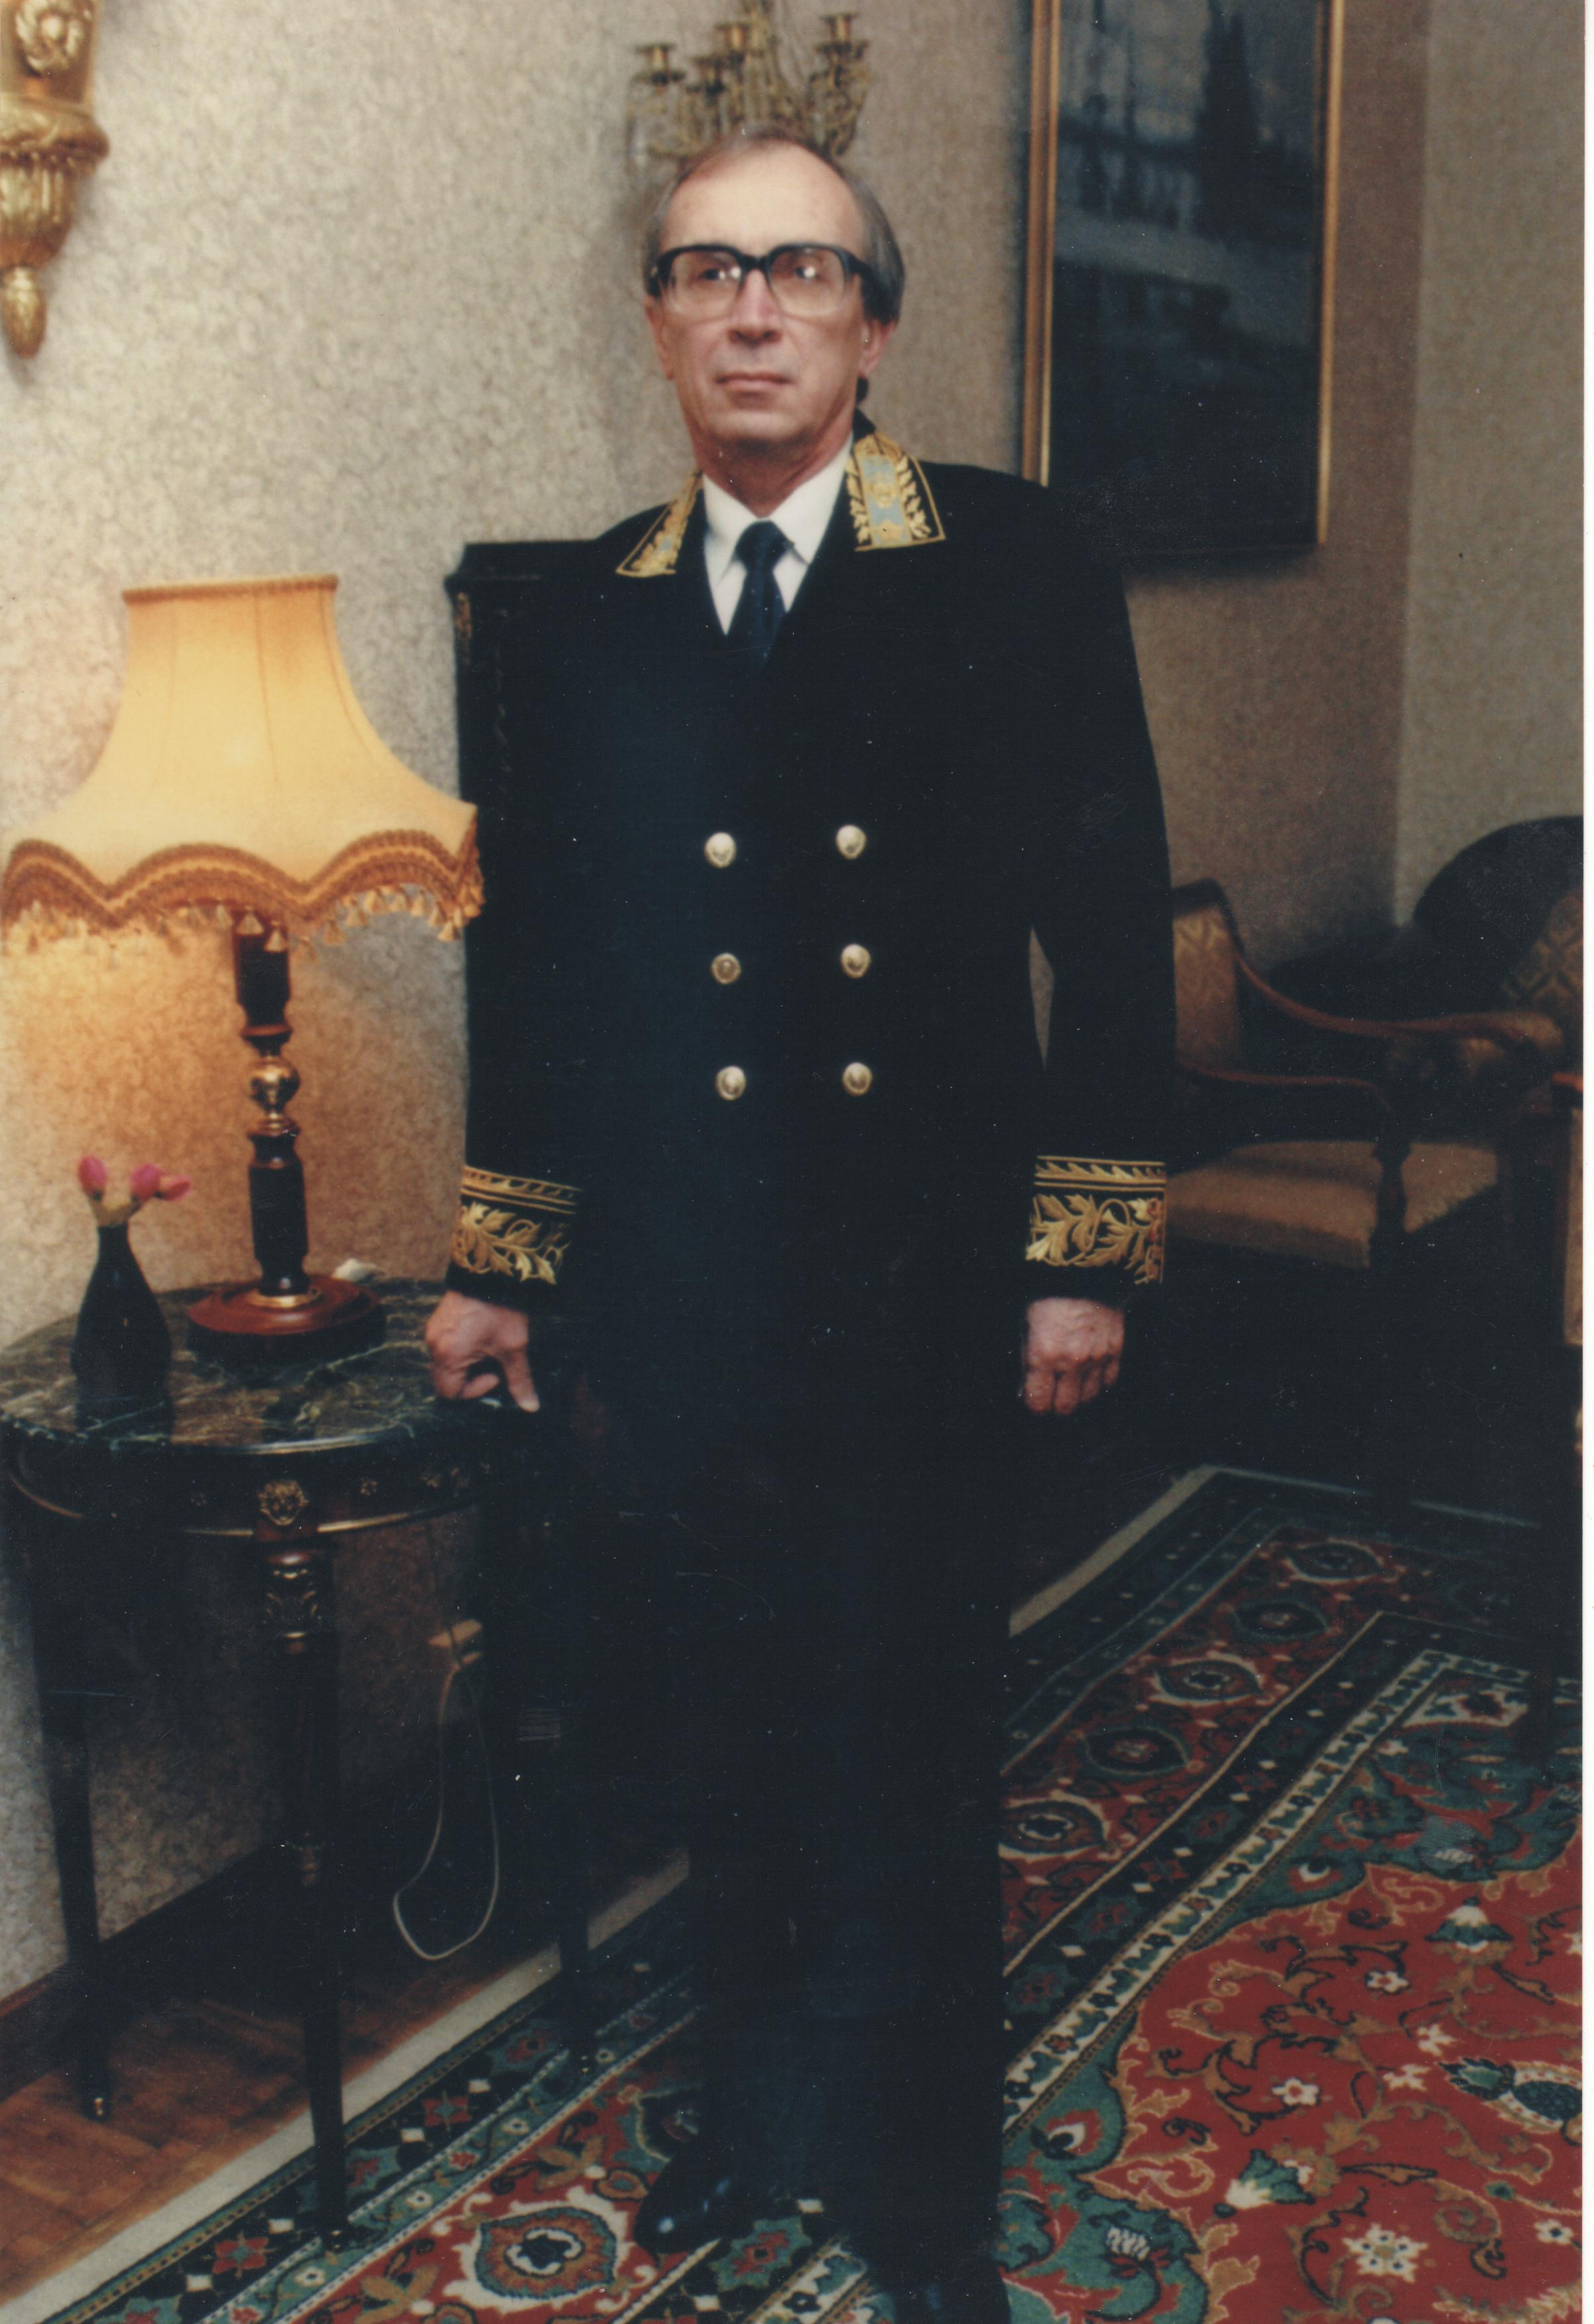
\includegraphics[height=105mm]{inc/77/1}
        \caption{О. А. Гриневский в форме Чрезвычайного и Полномочного Посла.}
\end{figure}

\begin{figure}[ht!]
    \begin{minipage}{100mm}
        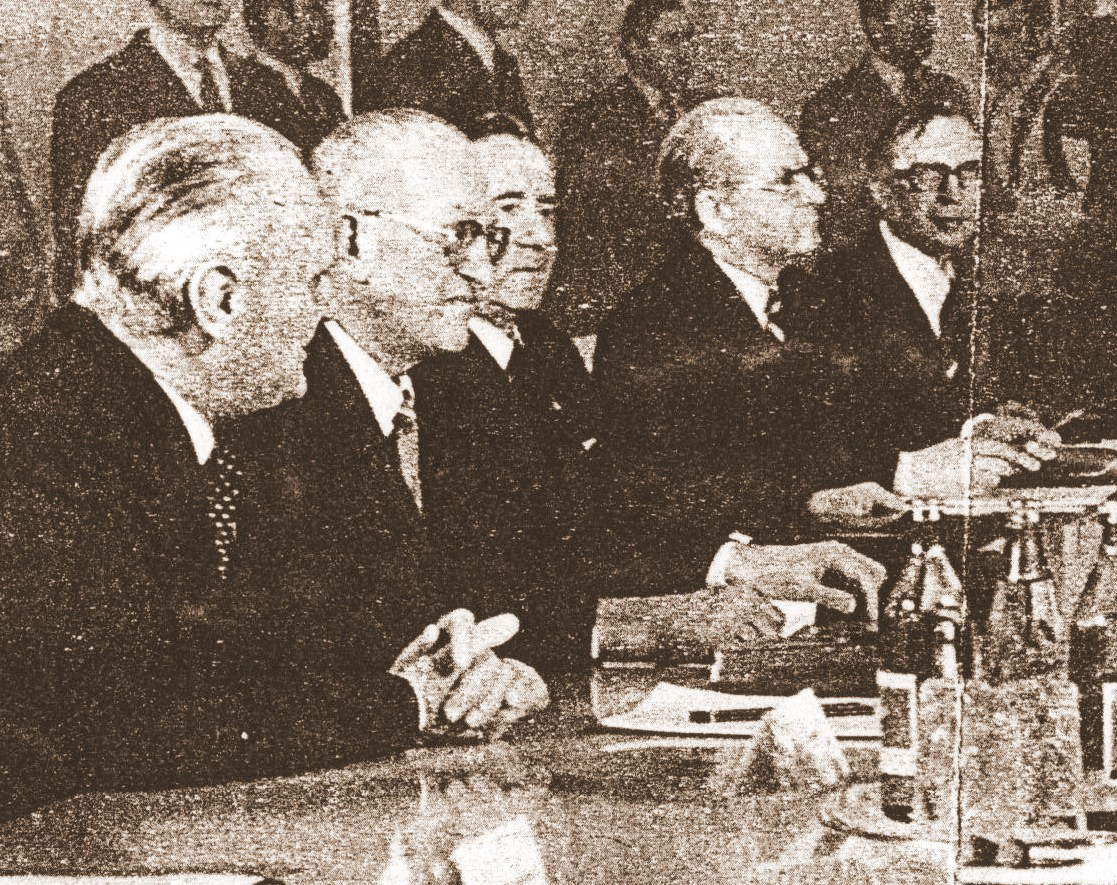
\includegraphics[width=100mm]{inc/77/2}
        \footnotesize{\textit{На международных переговорах. Первый справа~-- О. А. Гриневский.}}
     \end{minipage}
\end{figure}

\vspace{10pt}

\begin{figure}[h!]
\begin{minipage}{100mm}
    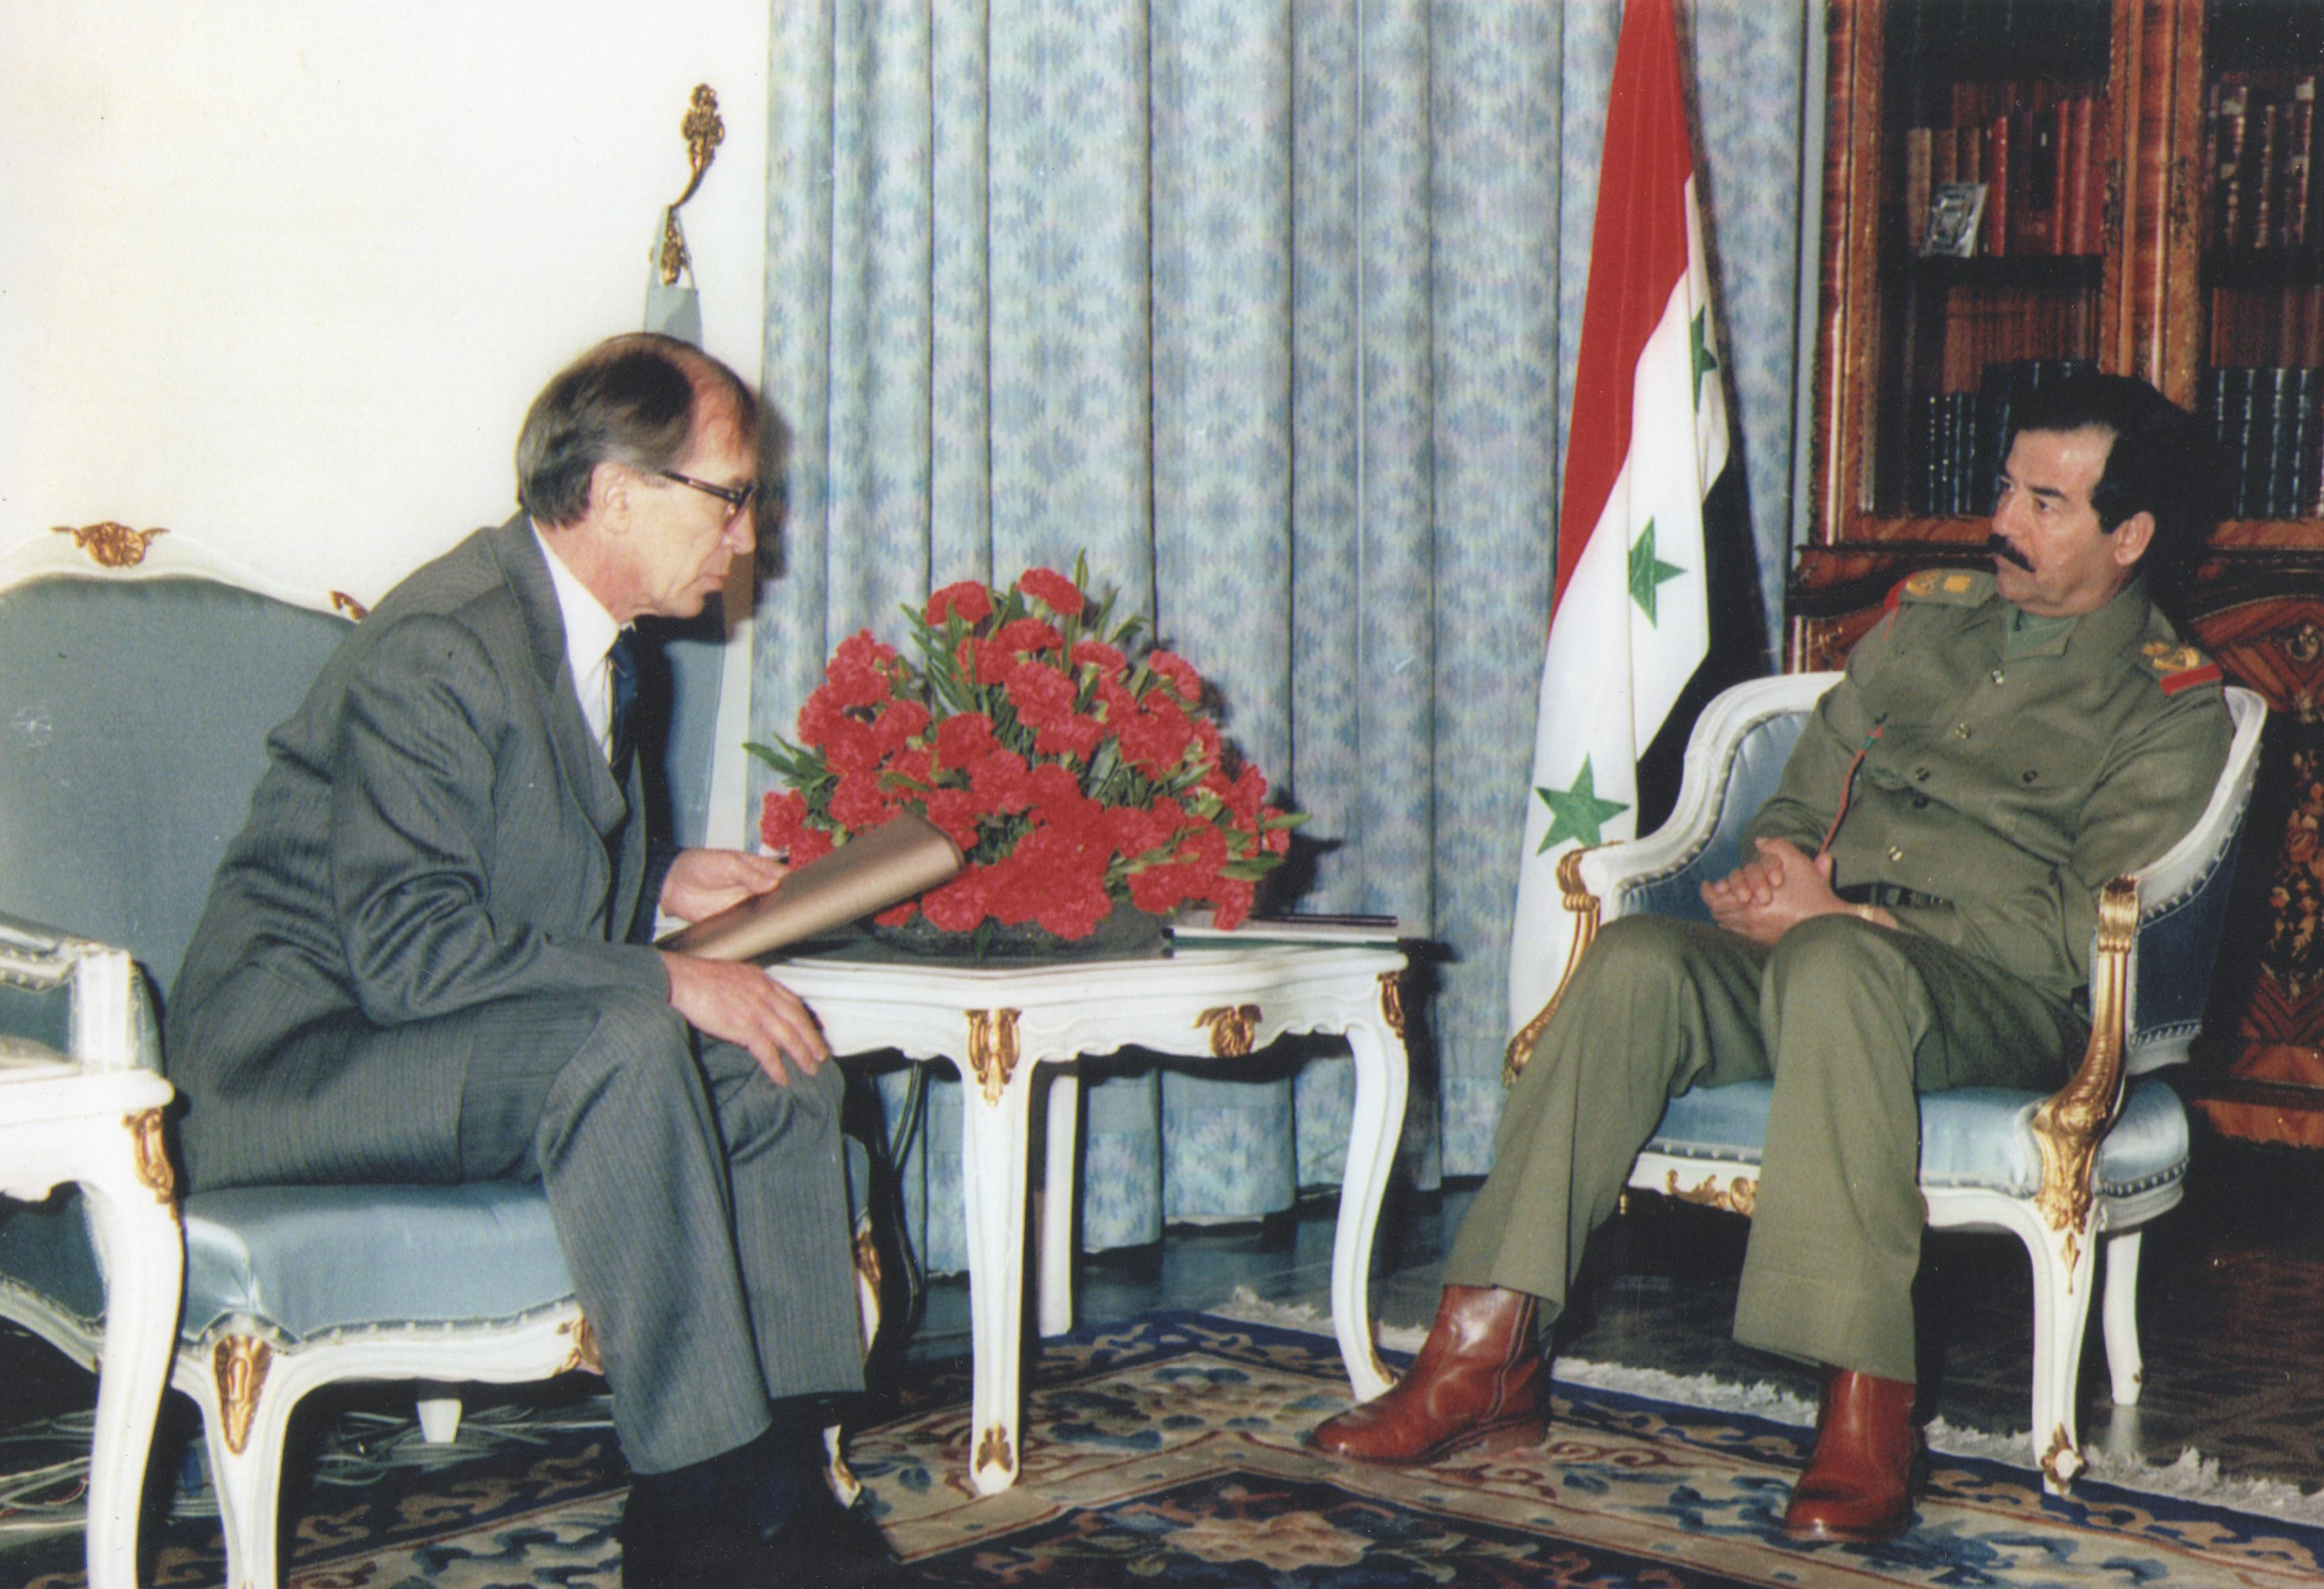
\includegraphics[width=100mm]{inc/77/3}
    \footnotesize{\textit{В духе того времени.}}
\end{minipage}
\end{figure}



\chapter{}
\section*{Из воспоминаний В.Б. Прейса}

Оказалось, что писать прозу мне значительно легче, чем воспоминания.

Во-первых, за много прошедших лет многое выветрилось из памяти и хронология событий сохранилась весьма примерно.

Во-вторых, поскольку дневников я никогда не вёл, то события в памяти восстанавливаются однобоко. Более хорошо вспоминаются взаимоотношения между мальчиками, а девочки остаются в стороне. Поэтому я стараюсь изложить то, что помню, но не исключаю возможных ошибок.

И, в-третьих, до какого времени нужно вспоминать? Мне кажется, что нужно закончить нашим окончанием школы, а всё остальное изложить в эпилоге. По моему мнению, каждый из нас должен написать свои воспоминания, а редактор или редколлегия должны это всё объединить, неважно если будут повторы, тогда может получиться цельная картина.

Итак, я начинаю вспоминать.

\indent

В Москве у Красных ворот, на пересечении Боярского переулка и Хоромного тупика, стоит шестиэтажный дом. Когда то он был серого цвета, а сейчас желтовато-лимонного. Этот дом был одним из первых кооперативных домов, построенных в Москве. В 1929 году он был заселен сотрудниками наркоматов иностранных дел и внешней торговли. В доме проживали ответственные сотрудники аппарата и несколько послов СССР в капстранах. Какое то время в нём жил Нарком иностранных дел М.М. Литвинов.

Дом был семиподьездный, в нём было 93 квартиры. Практически в каждой из них жили семьи с детьми, поэтому при доме функционировал детский сад. В Красном уголке иногда показывали кинофильмы, кроме того при нём работали кружки. Я помню два: автомодельный для старших ребят и драматический для младших.

Мне бы хотелось для полноты картины перечислить детей моего возраста, подростков и некоторых взрослых, которые мне запомнились.

В первом подъезде в квартире № 1 жила семья Яхниных с дочерью Лианой, очень серьёзной девочкой, моей ровесницей. В последствии она стала известным литературным переводчиком.

На втором этаже жили Варзары с сыном Севой и его младшей сестрой~-- Ксеной. Сева был отчаянный парень.
В последствии он воевал, был кавалером многих орденов и медалей, полковником артиллерии в отставке.

В пятой квартире жила семья Гриневских. Их старший сын Олег был нашим приятелем. В последствии он стал Чрезвычайным и полномочным послом, автором нескольких книг.

А в десятой квартире жили Бирюковы с рыженькой дочуркой Лилей и очень интересной мамой~-- Верой Исаевной. Уже будучи взрослым, я очень любил с ней беседовать. А с Лилей мы поддерживаем контакты и сейчас, хотя живем в разных городах США.

В 12 квартире жил Юра Богун. Он был несколько старше нас и был для нас большим авторитетом, он был наш главнокомандующий. Однажды он устроил манёвры. С криками Ура мы бежали на задний двор, а он со своего балкона сбросил на нас большую лампу от прожектора, которая разбилась с таким грохотом, что мы от страха разбежались. После этого его авторитет упал и мы, а вернее, он к нам, потеряли интерес.

На шестом этаже жила семья Меньшиковых. Дочка Таня и её брат Лева были несколько моложе меня. Не знаю почему, но мне доставляло удовольствие пугать их. Они начинали реветь и бежали домой, а вечером их мама Зинаида Борисовна звонила моим родителям и жаловалась на меня.

Во втором подъезде на первом этаже находился детский сад, который я посещал до поступления в школу.
Детский сад я помню весьма смутно. Единственно, что осталось в памяти, так это учительница немецкого азыка. Вернее даже не  она, а стишки, которые мы учили. Некоторые из них я помню и сейчас.

В квартире 23 жила Инна Веселовская, но она была старше нас, и  контактировать с ней мы уже начали после войны.

Двадцать четвертая квартира была многонаселенной. Как я слышал, в ней вначале жил доктор Петров. Когда его арестовали, оставалась жить его дочка. К ней подселился её дядя~-- Петров с женой и сыном Игорем, а потом в третью комнату этой квартиры вселился доктор Штернберг с сыном Шуриком. За достоверность изложенного я не очень ручаюсь, но и Игорь, и Шурик были нашими очень хорошими друзьями. В последствии Игорь стал инженером-электриком, кандидатом технических наук, а Шурик стал врачом-хирургом и женился на Лиле Бирюковой, что было дня меня неожиданностью. К сожалению, его уже с нами нет. Два годя назад он скончался к Америке.

В 26 квартире жила семья Плоткиных. По моему,  он был замначальнимка Правового отдела Наркомата иностранных дел и сгинул, как многие, в 38 году. У него остался сын Миша, но он был несколько моложе нас.

А в 28 квартире жила семья Андреевых, мать и взрослый сын. По-моему, в то довоенное время он уже преподавал в Вузе. К ним периодически приезжал её внук~-- Володя, который после войны долгое время жил у них. В последствии он стал Народным артистом, главным режиссером театра им. Ермоловой.

В третьем подьезде на третьем этаже жила семья Миниксов. Их было два брата, Марик, чуть моложе нас, и Аба, старший. Точного имени его я не знаю. Он погиб во время войны. А напротив жила семья Короткиных, их сын Жора тоже не вернулся с войны.

На третьем этаже в 36 квартире жили Дивильковские. Они приехали в наш дом наверное году в 3б, Их было два брата, Юра~-- старший и Сергей~-- наш ровесник.

Не знаю по какой причине, но до войны мы с ними не общались. Однако, в конце войны и все последующие годы 36 квартира, также как и Красный уголок, были нашим центром времяпрепровождения. Один Господь знает, каких усилий требовалось от Елены Васильевны~-- мамы Сергея, чтобы нас терпеть. В последующем Сергей Иванович Дивильковский работал на ответственных партийных и дипломатических должностях. Во время американо-вьетнамской войны был в Ханое. К сожалению, его старший брат во время войны погиб.

На четвертом этаже жил Миша Гюнтер. До войны мы с ним очень дружили, а потом наши пути как-то разошлись. Он примерно году в пятидесятом умер молодым.

На шестом этаже жили Лёнчнк Кузнецов и девочка Вайола Кофман, приехавшая в 35 году из Америки со своими родителями помогать строить социализм. Насколько я помню, девочка по-русски говорила лишь одно слово ~-- <<робяты>>. Потом она хорошо говорила по-русски, стала кандидатом наук. Сейчас она живет в Америке.

А Лёнчнк Кузнецов был основным моим <<противником>> во время игры в солдатики. В настоящее время Леон Дмитриевич работает в Москве. Он кандидат химических наук.

В четвертом подъезде на втором этаже жила Ирина Каменская~-- <<легендарная>> личность, но о ней несколько позже. Сейчас Ирина Ионовна живет в США. Насколько мне известно, написала комментарий к Библии и котируется в теологических кругах.

На третьем этаже в 47 квартире жили Кунины, приятели моего отца. У них было двое детей~-- Виктор и Ляля. Они были много старше меня.

Заметной личностью в этом подъезде был Штейн. Одно время он был послом в Италии, а позже~-- личным советником Молотова.

Напротив его квартиры жили Рабиновичи. Старший их сын Эмик был военным, а младший~-- Натик, хотя и был немногим старше нас, но с нами не общался. С ним я встретился в 1992 году в Израиле.

Интересным был пятый подъезд. На втором этаже жили Зивы. Их сын Миша подавал большие надежды в музыке. После ареста родителей, его не принимали в консерваторию; требовали, чтобы он отказался от родителей. Консерваторию он всё же окончил и стал довольно известным композитором. В 1980 г мне довелось с ним встретиться. Мы долго вспоминали дом и судьбы его жильцов.

Напротив квартиры Зивов жил Лоренц~-- посол СССР в Латвии. В 1937 г. он и его жена были арестованы и расстреляны. В их квартиру вселилась семья Иванцовых. Со старшим их сыном Сергеем я не дружил, а с младшим Игорем, любил играть. У него были очень красивые игрушки, по-моему японские.

В квартире 59 жила семья Стомоняковых. Он был заместителем Наркома иностранных дел. Как я помню из разговора взрослых, когда его пришли арестовывать, он застрелился у себя в кабинете. Жену расстреляли позже.

На четвётом этаже жила семья Рубининых с двумя сыновьями, Павлом~-- старшим и Андреем чуть помоложе. Они появились а доме перед самой войной. Их отец был послом СССР в Бельгии. В 1950 г. его арестовали как еврейского националиста.

Напротив квартиры Рубининых была квартира Уманских. Они практически всё время жили в США, так как он был послом. У них была дочь Тита. Мы её знали, но видели редко. Где то в конце войны с ней случилась трагедия. Её застрелил сын Министра авиационной промышленности чуть ли не на Красной площади.

Интересной была квартира 66. В ней вначале жил доктор Горелик. По рассказам, которые мне запомнились, он совершил гражданский подвиг. К нему на приём пришёл больной, у которого он заподозрил чуму. Горелик запер кабинет, вызвал спецмашину и она отвезла его и больного в инфекционную больницу, где они и скончались. Когда я уже был врачём, мне пришлось некоторое время работать с его братом С.Л. Гореликом, человеком с трудной судьбой.

После смерти Горелика в этой квартире поселился известный географ, писатель, путешественник~-- Лухманов.
С его внуком Димой до войны я дружил, а затем наши пути разошлись, и я встретился с ним уже будучи взрослым.

Напротив, в квартире 65, жила семья, которая туда вселилась после ареста прежних хозяев. Глава семьи был не то сотрудником НКВД, не то военным. У них был маленький ребенок. С ними же жила сестра жены молодая девушка по имени Маня. Видимо этот военный был очень ревнивый, а может быть был повод к тому, что он застрелил жену и себя. Маленького ребенка забрала бабушка, а Маня продолжала жить в квартире. Наш домуправ, Иван Максимович Калиш, который жил в первом подъезде в подвале, быстро сориентировался и поменялся с Маней. Дальнейшая её судьба была трудной, во время войны она стала доступной женщиной, а где-то к концу войны она поменялась Медниковыми. Их сын Миша стел нашим близким товарищем. В последствии он защитил кандидатсскую диссертацию и стал инженером-атомщиком. Сейчас Михаил Исаакович Медников живет в Израиле.

В шестом подъезде в 71 квартире жили Первины. Во время войны их сын Илья попал в плен, бежал к партизанам, а потом был осужден на десять лет как изменник Родины.

Бывшая квартира Литвинова после его отъезда стала коммунальной и очень несчастливой. Сначала там жил некто Райвид. После его ареста в 37 году туда вселилась семья Досиков, а в 39 году арестовали и Досика. Кроме того, там жила семья Таракановых. С их дочкой Неллей мы дружили.

В квартире 78 до 37 года жили Мельниковы, а после их ареста туда въехала семья Пивень. Он был дипломатом и работал в Чехословакии. В 1939 году его тоже арестовали. У них в семье было две дочери~-- Алла и Мара. Алла была нашей подружкой, мы часто собирались у нее. В конфискованную комнату к ним вселили семью Горностаевых с двумя детьми. Старший Альберт стал нашим приятелем. К сожалению, Аллочка умерла из нашей компании первой, будучи самой младшей из нас.

В седьмом подъезде на втором этаже жили Линские. С их младшим сыном Славой до войны я дружил.

В 81 квартире жили Карские. Он был посол СССР в Эстонии. В 37 году его и жену расстелили. У них осталась одна дочь. А её дочь вышла замуж за Райского Юру, который жил этажом выше.

На третьем этаже жили Райские. У них был внук моложе нас. С его бабушкой после войны мы конфликтовали.

В 83 квартире жили Васильевы~-- тетя и дядя Шурика Штернберга. У них было двое сыновей. Старший Андрей и младший Костя. Шурик нас иногда приводил к ним и мы с удовольствием рассматривали электрическую железную дорогу.

В квартире 85 жили Рафаловские. Квартира была знаменита тем, что когда моя бабушка иногда приезжала к нам, она ходила к Рафаловским молиться. Кроме того, у них жила не то внучка, не то племянница Рита. Она была чуть старше меня, но мы с удовольствием играли друг с другом. А после войны она вдруг стала взрослой дамой и наши контакты прекратились.

В квартире 87 жил молодой военный с женой и трехлетней дочкой. Он был военным атташе, по моему, в Чехословакии. В одну из ночей 38 года их с женой арестовели, а маленькую девочку заперли одну в квартире. Наш дворник~-- Павел Сиротин, всегда бывший понятым при арестах, в эту ночь нашёл брата арестованного и тот забрал девочку к себе. О её дальнейшей судьбе мне ничего не известно.

На 5 этаже в 89 квартире жил бывший царский дипломат Соловьёв с супругой, по национальности немкой. Незадолго до начала войны Соловьёв умер, а в первые месяцы войны была интернирована его жена. Потом в эту квартиру вселили лётчика дальней бомбардировочной авиации. Когда он погиб, его вдова прописала у себя племянника. Я не знаю, что произошло в дальнейшем, но во время войны в квартиру въехала семья Ковалей. Он был начальником московского областного Управления уголовного розыска. У них было двое сыновей. Старший Борис и младший Юрий. С Борисом я учился в одном классе. Он всегда был душой общества и остается таким же по настоящее время. Закончив институт международных отношений, он не пошел по дипломатической линии, а стал учёным. Защитил докторскую диссертацию. Был директором НИИ международного рабочего движения. Сейчас Борис Иосифович Коваль~-- академик. Его младший брат Юра стал известным детским писателем. К великому сожалению, он рано умер. Где-то в конце войны они поменялись с Первиными и переехали в шестой подъезд.

А в 90 квартире жил я с родителями и старшей сестрой Розой. Поскольку она была много старше меня, то мне не возбранялось общаться и с ребятами её возраста, чем я и пользовался. Мое безоблачное детство закончилось в марте 1938 года, когда арестовали маму.

В 92 квартире жила семья Маковских. Они дружили с моим отцом. Сам Маковский был инженер, приехавший со своей женой Шарлоттой Августовной из Германин. Детей у них не было и они по доброму относились ко мне. Мне запомнился запах кофе и до блеска натертый пол. В 1933 или 36 году Маковского арестовали, но быстро освободили и у него, как говорили, была охранная грамота от самого Сталина. Но, несмотря на это, в 1938 году он был вновь арестован и сгинул в неизвестности. Жену же его, также как и Соловьеву, интернировали. Позже мы узнали, что её вывезли в Казахстан. 

Хочу рассказать одни эпизод, оставшийся у меня в памяти. Где-то около четырех часов утра 22 июня 41г. у нас раздался звонок в дверь. В то время этот звонок мог означать многое. Папа открыл дверь. На пороге стояла Шарлотта Августовна. Она отвела папу на кухню, что то ему сказала и ушла. Помню, что папа сказал ей, что этого не может быть. Когда мы его спросили, что случилось, он нам сказал, что Шарлотта слушала речь Гитлера, который сообщил о начале войны с СССР. Папа нас предупредил, чтобы мы никому не говорили об этом, а слушали радио, и днем мы услышали то, о чём говорила Шарлотта.

В 93 квартире жил Рональд Фишзон, он был отчаянным парнем. Году в 1940 он поступил в авиационную спецшколу, но во время войны воевал в пехоте. Был много раз ранен. Вернулся с большим числом наград. Кем он потом работал я не знаю, знаю лишь что под конец жизни он был директором турбазы на Памире.

В конце 1944 или в начале 1945 г. в 22 квартиру, в которой до 1941 г. жил Шейнинг (он был интернирован) вселилась семья Карпухиных. Мария Петровна~-- мама, прекрасная хлебосольная женщина, её сын Толя и дочь Зоя. Она была очень активной девочкой и быстро вошла в наш коллектив, также как и Лиля Бирюкова. В последствии она вышла замуж за нашего товарища~-- Володю Литвинова. Сейчас Зоя Фёдоровна Литвинова прабабушка и пытается воспитывать правнучку.

Ну вот я попытался вспомнить про наш дом и некоторых его жильцов, а теперь вспомним, что мы делали и чем занимались.

Безусловно, события, которые происходили в стране и в мире, мы без внимания оставить не могли. Мы были папанинцами, воевали с фашистами в Испании, летали с Чкаловым через Северный полюс, воевали на Хасане и протягивали руку братской дружбы жителям республик Прибалтики, Западной Украины, Белорусии и Молдавии.

В предвоенные годы мы, как правило, играли в войну. При станции метро <<Красные ворота>> был книжный магазин, в котором мы покупали книжки, имевшие прямое отношение к Красной Армии. Моей любимой книжкой был <<Устав вооружённых сил СССР>>. В 1936 году мне довелось быть с мамой на Первомайском параде на Красной площади. Всё, что я видел, произвело на меня огромное впечатление, особенно прохождение по площади с винтовками наперевес Пролетарской дивизии. Когда я рассказал ребятам об этом, мы пришли к мнению, что сильнее Пролетарской дивизии никого нет и она победит всех врагов. Тревожное положение, которое было в Мире, мы, естественно, не ощущали. Подошло время поступления в школу. Все мои сверстники поступили в школу в нашем районе, а меня записали мои родители в образцовую школу в другом районе, в котором работала моя мама. Мне приходилось туда ездить на трамвае, остановка которого была в конце скверика, где сейчас памятник Лермонтову. Я очень не любил туда ездить и всегда искал причину, чтобы прогулять.

А во дворе в подвалах почему-то начали строить бомбоубежища. Началась финская война. Она мне запомнилась двумя моментами. В моей образцовой школе развернули госпиталь, а нас перевели в далёкую школу да к тому же мы учились в третьей смене. Начинали в четыре и кончали в семь. Это было очень неприятно. Но второй момент был приятным. В том году была очень суровая зима и временами были сильные морозы. В такие дни школа была закрыта, а гулять во дворе нам никто не препятствовал, что мы с удовольствием и делали.

В мае 1941 года Слава Линский, Вайола Кофман, Лиана Яхнина и я закончили пять классов. Начался дачный сезон и многие дети разъехались. А мы в этом году дачу не снимали, так как болела моя тётя и ехать нам было не с кем.

Я прекрасно помню день начала войны. Это был солнечный воскресный день. По улицам, как всегда, ездили машины, трамваи, троллейбусы. Ходили люди. А в двенадцать часов по радио Молотов объявил, что началась война.

Во дворе дома стали собираться группами мужчины. Они были взволнованы, а мы думали, что они волнуются, ведь у нас есть Пролетарская дивизия, самая сильная в Мире.

На другой день наиболее старших из нас собрал дом\-управ и повел всех на чердак. Наша задача заключалась в том, чтобы собрать весь хлам и отнести его к дверям. Взрослые забирали эти вещи и выносили их на улицу. Потом нам дали вёдра не то с известью, не то с мелом и кисти и велели красить деревянные балки. Мы всем этим были очень довольны. А домашние стали наклеивать на стекла крест-накрест бумажные ленты. Нам объяснили, что при взрыве бомбы это может сохранить стёкла.

Папа дома на стену повесил большую карту и чёрными и красными флажками отмечал ход боевых действий. Я удивлялся, Пролетарская дивизия отступала.

В один из дней поступило распоряжение сдать радио-приёмники и фотоаппараты, что мы и сделали.

Большую часть времени я проводил с ребятами на улице. Разнёсся слух, что около метро стоит Каганович. Мы побежали смотреть. Одет он был в форму железнодорожника и что-то говорил окружавшим его мужчинам, а затем с частью из них пошел в НКПС (Народный комиссариат путей сообщения), а мы сопровождали его. В последующие дни мы бегали на Чистые пруды. Часть деревьев там срубили, были вырыты окопы, в которых стояли зенитные пушки и пулемёты, а среди них ходили девушки в военной форме.

В городе была объявлена светомаскировка. Вечером не горели фонари, машины ездили с затемнёнными фарами, а в квартирах окна закрывались чем-либо черным.
По улицам ходили дежурные с противогазами на боку и очень следили за соблюдением светомаскировки. Но было лето, июнь, и на улице было светло.

Я уже не помню какое это было число, но был или глубокий вечер, или ночь, когда завыли сирены. Воздушная тревога. Папа оставался дома, а мы с сестрой пошли в метро, хотя в доме было два бомбоубежища. Очень неприятным был вой сирены, ещё и потому, что мы не знали настоящая это тревога или учебная. В метро почему-то нам пришлось спуститься на рельсы. Было очень грязно и душно. Плакали дети. Никто не знал, что делается наверху. Примерно через час был объявлен отбой и мы узнали, что тревога была учебной.

Мне лично очень досаждала школа, в которой я учился. Оттуда звонили нам домой, приходили и требовали, чтобы меня эвакуировали. Я отчаянно сопротивлялся и пока оставался дома.

Обстановка в городе становилась тревожной. Учреждения, которые располагались в нашем доме, эвакуировались. Сводки с фронтов были плохие. Учебные воздушные тревоги повторялись ещё несколько раз.

Но вот 22 июля, ровно через месяц после начала войны, ночью вновь завыли сирены. Мы подумали, что это опять учебная тревога. Но не успел ещё диктор закончить фразу: <<Граждане, воздушная тревога>> как послышались пулеметные выстрелы, а небо располосовали лучи прожекторов. Мы быстро побежали в бомбоубежище. После отбоя я со старшими ребятами пошел на Чистые пруды. Там девушки возились около пулеметов. На наши вопросы они не отвечали и велели идти домой. Кто-то сказал, что в районе вокзалов есть разрушения и взрослые ребята пошли туда, а я вернулся домой. Дома папа, он тоже был очень возбужден, рассказывал, что они действительно видели с крыши пламя в районе вокзалов, но наиболее сильные пожары были где-то в районе Серпуховки.

На следующую ночь или через ночь, я точно не помню, вновь была объявлена тревога. Я упросил папу, чтобы он взял меня на чердак. Там я встал под балкой у слухового окна. Стрельба и взрывы были довольно сильные. Было впечатление, что горит весь город. Взрослые говорили, что это горит лакокрасочный завод на Пресне. На крышу сыпалось большое количество осколков, некоторые из них пробивали железо и падали на чердак. Мужчины стояли под балками и прикрывали головы лопатами. Папа велел мне спуститься в убежище, вход в которое был около нашего подъезда. Я вышел во двор и перебежал в свой подъезд. Мне не хотелось спускаться в убежище и я остался стоять у дверей. Но в это время раздался такой силы взрыв, что мне показалось, будто дом подпрыгнул. Меня отбросило к одной стене, потом к другой и ... я не помню, как оказался в убежище. Меня спросили, что произошло снаружи и я ответил, что где-то близко от нас что-то взорвалось. После отбоя, дома папа сказал, что был очень сильный налёт, в городе много пожаров и где-то недалеко от нас взорвалась крупная бомба. Уже будучи юношей, из книги В. Лациса <<Буря>> я узнал, что по наводке немецкий лётчик сбросил бомбу большой мощности на здание Представительства Латвии, где в это время находилось всё Правительство республики. Это было на улице Чаплыгина, действительно довольно близко от нас.

Двор постепенно пустел, детей, практически, никого не осталось. И вот пятого августа бабушка, тетя, двоюродный брат и я отправились в эвакуацию. Уезжать мне не хотелось, но постоянные водушные тревоги и днём, и ночью, сделали своё дело.

Первый день нашего отъезда, а ехали мы в теплушках, ознаменовался неприятным эпизодом. К вечеру мы прибыли в Рязань. Наш эшелон остановился между воинским эшелоном, идущим на запад, и санитарным поездом, идущим на восток. Мы впервые увидели раненых. Вдруг раздался сигнал воздушной тревоги, а через некоторое время начали стрелять зенитки. Оба эшелона ушли по своим направлениям, а мы остались. У меня появилось такое чувство, что нас бросили. Через некоторое время всё закончилось и я успокоился. Последующий наш путь проходил без происшествий, если не считать, что я чуть не отстал от эшелона в Куйбышеве.

На пятые сутки мы прибыли на станцию Раевская Башкирской АССР. Эшелон разгрузили. Куда нас повезут дальше никто не знал. Кругом стояло много подвод. Нас посадили на одну из них и сказали, что мы едем в деревню Райны. Это недалеко~-- 60 км. Где-то ближе к вечеру нас и ещё четыре семьи привезли в эту деревню. Меня поразило, что крыши всех домов покрыты соломой, а не железом. К нашей подводе подошел мужчина и сказал чтобы мы ехали за ним. Вскоре мы подъехали к дому, из которого вышла молодая женщина и стала что-то говорить на непонятном языке. По её жестам мы поняли, что здесь мы будем жить. Дом был большой, но и семья у этой женщины была большая и конечно было тесно.

Через некоторое время мы с тётей нашли другой дом, где практически были одни. Его хозяйка, пожилая женщина Фатима-оби, жила на хуторе и приходила в дом редко. Единственная сложность для нас заключалась в том, что заготавливать дрова мы должны были сами. В отличие от других домов деревни, крыша у нашего дома была драночная, а не соломенная и, кроме того, он был огорожен деревянным забором, а не плетнём. Со стороны улицы у забора лежал большой камень, на котором мы любили сидеть. Хочу сделать небольшое отступление. В 1971 году, т.е. через тридцать лет после эвакуации, мне довелось посетить эту деревню. Деревня всегда была очень большой, а сейчас это стал просто агрогород. Большинство домов уже имело железные крыши, имелось электричество и радио, чего раньше не было. Единственно, что осталось неизменным, это непролазная грязь на улице. Так вот, я стал искать дом, в котором мы жили. Дома не было. Оказыватся он сгорел, но я узнал камень. Какой же он оказался маленький.

Единственным работником на первых порах был я. Это дало мне возможность научиться запрягать лошадь, косить траву, работать на сенокосилке, копать картофель, воровать на бахче арбузы, а на поле подсолнухи, но это было всё несколько позже.

В мои обязанности по дому входила доставка воды и я научился носить вёдра на коромысле, пилка и рубка дров, а также растапливание печи. Поначалу не всё получалось, но потом я освоился. Нам сказали, что Правление колхоза выдает эвакуированным муку. Нашей семье полагалось 20 килограмм, и за ней нужно было идти на другой конец деревни на склад. Сколько это 20 кг, ни мои родичи, ни тем более я, не представляли. Надо отметить, что я был довольно слабеньким, не высокого роста, мальчиком. Мне дома дали наволочку и я отправился за мукой. Я уже говорил выше, что грязь на улице была непролазной, и ходить по этой дороге было сложно даже без груза. На складе мне взвесили муку и помогли взвалить наволочку на плечи. Пошатываясь я вышел на улицу и через пару шагов мешок у меня свалился. Поднять его я не мог, а только переставлял шага на два. Я не знал, что мне делать, но ко мне подошла женщина и стала что-то говорить мне по татарски. Язык я, естественно, не знал, но понял, что она велит мне оставаться на месте и никуда не уходить. Она ушла и скоро вернулась с тележкой, помогла мне положить на неё наволочку с мукой и мы поехали. Через какое то время она показала мне дом. Я понял, что она здесь живет и сюда нужно вернуть тележку, что я и сделал. После этого я понял, что такое 20 кг. Я не буду описывать как мы жили в эвакуации~-- это тема отдельного повествования, скажу лишь одно, основной нашей пищей была картошка. Однажды с ребятами я охотился на голубей и нескольких принёс домой. В этот день мы ели голубиный суп.

В конце октября 1941 г. к нам приехали из Москвы папа, сестра и папин брат. Мужчины пошли работать и жить нам стало полегче.

В начале 1942 г. к нам из госпиталя приехал папин младший брат. У него была тяжелейшая контузия и он долго лежал в Свердловске в госпитале. В конечном счёте он был признан негодным к службе в армии. По состоянию здоровья в колхозе он тоже работать не мог. Через некоторое время они с папой решили вернуться в Москву, но папу не пропустили и он возвратился к нам. Где-то в апреле 1943 г. Папа съездил в Уфу и ему удалось устроиться там на работу. Он вернулся за мной и пятого мая, эту дату я очень хорошо запомнил, мы приехали в Уфу. У папы уже были продовольственные карточки и около вокзала мы их <<отоварили>> как тогда говорили, купив пять килограмм хлеба. Пока мы дошли от вокзала до дома, где нам предстояло жить, хлеба у нас уже не было.

Я уже упоминал, что перед войной я закончил пять классов. В деревне я не учился, так как там была только четырехлетка, да и та на татарском языке, поэтому я пропустил два года. В Уфе я пошел учиться в шестой класс. От школы я отвык и мне было несколько трудновато, однако учился я неплохо.

В январе мы получили пропуск и вернулись в Москву. Мы приехали как раз в период школьных каникул, меня записали в 310 школу и десятого января я пошёл учиться. Школа была только для мальчиков, сколько нас было в классе я не помню. Первый день ознаменовался для меня двумя событиями. Мы писали диктант и к моему удивлению и ужасу я сделал тринадцать ошибок, причём одна была нелепее другой. Из всех ребят в классе мне запомнился один. Он был очень активный, гонялся за кем-то по классу и в конце концов с учительского стола сбросил чернильницу на пол, которая, естественно, разбилась. Пришла учительница, вызвала директора по кличке <<Бегемот>> (он был очень толстый). Естественно первым вопросом был : <<кто это сделал?>> Ответа не последовало. Тогда директор сказал: <<Будете сидеть до тех пор, пока не сознаетесь. Принесите им ведро,~-- сказал он нянечке,~-- и заприте дверь класса>>. Всё было выполнено. Сознаваться никто не собирался и все были рады, что занятий не будет. А с мальчиком, который разбил чернильницу, я подружился, его звали Володя Литвинов.

Стало темнеть, мы зажгли свет в классе и потянулись к ведру. Стали появляться родители. Наконец пришли и за мной, а за Володей никто не приходил. Позже я узнал, что через некоторое время всех оставшихся директор отпустил.

А во дворе было уже много ребят и мы практически все учились в одной школе. И девочки тоже учились все вместе. Среди мальчиков появился новенький~-- Боря Коваль и присоединился Серёжа Дивильковскмй.

Мне запомнился один эпизод, относящийся к этому времени. В начале июня 1944 г. по Москве должны были провести пленных немцев. Как назло, в этот день утром у нас был экзамен по алгебре. Но мне было не до алгебры, мне очень хотелось посмотреть на немцев. Экзамен был устным и что я там наболтал, не помню. Но получив оценку, тут же побежал на Садовое кольцо. Немцев я не пропустил.

Нашим ребячьим увлечением в это время был футбол. Рядом с нашим домом находилась довольно приличная площадка, которую по чьей-то хорошей идее назвали Папанин-бридж. Причин для названия было две. Говорили, что в доме, где была эта площадка, жил Папанин, а слово бридж было присвоено потому, что команда московского <<Динамо>> совершила триумфальное турне по Англии. Так вот этот Папанин-бридж на многие годы стал для нас центром притяжения. Кроме того, мы выезжали играть в футбол и за город. Чаще всего в Болшево. Противниками нашими были ребята из соседнего дома, У них было два очень сильных игрока~-- Володя Епишин и Коля Фролов. Кто был ещё в их команде я не помню, но честно признаюсь~-- они играли лучше нас. И мне как вратарю это было особенно известно.

С девочками у нас в это время особых контактов не было.

Я уже упоминал, что в доме был Красный уголок. Практически каждый вечер мы там собирались, играли в биллиард или просто дурачились. Но мы становились старше. Появился патефон, стали приходить девочки. Я притащил из дома флирт и началась переписка. Почему-то на память приходит такая сентенция:

<<Лютик: Маргаритка, вы мне нравитесь! И следует ответ: Все мужчины крокодилы!>> А чуть позже мы уже стали собираться у Аллочки Пивень или у Люции Фроловой дома. Традиционной едой был винегрет. Не обходилось и без выпивки. Любимое вино~-- три семерки.

Следует отметить, что мы жили достаточно вольной жизнью. Родителям было как то не до нас. Но мне хотелось бы подчеркнуть, что ничего предосудительного мы
себе не позволяли.

Кому первому в голову пришла мысль об объединении всех нас, проживающих в разных домах в <<Союз>>, я не помню. Мне кажется, что Игорю Петрову, но как бы то ни было, в 1947 году был создан Союз Соединенных Домов~-- ССД. Тайным голосованием (по моему голосовали одни мальчики) был избран Президент~-- Сергей Иванович Дивильковский, Председатель Совета Министров, он же Министр финансов~-- Олег Алексеевич Гриневский и Министры: Министр Вооружённых сил~-- Борис Иосифович Коваль, Министр внутренних дел~-- Александр Александрович Штернберг, Прокурор~-- Владимир Матвеевич Литвинов, Министр Кинематографии, он же редактор журнала <<Вундеркинд>>~-- Виктор Борисович Прейс. Кроме того, у нас был свой собственный Патриарх и по совместительству Муллейшнй, Буддейший и Раввинейший~-- Игорь Михайлович Петров. Все остальные были граждане ССД, только лишь Зоя Фёдоровна Карпухина присвоила себе звание женделегатки от второго подъезда.

Одновременно с образованием ССД стал выходить журнал <<Вундеркинд>>. Когда я сейчас просматриваю его меня поражают две вещи. Во-первых, жуткое количество грамматических ошибок (а ведь я был его редактором под фамилией Кебзак, и, во-вторых, то, что мы там писали, по тем временам тянуло на 58 статью УПК. И хотя прямой антисоветчины не было, но многие вещи преподносились как пародия, как насмешка над действительностью. Однако мы, в силу своей дурости, над этим не задумывались.

Итак, в 1947 году было создано Государство, объединившее значительное число мальчиков и девочек со всей округи. Например, Томочка Зайцева жила на Чистых Прудах, а Миша Стояновский на Сретенке.

Как и положено Государству, мы имели свой Гимн. Автором его был Игорь Петров, а музыка была взята из модного тогда кинофильма <<Девушка моей мечты>>. Ниже я привожу слова Гимна:

\indent

{\itshape

Славься, славься государство наше.

Самая прекрасная Страна,

Ты всех стран сильней, могуче, краше.

Круглый год в тебе стоит весна.

\indent

Славься, славься ССД вовеки.

Демократия в тебе сильна! 

Здесь живут свободно человеки! 

Круглый год в тебе стоит весна.

\indent

В ССД вся власть в руках народа.

Много в нём закусок н вина.

В ССД господствует свобода!

В ССД всегда стоит весна!
}

\indent

Конечно, то, что писалось в журнале, было очень наивным. Но журнал ждали и читали с удовольствием. С моей точки зрения, были и хорошие стихи и рассказы. Одним из таких стихотворений было стихотворение, написанное Сергеем Дивильковским под псевдонимом С. Тютюн-Брджиевскнй. Я привожу его с некоторым сокращением. Называлось оно <<Московские рынки>>.

\indent

{\itshape

Трубная площадь. Центральный базар,

Скверик, трамваи, милиция.

Шум деловой. Цветной бульвар.

Вопли обманутых. Жизнь многолицая.



Был я в Берлине, гулял по аллее 

Unter den Linden~-- красиво! Картинка!

Но об одном я серьезно жалею.

Нету в Берлине хорошего рынка.



Наш бы московский немецкий рынок 

Взять бы, да к немцам в логово.

Да, а то что это? Как ботинок 

Для человека безногого.




Эх, вот Москва! Исторический запах. 

Преображенка. Дух истории.

Будто в Петровых огромных лапах 

Две столицы из-за рынка спорили.

Стой и любуйся! Год ли, час ли,

Минуту стой или две.

Как вы, не знаю, а я лично счастлив,

Что проживаю в Москве!
}

\indent

Журнал мы издавали ровно год, а потом вынуждены были прекратить. Причина тому была следующая. Двенадцатый номер журнала мы принесли в школу на вечер и там его либо потеряли, либо его кто-то специально передал директору. В разгар вечера меня вызвали к нему в кабинет. Там сидело довольно много учителей. Меня спросили, наш ли это журнал. Я ответил утвердительно, поскольку там были наши имена и фамилии. Должен сделать небольшое отступление. Учился я слабо, моими основными оценками были тройки. Директор мне сказал:

Виктор! Лучше потрать твои мысли и фантазию на учебу, а не на журнал.

Конечно этот разговор был мне неприятен, тем более, что моя биография была подмоченной. После этого выпуск журнала прекратился.

Однако у Олега Гриневского есть другая версия, будто пионервожатая из школы Аня Кулагина вызвала его и сказала, что надо кончать это дело, иначе могут быть большие неприятности. Он нам сказал об этом и мы перестали выпускать журнал. Я лично такого факта не помню.

Пережили мы и ещё один неприятный момент. Но Все по порядку. Наш очередной домуправ~-- Александра Никитична со своей дочкой жила в Красном уголке. Она не очень препятствовала нам, когда мы там находились. В томже Красном уголке на тумбе стоял бюст Сталина. В один из вечеров мы уж очень расшумелись и разбегались и кто-то зацепил эту тумбу, она закачалась. Мы остолбенели. Вдруг бюст вождя, а он был гипсовый и покрашен под бронзу, упал на пол и с жутким грохотом разбился. Из своей комнаты выскочила Александра Никитична, увидела это дело и полушёпотом нам сказала:

\textit{Всё на задний двор и в пыль.}

Мы выполнили её распоряжение и всё, что было ранее Вождём, превратили в пыль.

Но не всегда наши отношения с Александрой Никитичной были ровными. Иногда мы ей надоедали и она выгоняла нас, запирая изнутри дверь. В один из таких эпизодов, она нас всех выгнала, но Камека (Ира Каменская) спряталась, через некоторое время открыла нам дверь и мы снова захватили Красный уголок. По этому поводу Сергей написал балладу: <<О взятии Красного уголка>>. Кроме всего, там были такие слова:

\indent

{\itshape
А главная осады героиня, храбрее не сыскать нам человека, зволась она де Лякруа ~-- графиня, а попросту, по нашему, Камека!
}

\indent

Так вот о Камеке. Настало такое время, когда мы стали обращать внимание на девочек, а они на нас. Меня любила Люция, Шурик любил Ксену, а Боря Таню Меньшикову. Но наши отношения были очень чистыми. А Камека страстно любила Володю Литвинова. Но это не мешало ей утверждать, что она никогда не поцелуется с мальчиком. Но к нашему изумлению (девочкам наверное это было известно) первая вышла замуж. Но самое примечательное в другом. На утро после первой брачной ночи, она в красивом, по моему в голубоватом, платье, выбежала во двор, стала бегать и кричать <<Я женщина, я женщина !>> Это было очень забавно.

Уже здесь, в Америке, я связался с ней и предложил тоже написать свои воспоминания, но она отказалась, ссылаясь на занятость. Но в то же время рассказала мне, что когда она вышла замуж и в дневное время занималась с Сеней любовью, со двора неслись крики: <<Зоя - штандер, Игорь - штандер>>, но это их не отвлекало.

А потом мы закончили школу, практически все поступили в институты и на этом наше отрочество закончилось.
Какое то время ССД существовал лишь номинально. Иногда небольшими группами мы собирались, но массовых сборов не было.

А через 40 лет мы собрали весь ССД. В гостинице <<Интурист>> был устроен банкет и выпущен юбилейный номер Вундеркинда. После этого вечера периодически мы стали собираться, чаще всего у Люции. Это были приятные вечера.

А жизнь шла своим чередом. Уехали в Америку Камека, Лиля с Шуриком и я с Галей. Миша Медников уехал в Израиль

К сожалению, появились у нас и потери. Первой ушла от нас самая молодая~-- Аллочка Пивень, потом Воля Голубев и Миша Стояновский, а недавно и Шурик Штернберг~-- светлая им всем память.




\chapter{}

\section*{Из воспоминаний М.В. Миникса}

\textbf{О хозяйстве и работниках Дома у Красных ворот\protect\footnote{Пишу все, что вспомнил и как помню. Другие могут рассказать о том же, но по-своему. Мне кажется, это (такие повторы)~-- не страшно.} (<<дома образцового содержания>>).} Нашим замечательным Управдомом долгие годы был Иван Максимович Калиш. Сохранилась фотография, на которой изображена скамейка в садике нашего Дома, а на ней мы с папой, Иван Максимович и А.И. Кузнецов. Подобные фотографии есть и в других семьях, поскольку И.М. Калиш со многими жильцами дома был в приятельских и даже дружеских отношениях. Потом его место заняла Александра Никитична Давыдова, которая уже в 50-е годы поселилась в 6-ом подъезде нашего Дома.

Все аварийные ситуации в Доме успешно побеждали свой мастер на все руки (слесарь-сантехник, электрик и проч.) N.N. Барский и его помощница Наташа. Если не ошибаюсь, в конце сороковых годов дочь Барского вышла замуж за старшего сына полковника Иванцова из 5-го подъезда. Был и свой столяр, который с семьей жил в подвале 5-го подъезда (за Красным уголком).

Весьма авторитетной фигурой для нас, мальчишек Дома, был Главный дворник Дядя Павел. А был еще второй дворник N. Шапиро.

В Доме была оборудована собственная котельная для обогрева квартир зимой, а в ванных вода нагревалась с помощью газовой горелки фирмы <<Юнкерс>>, что казалось забавным для детей войны. Некоторые жильцы у себя в квартирах сделали отвод горячей воды из ванной на кухню (по тем временам~-- чудеса да и только!). Кто был Главным истопником~-- не помню, но у него было два сына: Ислам и  Мареф. Вход в котельную был с заднего двора, а окна из нее выходили в подвал под вторым подъездом. Как-то летом, уже в конце 50-х или в начале 60-х, из этого подвала появилась перепачканная мордашка очаровательной девицы лет трех, которая доверительно обратилась ко мне с жалобой на жизнь: <<Я один, совсем один... мне так грустно...>> (детей во дворе~-- никого; это была дочка одной из сестер Гущиных, которая вышла замуж в Румынии и гостила у родных).

В Доме работали лифты (в 30-х годах это было событием). Вначале лифтеры круглосуточно дежурили в каждом подъезде. Затем, по два лифтера обслуживали все лифты. Их штаб-квартира располагалась в сторожке, а она~-- в подворотне.

Внутридомный Детсад (подробнее см. выше~-- воспоминания О.А. Гриневского) вначале размещался во 2-м подъезде, а затем  расширился за счет места для квартир первого этажа 3-го (окна на улицу) и 4-го (окна во двор) подъездов. Для ребят всех возрастов организовывались экскурсии по Москве.

В Доме еще до войны работал стол продовольственных заказов. Для постоянных клиентов в стену подворотни был встроен блок из двадцати с лишним сейфов-ячеек, в которые загружали готовые заказы, а каждый из клиентов имел ключ от своей ячейки. Привозили заказы на открытом пикапе. Мы помогали его разгружать; за это нас катали по двору (по улице нельзя!).

Пункт приема в стирку и выдачи чистого белья был организован в подвале 1-го подъезда, а затем перекочевал в подвал под 7-ым подъездом. В этом подвале в разные времена работала столовая (был и буфет).

Собственная снеготаялка располагалась около ворот заднего двора, недалеко от котельной. Мусоросборник и мусоросжигалка также была на заднем дворе (около окон 3-го подъезда).

Особое место занимал и особую роль в жизни Дома играл Красный уголок, расположенный в подвале 5-го подъезда. В нем занимались самыми разнообразными делами и развлекались:

\begin{itemize}
\item проводились собрания жильцов, занятия Ликбеза, выступали агитаторы в период проведения первых послевоенных выборов, готовились стенгазеты;
\item работали различные кружки: радиолюбителей, хоровой, драматический, моего сына учили даже играть на фортепиано, правда, не очень успешно;
\item иногда <<крутили>> кино, проходили концерты художественной самодеятельности;
\item работала библиотека;
\item можно было поиграть в бильярд, в настольные игры;
\item и многое-многое другое.
\end{itemize}

Это все были замечательные особенности Дома у Красных ворот.

Были и свои казусы:
\begin{itemize}
\item маленькие, в некоторых квартирах~-- крохотные уборные;
\item кухни трех размеров: крохотные, небольшие и побольше (до 8-9 метров);
\item во многих квартирах были предусмотрены шкафы-холодильники (с окошком на улицу), во многих~-- нет;
\item в одних квартирах были балконы, в других~-- нет, например на 3-м этаже 3-го подъезда: в кв. 35 был огромный балкон, а в кв. 34 и 36 балконов не было;
\item в <<левых>> (при подъеме по лестнице~-- налево) квартирах 3-го подъезда были затемненные комнаты и кухни (виноват странный выступ~-- квартиры 2-го подъезда). 
\end{itemize}

Я уже не говорю о том, как Дом образцового содержания пострадал за свои привилегии, сколько людей~-- не только Наркоминдельцев~-- погибло в сталинских застенках.

\textbf{Хорошие люди (из книжки <<О людях дома у Красных ворот>>).}Хороших людей в нашем доме было, конечно, больше, чем упомянуто в этих воспоминаниях. Запомнилось то, что забыть нельзя, да и не хочется.

Нашими ближайшими соседями были Кузнецовы: Алексей Ильич, Варвара Николаевна, ее дочь от первого брака Александра Гавриловна и внучка Ия Бабенко, одноклассница моего брата Абы (1924 г.р.). Самой близкой была баба Варя, добрейший человек, истинная христианка. На Пасху она угощала нас куличом, а во время войны~-- блинчиками из картофельных очисток. Она почему-то любила сажать меня на стол, лет до пяти. До сих пор чувствую ее теплоту.

Рядом с ними жили Е. В. Голубева~-- мудрая, очень выдержанная, интеллигентная женщина, и ее сыновья: Юра (погиб на войне) и Сережа (см. раздел VIP) Дивильковские. Как дорогую реликвию храню книгу «Славные большевички», которую с теплой надписью подарила моей маме Елена Васильевна. В этой книге она написала о своей маме, Марии Петровне Голубевой (Ясневой), члене партии с 1901 года, которая всю жизнь была честным и бескорыстным работником. Ее хорошо знал и ценил В. И. Ленин, тепло принимали члены его большой и дружной семьи (в начале века).

На шестом этаже, над нами, жили Дмитрий Афанасьевич Кузнецов~-- профессор, доктор, проректор Менделеевки, его жена Мария Леоновна~-- доцент того же института, их дети Галя (Ая) и Леончик.



В тяжелые послевоенные годы, когда мы с мамой жили впроголодь, и о покупке чего-либо из вещей не могло быть  и  речи,  Мария Леоновна или Леончик периодически приносили мне то рубашку, то костюм, то свитер. Все вычищенное, выглаженное и аккуратно сложенное. Однажды кто-то из них принес толщенное, тяжеленное пальто.

Через несколько дней к нам спустился Дмитрий Афанасьевич. В руках у него было шикарное, на мой взгляд, зимнее пальто с каракулевым воротником. И вот этот большой ученый и большой человек со смущенным видом стал объяснять мне, паршивому мальчишке (а был я, действительно, не сахар), что домочадцы случайно отдали важную для охоты (или рыбалки?) одежку и что он извиняется передо мной (!, что просит меня (!) принять, вместо того~-- это, правда~-- хорошее, пальто.

\newgeometry{left=0mm, right=0mm, top=0mm, bottom=0mm}

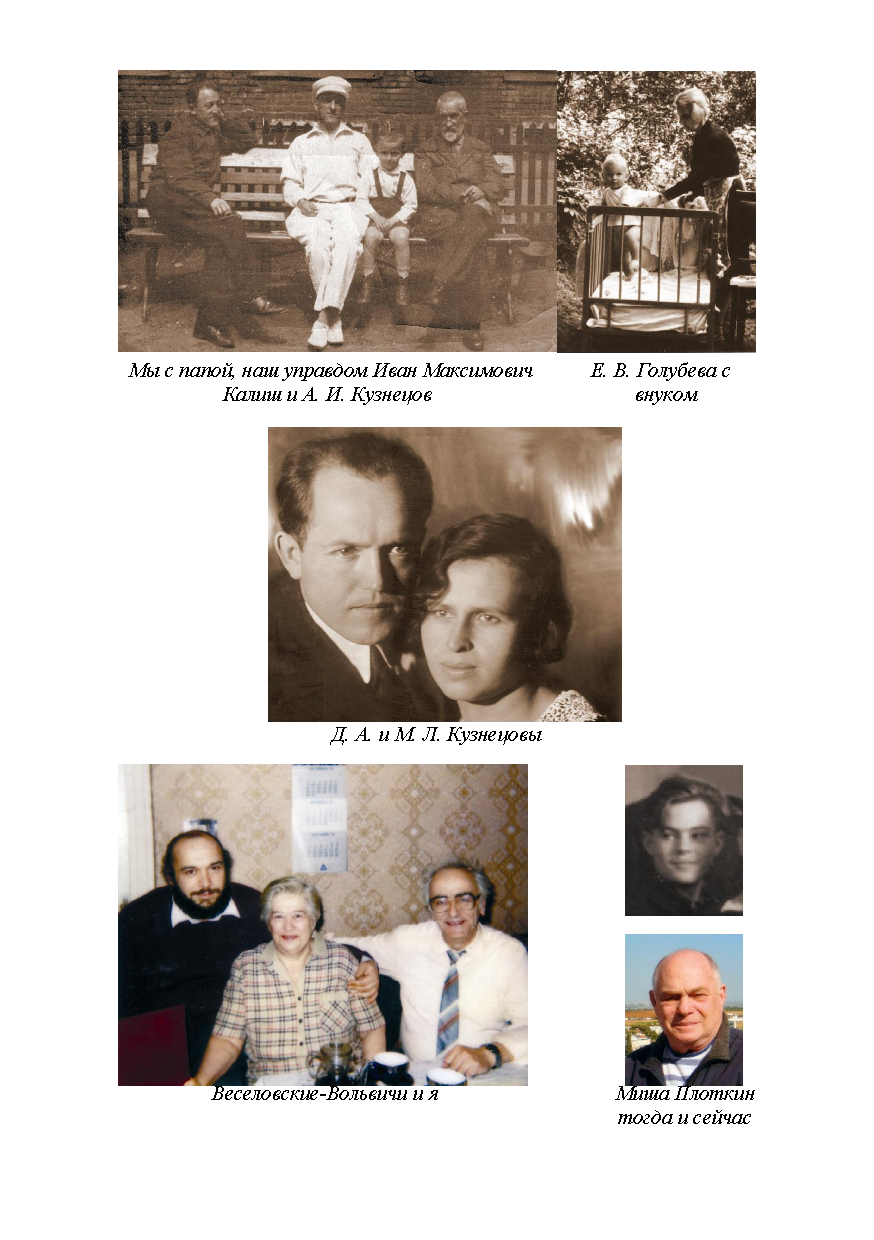
\includepdf[pages=-]{inc/fragment.pdf}

\restoregeometry

Такое невообразимое поведение на всю жизнь осталось для меня уроком такта и благородства.

В нашем же подъезде, на пятом этаже, жили Александровские: Андрей Сергеевич, Мария Осиповна и Лёлька~-- моя сверстница (о ней~-- отдельно). Родители Лёльки были высокообразованными людьми с широким кругом интересов. В доме у них была какая-то особая атмосфера. Там никому не пришло бы в голову громко разговаривать или ругаться. В этом доме я впервые услышал качественные записи музыкальной классики в превосходном, по тем временам, воспроизведении, увидел хорошие репродукции великих картин. Видимо, есть доля вины этих людей в том, что через несколько лет я стал «гурманом» в соответствующих областях культуры.

Ирина Сергеевна Веселовская из второго подъезда относилась к промежуточному поколению (1926 или 1927 г. р.): между «старшими ребятами» и сверстниками моего брата. Наши дети были одногодками, но Лехи, увы, уже нет. Сразу после окончания института она попала в хозяйство Д. Ф. Устинова, который ее знал и ценил; многие годы руководила самым «хлебным» отделом – комплектации. Беда в том, что она была чрезвычайно честным человеком\protect\footnote{Она никогда не принимала никаких проявлений благодарности, даже искренних, даже совсем недорогих, не пользовалась обширными деловыми связями, даже в очень важных для себя случаях.} , поэтому на пенсии ей было очень трудно. Запасов (не только денег, но и вещей) не было, у Лехи не ладилось, но она всегда оставалась гордым, приветливым, очень надежным человеком; конечно же, никому никогда и не на что не жаловалась, даже перед смертью. 

Александр Абрамович Листенгордт (пятый подъезд), полковник госбезопасности, был добрейшим, наипорядочнейшим человеком, поэтому, видимо, его из центрального аппарата  сослали начальником лагеря  в Сибирь, где он жутко маялся с пузом (язва?). Знаменит он был тем, что, единственный из всего начальства, мог безбоязненно (без охраны!) ходить по зоне в любое время суток.


Старший его сын Володя~-- наш сверстник~-- был тоже добрым, но не очень счастливым человеком. Рано ушел из жизни. Младший сын, Фелюша~--  красивый, талантливый мальчик, хорошо учился, выступал по Всесоюзному радио. Стал крупным инженером, работал в оборонке.

Два года я учился в одном классе с Мишей Плоткиным (второй подъезд), который накануне Войны был знаменит на весь двор, поскольку владел единственным в мире (мы были в этом уверены) низким красным двухколесным велосипедом на широченных шинах (почти мотоцикл). В школе его не только любили, но и уважали: он был старостой класса, а его хотели выбрать еще и комсоргом. Позже он не раз прославлялся в науке, преподавании и в общественно-полезной деятельности, но, может быть, самой замечательной педагогической победой его было занятие с ребятами хоккеем на льду уже в ранге директора школы!

В конце 2009 года произошла знаменательная встреча (через 50 лет после предыдущей): Плоткина и Миникса с супругами и Светлану Сергеевну Моргунову пригласила к себе Элла Исааковна Певзнер (уроженка нашего дома, четвертый подъезд) – уникальный человек, известный в Европе энтузиаст и пропагандист Советской культуры и быта (ее фотографии см. на стр. 33 и 122).


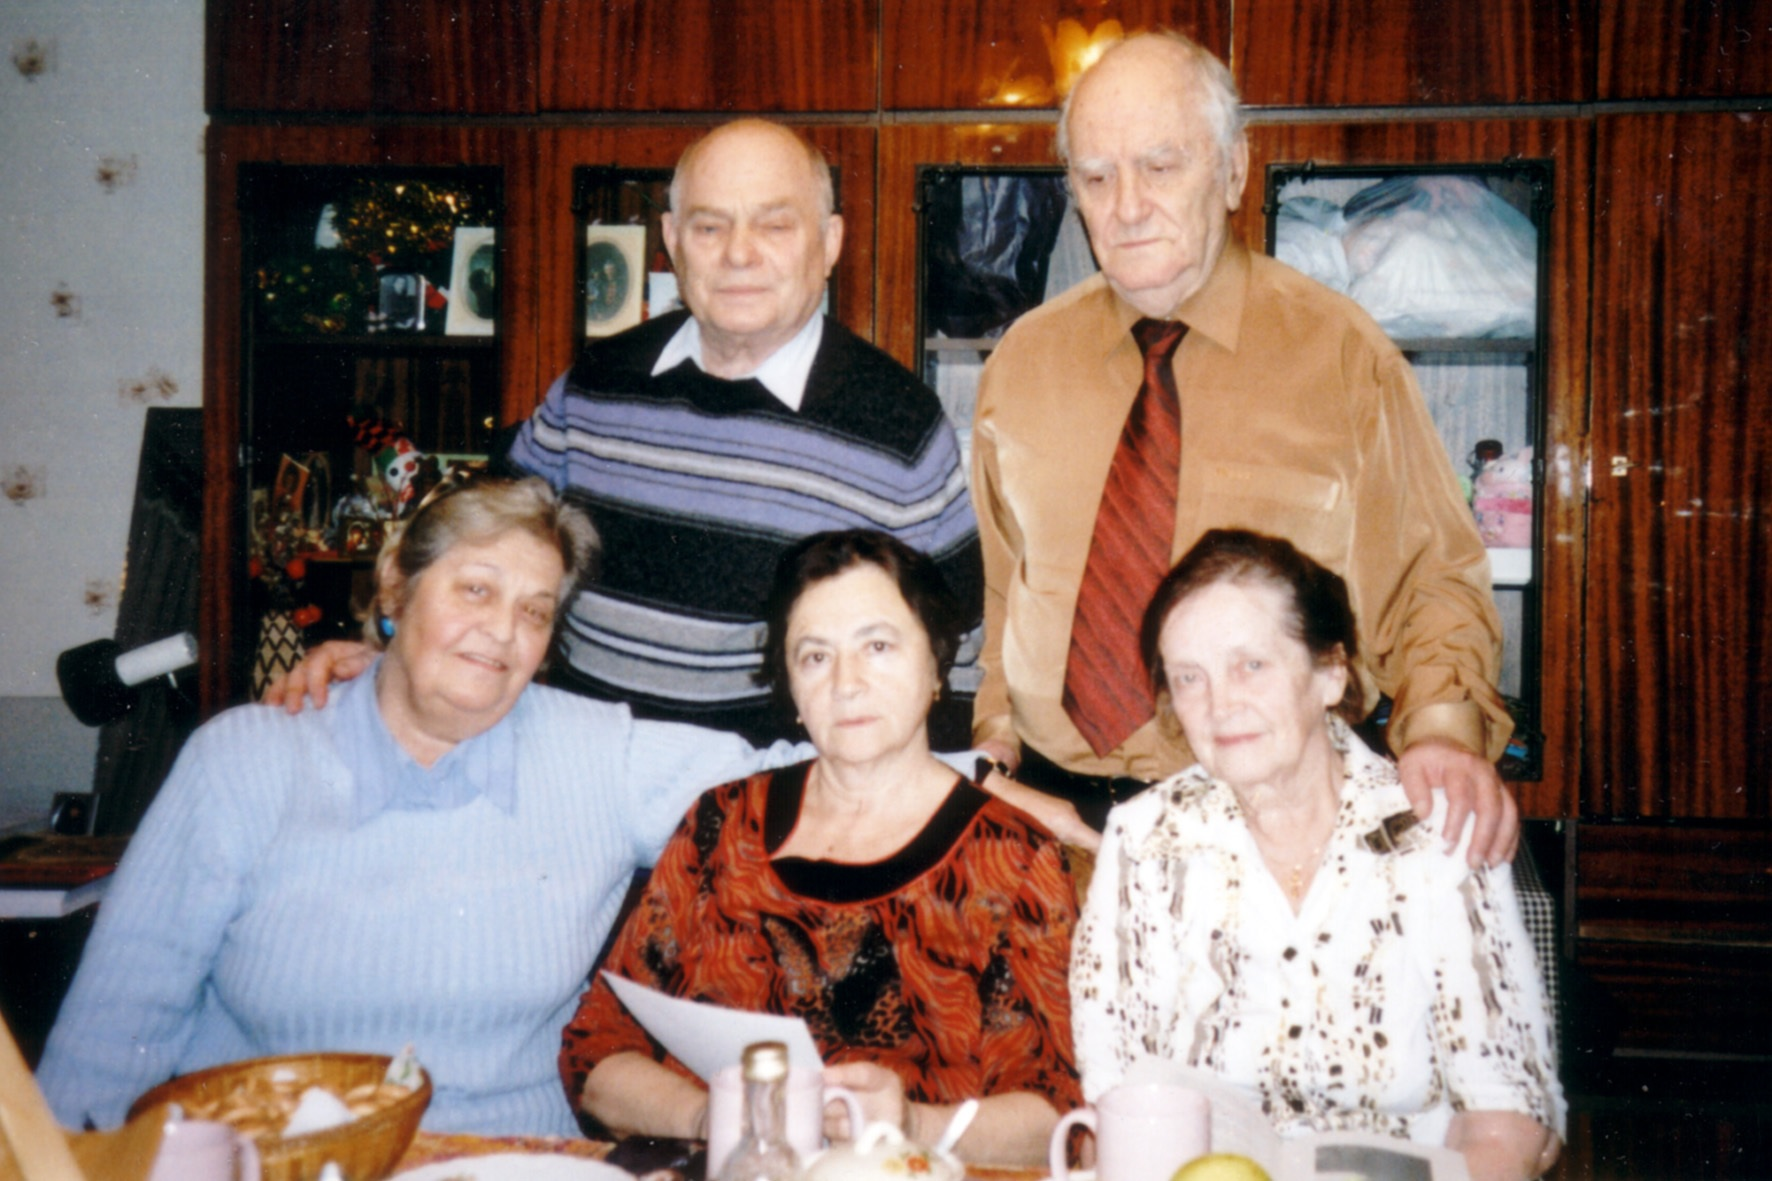
\includegraphics[width=\textwidth]{inc/toAppMinix.jpg}

Только что из книги З. Шейниса узнал о жуткой судьбе отца Миши~-- Марка Абрамовича Плоткина, заместителя заведующего правовым отделом Наркоминдела, члена партии с 1917 г. Один «хороший человек», друг Берии, зам. наркома НКИД Деканозов, пригласил его вечером на беседу, с которой он не вернулся, другой~-- Молотов~-- следующим утром вызывал его из дома для доклада: «Где он?». Вот в такие иезуитские игры играли сатрапы Сталина. М. А. Плоткин в 1939 году был расстрелян как враг народа. В 1956 г. полностью реабилитирован «за отсутствием состава преступления».  

Во втором подъезде жила удивительная женщина и великолепный врач Эсфирь Яковлевна Бару. Она в прямом смысле слова~-- спасла нашего сына. У жены была послеродовая грудница; в роддоме болезнь запустили настолько, что жену с сыном пришлось переводить в другую больницу на операцию. В этой больнице грубо нарушили режим кормления новорожденного ребенка, в результате у него развилась гипотрофия в очень тяжелой форме. Это обнаружила Эсфирь Яковлевна, которая проявила чудеса профессионализма и человеческого участия, чтобы спасти ребенка. Низкий ей поклон.

Марию Михайловну Гюнтер из нашего подъезда я в течение десятилетий периодически встречал на территории Донского крематория, где похоронены ее муж и старший сын, ушедшие из жизни один за другим. Теперь на памятнике и её фотография. Всегда подхожу к ним.

Помню, как Мария Михайловна получала уроки финансового мастерства от моего отца. Даже в очень преклонном возрасте она оставалась красивой женщиной. Я рад, что успел сказать ей об этом.
    
Очень симпатичным мне человеком был Ю. Д. Райский (седьмой, затем четвертый подъезд), но после детства мы встречались, в  основном, случайно. Вот почему. Более поздним моим друзьям\protect\footnote{Б. И. Моргунов, наоборот, относится к ранним друзьям (года с 48-го~-- 49-го), но это совсем другой случай~-- наши семьи, с пафосом говоря, проросли друг в друга, начиная с отцов и кончая детьми. На внуков, правда, это уже не распространяется.}  мне уже было, что предъявить, а в «Юрин период» я еще не созрел, не сформировался, поэтому был ему не интересен… и наши пути разошлись, хотя он был на нашей свадьбе, наши жены вместе гуляли с детьми, он тепло поддержал меня при неприятностях в институте, где он работал. То же относится и к некоторым другим друзьям той поры, вернее~-- приятелям.


Отдельно хочу сказать о человеке, которого мои родители знали с середины 20-х годов по первому дому НКИД\protect\footnote{Она знала многих наркоминдельцев в нашем доме, была частым гостем у нас и у них.}, а я с послевоенного времени – о Марии Михайловне Олькеницкой. Она была красивой, энергичной женщиной, незаурядным, сложным человеком, порой нетерпимым, противоречивым, всегда интересующимся всем, почти без исключения.
 
Выпускник экономического факультета МГУ, она с восхищением слушала лекции Н. И. Бухарина, видела и слышала Маяковского, Есенина, Северянина, Сашу Черного, великих актеров и писателей того и более позднего времени, знала многих художников, даже, кажется, Коровина. Очень интересно рассказывала о событиях и о людях. У меня хранятся подаренные ею альбомы И. Левитана, М. Врубеля, В. Серова  1957- 1959 годов выпуска\protect\footnote{Два последних с хорошими наклейными цветными иллюстрациями (как встарь в «Академии») – не хуже, чем в Белой серии. А Левитану, как и в этой серии, не повезло.}. В одном из этих альбомов я обнаружил ее комментарий к выставке «Сорокалетие Октября».  

Ее первым мужем был талантливый дипломат, расстрелянный в 37-м, вторым – мой двоюродный брат 1900 г. р. Она много знала, многое понимала раньше других, читала и перечитывала любимое до последних дней, по «древней» привычке штудировала газеты, часто присылала мне из Питера или передавала в Москве  вырезки, например,  из «Известий» от 7 февраля 1982 г.  – к 25-летию творчества И. Глазунова.
Относилась она ко мне необычно,  по-своему – очень хорошо. Может быть, это было отражением ее любви к сыну, которого она потеряла еще до войны.

Ходили мы с ней и на выставки, и в Консерваторию. Однажды нам повезло – в Малом зале состоялся вечер Д. Д. Шостаковича и его ученика Г.В. Свиридова. Были авторы. В частности, исполняли удивительные миниатюры «Нарочно не придумаешь» (из «Крокодила»).

Жизненная энергия (скорее, борьба за жизнь) была у нее необычайная. Показательна охота (вынужденная) к перемене мест: окраина Москвы – Центр –  Сокольники – Басманная – Люберцы – Питер (поближе к сестрам) – Лобня. Всё, что накопилось за десятилетия, было растрачено на переезды и на активную жизнь. Больше всего удручали пустые книжные полки. А книги она с мужьями собирала поштучно всю жизн. Gотом стала главным клиентом библиотеки Лобни.

Последнее, что она продолжала стойко хранить, были «каретники» (антикварные часы для путешествия в ночное время: с позолоченными стойками,  хрустальными стеклами, через которые просматривался механизм; с кнопкой для справочного перезвона, а был еще и регулярный перезвон через каждые четверть часа, и ежечасный бой; всё это в солидной кожаной обойме с окошком для красивого циферблата), завещанные мне. Конечно же, они были проданы мною при ее жизни и для нее, а я «выторговал» символическую премию на подарок сыну. Завещание храню.

Заканчивала жизнь она тяжело. Мы с женой старались проявлять сочувствие и солидарность, помогали, как могли.




\chapter{}

\section*{Из воспоминаний C. Л. Корчиковой (Клейн), И. Д. Бабенко, Н. Б. Канторович.}

До войны в 30-е годы в доме № 2/6 по Хоромному тупику существовал Красный уголок для жильцов дома и их детей. Он был организован усилиями энергичного человека~-- управдома Ивана Максимовича Калиша и находился в подвальном помещении подъезда №5. Большую работу по организации кружков вела Евдокия Ивановна Варзар. В Красном уголке постоянно работала библиотека(книги выдавала и беседовала о книгах Елена Николаевна Лоренц), демонстрировались фильмы, тогда черно-белые и немые (регулярно приезжала кинопередвижка), и работали кружки: драмкружок с приглашенным режиссером,   танцевальный   кружок, детский   оркестр; гордостью    Красного уголка стал    кружок автомобилестроения,   в   котором дети под руководством специалиста конструировали     педальные   автомобили   из   фанеры и деталей, которые поставлял ГИРД ( Государственный   институт ракетных двигателей), находившийся в   районе   Красных   ворот;   в этот институт для детей   была проведена  экскурсия,    которая  произвела на  них    большое   впечатление; на этих автомобилях несколько мальчиков и   девочек совершили   въезд  на Красную площадь    в   праздник МЮДа   (Международный   юношеский день 1 сентября).

Красный уголок был местом постоянного общения  детей, где они могли обменяться впечатлениями о прочитанных книгах,    прослушанных   по   радио интересных передачах (телевизоров тогда не было), поиграть на пианино или на бильярде, подготовиться      к очередному концерту: концерты,   на   которые всегда приходили   родители и   другие жильцы дома, готовились    к каждому празднику, ставились спектакли, к которым дети сами шили костюмы и делали декорации,   играл   детский оркестр,   дети     пели, танцевали и читали стихи. К каждому празднику все   дети получали подарки:   небольшой   мешочек   с поздравительной открыткой и -кондитерскими изделиями.

\vfill

Красный уголок стал любимым местом общения детей и их культурного времяпрепровождения и развития.

\vfill

Кроме того, Красный уголок был также местом собраний жильцов дома, общественности, где обсуждались разные насущные проблемы; и просмотр фильмов обычно предназначался совместно для детей и взрослых.

\vfill

В настоящее время, когда дети нередко предоставлены самим себе и не имеют должного общения, представляется очень актуальным возродить заведение типа прежнего Красного уголка и создать условия для его функционирования, предоставив для этого подходящее помещение, а конкретно-свободное подвальное помещение в подъезде № 5 дома № 2/6 по Хоромному тупику.


\begin{figure}[ht!]
    \begin{minipage}{100mm}
        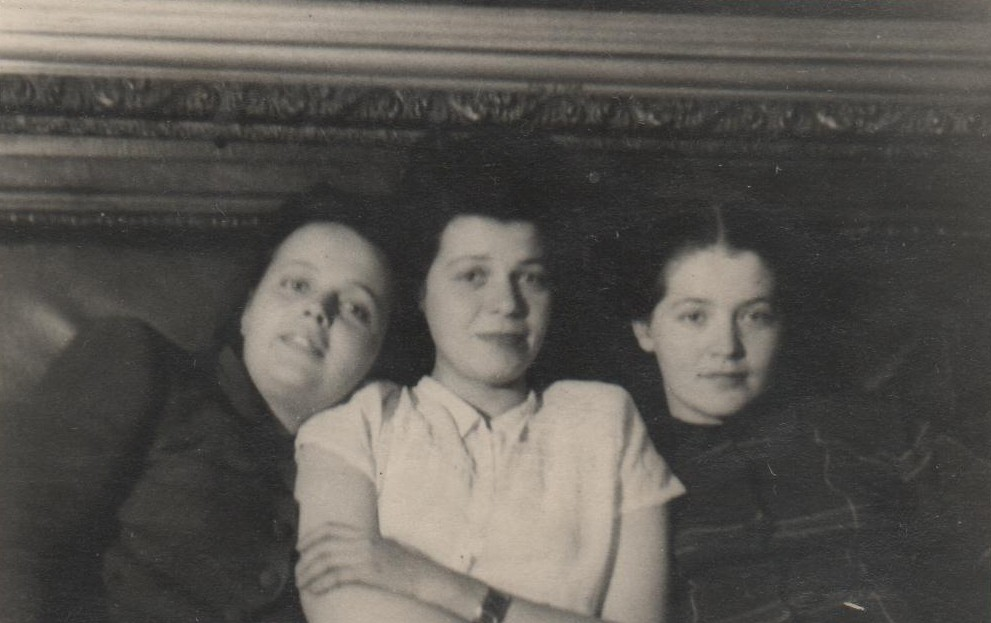
\includegraphics[width=100mm]{inc/p2a}
        \footnotesize{\textit{Соня Клейн, Люба Абрамович, Нина Клейн. Конец 40-х.}}
     \end{minipage}
\end{figure}

\vspace{10pt}

\begin{figure}[h!]
\begin{minipage}{100mm}
    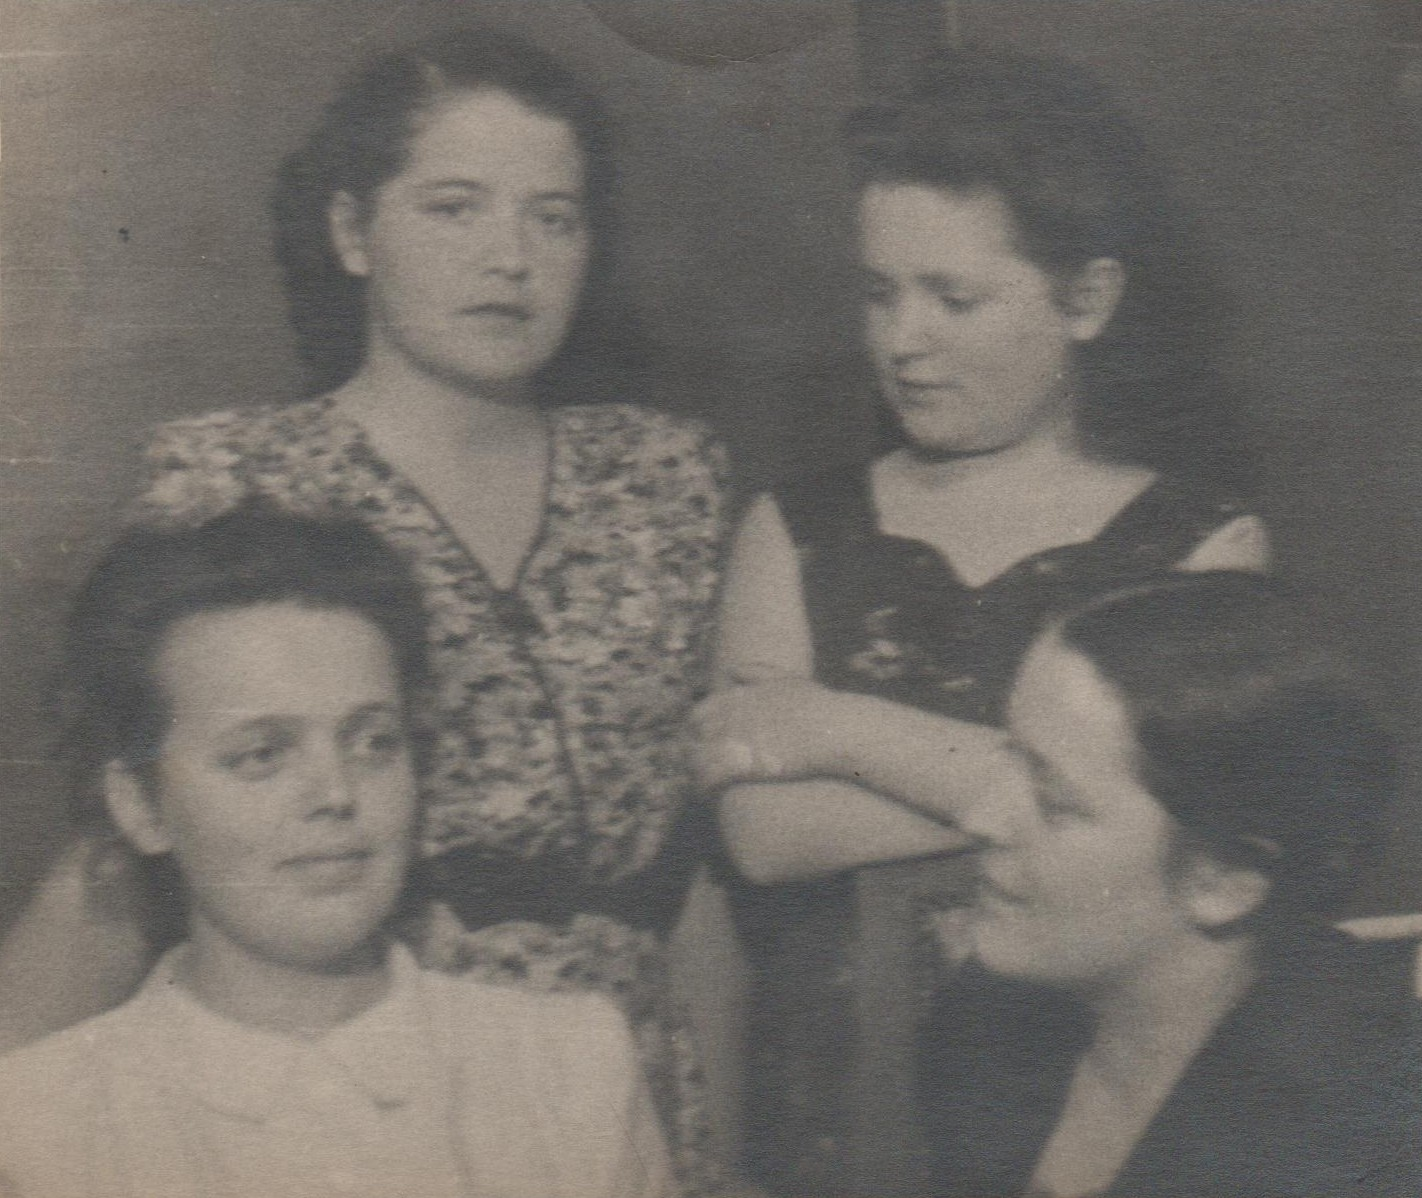
\includegraphics[width=100mm]{inc/p1a}
    \footnotesize{\textit{Сестры Клейн. Соня, Нина, Анжелика (Лика), Наташа (Туся). Конец 40-х.}}
\end{minipage}
\end{figure}


\chapter{}
\section*{Из воспоминаний Н.Б. Левданской (Канатрович)}

Я родилась  в  1923 году  в  Москве. Наша  семья  занимала  две  комнаты 
коммунальной  квартиры  в  доме  №21  на Кузнецком мосту,  там,  где  памятник 
Воровскому.  Два  подъезда  этого жилого  дома~-- №№  6 и 7~-- занимал Наркомат 
иностранных дел, где служили мои родители.

Мама~-- Бетти  Моисеевна  Канторович  (Маркус)  была  машинисткой, а отца~-- 
Бориса  Ильича  Канторовича~-- приняли  на работу по рекомендательному  письму 
Ленина Чичерину. Дело в том, что папа после того, как окончил гимназию с  золотой 
медалью  в Гомеле,  где жила  его  большая семья (у бабушки Розы было 4 сына и 3 
дочери), поступил в университет  г. Льежа (Бельгия),  кстати, самый  дешевый  в  то 
время  в  Европе.  Туда  приезжал  из  Швейцарии  Ленин,  который  вел  беседы  со 
студентами  Русского  землячества.  Вернулся  в  Москву  папа  в  том  же 
запломбированном ленинском вагоне. Попал  он туда благодаря своему  маленькому 
росту, как подросток~-- сын одной из уезжавших семей.

Отец  был одним  из организаторов структуры Наркоминдела,  наших  посольств 
в других  странах.  По работе он занимал разные должности,  был  членом  коллегии 
Наркомата.

В конце  20-ых годов, когда  Наркоминдел  стал  расширяться  и  должен  был 
занять весь дом,  а жильцы расселены, встал вопрос о строительстве кооперативного 
дома, что и было сделано  совместно с другими организациями.  В апреле  1929  года 
мы переехали в дом № 2/6  по Хоромному тупику  в пятикомнатную квартиру № 64. 
К нам с Арбата переселилась бабушка Таня, мать мамы.  В этот же дом переселилась 
сестра мамы Елена Моисеевна Маркус  с  мужем  Леоном  Яковлевичем Гайкисом, 
тоже наркоминдельцы.

После коммуналки дом был  воплощением мечты: отдельная квартира,  ванная, 
газовая  плита. Для  детей  были открыты детский сад  в  квартире  первого  этажа 
в подъезде № 2, замечательный Красный уголок в подвале  5-го подъезда,  где  были 
библиотека, кинопередвижка,  разные  кружки. Для  хозяек к дому был  прикреплен 
гастроном  № 3: по телефону можно было заказать продукты, а  после работы  взять 
их в специальных ячейках, сделанных в стене входной арки.

В  1930 г.,  в связи с  индустриализацией страны, было указание  о переводе  в 
промышленность  работников  с  техническим  образованием.  А так  как  папа был 
инженером по строительству дорог и мостов, он был  направлен в ЦУДортранс и два 
года работал  по  реконструкции  Военно-Грузинской дороги. Мама же  после НКИД 
поступила во Внешторгбанк на должность иностранного корреспондента, т.к.  знала 
несколько языков.

В эти же годы родители вступили в дачный кооператив  и  получили  маленькую 
фанерную дачку близ платформы Валентиновка Северной ж.д.

Период  1935-36 гг  был  тяжелым.  ЦУДортранс  ликвидировали,  т.к.  его 
руководство проходило по процессам,  работы  не было, материально было трудно. 
Немного  помогал Торгсин,  куда  отнесли золотые  медали  родителей,  кое-какие 
бабушкины вещи.  В конце концов  папе  удалось  устроиться  в  плановый отдел 
Мострамвайтреста.

Л.Я. Гайкис  продолжал работать в Наркоминделе  и  в 1935 г. был  направлен 
генконсулом посольства в Турции, куда отправились  всей семьей: тетя Лена  и  две 
их дочки:  Наташа, родившаяся в  1930 г., и Оля  1934 года рождения.  Свою квартиру 
они  передали Е.В. Голубевой, вдове  И.А. Дивильковского, которого знали по НКИД. 
Гайкису  в дальнейшем  была обещана  квартира  в новом кооперативном доме  на 
Каляевской.  В начале  1937 г. Леон Яковлевич  получил  назначение  на  должность 
посла  в Испании  и отправился  в Мадрид,  а семья  из-за  войны  поселилась  во 
Франции, где тетя Лена стала работать в нашем посольстве.

Наступил страшный  1937 год. Каждую  ночь  люди  НКВД  на черных  <<эмках>>
увозили арестованных.  23 мая  эти  люди  пришли к нам. Был  обыск, и на рассвете 
папу увели, оставив  нам номер  ордера  и опечатав  все  пять комнат. Маму после 
этого  парализовало,  мы  с  домработницей  Маней  вывезли  ее  кровать в  коридор. 
Мама лежала без медицинской помощи.

Мы  остались  без  самых необходимых  вещей. Предстояла зима,  а  у  нас  вся 
теплая одежда оставалась в запертых комнатах. Я пошла к  прокурору.  Он сказал: 
<<Если хотите остаться живыми, уезжайте из Москв>>.  И  дал  указание  открыть 
на время  одну-две  комнаты, чтобы  мы  могли  взять  необходимые  вещи.  К  нам 
пришел человек, и под его надзором  мы с  Маней  взяли  самое необходимое. Один 
раз мне удалось проникнуть в  опечатанную  комнату без  надзора. У нас с соседями 
был общий балкон, перегороженный сеткой, я  с их разрешения через нее перелезла, 
с помощью  форточки  открыла  окно,  влезла  в  бабушкину  комнату  и  взяла  из 
буфета серебряные  ложки и подстаканники.  Слава  Богу, что  бабушка  не  видела 
всего этого: ее не стало в феврале  1936 года.

В школе я сдала экзамены за шестой класс, и  мне помогли  перевезти  маму  на 
нашу  дачу в Валентиновке.  Отношение  людей  к нам  было  разное:  кто  помогал, 
кто сочувствовал, а кто при виде меня переходил на другую сторону улицы.

В этом  1937 году в Харькове и  Киеве  арестовали  трех  братьев  отца  вместе  с 
женами.  Мужчин  расстреляли,  женщины,  кроме  моей  мамы,  вернулись,  но 
инвалидами.

Л.Я. Гайкиса  тоже  не  миновала  эта  участь:  в  июле 1937 г.  его  отозвали  в 
Москву  и арестовали в гостинице «Москва», где он остановился. Тетю Лену  тут же 
уволили с работы и отправили в Москву, куда она с девочками  и  прибыла. Но  жить 
было негде; тогда  Лена вместе  с Ниной  Исидоровной  Мельниковой (с той же судьбой)
сняли комнату в  деревне на станции Калистово в Подмосковье.

В домоуправлении мне выдали справку, с этим документом  я ходила  по  разным 
инстанциям. О папе можно  было  узнать в справочной  НКВД  на  Малой Лубянке. 
Очереди были огромные. Не  всегда подойти  к окну удавалось  за  весь день,  тогда 
мы оставались  на следующий.  На  этой улице  тогда  был  небольшой  костел,  туда 
пускали на ночь.  Каких  трагедий  я  навидалась  в  этих  очередях~--- не передать... 
Подойдя к окну,  надо  было  назвать  номер  ордера, фамилию  и дать  3 рубля  ( на 
курево заключенному); если деньги брали,  это  значило, что  человек жив.  У меня 
там взяли  в июне  и в июле, а  в августе  мне это удалось  в Бутырках,  т. к.  Малую 
Лубянку закрыли.

Когда  в сентябре  отняли  и  нашу  маленькую  дачку,  наша  домработница 
Маня  предложила нам поехать  на ее родину  в  город Углич.  Маня  съездила туда, 
нашла нам комнату  и  потом  приехала  за  нами.  В  30-е  годы  в Угличе строили 
гидроузел, и  там  провели  железную  дорогу  от  Калязина  до  Углича (40 км). 
Доехав из Москвы  до Калязина, мы перебрались в вагон-теплушку,  поставили там
мамину  кровать, так  добрались  до Углича и  сняли  комнату,  которую  Маня нам 
заранее подготовила. В Угличе я  начала  учиться  в седьмом  классе  и работать  в 
школе, а  мама, когда  поправилась,  поступила  на  работу  счетоводом  в  артель 
инвалидов.

Каждые каникулы я ездила в Москву, ходила  в справочное  НКВД  на Кузнецком 
мосту,  в  прокуратуру  на  Пушкинской  улице,  и  везде  получала  ответ:  «10 лет 
строгого режима без права переписки».  Тогда мы  еще  не  знали, что это означает~-- 
расстрел.  Когда  через  много лет, в 1992 году, я  прочла  дело отца, я узнала, что 31 
октября 1937 г. был суд, продолжавшийся  18 минут, а 1  ноября отец был  расстрелян.

В  1939 г. в деревне  Калистово  была  арестована  Н.И. Мельникова,  тогда  мы 
решили  поскорее забрать тетю Лену с девочками  в Углич.

В  1939 -- 40-м годах  я  ездила на летние каникулы  в  Харьков, где папина сестра 
собирала  на  отдых  нас, племянников-сирот.  Там  я  познакомилась  с  прекрасным 
парнем Наумом Соколовским, семья  которого сыграла большую роль  в моей  жизни. 
Мы  долго переписывались, а 21  июня 1941  года, когда я окончила школу, он приехал 
в Углич, чтобы забрать меня в Харьков, где я могла бы продолжить свое образование. 
Но на другой день началась война, и он сразу уехал, т.к. дома у него  была повестка в 
военкомат. Забегая вперед, скажу, что  он достойно воевал  и погиб  в  1943 году  под 
Гомелем. В  1967 г., получив  известие от  его матери, которая  после долгих поисков 
узнала место захоронения сына, я приехала в деревню  Барсуки, где  встретили меня <<красные следопыт>>~-- школьники 5~-- 6 классов, которые занимались поисками мест 
захоронения. Меня проводили в лучший по тем временам дом,  где  меня  с  большой 
теплотой приняла хозяйка  и подарила  мне кусочек драгоценного  для того  времени 
мыла. Но как велико было мое изумление  и моя радость, когда она  разыскала  среди 
многих  полуистлевших бумажек мое письмо, написанное  моему  жениху!  Красные 
следопыты  вместе с односельчанами  привели меня к братской  могиле, на  которую 
я  положила цветы.

В Угличе на второй  день войны, 23 июня, меня послали  от  горкома комсомола 
проводить собрания в колхозах. Когда я возвращалась домой, меня встретили друзья- одноклассники  и  сообщили, что  маму  увезли  в  больницу.  Но, когда  я  увидела 
опечатанную дверь комнаты, я поняла, что случилось, и бросилась  к дому, где  жила 
тетя  Лена  с  детьми. Там  в это  время  шел  обыск,  меня  не  пустили,  попросту 
выкинули в коридор. Детей на это время  приютили  соседи. Я пошла в отдел НКВД, 
комнату мне вернули и разрешили девочек  взять к себе, т.к. мне уже исполнилось 18 
лет.

Потянулись  страшные  военные  дни. Осенью Наташа пошла  в школу, а Оля~-- в 
детский  сад. Было холодно (дрова на рынке  стоили дорого) и голодно,  ведь нам  не 
давали хлебных карточек, как детям «врагов народа». Правда, в  горкоме  комсомола 
в буфете раз  в неделю мне давали буханку хлеба. Ходила по деревням, меняла вещи 
Лены (своих не было) на муку,  на картошку. Работала я в школе,  летом  с  ребятами 
в  поле помогали колхозу, а осенью нас, взрослых,  возили  на  рытье  окопов,  ведь 
немцы  были близко.

Пыталась найти  маму и Лену. Посоветовали писать в отделы НКВД ближайших 
областей. Осенью ответили из Ярославля. Добралась я туда  с трудом, т. к.  никакого 
регулярного  сообщения  не было,  а попутные грузовики  брали  только  за  махорку 
или водку. Там  я узнала,  что  мама  и  Лена  вместе, следователь  уговаривал  меня 
сдать девочек в детдом, но об этом я даже думать не могла.

Так прошел первый тяжелый военный год.  Наум Соколовский  регулярно  писал 
с фронта,  и  с его родителями я тоже переписывалась.  Они были  в  армии, но  не  в 
строевых частях. К маме и Лене ездила несколько раз, отвезла им теплые вещи.

Летом  1942 года за нами приехал отец Наума Иосиф Яковлевич и отвез меня  с 
девочками в город  Рыбинск, где  расположилась  военная база, и мы стали  жить в 
этой  гостеприимной  семье.  Иосиф  Яковлевич имел звание капитана, а  жена его~-- 
Евгения Наумовна~-- была  вольнонаемной.  Я  опять  работала  в  школе, девочки 
учились.  Так  получилось,  что  лагерь, где  были  мама и Лена,  тоже оказался  в 
Рыбинске.  Я  могла  иногда издали  наблюдать, как  их этапом  ведут  по городу от 
зоны  к  Волге,  и  с  ужасом  видеть, что  моя  мама, инвалид,  по  колено  в  воде 
вылавливает  плывущие доски. Единственное, что  мне  удавалось,~-- это  передавать 
им через проходную  кое-какую еду.

Встал  вопрос  о моей  дальнейшей  учебе.  Дважды  я  посылала  в  разные 
московские вузы свои документы, и  все они, несмотря  на <<золотой>>  школьный 
аттестат,  возвращались  обратно.  Тогда  моя  двоюродная  сестра,  студентка 
строительного  института,  придумала  мне  подходящую  биографию  и  вместе с 
аттестатом  отнесла  в  МИСИ.  И  ведь  приняли!  Соколовские  отпустили  меня, 
оставив  девочек  у себя,  и осенью  1943 года я оказалась в Москве.

Прописали меня в общежитии на Извозной улице, но там  было  трудно жить  и 
заниматься. В здание попала во время налетов бомба, его еще  не отремонтировали, 
окна были забиты  фанерой, вместо лестничных маршей лежали доски, поэтому там 
я  жила не постоянно, а <<скиталась>>  по городу, пользуясь гостеприимством  друзей 
и  знакомых.

В  1944 году  нам  с  двоюродной  сестрой,  студенткой-медичкой,  дальние 
родственники дали  возможность временно  пожить  в пустующей  комнате (хозяин 
был на фронте) коммунальной  квартиры  на  Домниковке.  Хотя  было холодно  и 
голодно, мы были  рады. Подружились  с  соседями.  Там же  я  познакомилась  с 
моим  будущим мужем  Максимом  Ильичом  Левданским.  Он  воевал,  был  ранен 
и  контужен  под Сталинградом,  прошел  несколько госпиталей,  последний  был 
в  Москве.  Нашему  соседу он был другом детства.

Девочки  оставались  у  Соколовских.  Из  Рыбинска  военную  базу перевели  в 
Можайск, куда я ездила по выходным, а потом в город Ржев. Лагерь, где были мама 
и Лена, тоже  <<переезжал>>: война  отходила  на запад, нужна была рабочая сила для 
восстановления  разрушенных дорог,  домов  и  прочего  хозяйства.

В январе  1945 г.  неожиданно  тетю  Лену  из  лагеря,  который  в это  время был 
в Уваровке (недалеко от Бородино) привезли  в Москву.  Освободила её организация 
<<Польские патриоты>>, которая искала людей для освобожденной от немцев родины, 
а фамилия  Гайкис  была известна  в  Польше. Жить  было негде, но есть  хорошие 
люди: Лену и девочек, которых  Соколовские привезли  из Ржева, взяли  к  себе  в 
одну комнату коммуналки  старые друзья.  В июне  1945 г. был сформирован  целый 
эшелон  из  людей, в основном, найденных в Гулаге, и отправлен в Варшаву.

А  я в сентябре  1945 года  вышла  замуж  за  М.И. Левданского  и  поселилась  в 
Томилино, где он жил с мамой. Наконец я обрела крышу над головой и нормальную 
жизнь. У нас  была половина дома (две комнаты и терраса  с  удобствами на улице), 
но все равно  это счастье.

В  1946 г. у меня родилась дочь Таня,  в  1949 г.~-- сын Илюша.

Доучиться  в  МИСИ  не  получилось,  свое  образование  я  заканчивала  через 
несколько  лет  заочно.  Надо  было  растить  детей,  к тому  же  свекровь  серьезно 
заболела и в августе  1948 г. скончалась. По страшному совпадению  в этот  же  день 
не  стало  моей  мамы.  Из  лагеря пришла  обратно посылка с наклеенной бумажкой. 
Случилось  это в Горьковской области. Маме было 53 года.

В  1951  г. с помощью моих сокурсников, ставших уже инженерами, я  поступила 
в  проектный институт, в котором проработала до пенсии, постепенно  <<поднимаясьпо  служебной  лестнице>>,  дойдя  до  должности  главного  инженере  проекта.
Обстановка  была рабочая, коллектив прекрасный (общаемся до сих пор).  Я  много 
ездила в командировки~--- и  на выбор площадок под строительство, и  на  авторский 
надзор.

Соколовские  после  войны  вернулись  в Харьков. Мы все~-- и я, и муж, и  дети~--
ездили к ним, один раз вместе с Олей,  которая приехала из Варшавы, помогали  bм 
продуктами, лекарствами, деньгами вплоть до их кончины.

Жизнь в Томилино шла своим чередом. Дом постепенно улучшался:  пристроили 
кухню,  утеплили  террасу. На  участке  росkb  вишни,  малина, смородина; был 
небольшой  огород,  цветы.  Но все  это  рухнуло,  когда  а  октябре  1963 года  от 
обширного  инфаркта  скоропостижно,  во сне. скончался  муж.  Случилось  это  в 
Крыму, в доме отдыха. Максиму Ильичу было 5O лет.

Осиротели  мы  с ребятами. Жить  стало трудно, пенсию  на  детей  по  утрате 
кормильца назначили~-- 38 руб.43 коп.  Хваталась  за  любые  подработки,  дети 
помогали. Они у меня замечательные,  школу окончили  оба  с  золотой  медалью  и 
поступили в институты.

После  смерти  мужа  тяжело  было  содержать  наш  дом. и потребовался год 
неимоверных усилий, чтобы обменять его на небольшую  двухкомнатную квартиру 
с удобствами. Активно помогали нам с хлопотами сослуживцы мужа и  сотрудиики 
моего  института.  Так  мы  стали  жить  в  пселке  Института  горного дела  им. 
Скочинского, это рядом с Томилино.

Шли годы, дети повзрослели, создали свои семьи:  в 1968 г. Тамя  вышла замуж 
за  своего  одноклассника  Костю,  а  в  1970 г.  Илья  женился  тоже  на  своей 
однокласснице Миле. Все  четверо окончили  вузы, стали  работать. И зять и  сын 
отслужили  в  армии. Родились внуки.  И  а решилась  а 1975 г.  вторично  выйти 
замуж.  С  Михаилом  Ивановичем  Касьяновым  я  проработала  вместе  более  20 
лет. Он в свое время прошел ГУЛАГ, овдовел,  был  на  пенсии.  В его семье  тоже 
были дети, внуки, причем дочь замужем за М. М. Плоткиным  (он из нашего  дома  в 
Хоромном), тоже сыном <<врага народа>>.

В 1978 г. я вышла на пенсию,  пришло время  помочь  детям.  Четверо  внуков 
пошли в детский сад, нужно было их приодеть. Купить в те годы было нечего,  и  я 
стала  портнихой.  Из  взрослых  ношеных  вешей  перешивала  внукам  платьица, 
юбочки, брючки и проч.

С опытом  дело  пошло  лучше,  и  вскоре  я  стала  <<обслуживать>>  и  своих 
взрослых детей. Мне всегда хотелось научиться шить, но не было времени,  к тому 
же  с  уходом  на  пенсию я получила от сослуживцев в подарок швейную  машинку 
с  электроприводом.  Она  и  сейчас  выручает, правда,  нового  почти  не  шью, в 
основном, заплаты и переделки.

С  Михаилом Ивановичем мы прожили  почти  13 лет. За  эти  годы побывали с 
ним, кроме  Подмосковья,  в разных местах: в Карпатах, в Одессе и Черновцах,  на 
Валааме. Первое  время  мы  жили  с семьей  его сына  в доме  у Чистых  прудов, а 
затем  нам  дали  однокомнатную квартиру в доме на ул. Новая дорога, где  я живу 
до сих пор. Так снова я стала  москвичкой,  да еше  и  в родном  Бауманском (ныне 
Басманном) районе.

Уже 2S лет, как  нет  Михаила  Ивановича;  с  его  семьей  у  меня  прекрасные 
отношения,  мы  перезваниваемся,  встречаемся,  вместе отмечаем разные  события.

Жизнь  так повернулась,  что  я  получила многое,  что было отнято.  У  моих 
детей  большие  семьи.  У дочки  Татьяны  Максимовны  с мужем  Константином 
Анатольевичем  сын Сергей,  у которого с женой Катей  двое детей, и  дочь Ольга  с мужем  и  сынишкой. У сына  Ильи Максимовича с женой  Людмилой  Евгеньевной 
две дочки~--  Маша и Наташа,  два  зятя~--  Антонио  и  Александр  и четверо внуков.

Все  мои  дети  и  внуки получили  высшее образование,  все  работают  (кроме 
дочки и невестки, которые вышли на пенсию и воспитывают своих  внуков).

Мое  продолжение~-- правнуки.  Старший~-- Саша~--  пойдет  в  восьмой  класс, 
две девочки~-- Вероника и Соня~-- в четвертый,  два  мальчика~-- Максим  и  Миша~-- 
первоклашки, и двое маленьких, ясельных,~--  Петя и Бейка (Беатриче).

Вот  такая  гвардия!  Если же  прибавить внуков и правнуков  Касьяновых,  то 
получается огромное число.

Я живу  одна,  но  одинокой  себя  не считаю. Мои  частенько  навещают, и  я 
езжу  к  ним,  стараюсь  хоть  чем-то помочь,  делаю  все  дела по  дому,  читаю, 
смотрю  телевизор  (в основном, «Культуру»),  стараюсь  не  отстать  от  жизни. 
Конечно, бывают  и  грустные  мысли:  самая  большая  боль  I  что  нет  могил 
родителей,~-- и нездоровье, но я не сдаюсь.

Оглядываясь  назад, вижу, что в  моей  долгой, почти  девяностолетней  жизни 
было  много  страшного,  трагического,  но,  к  счастью,  и  немало  хорошего. 
Встречались прекрасные люди, понимающие, помогающие. Вот так и выстояла.

В  1957 г.  после  XX  Съезда  все  семьи  Канторович  и  Гайкис  были 
реабилитированы.

Хочу  немного  добавить  о семье  Гайкис.  В Варшаве Лена пошла работать, а 
девочки учились. Все  они приезжали в Москву и хотели,  чтобы  и  я навестила их, 
прислали  приглашение, но  ОВИР отказал  с  формулировкой:  <<Не прямая родня>>. 
Было очень обидно.

После школы девочки окончили университет, создали  семьи,  родились  дети~-- 
и все  кончилось, когда  Гомулка выслал  из  Польши  всех евреев, буквально в 24 
часа.

Лена и  семья  Наташи  перебрались  в Израиль. Там вскоре ушли из жизни~--  и 
Наташа (ей было 43 года), и тетя Лена.

Оля с мужем и дочкой уехали в  Америку,  где  получили  работу в Йельском 
университете  на кафедре  русского языка  и литературы.  Оля проработала там 30 
лет, сейчас на пенсии. После смерти мужа перебралась  в Нью-Йорк, а дочка ее~--  в 
Вашингтоне с мужем и двумя девочками-студентками,  хорошими спортсменками. 
Оля с мужем много раз приезжали ко мне, сейчас регулярно перезваниваемся.

\chapter{}

\section*{Из воспоминаний Э. И. Певзнер.}

Почти 30 лет, со дня моего рождения~-- в 1935г. и до почти 1965г., когда моей доченьке Юле исполнилось 4 года, я прожила в моем любимом, обожаемом дома на Хоромном, у Красных ворот. Этот дом был совершенно особым, со своим миром, со своими законами.

Моя мама, Тейтельбаум Мария Исааковна, вернувшись в 33 году из Бермена, где она работала в Советском Торгпредстве у наркома Литвинова, заплатила (по ее словам) <<золотой валютой>> за трехкомнатную квартиру. Впоследствии, уже перед войной, квартиры перестали считаться кооперативными, и к нам в большую комнату подселили семью~-- из двух человек~-- оба партийцы. Андрей Владимирович Мякишев и его жена~-- Макагон Александра Васильевна. С ними я прожила 25 лет, очень дружно.

Дом наш был построен в виде печатной буквы П, где перекладина была обращена во вне, а все остальное~-- семь подъездов~-- помещались внутри. В дом можно было попасть только через огромные чугунные решетчатые ворота, которые в то время не запирались, и мы, дети, любили на них кататься. После ворот шла довольно длинная арка. До войны на правой стене (от ворот) помещались большие и глубокие ящики с деревянными дверками~-- туда <<особо ответственным товарищам>> доставляли продовольственные заказы. А таких жильцов, особенно до войны, было большинство. По другую сторону арки была каморка с окном~-- сторожка, где всегда сидел дежурный лифтер.

Внутри дома был маленький, уютный дворик, в середине круглый фонтан, потом пристроили песочницу для малышей, а для больших~-- был сколочен простой деревянный стол и две скамейки-лавки по бокам.

И вот настали страшные 37--38 годы. Из 95 квартир нашего дома 60 были опустошены. Людей очень уважаемых в стране, ответственных работников забирали, как правило, по ночам. Объявляли приговор: <<10 лет без права переписки>> (что на деле означало расстрел). Состав дома переменился.

Многие, когда началась война, уехали в эвакуацию. Но в 43 году почти все, оставшиеся в живых, вернулись. В том числе и наша семья. В этом же году я пошла в школу (613-ю женскую~-- первый опыт).

Но вся моя жизнь, как и жизнь всех, проходила в доме, во дворе. Мы дружили~-- целыми поколениями, по возрасту. <<Нашего брата>> было тогда довольно много: Миша Плоткин, Лева Месежников, Боба Моргунов, Галя Столяровская (на год моложе), Рита Гиргидова и Инна Платонова (обе на год старше), сюда же примыкали Женька Займовский, Марик Миникс, а вот Юрка Верещагин, Юрка Райский и Левка Меньшиков считались как бы уже в другой компании [Немного не так. М.М.].  Мы самозабвенно играли в Молодогвардейцев.

Были еще и <<большие ребята>> (так мы их называли). К ним я~-- бойкая девчонка~-- пристраивалась каждый вечер когда они~-- Альчон Горностаев, Шурик Штейнберг и др. тайком поднимались через чердак 5-го подъезда и выходили на крышу~-- смотреть салюты. И как только я, малявка, не сверзилась тогда и не разбилась вдребезги!

Вся жизнь наша шла во дворе, у всех на виду. <<Большие ребята>>, сидя за столом во дворе, в 1947 году читали вслух только что вышедшие в издательстве <<Советсткий писатель>> <<12 стульев>> и <<Золотой теленок>>. Мы, младшие, умирали со смеху и знали их наизусть. (Кстати, потом книгу сразу же запретили~-- и до смерти Сталина она больше не издавалась.)

Главным <<книгочеем>> нашего дома считалась Леля Александровская из 3-го подъезда. Она постоянно просиживала во дворе с книгой в руках, не вынимая изо рта большой палец, который сосала. А на столе часто ставили патефон, и <<большие ребята>> кружились со своими сверстницами. Точно, как по песне Окуджавы о Леньке Королеве, но нам завидовать им было некогда.

Из досок мы устроили качели и, стоя, подлетали прямо под кроны деревьев. Почти каждый день играли в лапту, в штандер, а особенно любимой была игра в казаки-разбойники. Прятаться бегали аж на <<задний двор>>, где была помойка (никаких мусоропроводов в помине не было, все выходили с ведрами и выносили их на задний двор). Дом наш был удивителен еще и тем, что все были свои, т.е. не было никаких пришлых, никаких хулиганов.

<<Чужими>> были только два друга~-- Юлька Зайчик, двоюродный брат Женьки Займовского, да Юрка Епишин из соседнего, бандитского дома,~-- оба безнадежно влюбленные в мою подругу Инну Платонову. Инка была тихой, скромной, неразговорчиво девочкой. Отца ее посадили, мать тоже, в комнату после войны приехала какая-то Зоя, обещавшая матери воспитывать Инку. Жили они в квартире 55, прямо напротив нашей 54-й на 6-ом этаже в 4-ом подъезде. Вообще, если рассказывать только о жильцах нашего подъезда, так это~-- целый том.

Сколько себя помню, мы целые дни носились друг к другу~-- я на третий, к Бобке Моргунову, он~-- ко мне. У нас с ним была страсть к книгам, особенно в то время к научной фантастике. Ежедневно мы виделись с Галкой Столяровской и Левкой Месежниковым из 52-й квартиры, как раз под нами. С мамой Левки~-- Ией Михаиловной и Галкиной мамой~-- Бэбой Матвеевной я могла говорить обо всем, почти как с родителями. На четвертом этаже жили Рабиновичи~-- чудесная, добрейшая Елизавета Ефимовна с двумя сыновьями~-- Эмиком и Натиком. Потом, подрастая, я очень дружила с их женами~-- Таней и Валей. А Валину дочку~-- очаровательную белокурую Инночку с личиком ангелочка~-- учила игре на фортепиано моя любимая подруга Маша, когда  мы с ней были студентками иняза. Она~-- Инночка~-- почти <<последняя из Могикан>>~-- до сих пор живет в старой квартире. Чудо! Напротив них, в квартире №50 жил знаменитый Штейн~-- зам. Молотова, в ранге посла.

Помню время перед смертью Сталина~-- самый разгул антисемитизма. Я ничего не понимала, верила, дура, газетам. Встречала его, без погон, в подъезде, страшно подавленного, но, слава Богу, не посаженного. А его жена преподавала на дому вокал. И когда бы ты ни шел по подъезду, всегда раздавалось это а-а-а-а-а-а-а! Это никого не раздражало.

На 3 этаже жили Кунины~-- очень славные. А на 2 этаже~-- уникальная личность, как говорили у нас тогда, друг Ворошилова~-- Иона Каменский. Рассказывали шепотом, что на голове у него какая-то огромная штука. Была у него взрослая дочка~-- Ирка Каменская. Все называли ее Камека. Считалось, что она сверхэкзальтированная девица. Рассказывали, что папаша бьет ее смертным боем, а она выскакивала во двор, ложилась на пол, орала и считалась истеричкой, а вообще она, наверное, была несчастное создание, рано лишившееся матери.

Еще я очень хорошо помню трех молодых людей, просто трех мушкетеров, из хороших, благовоспитанных семей~-- Алика Гриневского из 1-го подъезда, Вовочку Андреева из 2-го и Сергея Дивильковского из 3-го. Мы необидно называли их (по порядку)~-- Спичка, Супчик и Кашка. Все трое потом стали знамениты: Алик~-- посол (после МГИМО), Вовочка~-- народный артист, художественный руководитель театра Ермоловой, а Сергей, закончивший МГИМО,~-- крупный дипломат.

Вообще, люди в нашем доме были замечательные. У нас жил в 6-ом подъезде ставший знаменитым детский писатель Юра Коваль. В 5-ом подъезде жили сестры Клейн~-- все с медицинским образованием. В 1-ом подъезде до сравнительно недавнего времени жила знаменитая переводчица со скандинавских языков и писательница~-- Юлиана Яхнина.

И красавицы у нас были такие~-- просто глаз не оторвать. Например, в 5-ом подъезде, сразу же после войны, проживала расфранченная дама Элеонора Борисовна Крейндлина с дочкой Лорочкой~-- принцессой с голубыми глазами и золотыми кудрями. В 7-ом подъезде жила девочка уникальной внешности: с ресницами на полметра и прекрасными карими глазами~-- Туся Еременко. К ней тяготела ставшая красоткой Анечка Вайнштейн.

Для меня, девчонки войны, вобравшей в себя всю любовь к Родине и товарищу Сталину, самое интересное время после войны было в Красном Уголке. Находился он в 5-ом подъезде, где для него отвели подвал. Там была хорошая сцена и зрительный зал. Почти ежедневно там крутили все любимые наши фильмы тех лет~-- и все их мы смотрели десятки раз, и все бесплатно.

Работали там и кружки: хоровой, драматический, танцевальный. Я, конечно, была их активным членом. Возглавляла всю самодеятельность некая Ангелина Сергеевна Спартак~-- крепкая, полная, невысокого роста блондинка с крашенными перекисью волосами. Ее подселили в маленькую комнату квартиры Моргуновых в нашем подъезде. Она ставила с нами пьесы, разучивала песни и стихи.

Потом были концерты. Приходили наши мамы и бабушки. Мы были герои дня. Особенно отличился малыш~-- Владик Каплун, брат Кати из 1-го подъезда. Он прочел стишок:

\newpage

{\itshape

    Вот какой коташка,
    
    Круглая мордашка.
    
    И на каждой лапке
    
    Коготки-царапки.
    
    Все ему игрушка:
    
    Кубик и катушка.
    
    Котик, словно мячик,
    
    По квартире скачет. Мяу!
    
}

\indent

С тех пор Владик свое имя потерял. Его стали все~-- поголовно~-- называть только Коташка. Вообще, жизнь во дворе у нас била ключом. Сами мы домой не уходили~-- приходилось загонять. Каждый вечер мой папа, встав на подоконник в маленькой комнате, на 6-ом этаже, окнами во двор, кричал одно и то же: <<Элуша, домой!>> И только тогда приходилось прерывать игру и ехать на старом лифте наверх. Как было весело во дворе, как захватывающе интересно! Ведь родители наши работали целые дни, а тут мы были все вместе.

Когда я, уже став взрослой, катала по двору страшную зеленую коляску, где лежала моя новорожденная дочурка, я еще и не предполагала, что если бы не чудесный детский доктор из 2-го подъезда~-- Эсфирь Яковлевна Бару, то моя крошка запросто могла бы погибнуть (у ребенка началась диспепсия). Э. Я. строго-настрого приказала мне ежедневно носить к ней домой пеленку с детскими какашечками. По цвету и запаху она определяла, что делать дальше, как лечить. Я всю жизнь молюсь и вспоминаю Э. Я.

Были у нас во дворе и страшные вещи: погиб, долго болея, мальчик из 2-го подъезда, Боренька Пенько. Помню его бедную тихую маму, маленькую, рассказывающую нам, что у Бореньки была саркома. О такой болезни я тогда и слыхом не слыхал. А когда утонул мой детский друг Левушка Месежников, это было просто первой, очень страшной моей личной трагедией. Ведь я и сама осталась жива просто чудом~-- и если бы не было коммунальных квартир~-- просто погибла бы, так как у меня в 7 лет был острейший приступ аппендицита, а вызванная из районной поликлиники молодая врачиха, сразу после института, его не распознала. И только соседка наша, тетя Шура, отвела мамину руку с кипятком~-- налить грелочку~-- предположив: <<А вдруг у Элки аппендицит>>. А генерал Иванцов из 5-го подъезда, чья машина стояла на счастье во дворе, тут же приказал своему шоферу везти меня в больницу, аж на край света в то время~-- в Измайлово~-- где был военный госпиталь!

Я была настоящей девчонкой своего времени, своего двора. Сколько часов я проводила в сторожке беседуя с моей любимой Фридой Абрамовной, мамой Марика Миникса, или потом, поверяя Тане, работающей у семье Медниковых, свои первые любовные секреты.

Как хорошо, что дом наш существует, хотя многих уже нет: ушли из жизни, переехали. Но в нем живут такие люди, как удивительная Танечка Меньшикова, член <<Мемориала>> и Совета Ветеранов микрорайона, поддерживающая историю дома, помогающая всем и хранящая идеалы прежних лет. Она~-- светлая, добрая луша нашего дома, вечно юная и несгибаемая.

Я через всю  жизнь пронесла любовь к моему первому в жизни дому, где мы все жили, как одна дружная семья, несмотря на все тяжести и страдания тех страшных лет.

\indent

\begin{figure}[h!]
    \begin{minipage}[t]{70mm}
    \thisfloatsetup{capbesideposition=right}
    \hspace{1pt}\fcapside[\FBwidth]{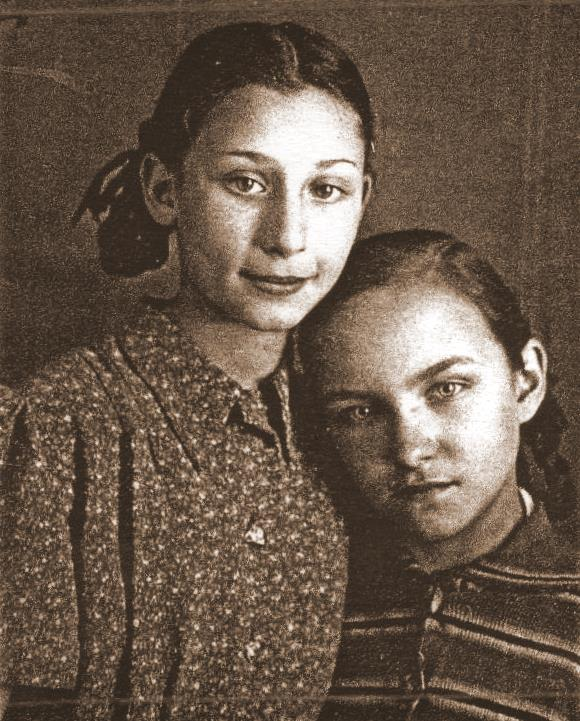
\includegraphics[width=23mm]{inc/94/2}}{    \caption{Элла Певзнер с \\Инной Платоновой. }}
    \end{minipage}
\end{figure}

\indent

\begin{figure}[h!]
    \begin{minipage}[t]{70mm}
    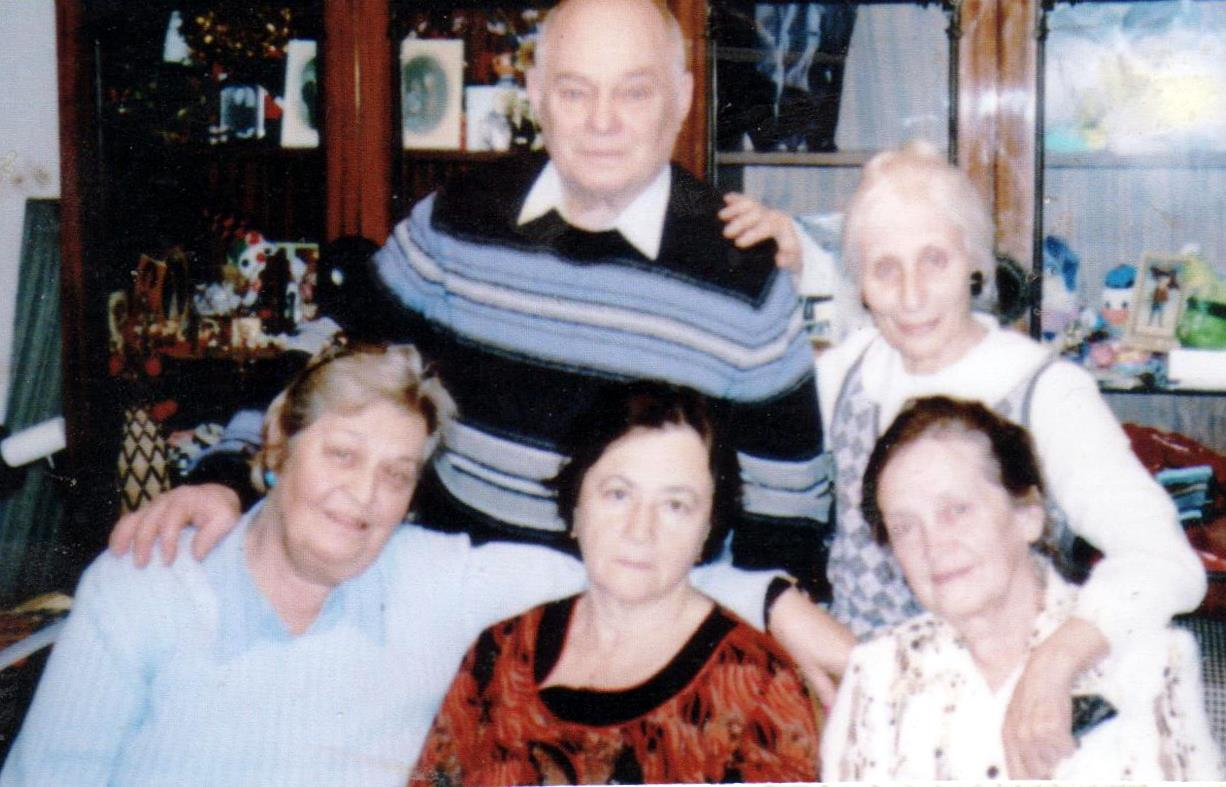
\includegraphics[width=70mm]{inc/94/1}
    \footnotesize{\textit{Э. И.. Певзнер с М. М. Плоткиным и женами М. М. Плоткина, М. В. Миникса и \\ Б. И. Моргунова.}}
    \end{minipage}
\end{figure}


\chapter{}



\textbf{Нерасшифрованные фото.} Ниже публикуются две фотографии дворовых компаний ребят 1920--1926 и 1944--1946 (ориентировочно) годов рождения.

Надеемся, что к моменту окончания подготовки Альбома удастся узнать~-- кто на них изображен. Тогда фотографии попадут в основной текст.

\vspace{10pt}

\begin{figure}[ht!]
    \begin{minipage}{80mm}
        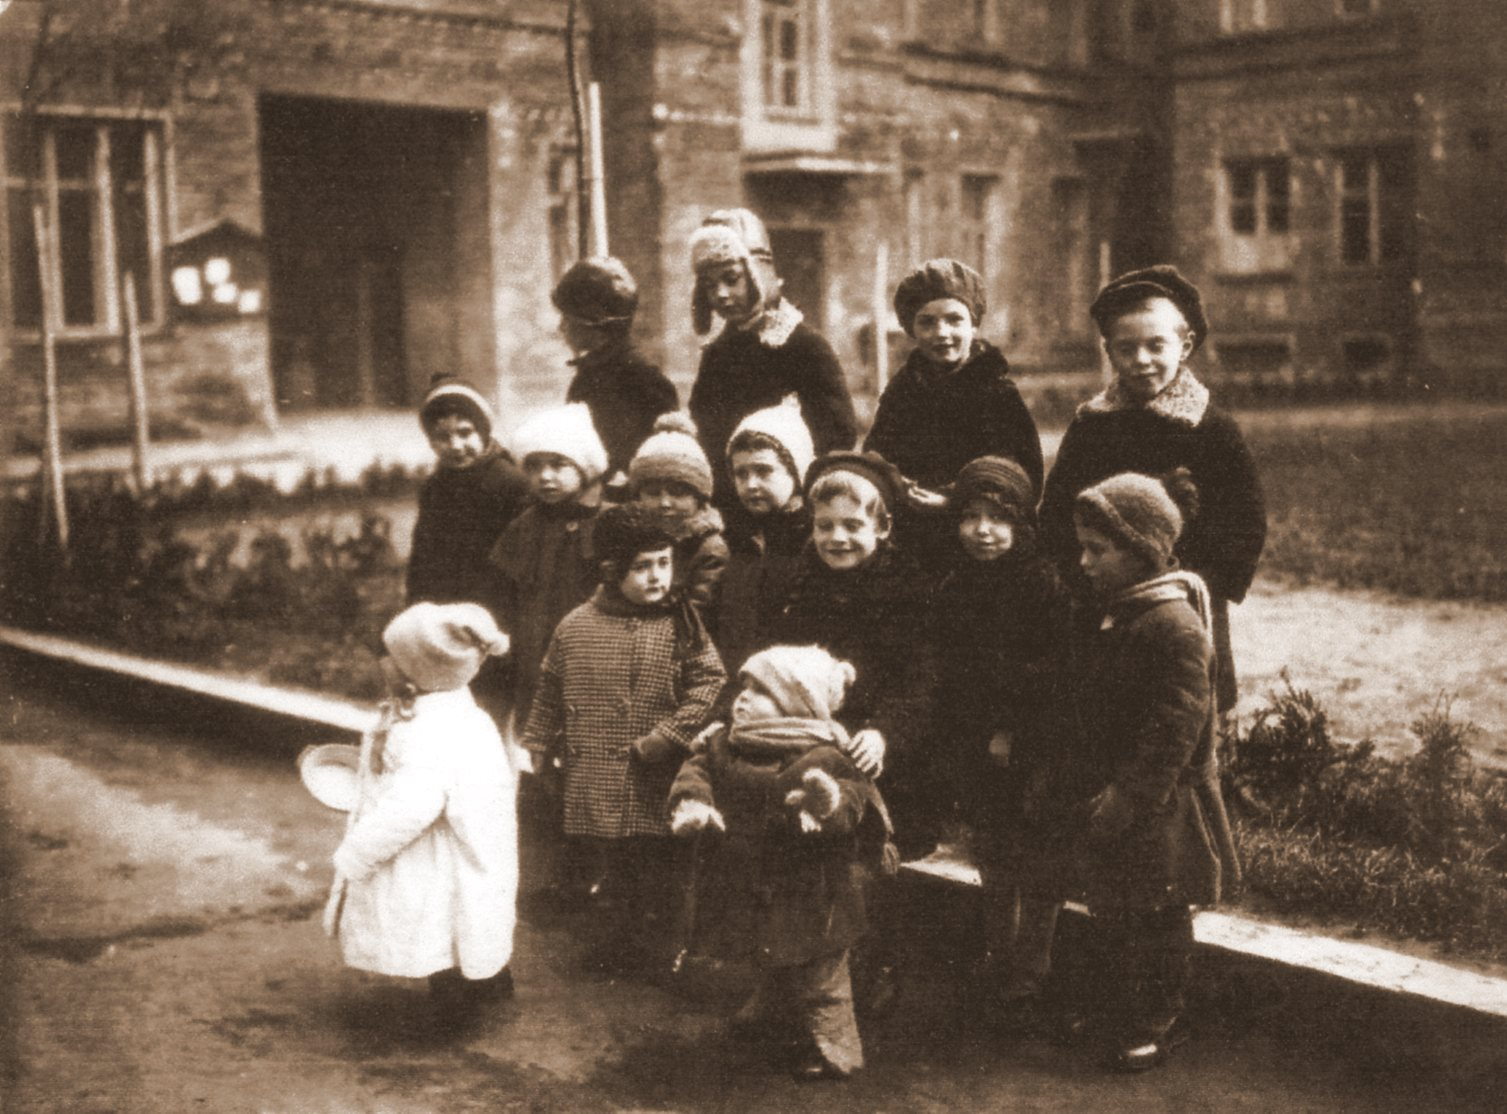
\includegraphics[width=80mm]{inc/95/1}
        \footnotesize{\textit{Наш двор. Начало тридцатых годов.}}
     \end{minipage}
\end{figure}

\vspace{10pt}

\begin{figure}[h!]
\begin{minipage}{80mm}
    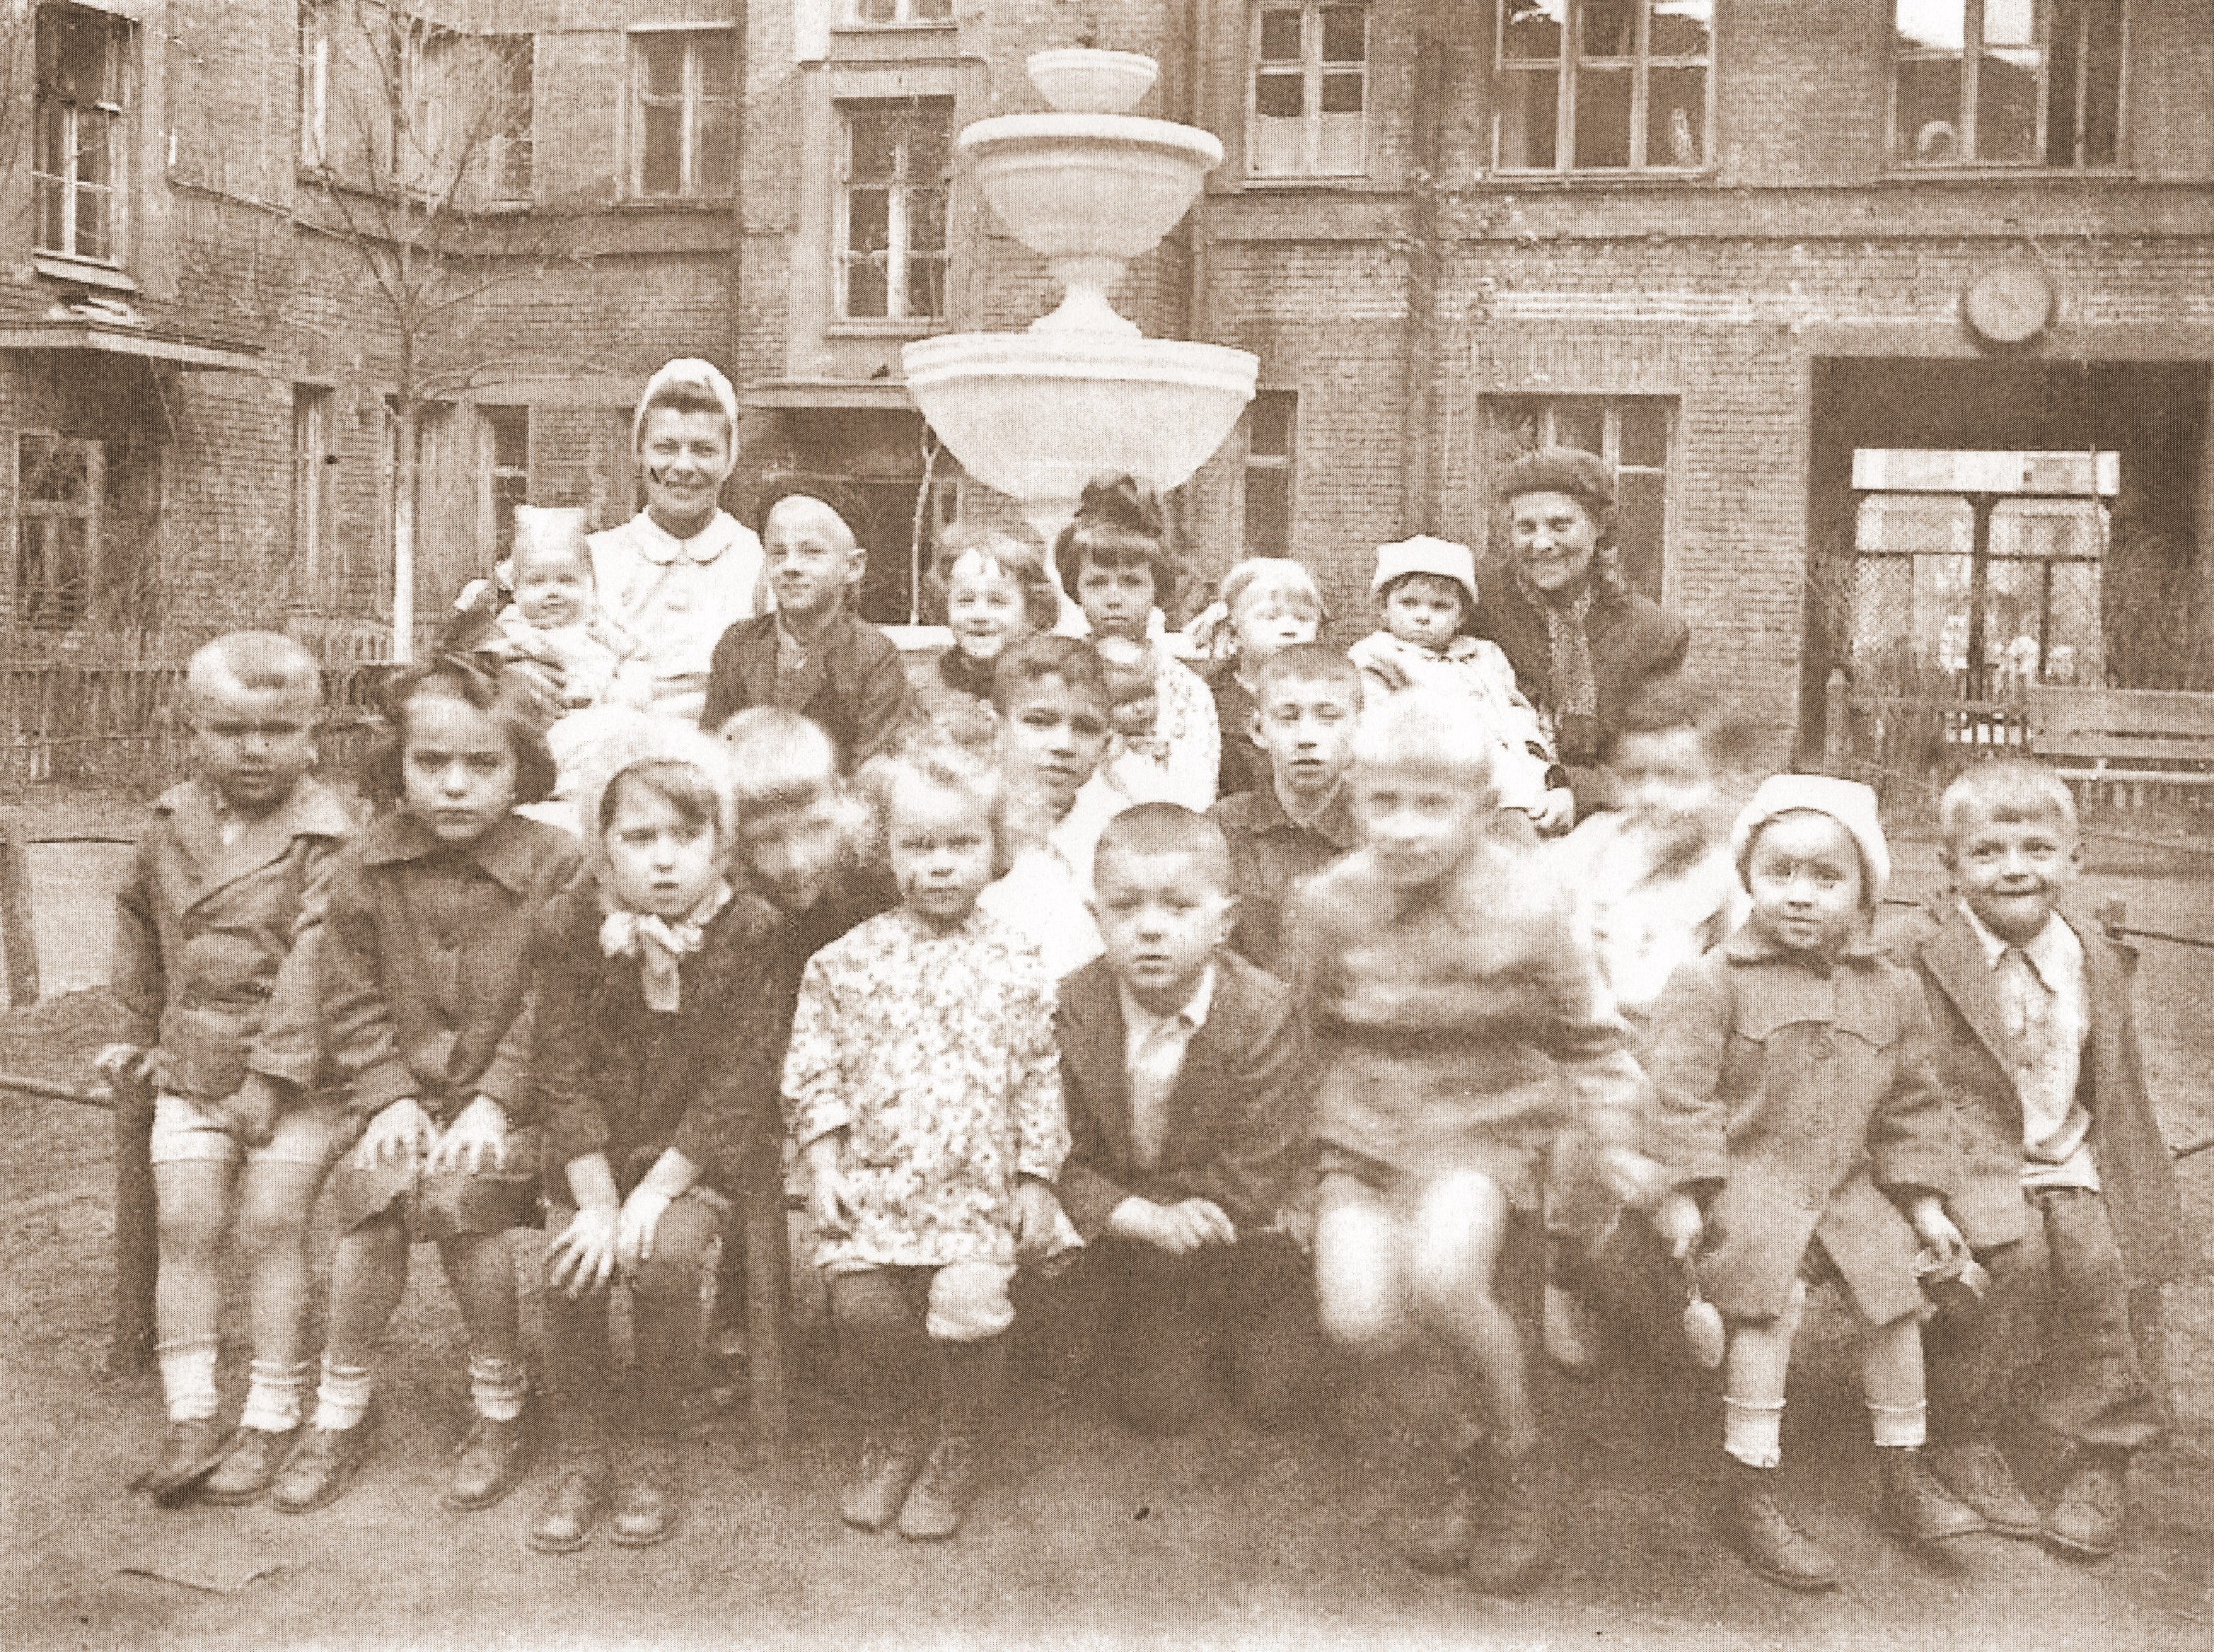
\includegraphics[width=80mm]{inc/95/2}
    \footnotesize{\textit{Наш двор. Начало пятидесятых.}}
\end{minipage}
\end{figure}



\noindent
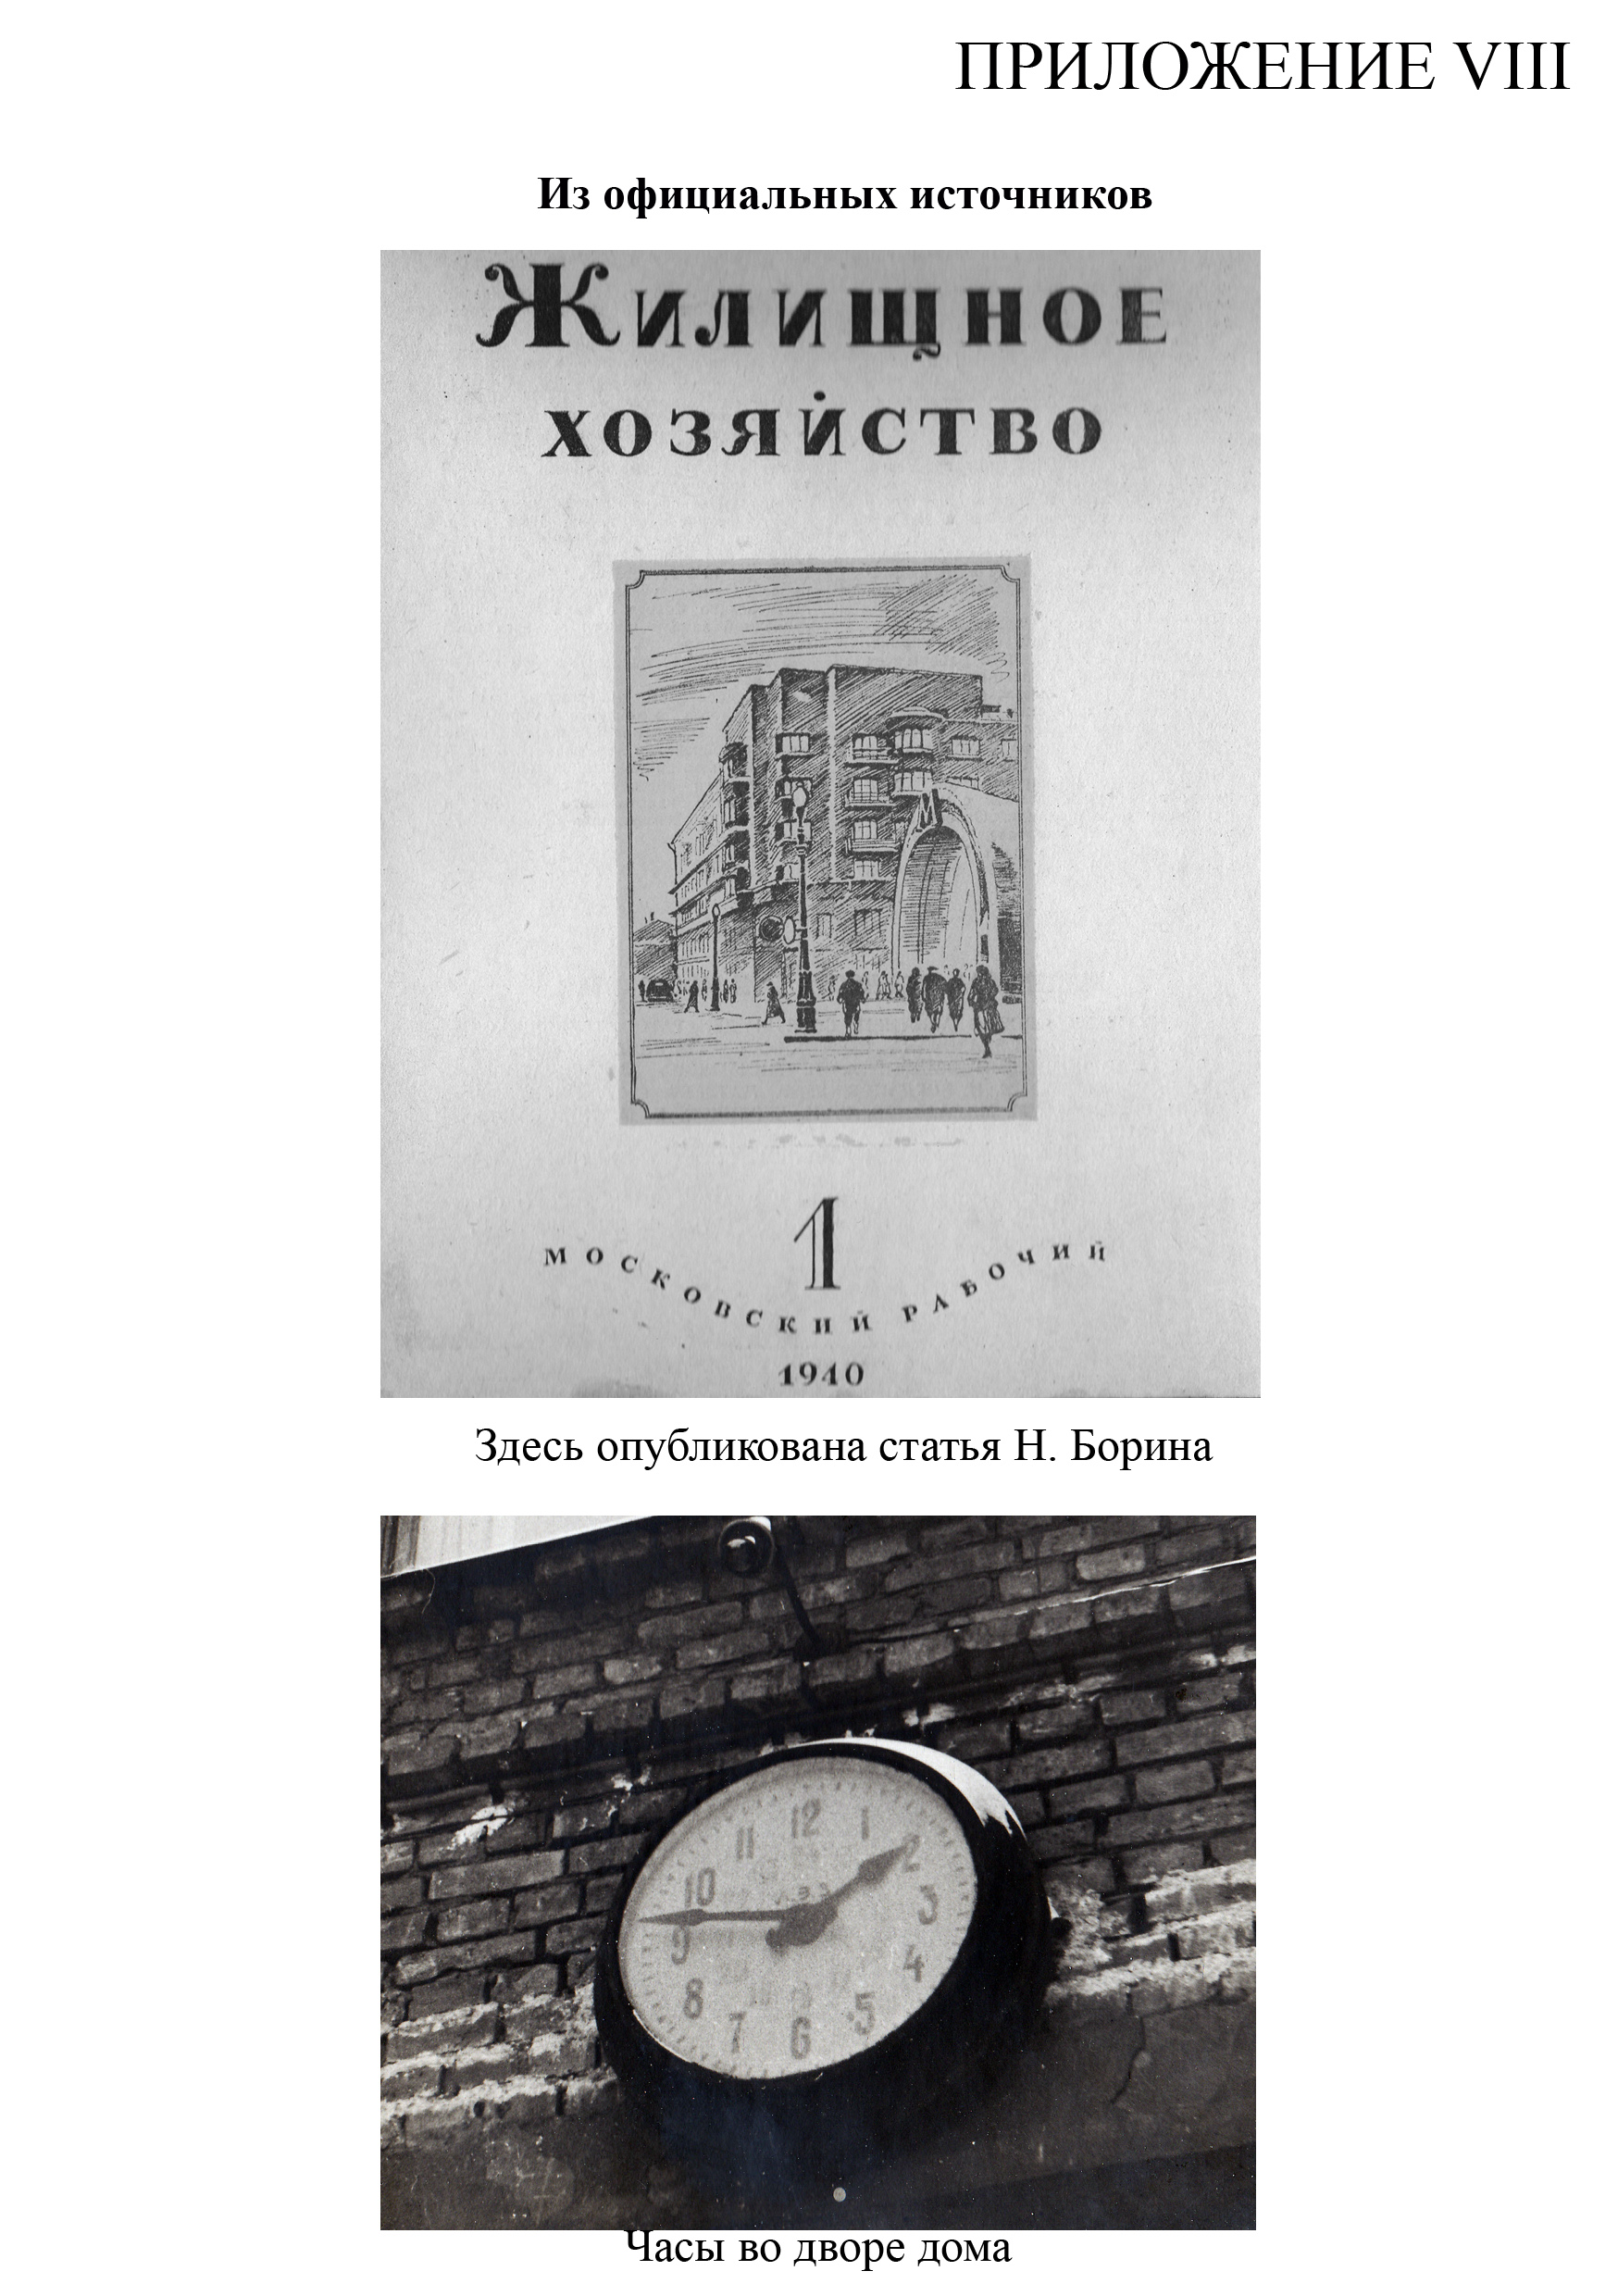
\includegraphics[width=\textwidth]{inc/p/np1.jpg}

\newpage

\noindent
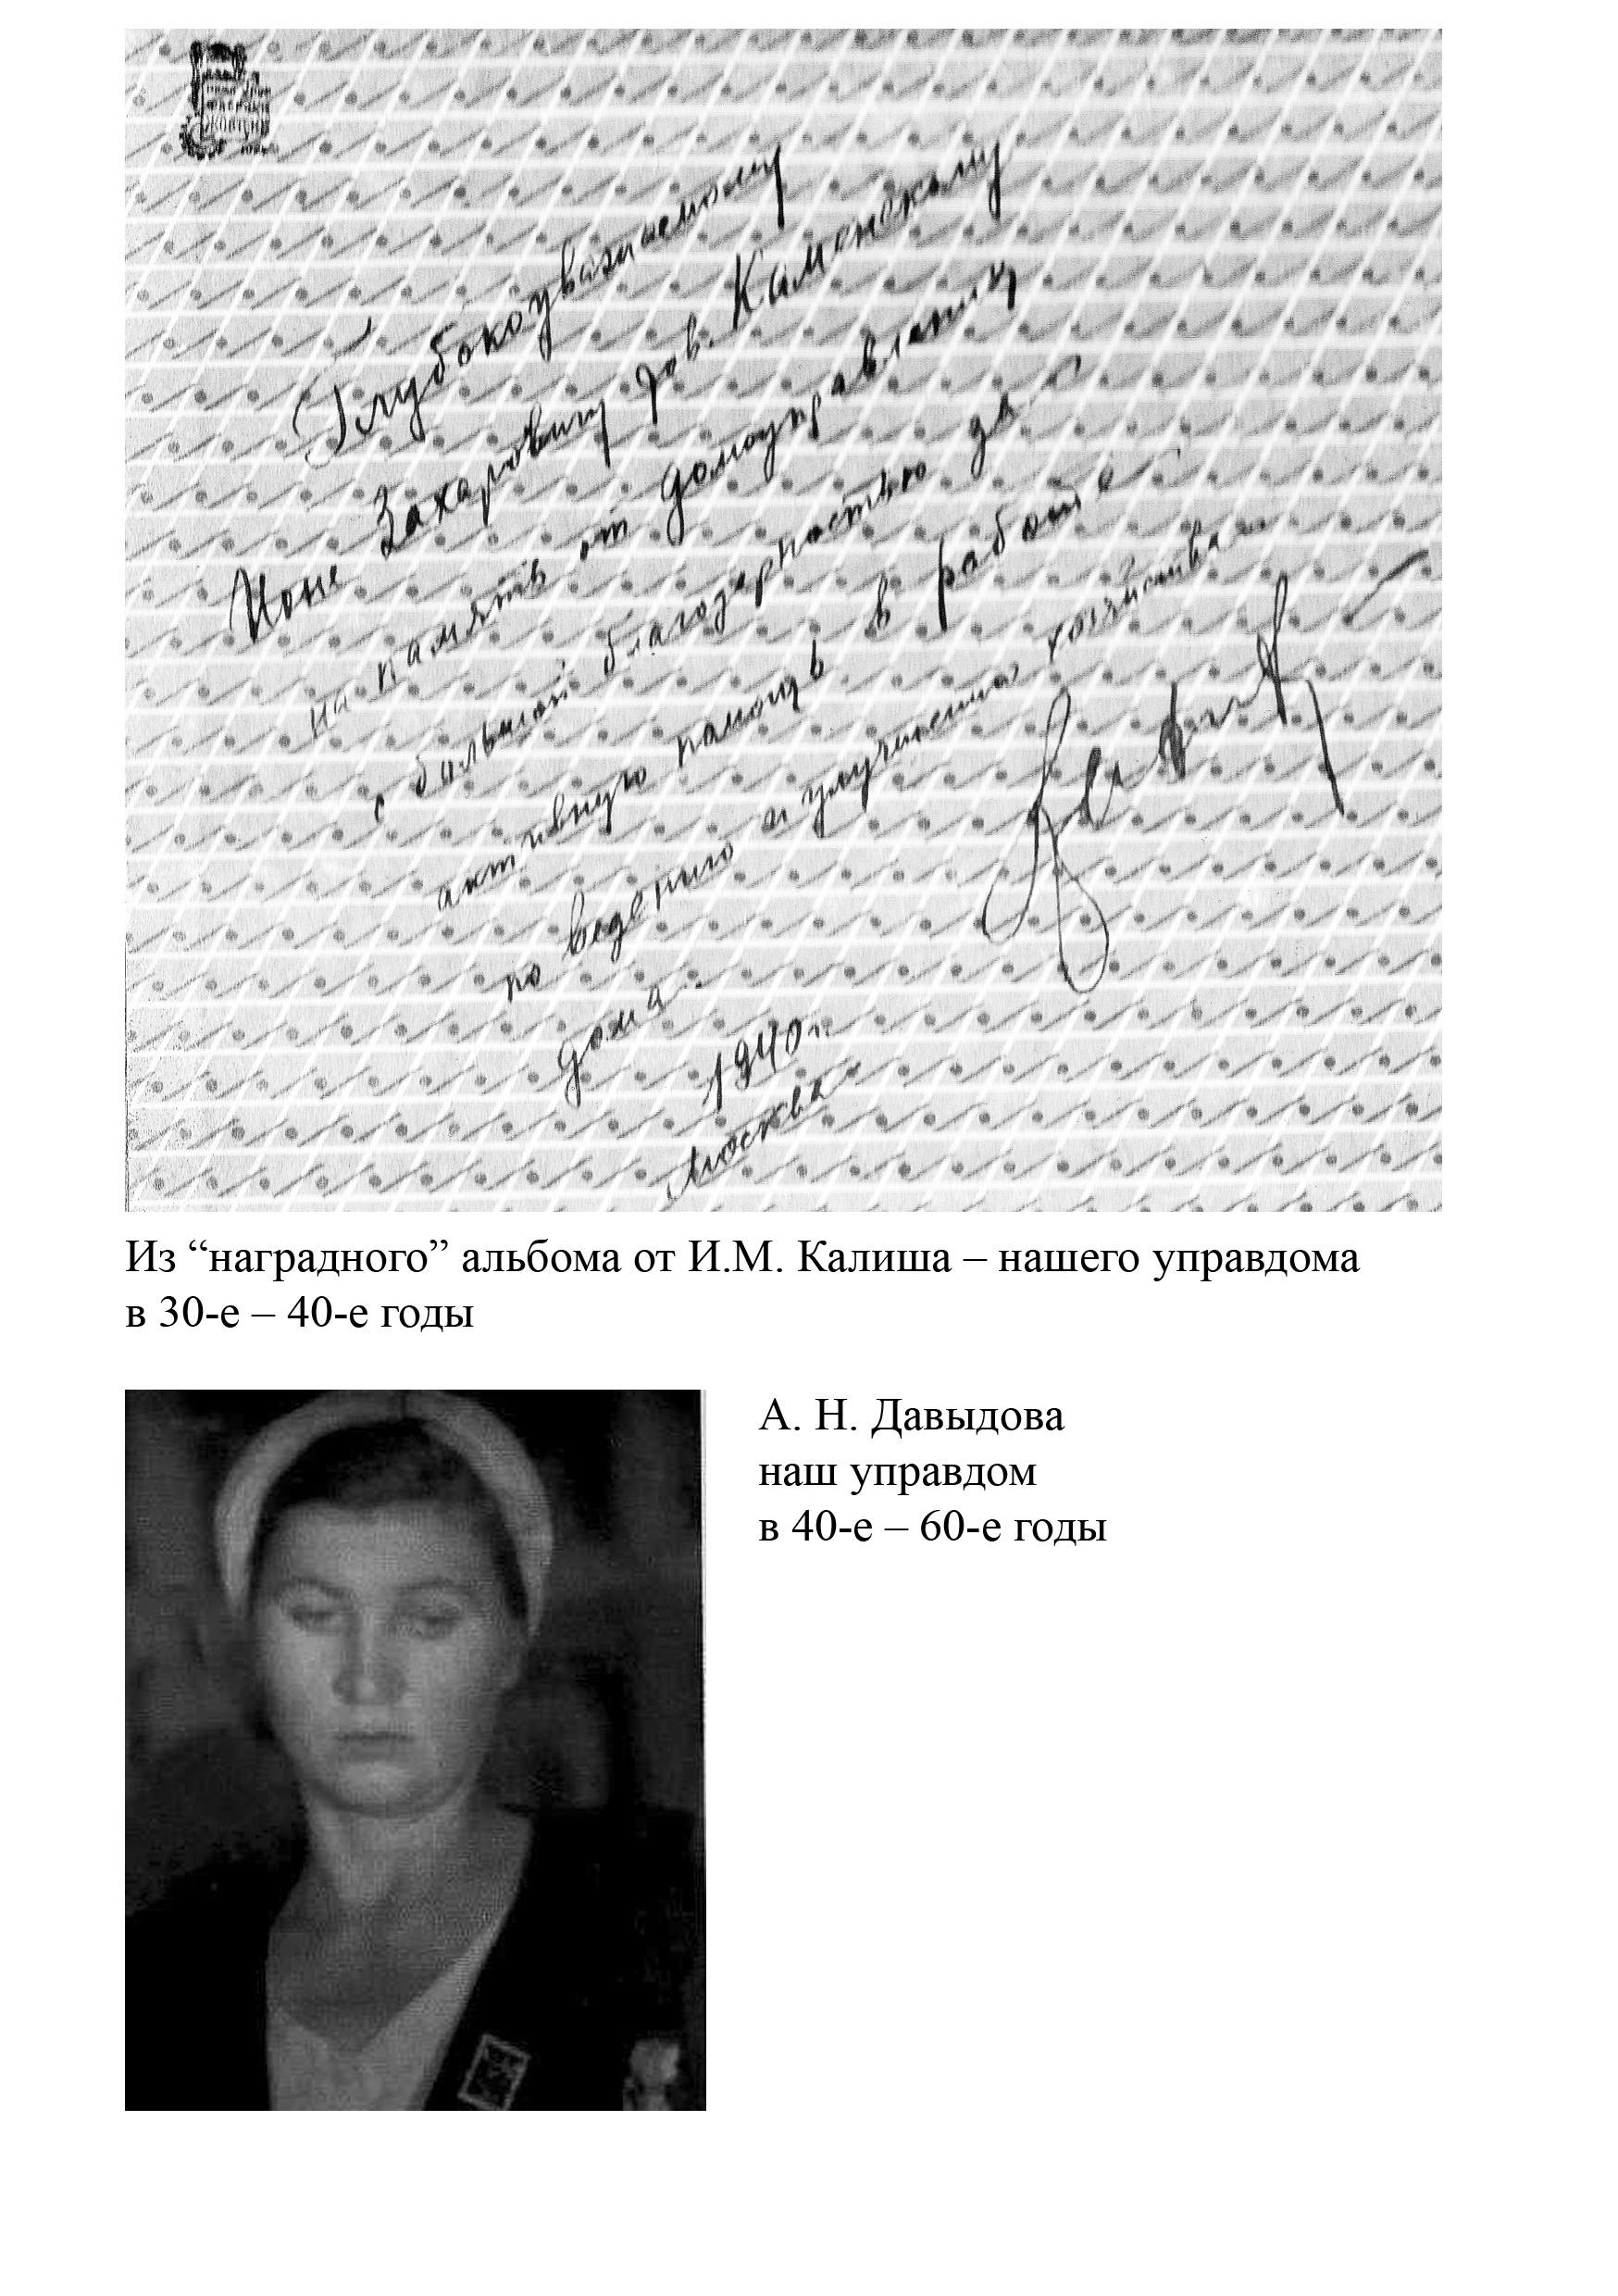
\includegraphics[width=\textwidth]{inc/p/np2.jpg}

\newpage

\noindent
\noindent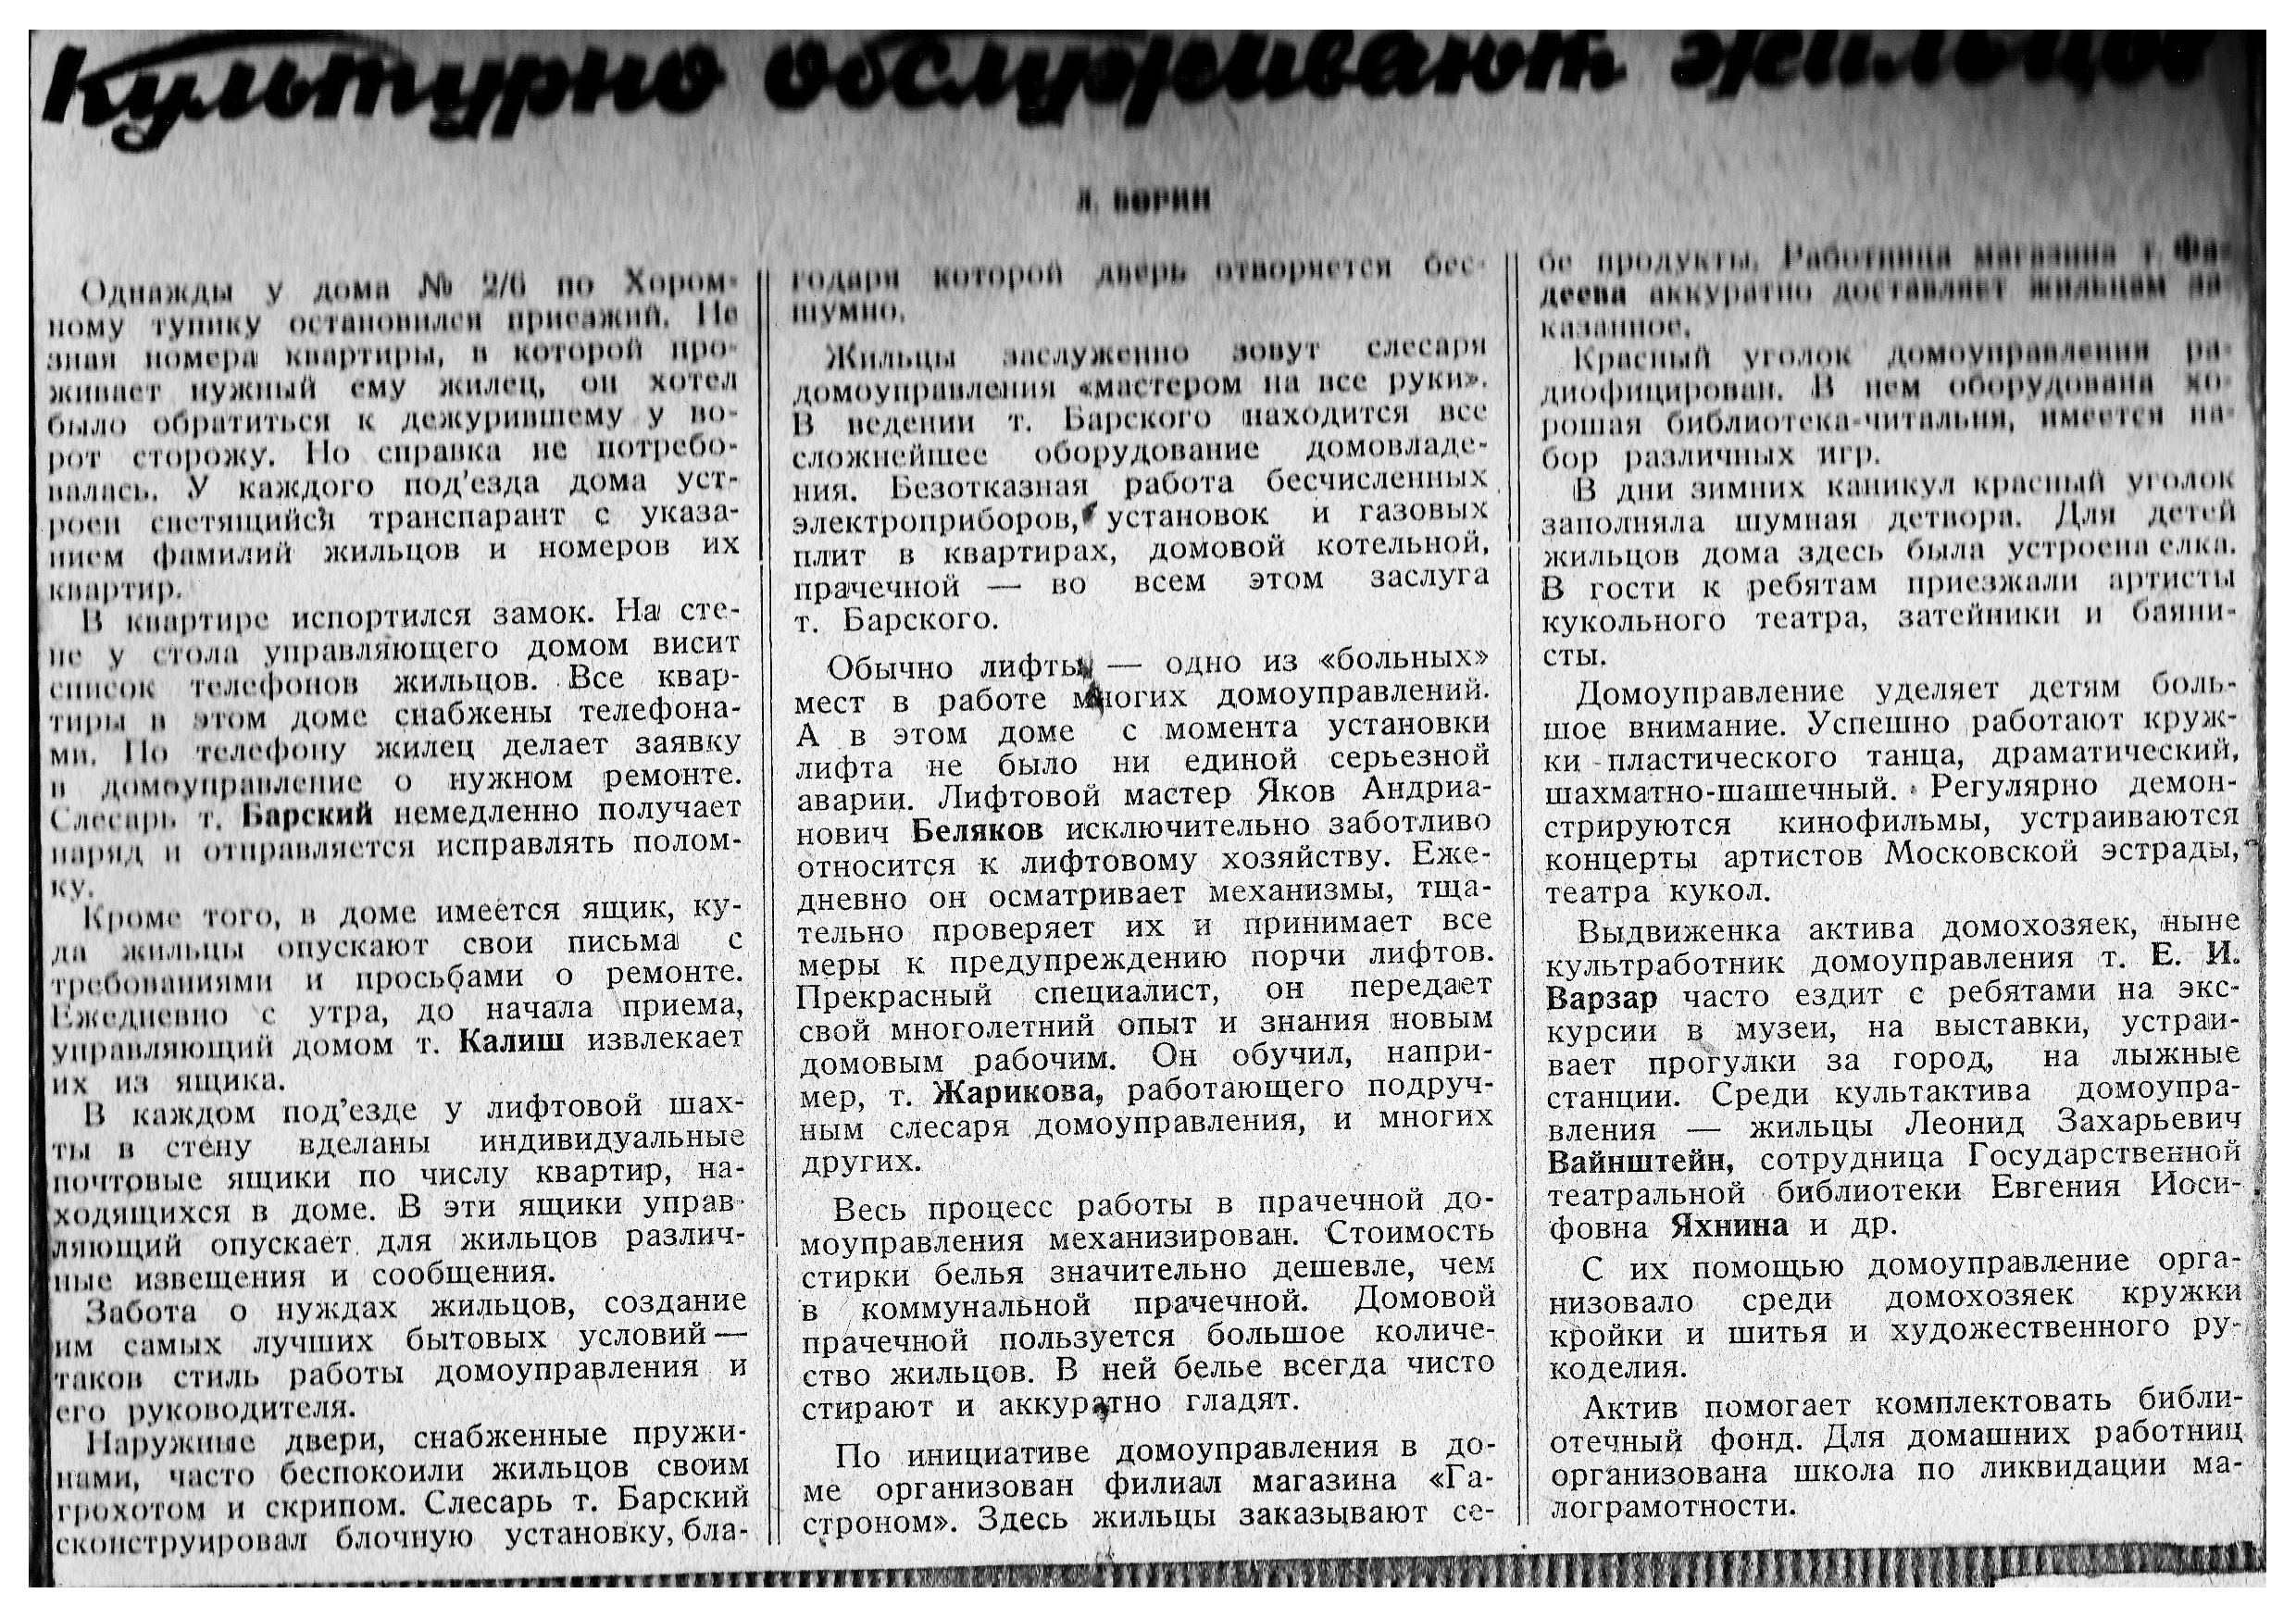
\includegraphics[width=\textheight, angle=90]{inc/p/np3.jpg}

\newpage

\noindent
\includegraphics[width=\textwidth]{inc/p/np4.jpg}

\newpage

\noindent
\includegraphics[width=\textwidth]{inc/p/np5.jpg}

\newpage

\noindent
\includegraphics[width=\textwidth]{inc/p/np6.jpg}

\newpage

\noindent
\includegraphics[width=\textwidth]{inc/p/np7.jpg}

\newpage

\noindent
\includegraphics[width=\textwidth]{inc/p/np8.jpg}

\newpage

%\setcounter{page}{105}
%\setcounter{chapter}{7}


\thispagestyle{empty} 

\begin{center}

    \textbf{\Large Содержание}

    \indent

    Предисловие \hfill 3
    
    Дворовые компании \hfill 11
    
    VIP \hfill 34
    
    Приложение I \hfill 38
    
    \hspace{20pt} Из <<Вундеркинда>> №1. 1947г. \hfill 38
    
    \hspace{20pt} Из <<Вундеркинда>> №2. 1947г. \hfill 39
    
    \hspace{20pt} Из <<Вундеркинда>> юбилейного. 1987г. \hfill 52
    
    
    {\raggedrightПриложение II. Из воспоминаний 
    
    }
    
    \hspace{93pt}О. А. Гриневского \hfill 66
    
    Приложение III. Из воспоминаний В.Б. Прейса \hfill 79

    {\raggedright Приложение IV. Из воспоминаний
    
    } 
    \hspace{93pt}М. В. Миникса \hfill 107
   
    {\raggedright Приложение V. Из воспоминаний С. Л. Кор-
    
    }
    
    \hspace{93pt}чиковой (Клейн) и др. \hfill 111
    
    Приложение VI. Из воспоминаний Э. И. Певзнер \hfill 114
    
    Приложение VII. Нерасшифрованные фото \hfill 123    
    
    Приложение VIII. Из официальных источников \hfill 124
    
    
    
\end{center}

\end{document}

%%% Local Variables:
%%% mode: latex
%%% TeX-master: t
%%% End:
